%% 
%% Copyright 2019-2021 Elsevier Ltd
%% 
%% This file is part of the 'CAS Bundle'.
%% --------------------------------------
%% 
%% It may be distributed under the conditions of the LaTeX Project Public
%% License, either version 1.2 of this license or (at your option) any
%% later version.  The latest version of this license is in
%%    http://www.latex-project.org/lppl.txt
%% and version 1.2 or later is part of all distributions of LaTeX
%% version 1999/12/01 or later.
%% 
%% The list of all files belonging to the 'CAS Bundle' is
%% given in the file `manifest.txt'.
%% 
%% Template article for cas-dc documentclass for 
%% double column output.

\documentclass[fleqn]{cas-sc}

\usepackage{lipsum}
\usepackage{tikz}
\usetikzlibrary{shapes, snakes, calc}
\usepackage{longtable}

% If the frontmatter runs over more than one page
% use the longmktitle option.

%\documentclass[a4paper,fleqn,longmktitle]{cas-dc}

%\usepackage[numbers]{natbib}
%\usepackage[authoryear]{natbib}
\usepackage[authoryear,longnamesfirst]{natbib}

%%%Author macros
\def\tsc#1{\csdef{#1}{\textsc{\lowercase{#1}}\xspace}}
\tsc{WGM}
\tsc{QE}
%%%

% Uncomment and use as if needed
%\newtheorem{theorem}{Theorem}
%\newtheorem{lemma}[theorem]{Lemma}
%\newdefinition{rmk}{Remark}
%\newproof{pf}{Proof}
%\newproof{pot}{Proof of Theorem \ref{thm}}

\begin{document}
\let\WriteBookmarks\relax
\def\floatpagepagefraction{1}
\def\textpagefraction{.001}

% Short title
\shorttitle{Ambulance Dispatch}    

% Short author
%\shortauthors{Burkman, Jin, Abuhijleh, and Sun}  
\shortauthors{First, Second, Third, Fourth}  

% Main title of the paper
\title [mode = title]{Modeling the Need for an Ambulance based on Automated Crash Reports from Cell Phones}  

% Title footnote mark
% eg: \tnotemark[1]
%\tnotemark[<tnote number>] 
%\tnotemark[1] 

% Title footnote 1.
% eg: \tnotetext[1]{Title footnote text}
%\tnotetext[1]{Working Title} 

% First author
%
% Options: Use if required
% eg: \author[1,3]{Author Name}[type=editor,
%       style=chinese,
%       auid=000,
%       bioid=1,
%       prefix=Sir,
%       orcid=0000-0000-0000-0000,
%       facebook=<facebook id>,
%       twitter=<twitter id>,
%       linkedin=<linkedin id>,
%       gplus=<gplus id>]

%\author[<aff no>]{<author name>}[<options>]
%\author[1,2]{J. Bradford Burkman}[]
\author[1,2]{First Author}[]
% Footnote of the first author
%\fnmark[1]
% Corresponding author indication
%\cormark[1]
% Email id of the first author
%\ead{bradburkman@gmail.com}
\ead{FirstAuthor@gmail.com}
% URL of the first author
%\ead[url]{http://www.github.com/bburkman}

% Credit authorship
% eg: \credit{Conceptualization of this study, Methodology, Software}
% Options: conceptualization; data curation; formal analysis; funding acquisition; investigation; methodology; project administration; resources; software; supervision; validation; visualization; writing – original draft; and writing – review and editing.
\credit{Conceptualization, Investigation, Writing - original draft, Visualization}


%\author[1]{Miao Jin}[]
\author[1]{Second Author}[]
\credit{Supervision, Methodology, Writing - review and editing}

%\author[1,3]{Malek Abuhijleh}[]
\author[1,3]{Third Author}[]
\credit{Investigation, Methodology}

%\author[3]{Xiaoduan Sun}[]
\author[3]{Fourth Author}[]
\credit{Data curation, Writing - review and editing}






%\affiliation[1]{organization={School of Computing and Informatics, University of Louisiana at Lafayette},
\affiliation[1]{organization={School, University},
%            addressline={301 E. Lewis St}, 
%            city={Lafayette},
%          citysep={}, % Uncomment if no comma needed between city and postcode
%            state={LA},
%            postcode={70503}, 
%            country={USA}
            }

% Address/affiliation
%\affiliation[2]{organization={Louisiana School for Math, Science, and the Arts},
\affiliation[2]{organization={Other School},
%            addressline={715 University Pkwy}, 
%            city={Natchitoches},
%          citysep={}, % Uncomment if no comma needed between city and postcode
%            state={LA},
%            postcode={71457}, 
%            country={USA}
            }

%\affiliation[3]{organization={Department of Civil Engineering, University of Louisiana at Lafayette},
\affiliation[3]{organization={Other Department, University},
%            addressline={131 Rex St}, 
%            city={Lafayette},
%          citysep={}, % Uncomment if no comma needed between city and postcode
%            state={LA},
%            postcode={70504}, 
%            country={USA}
            }




% For a title note without a number/mark
%\nonumnote{}

% Here goes the abstract
\begin{abstract}
%%%%% Abstract
% I found an abstract in TRpC June 2022 with 365 words.
%Put abstract here.
%%%%% Abstract
% I found an abstract in TRpC June 2022 with 365 words.
New Google Pixel phones can automatically notify an emergency dispatcher if the phone detects the deceleration profile of a vehicular crash.  Most crash notifications come from an eyewitness who can say whether an ambulance is needed, but the automated notification from the cell phone cannot provide that information directly.  Should the dispatcher immediately send an ambulance before receiving an eyewitness report?  There are three options: Always, Wait, and Sometimes.  The ``Always'' option refers to sending an ambulance to every automatically reported crash, even though most of them will not be needed.  In the ``Wait'' option, the dispatcher sends police, but always waits for a call from an eyewitness (perhaps the police) before sending an ambulance.  In the ``Sometimes'' option, the dispatcher relies on a machine learning recommendation system to decide whether to immediately dispatch an ambulance, reserving the option to send one later based on an eyewitness report.

%This paper explores one option for building a machine learning (ML) model for making a recommendation in the ``Sometimes'' option.  The model gives the probability (based on the available information) that a crash requires an ambulance.  If the probability that an ambulance is needed is above some chosen threshold, the method will recommend dispatching an ambulance immediately; below that threshold, the dispatcher should wait to hear from an eyewitness. 


This paper explores one option for building a machine learning (ML) model for making a recommendation in the ``Sometimes'' option.    Our goal is to build a model that returns, for each feature vector (crash report, sample), a value $p \in [0,1]$ that increases with the probability that the person needs an ambulance.  Then we choose a threshold $\theta$ such that we immediately send ambulances to those automated crash reports with $p > \theta$, and wait for eyewitness confirmation for those reports with $p < \theta$. In an actual implementation, the choice of $\theta$ is political, not technical, so we consider and interpret several options.  

Once a threshold has been chosen, the costs of the false positives (FP) and false negatives (FN) in dispatching ambulances are very different.  The cost of sending an ambulance when one is not needed (FP) is measured in dollars, but the cost of not promptly sending an ambulance when one is needed (FN) is measured in lives.  Choosing such a tradeoff threshold is ethically problematic, but governments implicitly choose such a tradeoff when they set budgets for emergency services.  

We consider and interpret several options for the decision threshold $\theta$ based on the political consideration, ``How much will it cost?''  How many automated ambulance dispatches are we willing to fund (FP + TP) for each one of them that's actually needed (TP)?  We will explore two versions of that question, the total and the marginal.  


%some of which consider a relationship between the total number of FP and FN up to that value of $p$, and others consider the marginal relationship around that value of $p$.  Once the threshold criteria are chosen, the problem turns to choosing and tuning a model that best satisfies the tradeoff, saving both money and lives.  

%We consider the factors in determining the threshold.  The costs of the false positives (FP) and false negatives (FN) in dispatching ambulances are very different.  The cost of sending an ambulance when one is not needed (FP) is measured in dollars, but the cost of not promptly sending an ambulance when one is needed (FN) is measured in lives.  Choosing such a tradeoff threshold is ethically problematic, but governments implicitly make such a tradeoff when they set budgets for emergency and medical services.  To demonstrate the method in this paper, we have arbitrarily chosen a cutoff of 33\%, that there is a 1 in 3 chance that a dispatched ambulance would be needed (TP) and a 2 in 3 chance that it would not (FP).  We formulate our marginal ethical tradeoff rate as   $\omega = \Delta FP/\Delta TP = 2.0$.  We incorporated $\omega$ into the model in the class weight and in the decision threshold.  

We show that the quality of the model depends highly on the input data available, and we considered three levels of data availability.  The ``Easy'' level includes time of day and weather, data the emergency dispatcher has before the notification.  The ``Medium'' level adds the age and sex of the cell phone user and information about the location.  The ``Hard'' level adds information about the vehicle likely to be driven by the cell phone user and detailed and temporal information about the location, like lighting conditions and whether it is currently a work zone.  

We used the data of the Crash Report Sampling System (CRSS) to validate our approach.  We have applied new methods (for this dataset in the literature) to handle missing data, and we have investigated several methods for handling the data imbalance.  To promote discussion and future research, we have included all of the code we used in our analysis.  
%\vskip 1in

\end{abstract}

% Use if graphical abstract is present
%\begin{graphicalabstract}
%\includegraphics{}
%\end{graphicalabstract}

% Research highlights
\begin{highlights}
	\item  Supports transferability and benchmarking of different approaches on a public large-scale dataset.  We have attached the code we used to perform the analysis on data from the Crash Report Sampling System (CRSS).  
	\item Novel Application motivated by Emerging Technology:  Machine Learning Classification Models for Dispatching Ambulances based on Automated Crash Reports
	\item New Use of Dataset:  Used Crash Report Sampling System (CRSS), which has imputed missing values for some features, but not all of the ones we wanted to use.  For the first time we have seen, we used the software the CRSS authors use for multiple imputation (IVEware) to impute missing values in more features, then compared the results with other methods of imputation.
	\item Explicit Incorporation of Imbalanced Costs
	\item Explicit Incorporation of Political Dimensions
	\item Perennial Machine Learning Challenge:  Imbalanced Datasets
\end{highlights}

% Keywords
% Each keyword is seperated by \sep
\begin{keywords}
 \sep Automated crash notification 
 \sep Ambulance dispatch 
 \sep Emergency medical services  
 \sep Machine learning 
 \sep Imbalanced Cost 
 \sep Imbalanced Data 
 \sep Imputation
\end{keywords}

\maketitle

% Main text

%%%%%
%
% To Do
%
%
%%%%%

%%%%% Henry's Questions 23 May 2023
%\section{Henry's Questions 23 May 2023}
%\subsection{Abstract}

I made most of the changes you suggested for the abstract.  (Above)

I changed ``police'' to ``emergency dispatcher'' rather than ``911 dispatcher'' so as to not annoy the people (like the editor) in countries that use 119.  

I think the abstract is now too long, but that's a problem for later.  

\subsection{Threshold, Prior and Posterior Probabilities}

Thank you for your summary of the decision problem.  I will adapt the language here. I will try to answer your questions through an example.   Please let me know if I don't understand it well.  

\

I'm trying to understand the $\hat{p}$ you used.  I understand $p$ as the probability that a given sample is in Class 1.  Because you related $\hat{p}$ to $\pi_1$, I suspect what $\hat{p}$ means is the percentage of samples the model (with our choice of decision threshold) classifies as being in Class 1.  Is that correct?  In the big chart below, 

$$\hat{p} = \frac{FP + TP}{TN + FP + FN + TP}$$

\

Using the CRSS dataset, our problem has two outcomes.  

\begin{center}
\begin{tabular}{llll}
	Class 0 & ``No ambulance needed'' & $\pi_0 \approx 85\%$ \cr
	Class 1 & ``Ambulance needed'' & $\pi_1 \approx 15\%$ \cr
\end{tabular}
\end{center}

We will run several models, but a particular model gives, for each input vector (sample), a probability $p$ that the sample is in Class 1.  We want to pick a discrimination threshold (decision threshold) $\theta$ such that if for a particular crash notification $p > \theta$, then our recommendation system recommends that the emergency dispatcher send an ambulance.  

Below is the test results of one of our best models, the Balanced Random Forest Classifier with no class weights ($\alpha = 0.5$).  The histogram gives, for each range of $p$, the percent of the total dataset with Class 0 (Neg) and Class 1 in that range of $p$.  

Until we choose the discrimination threshold $\theta$, we can't have a confusion matrix.  Once we choose $\theta$, then all of the negative samples with $p< \theta$ are true negatives, and all of the negative samples with $p > \theta$ are false positives; conversely for the positive samples.  

\


\noindent\begin{tabular}{@{\hspace{-6pt}}p{4.5in} @{\hspace{-6pt}}p{2.0in}}
	\vskip 0pt
	\qquad \qquad Raw Model Output
	
	\input{../Keras/Images/BRFC_Hard_Tomek_0_alpha_0_5_v1_Test_Pred_Wide.pgf}
&
	\vskip 0pt
	\qquad \qquad ROC Curve
	
	\input{../Keras/Images/BRFC_Hard_Tomek_0_alpha_0_5_v1_Test_ROC.pgf}
\end{tabular}

\
	
In the table below,

\begin{itemize}
	\item The first three columns are the same information as in the histogram.  ``Neg'' (``Pos'') is the number of negative (positive) samples whose probability of being in Class 1 is in that range of $p$.  
	\item The fourth column, ``Neg/Pos,'' is the number of unneeded ambulances sent for each needed ambulance sent, for samples with $p$ in that range.    This is the marginal cost of having $\theta$ below this value of $p$.  These values are given in this plot, emphasizing where Neg/Pos = $\Delta FP/\Delta TP = 2$. 
	
\input{../Keras/Images/BRFC_Hard_Tomek_0_alpha_0_5_v1_Test_FP_TP.pgf}	

The ``TN,'' ``FP,'' ``FN,'' and ``TP'' columns are the confusion matrix if we choose $\theta$ in that range of $p$.  

	\item The seventh column, ``FP/TP'' is related, but it's the total cost in terms of how many unneeded ambulances we'd send for each one we needed if $\theta$ were that value of $p$.  
	
	\item The last three columns are Precision, Recall, and $\hat{p}$ (If I understand $\hat{p}$ correctly).
\end{itemize}



\begin{center}
\begin{tabular}{rrrrrrrrrrrrrr}
\toprule
{} &     Neg &    Pos & mPrec &       TN &       FP &      FN &      TP &  Prec &   Rec & $\hat{p}$ \\
p    &         &        &       &          &          &         &         &       &       &           \\
\midrule
0.00 &     107 &      0 &  0.00 &      107 &  180,138 &       0 &  33,825 &  0.16 &  1.00 &      1.00 \\
0.05 &   2,287 &     20 &  0.01 &    2,394 &  177,851 &      20 &  33,805 &  0.16 &  1.00 &      0.99 \\
0.10 &   6,177 &     62 &  0.01 &    8,571 &  171,674 &      82 &  33,743 &  0.16 &  1.00 &      0.96 \\
0.15 &  10,435 &    188 &  0.02 &   19,006 &  161,239 &     270 &  33,555 &  0.17 &  0.99 &      0.91 \\
0.20 &  13,424 &    388 &  0.03 &   32,430 &  147,815 &     658 &  33,167 &  0.18 &  0.98 &      0.85 \\
0.25 &  15,746 &    619 &  0.04 &   48,176 &  132,069 &   1,277 &  32,548 &  0.20 &  0.96 &      0.77 \\
0.30 &  17,256 &    923 &  0.05 &   65,432 &  114,813 &   2,200 &  31,625 &  0.22 &  0.93 &      0.68 \\
0.35 &  17,841 &  1,320 &  0.07 &   83,273 &   96,972 &   3,520 &  30,305 &  0.24 &  0.90 &      0.59 \\
0.40 &  17,355 &  1,690 &  0.09 &  100,628 &   79,617 &   5,210 &  28,615 &  0.26 &  0.85 &      0.51 \\
0.45 &  16,597 &  2,042 &  0.11 &  117,225 &   63,020 &   7,252 &  26,573 &  0.30 &  0.79 &      0.42 \\
0.50 &  14,984 &  2,470 &  0.14 &  132,209 &   48,036 &   9,722 &  24,103 &  0.33 &  0.71 &      0.34 \\
0.55 &  12,810 &  2,725 &  0.18 &  145,019 &   35,226 &  12,447 &  21,378 &  0.38 &  0.63 &      0.26 \\
0.60 &  10,493 &  2,972 &  0.22 &  155,512 &   24,733 &  15,419 &  18,406 &  0.43 &  0.54 &      0.20 \\
0.65 &   8,062 &  3,037 &  0.27 &  163,574 &   16,671 &  18,456 &  15,369 &  0.48 &  0.45 &      0.15 \\
0.70 &   6,040 &  2,953 &  0.33 &  169,614 &   10,631 &  21,409 &  12,416 &  0.54 &  0.37 &      0.11 \\
0.75 &   4,144 &  2,893 &  0.41 &  173,758 &    6,487 &  24,302 &   9,523 &  0.59 &  0.28 &      0.07 \\
0.80 &   2,902 &  2,627 &  0.48 &  176,660 &    3,585 &  26,929 &   6,896 &  0.66 &  0.20 &      0.05 \\
0.85 &   1,801 &  2,530 &  0.58 &  178,461 &    1,784 &  29,459 &   4,366 &  0.71 &  0.13 &      0.03 \\
0.90 &   1,043 &  2,166 &  0.67 &  179,504 &      741 &  31,625 &   2,200 &  0.75 &  0.07 &      0.01 \\
0.95 &     587 &  1,597 &  0.73 &  180,091 &      154 &  33,222 &     603 &  0.80 &  0.02 &      0.00 \\
1.00 &     154 &    603 &  0.80 &  180,245 &        0 &  33,825 &       0 &   nan &  0.00 &      0.00 \\
\bottomrule
\end{tabular}
}
\end{center}

Here I've zoomed in on three smaller ranges.  Interestingly, it's not useful to zoom in further, because most values of $p$ given by this implementation of the classifier are only given to two digits.  

\begin{center}
\begin{tabular}{rrrrrrrrrrrrrr}
\toprule
{} &    Neg &  Pos & Neg/Pos &       TN &       FP &      FN &      TP & FP/TP & Prec. &  Rec. & $\hat{p}$ \\
p    &        &      &         &          &          &         &         &       &       &       &           \\
\midrule
0.48 &  2,990 &  453 &    6.60 &  126,315 &   53,930 &   8,688 &  25,137 &  2.15 &  0.32 &  0.74 &      0.37 \\
0.49 &  3,020 &  533 &    5.67 &  129,335 &   50,910 &   9,221 &  24,604 &  2.07 &  0.33 &  0.73 &      0.35 \\
0.50 &  2,874 &  501 &    5.74 &  132,209 &   48,036 &   9,722 &  24,103 &  1.99 &  0.33 &  0.71 &      0.34 \\
0.51 &  2,804 &  533 &    5.26 &  135,013 &   45,232 &  10,255 &  23,570 &  1.92 &  0.34 &  0.70 &      0.32 \\
\hline
0.64 &  1,582 &  586 &    2.70 &  162,135 &   18,110 &  17,838 &  15,987 &  1.13 &  0.47 &  0.47 &      0.16 \\
0.65 &  1,439 &  618 &    2.33 &  163,574 &   16,671 &  18,456 &  15,369 &  1.08 &  0.48 &  0.45 &      0.15 \\
0.66 &  1,376 &  561 &    2.45 &  164,950 &   15,295 &  19,017 &  14,808 &  1.03 &  0.49 &  0.44 &      0.14 \\
0.67 &  1,288 &  637 &    2.02 &  166,238 &   14,007 &  19,654 &  14,171 &  0.99 &  0.50 &  0.42 &      0.13 \\
0.68 &  1,241 &  554 &    2.24 &  167,479 &   12,766 &  20,208 &  13,617 &  0.94 &  0.52 &  0.40 &      0.12 \\
0.69 &  1,082 &  631 &    1.71 &  168,561 &   11,684 &  20,839 &  12,986 &  0.90 &  0.53 &  0.38 &      0.12 \\
0.70 &  1,053 &  570 &    1.85 &  169,614 &   10,631 &  21,409 &  12,416 &  0.86 &  0.54 &  0.37 &      0.11 \\
0.71 &    922 &  587 &    1.57 &  170,536 &    9,709 &  21,996 &  11,829 &  0.82 &  0.55 &  0.35 &      0.10 \\
\hline
0.76 &    664 &  558 &    1.19 &  174,422 &    5,823 &  24,860 &   8,965 &  0.65 &  0.61 &  0.27 &      0.07 \\
0.77 &    627 &  524 &    1.20 &  175,049 &    5,196 &  25,384 &   8,441 &  0.62 &  0.62 &  0.25 &      0.06 \\
0.78 &    585 &  532 &    1.10 &  175,634 &    4,611 &  25,916 &   7,909 &  0.58 &  0.63 &  0.23 &      0.06 \\
0.79 &    568 &  529 &    1.07 &  176,202 &    4,043 &  26,445 &   7,380 &  0.55 &  0.65 &  0.22 &      0.05 \\
0.80 &    458 &  484 &    0.95 &  176,660 &    3,585 &  26,929 &   6,896 &  0.52 &  0.66 &  0.20 &      0.05 \\
0.81 &    429 &  514 &    0.83 &  177,089 &    3,156 &  27,443 &   6,382 &  0.49 &  0.67 &  0.19 &      0.04 \\
0.82 &    399 &  535 &    0.75 &  177,488 &    2,757 &  27,978 &   5,847 &  0.47 &  0.68 &  0.17 &      0.04 \\
\bottomrule
\end{tabular}
\end{center}

How shall we choose $\theta$, the discrimination threshold?  

For example, if we choose the default $\theta = 0.50$, we would send ambulances to 34\% of the automatically reported crashes.  The total cost is 1.99 unneeded ambulances per needed ambulance.  The marginal cost, the difference between making $\theta = 0.50$ and making $\theta = 0.51$, is over 5 (5.74) unneeded ambulances per needed ambulance.  We would be sending an ambulance to each crash with at least a $1/(5.74+1) \approx 15\%$ chance of needing an ambulance.  

One goal of my analysis is figuring out how to choose $\theta$ given some marginal probability that an ambulance is needed, given explicitly or implicitly by the people funding the emergency services.  I think this is actually how the decision is likely to be made by the politicians:  We're willing to send an ambulance early (before an eyewitness report) if there is some probability that it's needed.  

The option I'm exploring is sending an ambulance when there's at least a 33\% chance it will be needed, which happens when Neg/Pos = 2, at about $\theta = 0.68$.  The total cost would be 0.99 unneeded ambulance, and we would be sending an ambulance to 13.16\% of the crashes.  

If we wanted there to be at least a 50\% chance that an ambulance is needed, then we would choose $\theta = 0.80$, where Neg/Pos = 1.  

If we wanted $\hat{p} \approx \pi_1$, then we would choose $\theta = 0.65$.  

\

Does that decision-making method make sense?

\subsection{Other Questions:  Dataset}

The CRSS dataset intentionally over represents more serious crashes; in all police-reported crashes Class 1 is much smaller (2-3\%), but it is also true that very minor crashes (parking lot fender benders) have a similar deceleration profile to hard braking, so minor crashes are less likely to be detected by the phone.   Also, the automated report only goes to the emergency dispatcher if the phone's owner does not respond promptly to the phone.  So we are going to wave our hands and say that the CRSS data is the best approximation we have to the set of crashes reported by automated cell phone reports.  Does that approach seem reasonable?

%%%%%
\subsection{Other Questions:  Validation Set}

I've done my work so far with the data split 70/30 into training and test, and then I did that twice, splitting with a different random seed, to compare results and see whether the differences were within randomness.  Should I do a 60/20/20 training/validation/test set, or use 5-fold cross-validation on the training set?  Or does it matter?  

\newpage
\subsection{Other Questions:  Class Weights}

Below are the raw model outputs \verb|y_proba| for the (neural network) Keras Binary Crossentropy Classifier with three different class weights $\alpha$.  

I had thought the point of class weights was that class weights would put more weight on the misclassified elements of the positive class and make the algorithm would do a better job of separating the two classes.  Using the area under the ROC curve (AUC) as a measure of how well the model separates the classes, the difference between these three models with different class weights is within randomness.  It seems that raising the class weight just pushes both classes together to the right with no useful effect.  Do class weights basically have the same effect as shifting the decision threshold $\theta$?

On the next page I show that if you linearly transform the $p$ values so that $p=0.5$ where $\Delta FP/\Delta TP = 2.0$, then you get nearly the same confusion matrix.  The AUC is invariant under the transformation.  

\
	
Model 1:  $\alpha = 0.5$ for no class weights

\noindent\begin{tabular}{@{\hspace{-6pt}}p{4.5in} @{\hspace{-6pt}}p{2.0in}}
	\vskip 0pt
	\qquad \qquad Raw Model Output
	
	\input{../Keras/Images/KBFC_Hard_Tomek_0_alpha_0_5_gamma_0_0_v1_Test_Pred_Wide.pgf}
&
	\vskip 0pt
	\qquad \qquad ROC Curve
	
	\input{../Keras/Images/KBFC_Hard_Tomek_0_alpha_0_5_gamma_0_0_v1_Test_ROC.pgf}
\end{tabular}

\

Model 2:  $\alpha = 0.67$ for 33\% chance the ambulance is needed

\noindent\begin{tabular}{@{\hspace{-6pt}}p{4.5in} @{\hspace{-6pt}}p{2.0in}}
	\vskip 0pt
	\qquad \qquad Raw Model Output
	
	\input{../Keras/Images/KBFC_Hard_Tomek_0_alpha_target_gamma_0_0_v1_Test_Pred_Wide.pgf}
&
	\vskip 0pt
	\qquad \qquad ROC Curve
	
	\input{../Keras/Images/KBFC_Hard_Tomek_0_alpha_target_gamma_0_0_v1_Test_ROC.pgf}
\end{tabular}

	

\

Model 3:  $\alpha = \pi_0 = 0.84$ for class balance

\noindent\begin{tabular}{@{\hspace{-6pt}}p{4.5in} @{\hspace{-6pt}}p{2.0in}}
	\vskip 0pt
	\qquad \qquad Raw Model Output
	
	%% Creator: Matplotlib, PGF backend
%%
%% To include the figure in your LaTeX document, write
%%   \input{<filename>.pgf}
%%
%% Make sure the required packages are loaded in your preamble
%%   \usepackage{pgf}
%%
%% Also ensure that all the required font packages are loaded; for instance,
%% the lmodern package is sometimes necessary when using math font.
%%   \usepackage{lmodern}
%%
%% Figures using additional raster images can only be included by \input if
%% they are in the same directory as the main LaTeX file. For loading figures
%% from other directories you can use the `import` package
%%   \usepackage{import}
%%
%% and then include the figures with
%%   \import{<path to file>}{<filename>.pgf}
%%
%% Matplotlib used the following preamble
%%   
%%   \usepackage{fontspec}
%%   \makeatletter\@ifpackageloaded{underscore}{}{\usepackage[strings]{underscore}}\makeatother
%%
\begingroup%
\makeatletter%
\begin{pgfpicture}%
\pgfpathrectangle{\pgfpointorigin}{\pgfqpoint{4.509306in}{1.754444in}}%
\pgfusepath{use as bounding box, clip}%
\begin{pgfscope}%
\pgfsetbuttcap%
\pgfsetmiterjoin%
\definecolor{currentfill}{rgb}{1.000000,1.000000,1.000000}%
\pgfsetfillcolor{currentfill}%
\pgfsetlinewidth{0.000000pt}%
\definecolor{currentstroke}{rgb}{1.000000,1.000000,1.000000}%
\pgfsetstrokecolor{currentstroke}%
\pgfsetdash{}{0pt}%
\pgfpathmoveto{\pgfqpoint{0.000000in}{0.000000in}}%
\pgfpathlineto{\pgfqpoint{4.509306in}{0.000000in}}%
\pgfpathlineto{\pgfqpoint{4.509306in}{1.754444in}}%
\pgfpathlineto{\pgfqpoint{0.000000in}{1.754444in}}%
\pgfpathlineto{\pgfqpoint{0.000000in}{0.000000in}}%
\pgfpathclose%
\pgfusepath{fill}%
\end{pgfscope}%
\begin{pgfscope}%
\pgfsetbuttcap%
\pgfsetmiterjoin%
\definecolor{currentfill}{rgb}{1.000000,1.000000,1.000000}%
\pgfsetfillcolor{currentfill}%
\pgfsetlinewidth{0.000000pt}%
\definecolor{currentstroke}{rgb}{0.000000,0.000000,0.000000}%
\pgfsetstrokecolor{currentstroke}%
\pgfsetstrokeopacity{0.000000}%
\pgfsetdash{}{0pt}%
\pgfpathmoveto{\pgfqpoint{0.445556in}{0.499444in}}%
\pgfpathlineto{\pgfqpoint{4.320556in}{0.499444in}}%
\pgfpathlineto{\pgfqpoint{4.320556in}{1.654444in}}%
\pgfpathlineto{\pgfqpoint{0.445556in}{1.654444in}}%
\pgfpathlineto{\pgfqpoint{0.445556in}{0.499444in}}%
\pgfpathclose%
\pgfusepath{fill}%
\end{pgfscope}%
\begin{pgfscope}%
\pgfpathrectangle{\pgfqpoint{0.445556in}{0.499444in}}{\pgfqpoint{3.875000in}{1.155000in}}%
\pgfusepath{clip}%
\pgfsetbuttcap%
\pgfsetmiterjoin%
\pgfsetlinewidth{1.003750pt}%
\definecolor{currentstroke}{rgb}{0.000000,0.000000,0.000000}%
\pgfsetstrokecolor{currentstroke}%
\pgfsetdash{}{0pt}%
\pgfpathmoveto{\pgfqpoint{0.435556in}{0.499444in}}%
\pgfpathlineto{\pgfqpoint{0.483922in}{0.499444in}}%
\pgfpathlineto{\pgfqpoint{0.483922in}{0.905316in}}%
\pgfpathlineto{\pgfqpoint{0.435556in}{0.905316in}}%
\pgfusepath{stroke}%
\end{pgfscope}%
\begin{pgfscope}%
\pgfpathrectangle{\pgfqpoint{0.445556in}{0.499444in}}{\pgfqpoint{3.875000in}{1.155000in}}%
\pgfusepath{clip}%
\pgfsetbuttcap%
\pgfsetmiterjoin%
\pgfsetlinewidth{1.003750pt}%
\definecolor{currentstroke}{rgb}{0.000000,0.000000,0.000000}%
\pgfsetstrokecolor{currentstroke}%
\pgfsetdash{}{0pt}%
\pgfpathmoveto{\pgfqpoint{0.576001in}{0.499444in}}%
\pgfpathlineto{\pgfqpoint{0.637387in}{0.499444in}}%
\pgfpathlineto{\pgfqpoint{0.637387in}{1.095204in}}%
\pgfpathlineto{\pgfqpoint{0.576001in}{1.095204in}}%
\pgfpathlineto{\pgfqpoint{0.576001in}{0.499444in}}%
\pgfpathclose%
\pgfusepath{stroke}%
\end{pgfscope}%
\begin{pgfscope}%
\pgfpathrectangle{\pgfqpoint{0.445556in}{0.499444in}}{\pgfqpoint{3.875000in}{1.155000in}}%
\pgfusepath{clip}%
\pgfsetbuttcap%
\pgfsetmiterjoin%
\pgfsetlinewidth{1.003750pt}%
\definecolor{currentstroke}{rgb}{0.000000,0.000000,0.000000}%
\pgfsetstrokecolor{currentstroke}%
\pgfsetdash{}{0pt}%
\pgfpathmoveto{\pgfqpoint{0.729467in}{0.499444in}}%
\pgfpathlineto{\pgfqpoint{0.790853in}{0.499444in}}%
\pgfpathlineto{\pgfqpoint{0.790853in}{1.209750in}}%
\pgfpathlineto{\pgfqpoint{0.729467in}{1.209750in}}%
\pgfpathlineto{\pgfqpoint{0.729467in}{0.499444in}}%
\pgfpathclose%
\pgfusepath{stroke}%
\end{pgfscope}%
\begin{pgfscope}%
\pgfpathrectangle{\pgfqpoint{0.445556in}{0.499444in}}{\pgfqpoint{3.875000in}{1.155000in}}%
\pgfusepath{clip}%
\pgfsetbuttcap%
\pgfsetmiterjoin%
\pgfsetlinewidth{1.003750pt}%
\definecolor{currentstroke}{rgb}{0.000000,0.000000,0.000000}%
\pgfsetstrokecolor{currentstroke}%
\pgfsetdash{}{0pt}%
\pgfpathmoveto{\pgfqpoint{0.882932in}{0.499444in}}%
\pgfpathlineto{\pgfqpoint{0.944318in}{0.499444in}}%
\pgfpathlineto{\pgfqpoint{0.944318in}{1.285327in}}%
\pgfpathlineto{\pgfqpoint{0.882932in}{1.285327in}}%
\pgfpathlineto{\pgfqpoint{0.882932in}{0.499444in}}%
\pgfpathclose%
\pgfusepath{stroke}%
\end{pgfscope}%
\begin{pgfscope}%
\pgfpathrectangle{\pgfqpoint{0.445556in}{0.499444in}}{\pgfqpoint{3.875000in}{1.155000in}}%
\pgfusepath{clip}%
\pgfsetbuttcap%
\pgfsetmiterjoin%
\pgfsetlinewidth{1.003750pt}%
\definecolor{currentstroke}{rgb}{0.000000,0.000000,0.000000}%
\pgfsetstrokecolor{currentstroke}%
\pgfsetdash{}{0pt}%
\pgfpathmoveto{\pgfqpoint{1.036397in}{0.499444in}}%
\pgfpathlineto{\pgfqpoint{1.097783in}{0.499444in}}%
\pgfpathlineto{\pgfqpoint{1.097783in}{1.316621in}}%
\pgfpathlineto{\pgfqpoint{1.036397in}{1.316621in}}%
\pgfpathlineto{\pgfqpoint{1.036397in}{0.499444in}}%
\pgfpathclose%
\pgfusepath{stroke}%
\end{pgfscope}%
\begin{pgfscope}%
\pgfpathrectangle{\pgfqpoint{0.445556in}{0.499444in}}{\pgfqpoint{3.875000in}{1.155000in}}%
\pgfusepath{clip}%
\pgfsetbuttcap%
\pgfsetmiterjoin%
\pgfsetlinewidth{1.003750pt}%
\definecolor{currentstroke}{rgb}{0.000000,0.000000,0.000000}%
\pgfsetstrokecolor{currentstroke}%
\pgfsetdash{}{0pt}%
\pgfpathmoveto{\pgfqpoint{1.189863in}{0.499444in}}%
\pgfpathlineto{\pgfqpoint{1.251249in}{0.499444in}}%
\pgfpathlineto{\pgfqpoint{1.251249in}{1.329256in}}%
\pgfpathlineto{\pgfqpoint{1.189863in}{1.329256in}}%
\pgfpathlineto{\pgfqpoint{1.189863in}{0.499444in}}%
\pgfpathclose%
\pgfusepath{stroke}%
\end{pgfscope}%
\begin{pgfscope}%
\pgfpathrectangle{\pgfqpoint{0.445556in}{0.499444in}}{\pgfqpoint{3.875000in}{1.155000in}}%
\pgfusepath{clip}%
\pgfsetbuttcap%
\pgfsetmiterjoin%
\pgfsetlinewidth{1.003750pt}%
\definecolor{currentstroke}{rgb}{0.000000,0.000000,0.000000}%
\pgfsetstrokecolor{currentstroke}%
\pgfsetdash{}{0pt}%
\pgfpathmoveto{\pgfqpoint{1.343328in}{0.499444in}}%
\pgfpathlineto{\pgfqpoint{1.404714in}{0.499444in}}%
\pgfpathlineto{\pgfqpoint{1.404714in}{1.369643in}}%
\pgfpathlineto{\pgfqpoint{1.343328in}{1.369643in}}%
\pgfpathlineto{\pgfqpoint{1.343328in}{0.499444in}}%
\pgfpathclose%
\pgfusepath{stroke}%
\end{pgfscope}%
\begin{pgfscope}%
\pgfpathrectangle{\pgfqpoint{0.445556in}{0.499444in}}{\pgfqpoint{3.875000in}{1.155000in}}%
\pgfusepath{clip}%
\pgfsetbuttcap%
\pgfsetmiterjoin%
\pgfsetlinewidth{1.003750pt}%
\definecolor{currentstroke}{rgb}{0.000000,0.000000,0.000000}%
\pgfsetstrokecolor{currentstroke}%
\pgfsetdash{}{0pt}%
\pgfpathmoveto{\pgfqpoint{1.496793in}{0.499444in}}%
\pgfpathlineto{\pgfqpoint{1.558179in}{0.499444in}}%
\pgfpathlineto{\pgfqpoint{1.558179in}{1.389836in}}%
\pgfpathlineto{\pgfqpoint{1.496793in}{1.389836in}}%
\pgfpathlineto{\pgfqpoint{1.496793in}{0.499444in}}%
\pgfpathclose%
\pgfusepath{stroke}%
\end{pgfscope}%
\begin{pgfscope}%
\pgfpathrectangle{\pgfqpoint{0.445556in}{0.499444in}}{\pgfqpoint{3.875000in}{1.155000in}}%
\pgfusepath{clip}%
\pgfsetbuttcap%
\pgfsetmiterjoin%
\pgfsetlinewidth{1.003750pt}%
\definecolor{currentstroke}{rgb}{0.000000,0.000000,0.000000}%
\pgfsetstrokecolor{currentstroke}%
\pgfsetdash{}{0pt}%
\pgfpathmoveto{\pgfqpoint{1.650259in}{0.499444in}}%
\pgfpathlineto{\pgfqpoint{1.711645in}{0.499444in}}%
\pgfpathlineto{\pgfqpoint{1.711645in}{1.423728in}}%
\pgfpathlineto{\pgfqpoint{1.650259in}{1.423728in}}%
\pgfpathlineto{\pgfqpoint{1.650259in}{0.499444in}}%
\pgfpathclose%
\pgfusepath{stroke}%
\end{pgfscope}%
\begin{pgfscope}%
\pgfpathrectangle{\pgfqpoint{0.445556in}{0.499444in}}{\pgfqpoint{3.875000in}{1.155000in}}%
\pgfusepath{clip}%
\pgfsetbuttcap%
\pgfsetmiterjoin%
\pgfsetlinewidth{1.003750pt}%
\definecolor{currentstroke}{rgb}{0.000000,0.000000,0.000000}%
\pgfsetstrokecolor{currentstroke}%
\pgfsetdash{}{0pt}%
\pgfpathmoveto{\pgfqpoint{1.803724in}{0.499444in}}%
\pgfpathlineto{\pgfqpoint{1.865110in}{0.499444in}}%
\pgfpathlineto{\pgfqpoint{1.865110in}{1.450534in}}%
\pgfpathlineto{\pgfqpoint{1.803724in}{1.450534in}}%
\pgfpathlineto{\pgfqpoint{1.803724in}{0.499444in}}%
\pgfpathclose%
\pgfusepath{stroke}%
\end{pgfscope}%
\begin{pgfscope}%
\pgfpathrectangle{\pgfqpoint{0.445556in}{0.499444in}}{\pgfqpoint{3.875000in}{1.155000in}}%
\pgfusepath{clip}%
\pgfsetbuttcap%
\pgfsetmiterjoin%
\pgfsetlinewidth{1.003750pt}%
\definecolor{currentstroke}{rgb}{0.000000,0.000000,0.000000}%
\pgfsetstrokecolor{currentstroke}%
\pgfsetdash{}{0pt}%
\pgfpathmoveto{\pgfqpoint{1.957189in}{0.499444in}}%
\pgfpathlineto{\pgfqpoint{2.018575in}{0.499444in}}%
\pgfpathlineto{\pgfqpoint{2.018575in}{1.477104in}}%
\pgfpathlineto{\pgfqpoint{1.957189in}{1.477104in}}%
\pgfpathlineto{\pgfqpoint{1.957189in}{0.499444in}}%
\pgfpathclose%
\pgfusepath{stroke}%
\end{pgfscope}%
\begin{pgfscope}%
\pgfpathrectangle{\pgfqpoint{0.445556in}{0.499444in}}{\pgfqpoint{3.875000in}{1.155000in}}%
\pgfusepath{clip}%
\pgfsetbuttcap%
\pgfsetmiterjoin%
\pgfsetlinewidth{1.003750pt}%
\definecolor{currentstroke}{rgb}{0.000000,0.000000,0.000000}%
\pgfsetstrokecolor{currentstroke}%
\pgfsetdash{}{0pt}%
\pgfpathmoveto{\pgfqpoint{2.110655in}{0.499444in}}%
\pgfpathlineto{\pgfqpoint{2.172041in}{0.499444in}}%
\pgfpathlineto{\pgfqpoint{2.172041in}{1.501312in}}%
\pgfpathlineto{\pgfqpoint{2.110655in}{1.501312in}}%
\pgfpathlineto{\pgfqpoint{2.110655in}{0.499444in}}%
\pgfpathclose%
\pgfusepath{stroke}%
\end{pgfscope}%
\begin{pgfscope}%
\pgfpathrectangle{\pgfqpoint{0.445556in}{0.499444in}}{\pgfqpoint{3.875000in}{1.155000in}}%
\pgfusepath{clip}%
\pgfsetbuttcap%
\pgfsetmiterjoin%
\pgfsetlinewidth{1.003750pt}%
\definecolor{currentstroke}{rgb}{0.000000,0.000000,0.000000}%
\pgfsetstrokecolor{currentstroke}%
\pgfsetdash{}{0pt}%
\pgfpathmoveto{\pgfqpoint{2.264120in}{0.499444in}}%
\pgfpathlineto{\pgfqpoint{2.325506in}{0.499444in}}%
\pgfpathlineto{\pgfqpoint{2.325506in}{1.532960in}}%
\pgfpathlineto{\pgfqpoint{2.264120in}{1.532960in}}%
\pgfpathlineto{\pgfqpoint{2.264120in}{0.499444in}}%
\pgfpathclose%
\pgfusepath{stroke}%
\end{pgfscope}%
\begin{pgfscope}%
\pgfpathrectangle{\pgfqpoint{0.445556in}{0.499444in}}{\pgfqpoint{3.875000in}{1.155000in}}%
\pgfusepath{clip}%
\pgfsetbuttcap%
\pgfsetmiterjoin%
\pgfsetlinewidth{1.003750pt}%
\definecolor{currentstroke}{rgb}{0.000000,0.000000,0.000000}%
\pgfsetstrokecolor{currentstroke}%
\pgfsetdash{}{0pt}%
\pgfpathmoveto{\pgfqpoint{2.417585in}{0.499444in}}%
\pgfpathlineto{\pgfqpoint{2.478972in}{0.499444in}}%
\pgfpathlineto{\pgfqpoint{2.478972in}{1.543352in}}%
\pgfpathlineto{\pgfqpoint{2.417585in}{1.543352in}}%
\pgfpathlineto{\pgfqpoint{2.417585in}{0.499444in}}%
\pgfpathclose%
\pgfusepath{stroke}%
\end{pgfscope}%
\begin{pgfscope}%
\pgfpathrectangle{\pgfqpoint{0.445556in}{0.499444in}}{\pgfqpoint{3.875000in}{1.155000in}}%
\pgfusepath{clip}%
\pgfsetbuttcap%
\pgfsetmiterjoin%
\pgfsetlinewidth{1.003750pt}%
\definecolor{currentstroke}{rgb}{0.000000,0.000000,0.000000}%
\pgfsetstrokecolor{currentstroke}%
\pgfsetdash{}{0pt}%
\pgfpathmoveto{\pgfqpoint{2.571051in}{0.499444in}}%
\pgfpathlineto{\pgfqpoint{2.632437in}{0.499444in}}%
\pgfpathlineto{\pgfqpoint{2.632437in}{1.562718in}}%
\pgfpathlineto{\pgfqpoint{2.571051in}{1.562718in}}%
\pgfpathlineto{\pgfqpoint{2.571051in}{0.499444in}}%
\pgfpathclose%
\pgfusepath{stroke}%
\end{pgfscope}%
\begin{pgfscope}%
\pgfpathrectangle{\pgfqpoint{0.445556in}{0.499444in}}{\pgfqpoint{3.875000in}{1.155000in}}%
\pgfusepath{clip}%
\pgfsetbuttcap%
\pgfsetmiterjoin%
\pgfsetlinewidth{1.003750pt}%
\definecolor{currentstroke}{rgb}{0.000000,0.000000,0.000000}%
\pgfsetstrokecolor{currentstroke}%
\pgfsetdash{}{0pt}%
\pgfpathmoveto{\pgfqpoint{2.724516in}{0.499444in}}%
\pgfpathlineto{\pgfqpoint{2.785902in}{0.499444in}}%
\pgfpathlineto{\pgfqpoint{2.785902in}{1.589052in}}%
\pgfpathlineto{\pgfqpoint{2.724516in}{1.589052in}}%
\pgfpathlineto{\pgfqpoint{2.724516in}{0.499444in}}%
\pgfpathclose%
\pgfusepath{stroke}%
\end{pgfscope}%
\begin{pgfscope}%
\pgfpathrectangle{\pgfqpoint{0.445556in}{0.499444in}}{\pgfqpoint{3.875000in}{1.155000in}}%
\pgfusepath{clip}%
\pgfsetbuttcap%
\pgfsetmiterjoin%
\pgfsetlinewidth{1.003750pt}%
\definecolor{currentstroke}{rgb}{0.000000,0.000000,0.000000}%
\pgfsetstrokecolor{currentstroke}%
\pgfsetdash{}{0pt}%
\pgfpathmoveto{\pgfqpoint{2.877981in}{0.499444in}}%
\pgfpathlineto{\pgfqpoint{2.939368in}{0.499444in}}%
\pgfpathlineto{\pgfqpoint{2.939368in}{1.599444in}}%
\pgfpathlineto{\pgfqpoint{2.877981in}{1.599444in}}%
\pgfpathlineto{\pgfqpoint{2.877981in}{0.499444in}}%
\pgfpathclose%
\pgfusepath{stroke}%
\end{pgfscope}%
\begin{pgfscope}%
\pgfpathrectangle{\pgfqpoint{0.445556in}{0.499444in}}{\pgfqpoint{3.875000in}{1.155000in}}%
\pgfusepath{clip}%
\pgfsetbuttcap%
\pgfsetmiterjoin%
\pgfsetlinewidth{1.003750pt}%
\definecolor{currentstroke}{rgb}{0.000000,0.000000,0.000000}%
\pgfsetstrokecolor{currentstroke}%
\pgfsetdash{}{0pt}%
\pgfpathmoveto{\pgfqpoint{3.031447in}{0.499444in}}%
\pgfpathlineto{\pgfqpoint{3.092833in}{0.499444in}}%
\pgfpathlineto{\pgfqpoint{3.092833in}{1.557759in}}%
\pgfpathlineto{\pgfqpoint{3.031447in}{1.557759in}}%
\pgfpathlineto{\pgfqpoint{3.031447in}{0.499444in}}%
\pgfpathclose%
\pgfusepath{stroke}%
\end{pgfscope}%
\begin{pgfscope}%
\pgfpathrectangle{\pgfqpoint{0.445556in}{0.499444in}}{\pgfqpoint{3.875000in}{1.155000in}}%
\pgfusepath{clip}%
\pgfsetbuttcap%
\pgfsetmiterjoin%
\pgfsetlinewidth{1.003750pt}%
\definecolor{currentstroke}{rgb}{0.000000,0.000000,0.000000}%
\pgfsetstrokecolor{currentstroke}%
\pgfsetdash{}{0pt}%
\pgfpathmoveto{\pgfqpoint{3.184912in}{0.499444in}}%
\pgfpathlineto{\pgfqpoint{3.246298in}{0.499444in}}%
\pgfpathlineto{\pgfqpoint{3.246298in}{1.555043in}}%
\pgfpathlineto{\pgfqpoint{3.184912in}{1.555043in}}%
\pgfpathlineto{\pgfqpoint{3.184912in}{0.499444in}}%
\pgfpathclose%
\pgfusepath{stroke}%
\end{pgfscope}%
\begin{pgfscope}%
\pgfpathrectangle{\pgfqpoint{0.445556in}{0.499444in}}{\pgfqpoint{3.875000in}{1.155000in}}%
\pgfusepath{clip}%
\pgfsetbuttcap%
\pgfsetmiterjoin%
\pgfsetlinewidth{1.003750pt}%
\definecolor{currentstroke}{rgb}{0.000000,0.000000,0.000000}%
\pgfsetstrokecolor{currentstroke}%
\pgfsetdash{}{0pt}%
\pgfpathmoveto{\pgfqpoint{3.338377in}{0.499444in}}%
\pgfpathlineto{\pgfqpoint{3.399764in}{0.499444in}}%
\pgfpathlineto{\pgfqpoint{3.399764in}{1.526111in}}%
\pgfpathlineto{\pgfqpoint{3.338377in}{1.526111in}}%
\pgfpathlineto{\pgfqpoint{3.338377in}{0.499444in}}%
\pgfpathclose%
\pgfusepath{stroke}%
\end{pgfscope}%
\begin{pgfscope}%
\pgfpathrectangle{\pgfqpoint{0.445556in}{0.499444in}}{\pgfqpoint{3.875000in}{1.155000in}}%
\pgfusepath{clip}%
\pgfsetbuttcap%
\pgfsetmiterjoin%
\pgfsetlinewidth{1.003750pt}%
\definecolor{currentstroke}{rgb}{0.000000,0.000000,0.000000}%
\pgfsetstrokecolor{currentstroke}%
\pgfsetdash{}{0pt}%
\pgfpathmoveto{\pgfqpoint{3.491843in}{0.499444in}}%
\pgfpathlineto{\pgfqpoint{3.553229in}{0.499444in}}%
\pgfpathlineto{\pgfqpoint{3.553229in}{1.448999in}}%
\pgfpathlineto{\pgfqpoint{3.491843in}{1.448999in}}%
\pgfpathlineto{\pgfqpoint{3.491843in}{0.499444in}}%
\pgfpathclose%
\pgfusepath{stroke}%
\end{pgfscope}%
\begin{pgfscope}%
\pgfpathrectangle{\pgfqpoint{0.445556in}{0.499444in}}{\pgfqpoint{3.875000in}{1.155000in}}%
\pgfusepath{clip}%
\pgfsetbuttcap%
\pgfsetmiterjoin%
\pgfsetlinewidth{1.003750pt}%
\definecolor{currentstroke}{rgb}{0.000000,0.000000,0.000000}%
\pgfsetstrokecolor{currentstroke}%
\pgfsetdash{}{0pt}%
\pgfpathmoveto{\pgfqpoint{3.645308in}{0.499444in}}%
\pgfpathlineto{\pgfqpoint{3.706694in}{0.499444in}}%
\pgfpathlineto{\pgfqpoint{3.706694in}{1.348032in}}%
\pgfpathlineto{\pgfqpoint{3.645308in}{1.348032in}}%
\pgfpathlineto{\pgfqpoint{3.645308in}{0.499444in}}%
\pgfpathclose%
\pgfusepath{stroke}%
\end{pgfscope}%
\begin{pgfscope}%
\pgfpathrectangle{\pgfqpoint{0.445556in}{0.499444in}}{\pgfqpoint{3.875000in}{1.155000in}}%
\pgfusepath{clip}%
\pgfsetbuttcap%
\pgfsetmiterjoin%
\pgfsetlinewidth{1.003750pt}%
\definecolor{currentstroke}{rgb}{0.000000,0.000000,0.000000}%
\pgfsetstrokecolor{currentstroke}%
\pgfsetdash{}{0pt}%
\pgfpathmoveto{\pgfqpoint{3.798774in}{0.499444in}}%
\pgfpathlineto{\pgfqpoint{3.860160in}{0.499444in}}%
\pgfpathlineto{\pgfqpoint{3.860160in}{1.173143in}}%
\pgfpathlineto{\pgfqpoint{3.798774in}{1.173143in}}%
\pgfpathlineto{\pgfqpoint{3.798774in}{0.499444in}}%
\pgfpathclose%
\pgfusepath{stroke}%
\end{pgfscope}%
\begin{pgfscope}%
\pgfpathrectangle{\pgfqpoint{0.445556in}{0.499444in}}{\pgfqpoint{3.875000in}{1.155000in}}%
\pgfusepath{clip}%
\pgfsetbuttcap%
\pgfsetmiterjoin%
\pgfsetlinewidth{1.003750pt}%
\definecolor{currentstroke}{rgb}{0.000000,0.000000,0.000000}%
\pgfsetstrokecolor{currentstroke}%
\pgfsetdash{}{0pt}%
\pgfpathmoveto{\pgfqpoint{3.952239in}{0.499444in}}%
\pgfpathlineto{\pgfqpoint{4.013625in}{0.499444in}}%
\pgfpathlineto{\pgfqpoint{4.013625in}{0.920432in}}%
\pgfpathlineto{\pgfqpoint{3.952239in}{0.920432in}}%
\pgfpathlineto{\pgfqpoint{3.952239in}{0.499444in}}%
\pgfpathclose%
\pgfusepath{stroke}%
\end{pgfscope}%
\begin{pgfscope}%
\pgfpathrectangle{\pgfqpoint{0.445556in}{0.499444in}}{\pgfqpoint{3.875000in}{1.155000in}}%
\pgfusepath{clip}%
\pgfsetbuttcap%
\pgfsetmiterjoin%
\pgfsetlinewidth{1.003750pt}%
\definecolor{currentstroke}{rgb}{0.000000,0.000000,0.000000}%
\pgfsetstrokecolor{currentstroke}%
\pgfsetdash{}{0pt}%
\pgfpathmoveto{\pgfqpoint{4.105704in}{0.499444in}}%
\pgfpathlineto{\pgfqpoint{4.167090in}{0.499444in}}%
\pgfpathlineto{\pgfqpoint{4.167090in}{0.660400in}}%
\pgfpathlineto{\pgfqpoint{4.105704in}{0.660400in}}%
\pgfpathlineto{\pgfqpoint{4.105704in}{0.499444in}}%
\pgfpathclose%
\pgfusepath{stroke}%
\end{pgfscope}%
\begin{pgfscope}%
\pgfpathrectangle{\pgfqpoint{0.445556in}{0.499444in}}{\pgfqpoint{3.875000in}{1.155000in}}%
\pgfusepath{clip}%
\pgfsetbuttcap%
\pgfsetmiterjoin%
\definecolor{currentfill}{rgb}{0.000000,0.000000,0.000000}%
\pgfsetfillcolor{currentfill}%
\pgfsetlinewidth{0.000000pt}%
\definecolor{currentstroke}{rgb}{0.000000,0.000000,0.000000}%
\pgfsetstrokecolor{currentstroke}%
\pgfsetstrokeopacity{0.000000}%
\pgfsetdash{}{0pt}%
\pgfpathmoveto{\pgfqpoint{0.483922in}{0.499444in}}%
\pgfpathlineto{\pgfqpoint{0.545308in}{0.499444in}}%
\pgfpathlineto{\pgfqpoint{0.545308in}{0.502514in}}%
\pgfpathlineto{\pgfqpoint{0.483922in}{0.502514in}}%
\pgfpathlineto{\pgfqpoint{0.483922in}{0.499444in}}%
\pgfpathclose%
\pgfusepath{fill}%
\end{pgfscope}%
\begin{pgfscope}%
\pgfpathrectangle{\pgfqpoint{0.445556in}{0.499444in}}{\pgfqpoint{3.875000in}{1.155000in}}%
\pgfusepath{clip}%
\pgfsetbuttcap%
\pgfsetmiterjoin%
\definecolor{currentfill}{rgb}{0.000000,0.000000,0.000000}%
\pgfsetfillcolor{currentfill}%
\pgfsetlinewidth{0.000000pt}%
\definecolor{currentstroke}{rgb}{0.000000,0.000000,0.000000}%
\pgfsetstrokecolor{currentstroke}%
\pgfsetstrokeopacity{0.000000}%
\pgfsetdash{}{0pt}%
\pgfpathmoveto{\pgfqpoint{0.637387in}{0.499444in}}%
\pgfpathlineto{\pgfqpoint{0.698774in}{0.499444in}}%
\pgfpathlineto{\pgfqpoint{0.698774in}{0.506411in}}%
\pgfpathlineto{\pgfqpoint{0.637387in}{0.506411in}}%
\pgfpathlineto{\pgfqpoint{0.637387in}{0.499444in}}%
\pgfpathclose%
\pgfusepath{fill}%
\end{pgfscope}%
\begin{pgfscope}%
\pgfpathrectangle{\pgfqpoint{0.445556in}{0.499444in}}{\pgfqpoint{3.875000in}{1.155000in}}%
\pgfusepath{clip}%
\pgfsetbuttcap%
\pgfsetmiterjoin%
\definecolor{currentfill}{rgb}{0.000000,0.000000,0.000000}%
\pgfsetfillcolor{currentfill}%
\pgfsetlinewidth{0.000000pt}%
\definecolor{currentstroke}{rgb}{0.000000,0.000000,0.000000}%
\pgfsetstrokecolor{currentstroke}%
\pgfsetstrokeopacity{0.000000}%
\pgfsetdash{}{0pt}%
\pgfpathmoveto{\pgfqpoint{0.790853in}{0.499444in}}%
\pgfpathlineto{\pgfqpoint{0.852239in}{0.499444in}}%
\pgfpathlineto{\pgfqpoint{0.852239in}{0.511489in}}%
\pgfpathlineto{\pgfqpoint{0.790853in}{0.511489in}}%
\pgfpathlineto{\pgfqpoint{0.790853in}{0.499444in}}%
\pgfpathclose%
\pgfusepath{fill}%
\end{pgfscope}%
\begin{pgfscope}%
\pgfpathrectangle{\pgfqpoint{0.445556in}{0.499444in}}{\pgfqpoint{3.875000in}{1.155000in}}%
\pgfusepath{clip}%
\pgfsetbuttcap%
\pgfsetmiterjoin%
\definecolor{currentfill}{rgb}{0.000000,0.000000,0.000000}%
\pgfsetfillcolor{currentfill}%
\pgfsetlinewidth{0.000000pt}%
\definecolor{currentstroke}{rgb}{0.000000,0.000000,0.000000}%
\pgfsetstrokecolor{currentstroke}%
\pgfsetstrokeopacity{0.000000}%
\pgfsetdash{}{0pt}%
\pgfpathmoveto{\pgfqpoint{0.944318in}{0.499444in}}%
\pgfpathlineto{\pgfqpoint{1.005704in}{0.499444in}}%
\pgfpathlineto{\pgfqpoint{1.005704in}{0.515268in}}%
\pgfpathlineto{\pgfqpoint{0.944318in}{0.515268in}}%
\pgfpathlineto{\pgfqpoint{0.944318in}{0.499444in}}%
\pgfpathclose%
\pgfusepath{fill}%
\end{pgfscope}%
\begin{pgfscope}%
\pgfpathrectangle{\pgfqpoint{0.445556in}{0.499444in}}{\pgfqpoint{3.875000in}{1.155000in}}%
\pgfusepath{clip}%
\pgfsetbuttcap%
\pgfsetmiterjoin%
\definecolor{currentfill}{rgb}{0.000000,0.000000,0.000000}%
\pgfsetfillcolor{currentfill}%
\pgfsetlinewidth{0.000000pt}%
\definecolor{currentstroke}{rgb}{0.000000,0.000000,0.000000}%
\pgfsetstrokecolor{currentstroke}%
\pgfsetstrokeopacity{0.000000}%
\pgfsetdash{}{0pt}%
\pgfpathmoveto{\pgfqpoint{1.097783in}{0.499444in}}%
\pgfpathlineto{\pgfqpoint{1.159170in}{0.499444in}}%
\pgfpathlineto{\pgfqpoint{1.159170in}{0.523416in}}%
\pgfpathlineto{\pgfqpoint{1.097783in}{0.523416in}}%
\pgfpathlineto{\pgfqpoint{1.097783in}{0.499444in}}%
\pgfpathclose%
\pgfusepath{fill}%
\end{pgfscope}%
\begin{pgfscope}%
\pgfpathrectangle{\pgfqpoint{0.445556in}{0.499444in}}{\pgfqpoint{3.875000in}{1.155000in}}%
\pgfusepath{clip}%
\pgfsetbuttcap%
\pgfsetmiterjoin%
\definecolor{currentfill}{rgb}{0.000000,0.000000,0.000000}%
\pgfsetfillcolor{currentfill}%
\pgfsetlinewidth{0.000000pt}%
\definecolor{currentstroke}{rgb}{0.000000,0.000000,0.000000}%
\pgfsetstrokecolor{currentstroke}%
\pgfsetstrokeopacity{0.000000}%
\pgfsetdash{}{0pt}%
\pgfpathmoveto{\pgfqpoint{1.251249in}{0.499444in}}%
\pgfpathlineto{\pgfqpoint{1.312635in}{0.499444in}}%
\pgfpathlineto{\pgfqpoint{1.312635in}{0.530029in}}%
\pgfpathlineto{\pgfqpoint{1.251249in}{0.530029in}}%
\pgfpathlineto{\pgfqpoint{1.251249in}{0.499444in}}%
\pgfpathclose%
\pgfusepath{fill}%
\end{pgfscope}%
\begin{pgfscope}%
\pgfpathrectangle{\pgfqpoint{0.445556in}{0.499444in}}{\pgfqpoint{3.875000in}{1.155000in}}%
\pgfusepath{clip}%
\pgfsetbuttcap%
\pgfsetmiterjoin%
\definecolor{currentfill}{rgb}{0.000000,0.000000,0.000000}%
\pgfsetfillcolor{currentfill}%
\pgfsetlinewidth{0.000000pt}%
\definecolor{currentstroke}{rgb}{0.000000,0.000000,0.000000}%
\pgfsetstrokecolor{currentstroke}%
\pgfsetstrokeopacity{0.000000}%
\pgfsetdash{}{0pt}%
\pgfpathmoveto{\pgfqpoint{1.404714in}{0.499444in}}%
\pgfpathlineto{\pgfqpoint{1.466100in}{0.499444in}}%
\pgfpathlineto{\pgfqpoint{1.466100in}{0.542547in}}%
\pgfpathlineto{\pgfqpoint{1.404714in}{0.542547in}}%
\pgfpathlineto{\pgfqpoint{1.404714in}{0.499444in}}%
\pgfpathclose%
\pgfusepath{fill}%
\end{pgfscope}%
\begin{pgfscope}%
\pgfpathrectangle{\pgfqpoint{0.445556in}{0.499444in}}{\pgfqpoint{3.875000in}{1.155000in}}%
\pgfusepath{clip}%
\pgfsetbuttcap%
\pgfsetmiterjoin%
\definecolor{currentfill}{rgb}{0.000000,0.000000,0.000000}%
\pgfsetfillcolor{currentfill}%
\pgfsetlinewidth{0.000000pt}%
\definecolor{currentstroke}{rgb}{0.000000,0.000000,0.000000}%
\pgfsetstrokecolor{currentstroke}%
\pgfsetstrokeopacity{0.000000}%
\pgfsetdash{}{0pt}%
\pgfpathmoveto{\pgfqpoint{1.558179in}{0.499444in}}%
\pgfpathlineto{\pgfqpoint{1.619566in}{0.499444in}}%
\pgfpathlineto{\pgfqpoint{1.619566in}{0.543019in}}%
\pgfpathlineto{\pgfqpoint{1.558179in}{0.543019in}}%
\pgfpathlineto{\pgfqpoint{1.558179in}{0.499444in}}%
\pgfpathclose%
\pgfusepath{fill}%
\end{pgfscope}%
\begin{pgfscope}%
\pgfpathrectangle{\pgfqpoint{0.445556in}{0.499444in}}{\pgfqpoint{3.875000in}{1.155000in}}%
\pgfusepath{clip}%
\pgfsetbuttcap%
\pgfsetmiterjoin%
\definecolor{currentfill}{rgb}{0.000000,0.000000,0.000000}%
\pgfsetfillcolor{currentfill}%
\pgfsetlinewidth{0.000000pt}%
\definecolor{currentstroke}{rgb}{0.000000,0.000000,0.000000}%
\pgfsetstrokecolor{currentstroke}%
\pgfsetstrokeopacity{0.000000}%
\pgfsetdash{}{0pt}%
\pgfpathmoveto{\pgfqpoint{1.711645in}{0.499444in}}%
\pgfpathlineto{\pgfqpoint{1.773031in}{0.499444in}}%
\pgfpathlineto{\pgfqpoint{1.773031in}{0.552230in}}%
\pgfpathlineto{\pgfqpoint{1.711645in}{0.552230in}}%
\pgfpathlineto{\pgfqpoint{1.711645in}{0.499444in}}%
\pgfpathclose%
\pgfusepath{fill}%
\end{pgfscope}%
\begin{pgfscope}%
\pgfpathrectangle{\pgfqpoint{0.445556in}{0.499444in}}{\pgfqpoint{3.875000in}{1.155000in}}%
\pgfusepath{clip}%
\pgfsetbuttcap%
\pgfsetmiterjoin%
\definecolor{currentfill}{rgb}{0.000000,0.000000,0.000000}%
\pgfsetfillcolor{currentfill}%
\pgfsetlinewidth{0.000000pt}%
\definecolor{currentstroke}{rgb}{0.000000,0.000000,0.000000}%
\pgfsetstrokecolor{currentstroke}%
\pgfsetstrokeopacity{0.000000}%
\pgfsetdash{}{0pt}%
\pgfpathmoveto{\pgfqpoint{1.865110in}{0.499444in}}%
\pgfpathlineto{\pgfqpoint{1.926496in}{0.499444in}}%
\pgfpathlineto{\pgfqpoint{1.926496in}{0.567463in}}%
\pgfpathlineto{\pgfqpoint{1.865110in}{0.567463in}}%
\pgfpathlineto{\pgfqpoint{1.865110in}{0.499444in}}%
\pgfpathclose%
\pgfusepath{fill}%
\end{pgfscope}%
\begin{pgfscope}%
\pgfpathrectangle{\pgfqpoint{0.445556in}{0.499444in}}{\pgfqpoint{3.875000in}{1.155000in}}%
\pgfusepath{clip}%
\pgfsetbuttcap%
\pgfsetmiterjoin%
\definecolor{currentfill}{rgb}{0.000000,0.000000,0.000000}%
\pgfsetfillcolor{currentfill}%
\pgfsetlinewidth{0.000000pt}%
\definecolor{currentstroke}{rgb}{0.000000,0.000000,0.000000}%
\pgfsetstrokecolor{currentstroke}%
\pgfsetstrokeopacity{0.000000}%
\pgfsetdash{}{0pt}%
\pgfpathmoveto{\pgfqpoint{2.018575in}{0.499444in}}%
\pgfpathlineto{\pgfqpoint{2.079962in}{0.499444in}}%
\pgfpathlineto{\pgfqpoint{2.079962in}{0.581162in}}%
\pgfpathlineto{\pgfqpoint{2.018575in}{0.581162in}}%
\pgfpathlineto{\pgfqpoint{2.018575in}{0.499444in}}%
\pgfpathclose%
\pgfusepath{fill}%
\end{pgfscope}%
\begin{pgfscope}%
\pgfpathrectangle{\pgfqpoint{0.445556in}{0.499444in}}{\pgfqpoint{3.875000in}{1.155000in}}%
\pgfusepath{clip}%
\pgfsetbuttcap%
\pgfsetmiterjoin%
\definecolor{currentfill}{rgb}{0.000000,0.000000,0.000000}%
\pgfsetfillcolor{currentfill}%
\pgfsetlinewidth{0.000000pt}%
\definecolor{currentstroke}{rgb}{0.000000,0.000000,0.000000}%
\pgfsetstrokecolor{currentstroke}%
\pgfsetstrokeopacity{0.000000}%
\pgfsetdash{}{0pt}%
\pgfpathmoveto{\pgfqpoint{2.172041in}{0.499444in}}%
\pgfpathlineto{\pgfqpoint{2.233427in}{0.499444in}}%
\pgfpathlineto{\pgfqpoint{2.233427in}{0.590255in}}%
\pgfpathlineto{\pgfqpoint{2.172041in}{0.590255in}}%
\pgfpathlineto{\pgfqpoint{2.172041in}{0.499444in}}%
\pgfpathclose%
\pgfusepath{fill}%
\end{pgfscope}%
\begin{pgfscope}%
\pgfpathrectangle{\pgfqpoint{0.445556in}{0.499444in}}{\pgfqpoint{3.875000in}{1.155000in}}%
\pgfusepath{clip}%
\pgfsetbuttcap%
\pgfsetmiterjoin%
\definecolor{currentfill}{rgb}{0.000000,0.000000,0.000000}%
\pgfsetfillcolor{currentfill}%
\pgfsetlinewidth{0.000000pt}%
\definecolor{currentstroke}{rgb}{0.000000,0.000000,0.000000}%
\pgfsetstrokecolor{currentstroke}%
\pgfsetstrokeopacity{0.000000}%
\pgfsetdash{}{0pt}%
\pgfpathmoveto{\pgfqpoint{2.325506in}{0.499444in}}%
\pgfpathlineto{\pgfqpoint{2.386892in}{0.499444in}}%
\pgfpathlineto{\pgfqpoint{2.386892in}{0.604189in}}%
\pgfpathlineto{\pgfqpoint{2.325506in}{0.604189in}}%
\pgfpathlineto{\pgfqpoint{2.325506in}{0.499444in}}%
\pgfpathclose%
\pgfusepath{fill}%
\end{pgfscope}%
\begin{pgfscope}%
\pgfpathrectangle{\pgfqpoint{0.445556in}{0.499444in}}{\pgfqpoint{3.875000in}{1.155000in}}%
\pgfusepath{clip}%
\pgfsetbuttcap%
\pgfsetmiterjoin%
\definecolor{currentfill}{rgb}{0.000000,0.000000,0.000000}%
\pgfsetfillcolor{currentfill}%
\pgfsetlinewidth{0.000000pt}%
\definecolor{currentstroke}{rgb}{0.000000,0.000000,0.000000}%
\pgfsetstrokecolor{currentstroke}%
\pgfsetstrokeopacity{0.000000}%
\pgfsetdash{}{0pt}%
\pgfpathmoveto{\pgfqpoint{2.478972in}{0.499444in}}%
\pgfpathlineto{\pgfqpoint{2.540358in}{0.499444in}}%
\pgfpathlineto{\pgfqpoint{2.540358in}{0.622965in}}%
\pgfpathlineto{\pgfqpoint{2.478972in}{0.622965in}}%
\pgfpathlineto{\pgfqpoint{2.478972in}{0.499444in}}%
\pgfpathclose%
\pgfusepath{fill}%
\end{pgfscope}%
\begin{pgfscope}%
\pgfpathrectangle{\pgfqpoint{0.445556in}{0.499444in}}{\pgfqpoint{3.875000in}{1.155000in}}%
\pgfusepath{clip}%
\pgfsetbuttcap%
\pgfsetmiterjoin%
\definecolor{currentfill}{rgb}{0.000000,0.000000,0.000000}%
\pgfsetfillcolor{currentfill}%
\pgfsetlinewidth{0.000000pt}%
\definecolor{currentstroke}{rgb}{0.000000,0.000000,0.000000}%
\pgfsetstrokecolor{currentstroke}%
\pgfsetstrokeopacity{0.000000}%
\pgfsetdash{}{0pt}%
\pgfpathmoveto{\pgfqpoint{2.632437in}{0.499444in}}%
\pgfpathlineto{\pgfqpoint{2.693823in}{0.499444in}}%
\pgfpathlineto{\pgfqpoint{2.693823in}{0.647292in}}%
\pgfpathlineto{\pgfqpoint{2.632437in}{0.647292in}}%
\pgfpathlineto{\pgfqpoint{2.632437in}{0.499444in}}%
\pgfpathclose%
\pgfusepath{fill}%
\end{pgfscope}%
\begin{pgfscope}%
\pgfpathrectangle{\pgfqpoint{0.445556in}{0.499444in}}{\pgfqpoint{3.875000in}{1.155000in}}%
\pgfusepath{clip}%
\pgfsetbuttcap%
\pgfsetmiterjoin%
\definecolor{currentfill}{rgb}{0.000000,0.000000,0.000000}%
\pgfsetfillcolor{currentfill}%
\pgfsetlinewidth{0.000000pt}%
\definecolor{currentstroke}{rgb}{0.000000,0.000000,0.000000}%
\pgfsetstrokecolor{currentstroke}%
\pgfsetstrokeopacity{0.000000}%
\pgfsetdash{}{0pt}%
\pgfpathmoveto{\pgfqpoint{2.785902in}{0.499444in}}%
\pgfpathlineto{\pgfqpoint{2.847288in}{0.499444in}}%
\pgfpathlineto{\pgfqpoint{2.847288in}{0.671264in}}%
\pgfpathlineto{\pgfqpoint{2.785902in}{0.671264in}}%
\pgfpathlineto{\pgfqpoint{2.785902in}{0.499444in}}%
\pgfpathclose%
\pgfusepath{fill}%
\end{pgfscope}%
\begin{pgfscope}%
\pgfpathrectangle{\pgfqpoint{0.445556in}{0.499444in}}{\pgfqpoint{3.875000in}{1.155000in}}%
\pgfusepath{clip}%
\pgfsetbuttcap%
\pgfsetmiterjoin%
\definecolor{currentfill}{rgb}{0.000000,0.000000,0.000000}%
\pgfsetfillcolor{currentfill}%
\pgfsetlinewidth{0.000000pt}%
\definecolor{currentstroke}{rgb}{0.000000,0.000000,0.000000}%
\pgfsetstrokecolor{currentstroke}%
\pgfsetstrokeopacity{0.000000}%
\pgfsetdash{}{0pt}%
\pgfpathmoveto{\pgfqpoint{2.939368in}{0.499444in}}%
\pgfpathlineto{\pgfqpoint{3.000754in}{0.499444in}}%
\pgfpathlineto{\pgfqpoint{3.000754in}{0.687442in}}%
\pgfpathlineto{\pgfqpoint{2.939368in}{0.687442in}}%
\pgfpathlineto{\pgfqpoint{2.939368in}{0.499444in}}%
\pgfpathclose%
\pgfusepath{fill}%
\end{pgfscope}%
\begin{pgfscope}%
\pgfpathrectangle{\pgfqpoint{0.445556in}{0.499444in}}{\pgfqpoint{3.875000in}{1.155000in}}%
\pgfusepath{clip}%
\pgfsetbuttcap%
\pgfsetmiterjoin%
\definecolor{currentfill}{rgb}{0.000000,0.000000,0.000000}%
\pgfsetfillcolor{currentfill}%
\pgfsetlinewidth{0.000000pt}%
\definecolor{currentstroke}{rgb}{0.000000,0.000000,0.000000}%
\pgfsetstrokecolor{currentstroke}%
\pgfsetstrokeopacity{0.000000}%
\pgfsetdash{}{0pt}%
\pgfpathmoveto{\pgfqpoint{3.092833in}{0.499444in}}%
\pgfpathlineto{\pgfqpoint{3.154219in}{0.499444in}}%
\pgfpathlineto{\pgfqpoint{3.154219in}{0.722869in}}%
\pgfpathlineto{\pgfqpoint{3.092833in}{0.722869in}}%
\pgfpathlineto{\pgfqpoint{3.092833in}{0.499444in}}%
\pgfpathclose%
\pgfusepath{fill}%
\end{pgfscope}%
\begin{pgfscope}%
\pgfpathrectangle{\pgfqpoint{0.445556in}{0.499444in}}{\pgfqpoint{3.875000in}{1.155000in}}%
\pgfusepath{clip}%
\pgfsetbuttcap%
\pgfsetmiterjoin%
\definecolor{currentfill}{rgb}{0.000000,0.000000,0.000000}%
\pgfsetfillcolor{currentfill}%
\pgfsetlinewidth{0.000000pt}%
\definecolor{currentstroke}{rgb}{0.000000,0.000000,0.000000}%
\pgfsetstrokecolor{currentstroke}%
\pgfsetstrokeopacity{0.000000}%
\pgfsetdash{}{0pt}%
\pgfpathmoveto{\pgfqpoint{3.246298in}{0.499444in}}%
\pgfpathlineto{\pgfqpoint{3.307684in}{0.499444in}}%
\pgfpathlineto{\pgfqpoint{3.307684in}{0.758059in}}%
\pgfpathlineto{\pgfqpoint{3.246298in}{0.758059in}}%
\pgfpathlineto{\pgfqpoint{3.246298in}{0.499444in}}%
\pgfpathclose%
\pgfusepath{fill}%
\end{pgfscope}%
\begin{pgfscope}%
\pgfpathrectangle{\pgfqpoint{0.445556in}{0.499444in}}{\pgfqpoint{3.875000in}{1.155000in}}%
\pgfusepath{clip}%
\pgfsetbuttcap%
\pgfsetmiterjoin%
\definecolor{currentfill}{rgb}{0.000000,0.000000,0.000000}%
\pgfsetfillcolor{currentfill}%
\pgfsetlinewidth{0.000000pt}%
\definecolor{currentstroke}{rgb}{0.000000,0.000000,0.000000}%
\pgfsetstrokecolor{currentstroke}%
\pgfsetstrokeopacity{0.000000}%
\pgfsetdash{}{0pt}%
\pgfpathmoveto{\pgfqpoint{3.399764in}{0.499444in}}%
\pgfpathlineto{\pgfqpoint{3.461150in}{0.499444in}}%
\pgfpathlineto{\pgfqpoint{3.461150in}{0.806476in}}%
\pgfpathlineto{\pgfqpoint{3.399764in}{0.806476in}}%
\pgfpathlineto{\pgfqpoint{3.399764in}{0.499444in}}%
\pgfpathclose%
\pgfusepath{fill}%
\end{pgfscope}%
\begin{pgfscope}%
\pgfpathrectangle{\pgfqpoint{0.445556in}{0.499444in}}{\pgfqpoint{3.875000in}{1.155000in}}%
\pgfusepath{clip}%
\pgfsetbuttcap%
\pgfsetmiterjoin%
\definecolor{currentfill}{rgb}{0.000000,0.000000,0.000000}%
\pgfsetfillcolor{currentfill}%
\pgfsetlinewidth{0.000000pt}%
\definecolor{currentstroke}{rgb}{0.000000,0.000000,0.000000}%
\pgfsetstrokecolor{currentstroke}%
\pgfsetstrokeopacity{0.000000}%
\pgfsetdash{}{0pt}%
\pgfpathmoveto{\pgfqpoint{3.553229in}{0.499444in}}%
\pgfpathlineto{\pgfqpoint{3.614615in}{0.499444in}}%
\pgfpathlineto{\pgfqpoint{3.614615in}{0.846862in}}%
\pgfpathlineto{\pgfqpoint{3.553229in}{0.846862in}}%
\pgfpathlineto{\pgfqpoint{3.553229in}{0.499444in}}%
\pgfpathclose%
\pgfusepath{fill}%
\end{pgfscope}%
\begin{pgfscope}%
\pgfpathrectangle{\pgfqpoint{0.445556in}{0.499444in}}{\pgfqpoint{3.875000in}{1.155000in}}%
\pgfusepath{clip}%
\pgfsetbuttcap%
\pgfsetmiterjoin%
\definecolor{currentfill}{rgb}{0.000000,0.000000,0.000000}%
\pgfsetfillcolor{currentfill}%
\pgfsetlinewidth{0.000000pt}%
\definecolor{currentstroke}{rgb}{0.000000,0.000000,0.000000}%
\pgfsetstrokecolor{currentstroke}%
\pgfsetstrokeopacity{0.000000}%
\pgfsetdash{}{0pt}%
\pgfpathmoveto{\pgfqpoint{3.706694in}{0.499444in}}%
\pgfpathlineto{\pgfqpoint{3.768080in}{0.499444in}}%
\pgfpathlineto{\pgfqpoint{3.768080in}{0.900947in}}%
\pgfpathlineto{\pgfqpoint{3.706694in}{0.900947in}}%
\pgfpathlineto{\pgfqpoint{3.706694in}{0.499444in}}%
\pgfpathclose%
\pgfusepath{fill}%
\end{pgfscope}%
\begin{pgfscope}%
\pgfpathrectangle{\pgfqpoint{0.445556in}{0.499444in}}{\pgfqpoint{3.875000in}{1.155000in}}%
\pgfusepath{clip}%
\pgfsetbuttcap%
\pgfsetmiterjoin%
\definecolor{currentfill}{rgb}{0.000000,0.000000,0.000000}%
\pgfsetfillcolor{currentfill}%
\pgfsetlinewidth{0.000000pt}%
\definecolor{currentstroke}{rgb}{0.000000,0.000000,0.000000}%
\pgfsetstrokecolor{currentstroke}%
\pgfsetstrokeopacity{0.000000}%
\pgfsetdash{}{0pt}%
\pgfpathmoveto{\pgfqpoint{3.860160in}{0.499444in}}%
\pgfpathlineto{\pgfqpoint{3.921546in}{0.499444in}}%
\pgfpathlineto{\pgfqpoint{3.921546in}{0.937200in}}%
\pgfpathlineto{\pgfqpoint{3.860160in}{0.937200in}}%
\pgfpathlineto{\pgfqpoint{3.860160in}{0.499444in}}%
\pgfpathclose%
\pgfusepath{fill}%
\end{pgfscope}%
\begin{pgfscope}%
\pgfpathrectangle{\pgfqpoint{0.445556in}{0.499444in}}{\pgfqpoint{3.875000in}{1.155000in}}%
\pgfusepath{clip}%
\pgfsetbuttcap%
\pgfsetmiterjoin%
\definecolor{currentfill}{rgb}{0.000000,0.000000,0.000000}%
\pgfsetfillcolor{currentfill}%
\pgfsetlinewidth{0.000000pt}%
\definecolor{currentstroke}{rgb}{0.000000,0.000000,0.000000}%
\pgfsetstrokecolor{currentstroke}%
\pgfsetstrokeopacity{0.000000}%
\pgfsetdash{}{0pt}%
\pgfpathmoveto{\pgfqpoint{4.013625in}{0.499444in}}%
\pgfpathlineto{\pgfqpoint{4.075011in}{0.499444in}}%
\pgfpathlineto{\pgfqpoint{4.075011in}{0.945112in}}%
\pgfpathlineto{\pgfqpoint{4.013625in}{0.945112in}}%
\pgfpathlineto{\pgfqpoint{4.013625in}{0.499444in}}%
\pgfpathclose%
\pgfusepath{fill}%
\end{pgfscope}%
\begin{pgfscope}%
\pgfpathrectangle{\pgfqpoint{0.445556in}{0.499444in}}{\pgfqpoint{3.875000in}{1.155000in}}%
\pgfusepath{clip}%
\pgfsetbuttcap%
\pgfsetmiterjoin%
\definecolor{currentfill}{rgb}{0.000000,0.000000,0.000000}%
\pgfsetfillcolor{currentfill}%
\pgfsetlinewidth{0.000000pt}%
\definecolor{currentstroke}{rgb}{0.000000,0.000000,0.000000}%
\pgfsetstrokecolor{currentstroke}%
\pgfsetstrokeopacity{0.000000}%
\pgfsetdash{}{0pt}%
\pgfpathmoveto{\pgfqpoint{4.167090in}{0.499444in}}%
\pgfpathlineto{\pgfqpoint{4.228476in}{0.499444in}}%
\pgfpathlineto{\pgfqpoint{4.228476in}{0.863985in}}%
\pgfpathlineto{\pgfqpoint{4.167090in}{0.863985in}}%
\pgfpathlineto{\pgfqpoint{4.167090in}{0.499444in}}%
\pgfpathclose%
\pgfusepath{fill}%
\end{pgfscope}%
\begin{pgfscope}%
\pgfsetbuttcap%
\pgfsetroundjoin%
\definecolor{currentfill}{rgb}{0.000000,0.000000,0.000000}%
\pgfsetfillcolor{currentfill}%
\pgfsetlinewidth{0.803000pt}%
\definecolor{currentstroke}{rgb}{0.000000,0.000000,0.000000}%
\pgfsetstrokecolor{currentstroke}%
\pgfsetdash{}{0pt}%
\pgfsys@defobject{currentmarker}{\pgfqpoint{0.000000in}{-0.048611in}}{\pgfqpoint{0.000000in}{0.000000in}}{%
\pgfpathmoveto{\pgfqpoint{0.000000in}{0.000000in}}%
\pgfpathlineto{\pgfqpoint{0.000000in}{-0.048611in}}%
\pgfusepath{stroke,fill}%
}%
\begin{pgfscope}%
\pgfsys@transformshift{0.483922in}{0.499444in}%
\pgfsys@useobject{currentmarker}{}%
\end{pgfscope}%
\end{pgfscope}%
\begin{pgfscope}%
\definecolor{textcolor}{rgb}{0.000000,0.000000,0.000000}%
\pgfsetstrokecolor{textcolor}%
\pgfsetfillcolor{textcolor}%
\pgftext[x=0.483922in,y=0.402222in,,top]{\color{textcolor}\rmfamily\fontsize{10.000000}{12.000000}\selectfont 0.0}%
\end{pgfscope}%
\begin{pgfscope}%
\pgfsetbuttcap%
\pgfsetroundjoin%
\definecolor{currentfill}{rgb}{0.000000,0.000000,0.000000}%
\pgfsetfillcolor{currentfill}%
\pgfsetlinewidth{0.803000pt}%
\definecolor{currentstroke}{rgb}{0.000000,0.000000,0.000000}%
\pgfsetstrokecolor{currentstroke}%
\pgfsetdash{}{0pt}%
\pgfsys@defobject{currentmarker}{\pgfqpoint{0.000000in}{-0.048611in}}{\pgfqpoint{0.000000in}{0.000000in}}{%
\pgfpathmoveto{\pgfqpoint{0.000000in}{0.000000in}}%
\pgfpathlineto{\pgfqpoint{0.000000in}{-0.048611in}}%
\pgfusepath{stroke,fill}%
}%
\begin{pgfscope}%
\pgfsys@transformshift{0.867585in}{0.499444in}%
\pgfsys@useobject{currentmarker}{}%
\end{pgfscope}%
\end{pgfscope}%
\begin{pgfscope}%
\definecolor{textcolor}{rgb}{0.000000,0.000000,0.000000}%
\pgfsetstrokecolor{textcolor}%
\pgfsetfillcolor{textcolor}%
\pgftext[x=0.867585in,y=0.402222in,,top]{\color{textcolor}\rmfamily\fontsize{10.000000}{12.000000}\selectfont 0.1}%
\end{pgfscope}%
\begin{pgfscope}%
\pgfsetbuttcap%
\pgfsetroundjoin%
\definecolor{currentfill}{rgb}{0.000000,0.000000,0.000000}%
\pgfsetfillcolor{currentfill}%
\pgfsetlinewidth{0.803000pt}%
\definecolor{currentstroke}{rgb}{0.000000,0.000000,0.000000}%
\pgfsetstrokecolor{currentstroke}%
\pgfsetdash{}{0pt}%
\pgfsys@defobject{currentmarker}{\pgfqpoint{0.000000in}{-0.048611in}}{\pgfqpoint{0.000000in}{0.000000in}}{%
\pgfpathmoveto{\pgfqpoint{0.000000in}{0.000000in}}%
\pgfpathlineto{\pgfqpoint{0.000000in}{-0.048611in}}%
\pgfusepath{stroke,fill}%
}%
\begin{pgfscope}%
\pgfsys@transformshift{1.251249in}{0.499444in}%
\pgfsys@useobject{currentmarker}{}%
\end{pgfscope}%
\end{pgfscope}%
\begin{pgfscope}%
\definecolor{textcolor}{rgb}{0.000000,0.000000,0.000000}%
\pgfsetstrokecolor{textcolor}%
\pgfsetfillcolor{textcolor}%
\pgftext[x=1.251249in,y=0.402222in,,top]{\color{textcolor}\rmfamily\fontsize{10.000000}{12.000000}\selectfont 0.2}%
\end{pgfscope}%
\begin{pgfscope}%
\pgfsetbuttcap%
\pgfsetroundjoin%
\definecolor{currentfill}{rgb}{0.000000,0.000000,0.000000}%
\pgfsetfillcolor{currentfill}%
\pgfsetlinewidth{0.803000pt}%
\definecolor{currentstroke}{rgb}{0.000000,0.000000,0.000000}%
\pgfsetstrokecolor{currentstroke}%
\pgfsetdash{}{0pt}%
\pgfsys@defobject{currentmarker}{\pgfqpoint{0.000000in}{-0.048611in}}{\pgfqpoint{0.000000in}{0.000000in}}{%
\pgfpathmoveto{\pgfqpoint{0.000000in}{0.000000in}}%
\pgfpathlineto{\pgfqpoint{0.000000in}{-0.048611in}}%
\pgfusepath{stroke,fill}%
}%
\begin{pgfscope}%
\pgfsys@transformshift{1.634912in}{0.499444in}%
\pgfsys@useobject{currentmarker}{}%
\end{pgfscope}%
\end{pgfscope}%
\begin{pgfscope}%
\definecolor{textcolor}{rgb}{0.000000,0.000000,0.000000}%
\pgfsetstrokecolor{textcolor}%
\pgfsetfillcolor{textcolor}%
\pgftext[x=1.634912in,y=0.402222in,,top]{\color{textcolor}\rmfamily\fontsize{10.000000}{12.000000}\selectfont 0.3}%
\end{pgfscope}%
\begin{pgfscope}%
\pgfsetbuttcap%
\pgfsetroundjoin%
\definecolor{currentfill}{rgb}{0.000000,0.000000,0.000000}%
\pgfsetfillcolor{currentfill}%
\pgfsetlinewidth{0.803000pt}%
\definecolor{currentstroke}{rgb}{0.000000,0.000000,0.000000}%
\pgfsetstrokecolor{currentstroke}%
\pgfsetdash{}{0pt}%
\pgfsys@defobject{currentmarker}{\pgfqpoint{0.000000in}{-0.048611in}}{\pgfqpoint{0.000000in}{0.000000in}}{%
\pgfpathmoveto{\pgfqpoint{0.000000in}{0.000000in}}%
\pgfpathlineto{\pgfqpoint{0.000000in}{-0.048611in}}%
\pgfusepath{stroke,fill}%
}%
\begin{pgfscope}%
\pgfsys@transformshift{2.018575in}{0.499444in}%
\pgfsys@useobject{currentmarker}{}%
\end{pgfscope}%
\end{pgfscope}%
\begin{pgfscope}%
\definecolor{textcolor}{rgb}{0.000000,0.000000,0.000000}%
\pgfsetstrokecolor{textcolor}%
\pgfsetfillcolor{textcolor}%
\pgftext[x=2.018575in,y=0.402222in,,top]{\color{textcolor}\rmfamily\fontsize{10.000000}{12.000000}\selectfont 0.4}%
\end{pgfscope}%
\begin{pgfscope}%
\pgfsetbuttcap%
\pgfsetroundjoin%
\definecolor{currentfill}{rgb}{0.000000,0.000000,0.000000}%
\pgfsetfillcolor{currentfill}%
\pgfsetlinewidth{0.803000pt}%
\definecolor{currentstroke}{rgb}{0.000000,0.000000,0.000000}%
\pgfsetstrokecolor{currentstroke}%
\pgfsetdash{}{0pt}%
\pgfsys@defobject{currentmarker}{\pgfqpoint{0.000000in}{-0.048611in}}{\pgfqpoint{0.000000in}{0.000000in}}{%
\pgfpathmoveto{\pgfqpoint{0.000000in}{0.000000in}}%
\pgfpathlineto{\pgfqpoint{0.000000in}{-0.048611in}}%
\pgfusepath{stroke,fill}%
}%
\begin{pgfscope}%
\pgfsys@transformshift{2.402239in}{0.499444in}%
\pgfsys@useobject{currentmarker}{}%
\end{pgfscope}%
\end{pgfscope}%
\begin{pgfscope}%
\definecolor{textcolor}{rgb}{0.000000,0.000000,0.000000}%
\pgfsetstrokecolor{textcolor}%
\pgfsetfillcolor{textcolor}%
\pgftext[x=2.402239in,y=0.402222in,,top]{\color{textcolor}\rmfamily\fontsize{10.000000}{12.000000}\selectfont 0.5}%
\end{pgfscope}%
\begin{pgfscope}%
\pgfsetbuttcap%
\pgfsetroundjoin%
\definecolor{currentfill}{rgb}{0.000000,0.000000,0.000000}%
\pgfsetfillcolor{currentfill}%
\pgfsetlinewidth{0.803000pt}%
\definecolor{currentstroke}{rgb}{0.000000,0.000000,0.000000}%
\pgfsetstrokecolor{currentstroke}%
\pgfsetdash{}{0pt}%
\pgfsys@defobject{currentmarker}{\pgfqpoint{0.000000in}{-0.048611in}}{\pgfqpoint{0.000000in}{0.000000in}}{%
\pgfpathmoveto{\pgfqpoint{0.000000in}{0.000000in}}%
\pgfpathlineto{\pgfqpoint{0.000000in}{-0.048611in}}%
\pgfusepath{stroke,fill}%
}%
\begin{pgfscope}%
\pgfsys@transformshift{2.785902in}{0.499444in}%
\pgfsys@useobject{currentmarker}{}%
\end{pgfscope}%
\end{pgfscope}%
\begin{pgfscope}%
\definecolor{textcolor}{rgb}{0.000000,0.000000,0.000000}%
\pgfsetstrokecolor{textcolor}%
\pgfsetfillcolor{textcolor}%
\pgftext[x=2.785902in,y=0.402222in,,top]{\color{textcolor}\rmfamily\fontsize{10.000000}{12.000000}\selectfont 0.6}%
\end{pgfscope}%
\begin{pgfscope}%
\pgfsetbuttcap%
\pgfsetroundjoin%
\definecolor{currentfill}{rgb}{0.000000,0.000000,0.000000}%
\pgfsetfillcolor{currentfill}%
\pgfsetlinewidth{0.803000pt}%
\definecolor{currentstroke}{rgb}{0.000000,0.000000,0.000000}%
\pgfsetstrokecolor{currentstroke}%
\pgfsetdash{}{0pt}%
\pgfsys@defobject{currentmarker}{\pgfqpoint{0.000000in}{-0.048611in}}{\pgfqpoint{0.000000in}{0.000000in}}{%
\pgfpathmoveto{\pgfqpoint{0.000000in}{0.000000in}}%
\pgfpathlineto{\pgfqpoint{0.000000in}{-0.048611in}}%
\pgfusepath{stroke,fill}%
}%
\begin{pgfscope}%
\pgfsys@transformshift{3.169566in}{0.499444in}%
\pgfsys@useobject{currentmarker}{}%
\end{pgfscope}%
\end{pgfscope}%
\begin{pgfscope}%
\definecolor{textcolor}{rgb}{0.000000,0.000000,0.000000}%
\pgfsetstrokecolor{textcolor}%
\pgfsetfillcolor{textcolor}%
\pgftext[x=3.169566in,y=0.402222in,,top]{\color{textcolor}\rmfamily\fontsize{10.000000}{12.000000}\selectfont 0.7}%
\end{pgfscope}%
\begin{pgfscope}%
\pgfsetbuttcap%
\pgfsetroundjoin%
\definecolor{currentfill}{rgb}{0.000000,0.000000,0.000000}%
\pgfsetfillcolor{currentfill}%
\pgfsetlinewidth{0.803000pt}%
\definecolor{currentstroke}{rgb}{0.000000,0.000000,0.000000}%
\pgfsetstrokecolor{currentstroke}%
\pgfsetdash{}{0pt}%
\pgfsys@defobject{currentmarker}{\pgfqpoint{0.000000in}{-0.048611in}}{\pgfqpoint{0.000000in}{0.000000in}}{%
\pgfpathmoveto{\pgfqpoint{0.000000in}{0.000000in}}%
\pgfpathlineto{\pgfqpoint{0.000000in}{-0.048611in}}%
\pgfusepath{stroke,fill}%
}%
\begin{pgfscope}%
\pgfsys@transformshift{3.553229in}{0.499444in}%
\pgfsys@useobject{currentmarker}{}%
\end{pgfscope}%
\end{pgfscope}%
\begin{pgfscope}%
\definecolor{textcolor}{rgb}{0.000000,0.000000,0.000000}%
\pgfsetstrokecolor{textcolor}%
\pgfsetfillcolor{textcolor}%
\pgftext[x=3.553229in,y=0.402222in,,top]{\color{textcolor}\rmfamily\fontsize{10.000000}{12.000000}\selectfont 0.8}%
\end{pgfscope}%
\begin{pgfscope}%
\pgfsetbuttcap%
\pgfsetroundjoin%
\definecolor{currentfill}{rgb}{0.000000,0.000000,0.000000}%
\pgfsetfillcolor{currentfill}%
\pgfsetlinewidth{0.803000pt}%
\definecolor{currentstroke}{rgb}{0.000000,0.000000,0.000000}%
\pgfsetstrokecolor{currentstroke}%
\pgfsetdash{}{0pt}%
\pgfsys@defobject{currentmarker}{\pgfqpoint{0.000000in}{-0.048611in}}{\pgfqpoint{0.000000in}{0.000000in}}{%
\pgfpathmoveto{\pgfqpoint{0.000000in}{0.000000in}}%
\pgfpathlineto{\pgfqpoint{0.000000in}{-0.048611in}}%
\pgfusepath{stroke,fill}%
}%
\begin{pgfscope}%
\pgfsys@transformshift{3.936892in}{0.499444in}%
\pgfsys@useobject{currentmarker}{}%
\end{pgfscope}%
\end{pgfscope}%
\begin{pgfscope}%
\definecolor{textcolor}{rgb}{0.000000,0.000000,0.000000}%
\pgfsetstrokecolor{textcolor}%
\pgfsetfillcolor{textcolor}%
\pgftext[x=3.936892in,y=0.402222in,,top]{\color{textcolor}\rmfamily\fontsize{10.000000}{12.000000}\selectfont 0.9}%
\end{pgfscope}%
\begin{pgfscope}%
\pgfsetbuttcap%
\pgfsetroundjoin%
\definecolor{currentfill}{rgb}{0.000000,0.000000,0.000000}%
\pgfsetfillcolor{currentfill}%
\pgfsetlinewidth{0.803000pt}%
\definecolor{currentstroke}{rgb}{0.000000,0.000000,0.000000}%
\pgfsetstrokecolor{currentstroke}%
\pgfsetdash{}{0pt}%
\pgfsys@defobject{currentmarker}{\pgfqpoint{0.000000in}{-0.048611in}}{\pgfqpoint{0.000000in}{0.000000in}}{%
\pgfpathmoveto{\pgfqpoint{0.000000in}{0.000000in}}%
\pgfpathlineto{\pgfqpoint{0.000000in}{-0.048611in}}%
\pgfusepath{stroke,fill}%
}%
\begin{pgfscope}%
\pgfsys@transformshift{4.320556in}{0.499444in}%
\pgfsys@useobject{currentmarker}{}%
\end{pgfscope}%
\end{pgfscope}%
\begin{pgfscope}%
\definecolor{textcolor}{rgb}{0.000000,0.000000,0.000000}%
\pgfsetstrokecolor{textcolor}%
\pgfsetfillcolor{textcolor}%
\pgftext[x=4.320556in,y=0.402222in,,top]{\color{textcolor}\rmfamily\fontsize{10.000000}{12.000000}\selectfont 1.0}%
\end{pgfscope}%
\begin{pgfscope}%
\definecolor{textcolor}{rgb}{0.000000,0.000000,0.000000}%
\pgfsetstrokecolor{textcolor}%
\pgfsetfillcolor{textcolor}%
\pgftext[x=2.383056in,y=0.223333in,,top]{\color{textcolor}\rmfamily\fontsize{10.000000}{12.000000}\selectfont \(\displaystyle p\)}%
\end{pgfscope}%
\begin{pgfscope}%
\pgfsetbuttcap%
\pgfsetroundjoin%
\definecolor{currentfill}{rgb}{0.000000,0.000000,0.000000}%
\pgfsetfillcolor{currentfill}%
\pgfsetlinewidth{0.803000pt}%
\definecolor{currentstroke}{rgb}{0.000000,0.000000,0.000000}%
\pgfsetstrokecolor{currentstroke}%
\pgfsetdash{}{0pt}%
\pgfsys@defobject{currentmarker}{\pgfqpoint{-0.048611in}{0.000000in}}{\pgfqpoint{-0.000000in}{0.000000in}}{%
\pgfpathmoveto{\pgfqpoint{-0.000000in}{0.000000in}}%
\pgfpathlineto{\pgfqpoint{-0.048611in}{0.000000in}}%
\pgfusepath{stroke,fill}%
}%
\begin{pgfscope}%
\pgfsys@transformshift{0.445556in}{0.499444in}%
\pgfsys@useobject{currentmarker}{}%
\end{pgfscope}%
\end{pgfscope}%
\begin{pgfscope}%
\definecolor{textcolor}{rgb}{0.000000,0.000000,0.000000}%
\pgfsetstrokecolor{textcolor}%
\pgfsetfillcolor{textcolor}%
\pgftext[x=0.278889in, y=0.451250in, left, base]{\color{textcolor}\rmfamily\fontsize{10.000000}{12.000000}\selectfont \(\displaystyle {0}\)}%
\end{pgfscope}%
\begin{pgfscope}%
\pgfsetbuttcap%
\pgfsetroundjoin%
\definecolor{currentfill}{rgb}{0.000000,0.000000,0.000000}%
\pgfsetfillcolor{currentfill}%
\pgfsetlinewidth{0.803000pt}%
\definecolor{currentstroke}{rgb}{0.000000,0.000000,0.000000}%
\pgfsetstrokecolor{currentstroke}%
\pgfsetdash{}{0pt}%
\pgfsys@defobject{currentmarker}{\pgfqpoint{-0.048611in}{0.000000in}}{\pgfqpoint{-0.000000in}{0.000000in}}{%
\pgfpathmoveto{\pgfqpoint{-0.000000in}{0.000000in}}%
\pgfpathlineto{\pgfqpoint{-0.048611in}{0.000000in}}%
\pgfusepath{stroke,fill}%
}%
\begin{pgfscope}%
\pgfsys@transformshift{0.445556in}{1.005031in}%
\pgfsys@useobject{currentmarker}{}%
\end{pgfscope}%
\end{pgfscope}%
\begin{pgfscope}%
\definecolor{textcolor}{rgb}{0.000000,0.000000,0.000000}%
\pgfsetstrokecolor{textcolor}%
\pgfsetfillcolor{textcolor}%
\pgftext[x=0.278889in, y=0.956836in, left, base]{\color{textcolor}\rmfamily\fontsize{10.000000}{12.000000}\selectfont \(\displaystyle {2}\)}%
\end{pgfscope}%
\begin{pgfscope}%
\pgfsetbuttcap%
\pgfsetroundjoin%
\definecolor{currentfill}{rgb}{0.000000,0.000000,0.000000}%
\pgfsetfillcolor{currentfill}%
\pgfsetlinewidth{0.803000pt}%
\definecolor{currentstroke}{rgb}{0.000000,0.000000,0.000000}%
\pgfsetstrokecolor{currentstroke}%
\pgfsetdash{}{0pt}%
\pgfsys@defobject{currentmarker}{\pgfqpoint{-0.048611in}{0.000000in}}{\pgfqpoint{-0.000000in}{0.000000in}}{%
\pgfpathmoveto{\pgfqpoint{-0.000000in}{0.000000in}}%
\pgfpathlineto{\pgfqpoint{-0.048611in}{0.000000in}}%
\pgfusepath{stroke,fill}%
}%
\begin{pgfscope}%
\pgfsys@transformshift{0.445556in}{1.510618in}%
\pgfsys@useobject{currentmarker}{}%
\end{pgfscope}%
\end{pgfscope}%
\begin{pgfscope}%
\definecolor{textcolor}{rgb}{0.000000,0.000000,0.000000}%
\pgfsetstrokecolor{textcolor}%
\pgfsetfillcolor{textcolor}%
\pgftext[x=0.278889in, y=1.462423in, left, base]{\color{textcolor}\rmfamily\fontsize{10.000000}{12.000000}\selectfont \(\displaystyle {4}\)}%
\end{pgfscope}%
\begin{pgfscope}%
\definecolor{textcolor}{rgb}{0.000000,0.000000,0.000000}%
\pgfsetstrokecolor{textcolor}%
\pgfsetfillcolor{textcolor}%
\pgftext[x=0.223333in,y=1.076944in,,bottom,rotate=90.000000]{\color{textcolor}\rmfamily\fontsize{10.000000}{12.000000}\selectfont Percent of Data Set}%
\end{pgfscope}%
\begin{pgfscope}%
\pgfsetrectcap%
\pgfsetmiterjoin%
\pgfsetlinewidth{0.803000pt}%
\definecolor{currentstroke}{rgb}{0.000000,0.000000,0.000000}%
\pgfsetstrokecolor{currentstroke}%
\pgfsetdash{}{0pt}%
\pgfpathmoveto{\pgfqpoint{0.445556in}{0.499444in}}%
\pgfpathlineto{\pgfqpoint{0.445556in}{1.654444in}}%
\pgfusepath{stroke}%
\end{pgfscope}%
\begin{pgfscope}%
\pgfsetrectcap%
\pgfsetmiterjoin%
\pgfsetlinewidth{0.803000pt}%
\definecolor{currentstroke}{rgb}{0.000000,0.000000,0.000000}%
\pgfsetstrokecolor{currentstroke}%
\pgfsetdash{}{0pt}%
\pgfpathmoveto{\pgfqpoint{4.320556in}{0.499444in}}%
\pgfpathlineto{\pgfqpoint{4.320556in}{1.654444in}}%
\pgfusepath{stroke}%
\end{pgfscope}%
\begin{pgfscope}%
\pgfsetrectcap%
\pgfsetmiterjoin%
\pgfsetlinewidth{0.803000pt}%
\definecolor{currentstroke}{rgb}{0.000000,0.000000,0.000000}%
\pgfsetstrokecolor{currentstroke}%
\pgfsetdash{}{0pt}%
\pgfpathmoveto{\pgfqpoint{0.445556in}{0.499444in}}%
\pgfpathlineto{\pgfqpoint{4.320556in}{0.499444in}}%
\pgfusepath{stroke}%
\end{pgfscope}%
\begin{pgfscope}%
\pgfsetrectcap%
\pgfsetmiterjoin%
\pgfsetlinewidth{0.803000pt}%
\definecolor{currentstroke}{rgb}{0.000000,0.000000,0.000000}%
\pgfsetstrokecolor{currentstroke}%
\pgfsetdash{}{0pt}%
\pgfpathmoveto{\pgfqpoint{0.445556in}{1.654444in}}%
\pgfpathlineto{\pgfqpoint{4.320556in}{1.654444in}}%
\pgfusepath{stroke}%
\end{pgfscope}%
\begin{pgfscope}%
\pgfsetbuttcap%
\pgfsetmiterjoin%
\definecolor{currentfill}{rgb}{1.000000,1.000000,1.000000}%
\pgfsetfillcolor{currentfill}%
\pgfsetfillopacity{0.800000}%
\pgfsetlinewidth{1.003750pt}%
\definecolor{currentstroke}{rgb}{0.800000,0.800000,0.800000}%
\pgfsetstrokecolor{currentstroke}%
\pgfsetstrokeopacity{0.800000}%
\pgfsetdash{}{0pt}%
\pgfpathmoveto{\pgfqpoint{3.543611in}{1.154445in}}%
\pgfpathlineto{\pgfqpoint{4.223333in}{1.154445in}}%
\pgfpathquadraticcurveto{\pgfqpoint{4.251111in}{1.154445in}}{\pgfqpoint{4.251111in}{1.182222in}}%
\pgfpathlineto{\pgfqpoint{4.251111in}{1.557222in}}%
\pgfpathquadraticcurveto{\pgfqpoint{4.251111in}{1.585000in}}{\pgfqpoint{4.223333in}{1.585000in}}%
\pgfpathlineto{\pgfqpoint{3.543611in}{1.585000in}}%
\pgfpathquadraticcurveto{\pgfqpoint{3.515833in}{1.585000in}}{\pgfqpoint{3.515833in}{1.557222in}}%
\pgfpathlineto{\pgfqpoint{3.515833in}{1.182222in}}%
\pgfpathquadraticcurveto{\pgfqpoint{3.515833in}{1.154445in}}{\pgfqpoint{3.543611in}{1.154445in}}%
\pgfpathlineto{\pgfqpoint{3.543611in}{1.154445in}}%
\pgfpathclose%
\pgfusepath{stroke,fill}%
\end{pgfscope}%
\begin{pgfscope}%
\pgfsetbuttcap%
\pgfsetmiterjoin%
\pgfsetlinewidth{1.003750pt}%
\definecolor{currentstroke}{rgb}{0.000000,0.000000,0.000000}%
\pgfsetstrokecolor{currentstroke}%
\pgfsetdash{}{0pt}%
\pgfpathmoveto{\pgfqpoint{3.571389in}{1.432222in}}%
\pgfpathlineto{\pgfqpoint{3.849167in}{1.432222in}}%
\pgfpathlineto{\pgfqpoint{3.849167in}{1.529444in}}%
\pgfpathlineto{\pgfqpoint{3.571389in}{1.529444in}}%
\pgfpathlineto{\pgfqpoint{3.571389in}{1.432222in}}%
\pgfpathclose%
\pgfusepath{stroke}%
\end{pgfscope}%
\begin{pgfscope}%
\definecolor{textcolor}{rgb}{0.000000,0.000000,0.000000}%
\pgfsetstrokecolor{textcolor}%
\pgfsetfillcolor{textcolor}%
\pgftext[x=3.960278in,y=1.432222in,left,base]{\color{textcolor}\rmfamily\fontsize{10.000000}{12.000000}\selectfont Neg}%
\end{pgfscope}%
\begin{pgfscope}%
\pgfsetbuttcap%
\pgfsetmiterjoin%
\definecolor{currentfill}{rgb}{0.000000,0.000000,0.000000}%
\pgfsetfillcolor{currentfill}%
\pgfsetlinewidth{0.000000pt}%
\definecolor{currentstroke}{rgb}{0.000000,0.000000,0.000000}%
\pgfsetstrokecolor{currentstroke}%
\pgfsetstrokeopacity{0.000000}%
\pgfsetdash{}{0pt}%
\pgfpathmoveto{\pgfqpoint{3.571389in}{1.236944in}}%
\pgfpathlineto{\pgfqpoint{3.849167in}{1.236944in}}%
\pgfpathlineto{\pgfqpoint{3.849167in}{1.334167in}}%
\pgfpathlineto{\pgfqpoint{3.571389in}{1.334167in}}%
\pgfpathlineto{\pgfqpoint{3.571389in}{1.236944in}}%
\pgfpathclose%
\pgfusepath{fill}%
\end{pgfscope}%
\begin{pgfscope}%
\definecolor{textcolor}{rgb}{0.000000,0.000000,0.000000}%
\pgfsetstrokecolor{textcolor}%
\pgfsetfillcolor{textcolor}%
\pgftext[x=3.960278in,y=1.236944in,left,base]{\color{textcolor}\rmfamily\fontsize{10.000000}{12.000000}\selectfont Pos}%
\end{pgfscope}%
\end{pgfpicture}%
\makeatother%
\endgroup%

&
	\vskip 0pt
	\qquad \qquad ROC Curve
	
	\input{../Keras/Images/KBFC_Hard_Tomek_0_alpha_balanced_gamma_0_0_v1_Test_ROC.pgf}
\end{tabular}


\newpage
	
Model 1:  $\alpha = 0.5$ for no class weights

\noindent\begin{tabular}{@{\hspace{-6pt}}p{4.5in} @{\hspace{-6pt}}p{2.0in}}
	\vskip 0pt
	\qquad \qquad Raw Model Output
	
	\input{../Keras/Images/KBFC_Hard_Tomek_0_alpha_0_5_gamma_0_0_v1_Test_Pred_Wide.pgf}
&
	\vskip 0pt
	\qquad \qquad FP/TP
	
	\input{../Keras/Images/KBFC_Hard_Tomek_0_alpha_0_5_gamma_0_0_v1_Test_FP_TP.pgf}
\end{tabular}


\noindent\begin{tabular}{@{\hspace{-6pt}}p{4.5in} @{\hspace{6pt}}p{2.0in}}
	\vskip 0pt
	\qquad \qquad Transformed Model Output:  Map $0.549$ to 0.5 and 0 to 0.
	
	\input{../Keras/Images/KBFC_Hard_Tomek_0_alpha_0_5_gamma_0_0_v1_Test_Linear_Transform_Pred_Wide.pgf}
&
	\vskip 0pt
	\begin{tabular}{cc|c|c|}
	&\multicolumn{1}{c}{}& \multicolumn{2}{c}{Prediction} \cr
	&\multicolumn{1}{c}{} & \multicolumn{1}{c}{N} & \multicolumn{1}{c}{P} \cr\cline{3-4}
	\multirow{2}{*}{\rotatebox[origin=c]{90}{Actual}}&N &
168,762 & 11,483
	\vrule width 0pt height 10pt depth 2pt \cr\cline{3-4}
	&P & 
22,661 & 11,164
	\vrule width 0pt height 10pt depth 2pt \cr\cline{3-4}
	\end{tabular}

	\hfil\begin{tabular}{ll}
	\cr
0.493 & Precision \cr	0.330 & Recall \cr	0.395 & F1 \cr
\end{tabular}
\end{tabular}

\

Model 2:  $\alpha = 0.67$ for 33\% chance an ambulance is needed

\noindent\begin{tabular}{@{\hspace{-6pt}}p{4.5in} @{\hspace{-3pt}}p{2.0in}}
	\vskip 0pt
	\qquad \qquad Raw Model Output
	
	\input{../Keras/Images/KBFC_Hard_Tomek_0_alpha_target_gamma_0_0_v1_Test_Pred_Wide.pgf}
&
	\vskip 0pt
	\qquad \qquad FP/TP
	
	\input{../Keras/Images/KBFC_Hard_Tomek_0_alpha_target_gamma_0_0_v1_Test_FP_TP.pgf}
\end{tabular}


\noindent\begin{tabular}{@{\hspace{-6pt}}p{4.5in} @{\hspace{6pt}}p{2.0in}}
	\vskip 0pt
	\qquad \qquad Transformed Model Output:  Map $0.714$ to 0.5 and 0 to 0.
	
	\input{../Keras/Images/KBFC_Hard_Tomek_0_alpha_target_gamma_0_0_v1_Test_Linear_Transform_Pred_Wide.pgf}
&
	\vskip 0pt
	\begin{tabular}{cc|c|c|}
	&\multicolumn{1}{c}{}& \multicolumn{2}{c}{Prediction} \cr
	&\multicolumn{1}{c}{} & \multicolumn{1}{c}{N} & \multicolumn{1}{c}{P} \cr\cline{3-4}
	\multirow{2}{*}{\rotatebox[origin=c]{90}{Actual}}&N &
168,598 & 11,647
	\vrule width 0pt height 10pt depth 2pt \cr\cline{3-4}
	&P & 
22,513 & 11,312
	\vrule width 0pt height 10pt depth 2pt \cr\cline{3-4}
	\end{tabular}

	\hfil\begin{tabular}{ll}
	\cr
0.493 & Precision \cr	0.334 & Recall \cr	0.398 & F1 \cr
\end{tabular}
\end{tabular}


\

Model 3:  $\alpha = \pi_0 = 0.84$ for class balance

\noindent\begin{tabular}{@{\hspace{-6pt}}p{4.5in} @{\hspace{-3pt}}p{2.0in}}
	\vskip 0pt
	\qquad \qquad Raw Model Output
	
	%% Creator: Matplotlib, PGF backend
%%
%% To include the figure in your LaTeX document, write
%%   \input{<filename>.pgf}
%%
%% Make sure the required packages are loaded in your preamble
%%   \usepackage{pgf}
%%
%% Also ensure that all the required font packages are loaded; for instance,
%% the lmodern package is sometimes necessary when using math font.
%%   \usepackage{lmodern}
%%
%% Figures using additional raster images can only be included by \input if
%% they are in the same directory as the main LaTeX file. For loading figures
%% from other directories you can use the `import` package
%%   \usepackage{import}
%%
%% and then include the figures with
%%   \import{<path to file>}{<filename>.pgf}
%%
%% Matplotlib used the following preamble
%%   
%%   \usepackage{fontspec}
%%   \makeatletter\@ifpackageloaded{underscore}{}{\usepackage[strings]{underscore}}\makeatother
%%
\begingroup%
\makeatletter%
\begin{pgfpicture}%
\pgfpathrectangle{\pgfpointorigin}{\pgfqpoint{4.509306in}{1.754444in}}%
\pgfusepath{use as bounding box, clip}%
\begin{pgfscope}%
\pgfsetbuttcap%
\pgfsetmiterjoin%
\definecolor{currentfill}{rgb}{1.000000,1.000000,1.000000}%
\pgfsetfillcolor{currentfill}%
\pgfsetlinewidth{0.000000pt}%
\definecolor{currentstroke}{rgb}{1.000000,1.000000,1.000000}%
\pgfsetstrokecolor{currentstroke}%
\pgfsetdash{}{0pt}%
\pgfpathmoveto{\pgfqpoint{0.000000in}{0.000000in}}%
\pgfpathlineto{\pgfqpoint{4.509306in}{0.000000in}}%
\pgfpathlineto{\pgfqpoint{4.509306in}{1.754444in}}%
\pgfpathlineto{\pgfqpoint{0.000000in}{1.754444in}}%
\pgfpathlineto{\pgfqpoint{0.000000in}{0.000000in}}%
\pgfpathclose%
\pgfusepath{fill}%
\end{pgfscope}%
\begin{pgfscope}%
\pgfsetbuttcap%
\pgfsetmiterjoin%
\definecolor{currentfill}{rgb}{1.000000,1.000000,1.000000}%
\pgfsetfillcolor{currentfill}%
\pgfsetlinewidth{0.000000pt}%
\definecolor{currentstroke}{rgb}{0.000000,0.000000,0.000000}%
\pgfsetstrokecolor{currentstroke}%
\pgfsetstrokeopacity{0.000000}%
\pgfsetdash{}{0pt}%
\pgfpathmoveto{\pgfqpoint{0.445556in}{0.499444in}}%
\pgfpathlineto{\pgfqpoint{4.320556in}{0.499444in}}%
\pgfpathlineto{\pgfqpoint{4.320556in}{1.654444in}}%
\pgfpathlineto{\pgfqpoint{0.445556in}{1.654444in}}%
\pgfpathlineto{\pgfqpoint{0.445556in}{0.499444in}}%
\pgfpathclose%
\pgfusepath{fill}%
\end{pgfscope}%
\begin{pgfscope}%
\pgfpathrectangle{\pgfqpoint{0.445556in}{0.499444in}}{\pgfqpoint{3.875000in}{1.155000in}}%
\pgfusepath{clip}%
\pgfsetbuttcap%
\pgfsetmiterjoin%
\pgfsetlinewidth{1.003750pt}%
\definecolor{currentstroke}{rgb}{0.000000,0.000000,0.000000}%
\pgfsetstrokecolor{currentstroke}%
\pgfsetdash{}{0pt}%
\pgfpathmoveto{\pgfqpoint{0.435556in}{0.499444in}}%
\pgfpathlineto{\pgfqpoint{0.483922in}{0.499444in}}%
\pgfpathlineto{\pgfqpoint{0.483922in}{0.905316in}}%
\pgfpathlineto{\pgfqpoint{0.435556in}{0.905316in}}%
\pgfusepath{stroke}%
\end{pgfscope}%
\begin{pgfscope}%
\pgfpathrectangle{\pgfqpoint{0.445556in}{0.499444in}}{\pgfqpoint{3.875000in}{1.155000in}}%
\pgfusepath{clip}%
\pgfsetbuttcap%
\pgfsetmiterjoin%
\pgfsetlinewidth{1.003750pt}%
\definecolor{currentstroke}{rgb}{0.000000,0.000000,0.000000}%
\pgfsetstrokecolor{currentstroke}%
\pgfsetdash{}{0pt}%
\pgfpathmoveto{\pgfqpoint{0.576001in}{0.499444in}}%
\pgfpathlineto{\pgfqpoint{0.637387in}{0.499444in}}%
\pgfpathlineto{\pgfqpoint{0.637387in}{1.095204in}}%
\pgfpathlineto{\pgfqpoint{0.576001in}{1.095204in}}%
\pgfpathlineto{\pgfqpoint{0.576001in}{0.499444in}}%
\pgfpathclose%
\pgfusepath{stroke}%
\end{pgfscope}%
\begin{pgfscope}%
\pgfpathrectangle{\pgfqpoint{0.445556in}{0.499444in}}{\pgfqpoint{3.875000in}{1.155000in}}%
\pgfusepath{clip}%
\pgfsetbuttcap%
\pgfsetmiterjoin%
\pgfsetlinewidth{1.003750pt}%
\definecolor{currentstroke}{rgb}{0.000000,0.000000,0.000000}%
\pgfsetstrokecolor{currentstroke}%
\pgfsetdash{}{0pt}%
\pgfpathmoveto{\pgfqpoint{0.729467in}{0.499444in}}%
\pgfpathlineto{\pgfqpoint{0.790853in}{0.499444in}}%
\pgfpathlineto{\pgfqpoint{0.790853in}{1.209750in}}%
\pgfpathlineto{\pgfqpoint{0.729467in}{1.209750in}}%
\pgfpathlineto{\pgfqpoint{0.729467in}{0.499444in}}%
\pgfpathclose%
\pgfusepath{stroke}%
\end{pgfscope}%
\begin{pgfscope}%
\pgfpathrectangle{\pgfqpoint{0.445556in}{0.499444in}}{\pgfqpoint{3.875000in}{1.155000in}}%
\pgfusepath{clip}%
\pgfsetbuttcap%
\pgfsetmiterjoin%
\pgfsetlinewidth{1.003750pt}%
\definecolor{currentstroke}{rgb}{0.000000,0.000000,0.000000}%
\pgfsetstrokecolor{currentstroke}%
\pgfsetdash{}{0pt}%
\pgfpathmoveto{\pgfqpoint{0.882932in}{0.499444in}}%
\pgfpathlineto{\pgfqpoint{0.944318in}{0.499444in}}%
\pgfpathlineto{\pgfqpoint{0.944318in}{1.285327in}}%
\pgfpathlineto{\pgfqpoint{0.882932in}{1.285327in}}%
\pgfpathlineto{\pgfqpoint{0.882932in}{0.499444in}}%
\pgfpathclose%
\pgfusepath{stroke}%
\end{pgfscope}%
\begin{pgfscope}%
\pgfpathrectangle{\pgfqpoint{0.445556in}{0.499444in}}{\pgfqpoint{3.875000in}{1.155000in}}%
\pgfusepath{clip}%
\pgfsetbuttcap%
\pgfsetmiterjoin%
\pgfsetlinewidth{1.003750pt}%
\definecolor{currentstroke}{rgb}{0.000000,0.000000,0.000000}%
\pgfsetstrokecolor{currentstroke}%
\pgfsetdash{}{0pt}%
\pgfpathmoveto{\pgfqpoint{1.036397in}{0.499444in}}%
\pgfpathlineto{\pgfqpoint{1.097783in}{0.499444in}}%
\pgfpathlineto{\pgfqpoint{1.097783in}{1.316621in}}%
\pgfpathlineto{\pgfqpoint{1.036397in}{1.316621in}}%
\pgfpathlineto{\pgfqpoint{1.036397in}{0.499444in}}%
\pgfpathclose%
\pgfusepath{stroke}%
\end{pgfscope}%
\begin{pgfscope}%
\pgfpathrectangle{\pgfqpoint{0.445556in}{0.499444in}}{\pgfqpoint{3.875000in}{1.155000in}}%
\pgfusepath{clip}%
\pgfsetbuttcap%
\pgfsetmiterjoin%
\pgfsetlinewidth{1.003750pt}%
\definecolor{currentstroke}{rgb}{0.000000,0.000000,0.000000}%
\pgfsetstrokecolor{currentstroke}%
\pgfsetdash{}{0pt}%
\pgfpathmoveto{\pgfqpoint{1.189863in}{0.499444in}}%
\pgfpathlineto{\pgfqpoint{1.251249in}{0.499444in}}%
\pgfpathlineto{\pgfqpoint{1.251249in}{1.329256in}}%
\pgfpathlineto{\pgfqpoint{1.189863in}{1.329256in}}%
\pgfpathlineto{\pgfqpoint{1.189863in}{0.499444in}}%
\pgfpathclose%
\pgfusepath{stroke}%
\end{pgfscope}%
\begin{pgfscope}%
\pgfpathrectangle{\pgfqpoint{0.445556in}{0.499444in}}{\pgfqpoint{3.875000in}{1.155000in}}%
\pgfusepath{clip}%
\pgfsetbuttcap%
\pgfsetmiterjoin%
\pgfsetlinewidth{1.003750pt}%
\definecolor{currentstroke}{rgb}{0.000000,0.000000,0.000000}%
\pgfsetstrokecolor{currentstroke}%
\pgfsetdash{}{0pt}%
\pgfpathmoveto{\pgfqpoint{1.343328in}{0.499444in}}%
\pgfpathlineto{\pgfqpoint{1.404714in}{0.499444in}}%
\pgfpathlineto{\pgfqpoint{1.404714in}{1.369643in}}%
\pgfpathlineto{\pgfqpoint{1.343328in}{1.369643in}}%
\pgfpathlineto{\pgfqpoint{1.343328in}{0.499444in}}%
\pgfpathclose%
\pgfusepath{stroke}%
\end{pgfscope}%
\begin{pgfscope}%
\pgfpathrectangle{\pgfqpoint{0.445556in}{0.499444in}}{\pgfqpoint{3.875000in}{1.155000in}}%
\pgfusepath{clip}%
\pgfsetbuttcap%
\pgfsetmiterjoin%
\pgfsetlinewidth{1.003750pt}%
\definecolor{currentstroke}{rgb}{0.000000,0.000000,0.000000}%
\pgfsetstrokecolor{currentstroke}%
\pgfsetdash{}{0pt}%
\pgfpathmoveto{\pgfqpoint{1.496793in}{0.499444in}}%
\pgfpathlineto{\pgfqpoint{1.558179in}{0.499444in}}%
\pgfpathlineto{\pgfqpoint{1.558179in}{1.389836in}}%
\pgfpathlineto{\pgfqpoint{1.496793in}{1.389836in}}%
\pgfpathlineto{\pgfqpoint{1.496793in}{0.499444in}}%
\pgfpathclose%
\pgfusepath{stroke}%
\end{pgfscope}%
\begin{pgfscope}%
\pgfpathrectangle{\pgfqpoint{0.445556in}{0.499444in}}{\pgfqpoint{3.875000in}{1.155000in}}%
\pgfusepath{clip}%
\pgfsetbuttcap%
\pgfsetmiterjoin%
\pgfsetlinewidth{1.003750pt}%
\definecolor{currentstroke}{rgb}{0.000000,0.000000,0.000000}%
\pgfsetstrokecolor{currentstroke}%
\pgfsetdash{}{0pt}%
\pgfpathmoveto{\pgfqpoint{1.650259in}{0.499444in}}%
\pgfpathlineto{\pgfqpoint{1.711645in}{0.499444in}}%
\pgfpathlineto{\pgfqpoint{1.711645in}{1.423728in}}%
\pgfpathlineto{\pgfqpoint{1.650259in}{1.423728in}}%
\pgfpathlineto{\pgfqpoint{1.650259in}{0.499444in}}%
\pgfpathclose%
\pgfusepath{stroke}%
\end{pgfscope}%
\begin{pgfscope}%
\pgfpathrectangle{\pgfqpoint{0.445556in}{0.499444in}}{\pgfqpoint{3.875000in}{1.155000in}}%
\pgfusepath{clip}%
\pgfsetbuttcap%
\pgfsetmiterjoin%
\pgfsetlinewidth{1.003750pt}%
\definecolor{currentstroke}{rgb}{0.000000,0.000000,0.000000}%
\pgfsetstrokecolor{currentstroke}%
\pgfsetdash{}{0pt}%
\pgfpathmoveto{\pgfqpoint{1.803724in}{0.499444in}}%
\pgfpathlineto{\pgfqpoint{1.865110in}{0.499444in}}%
\pgfpathlineto{\pgfqpoint{1.865110in}{1.450534in}}%
\pgfpathlineto{\pgfqpoint{1.803724in}{1.450534in}}%
\pgfpathlineto{\pgfqpoint{1.803724in}{0.499444in}}%
\pgfpathclose%
\pgfusepath{stroke}%
\end{pgfscope}%
\begin{pgfscope}%
\pgfpathrectangle{\pgfqpoint{0.445556in}{0.499444in}}{\pgfqpoint{3.875000in}{1.155000in}}%
\pgfusepath{clip}%
\pgfsetbuttcap%
\pgfsetmiterjoin%
\pgfsetlinewidth{1.003750pt}%
\definecolor{currentstroke}{rgb}{0.000000,0.000000,0.000000}%
\pgfsetstrokecolor{currentstroke}%
\pgfsetdash{}{0pt}%
\pgfpathmoveto{\pgfqpoint{1.957189in}{0.499444in}}%
\pgfpathlineto{\pgfqpoint{2.018575in}{0.499444in}}%
\pgfpathlineto{\pgfqpoint{2.018575in}{1.477104in}}%
\pgfpathlineto{\pgfqpoint{1.957189in}{1.477104in}}%
\pgfpathlineto{\pgfqpoint{1.957189in}{0.499444in}}%
\pgfpathclose%
\pgfusepath{stroke}%
\end{pgfscope}%
\begin{pgfscope}%
\pgfpathrectangle{\pgfqpoint{0.445556in}{0.499444in}}{\pgfqpoint{3.875000in}{1.155000in}}%
\pgfusepath{clip}%
\pgfsetbuttcap%
\pgfsetmiterjoin%
\pgfsetlinewidth{1.003750pt}%
\definecolor{currentstroke}{rgb}{0.000000,0.000000,0.000000}%
\pgfsetstrokecolor{currentstroke}%
\pgfsetdash{}{0pt}%
\pgfpathmoveto{\pgfqpoint{2.110655in}{0.499444in}}%
\pgfpathlineto{\pgfqpoint{2.172041in}{0.499444in}}%
\pgfpathlineto{\pgfqpoint{2.172041in}{1.501312in}}%
\pgfpathlineto{\pgfqpoint{2.110655in}{1.501312in}}%
\pgfpathlineto{\pgfqpoint{2.110655in}{0.499444in}}%
\pgfpathclose%
\pgfusepath{stroke}%
\end{pgfscope}%
\begin{pgfscope}%
\pgfpathrectangle{\pgfqpoint{0.445556in}{0.499444in}}{\pgfqpoint{3.875000in}{1.155000in}}%
\pgfusepath{clip}%
\pgfsetbuttcap%
\pgfsetmiterjoin%
\pgfsetlinewidth{1.003750pt}%
\definecolor{currentstroke}{rgb}{0.000000,0.000000,0.000000}%
\pgfsetstrokecolor{currentstroke}%
\pgfsetdash{}{0pt}%
\pgfpathmoveto{\pgfqpoint{2.264120in}{0.499444in}}%
\pgfpathlineto{\pgfqpoint{2.325506in}{0.499444in}}%
\pgfpathlineto{\pgfqpoint{2.325506in}{1.532960in}}%
\pgfpathlineto{\pgfqpoint{2.264120in}{1.532960in}}%
\pgfpathlineto{\pgfqpoint{2.264120in}{0.499444in}}%
\pgfpathclose%
\pgfusepath{stroke}%
\end{pgfscope}%
\begin{pgfscope}%
\pgfpathrectangle{\pgfqpoint{0.445556in}{0.499444in}}{\pgfqpoint{3.875000in}{1.155000in}}%
\pgfusepath{clip}%
\pgfsetbuttcap%
\pgfsetmiterjoin%
\pgfsetlinewidth{1.003750pt}%
\definecolor{currentstroke}{rgb}{0.000000,0.000000,0.000000}%
\pgfsetstrokecolor{currentstroke}%
\pgfsetdash{}{0pt}%
\pgfpathmoveto{\pgfqpoint{2.417585in}{0.499444in}}%
\pgfpathlineto{\pgfqpoint{2.478972in}{0.499444in}}%
\pgfpathlineto{\pgfqpoint{2.478972in}{1.543352in}}%
\pgfpathlineto{\pgfqpoint{2.417585in}{1.543352in}}%
\pgfpathlineto{\pgfqpoint{2.417585in}{0.499444in}}%
\pgfpathclose%
\pgfusepath{stroke}%
\end{pgfscope}%
\begin{pgfscope}%
\pgfpathrectangle{\pgfqpoint{0.445556in}{0.499444in}}{\pgfqpoint{3.875000in}{1.155000in}}%
\pgfusepath{clip}%
\pgfsetbuttcap%
\pgfsetmiterjoin%
\pgfsetlinewidth{1.003750pt}%
\definecolor{currentstroke}{rgb}{0.000000,0.000000,0.000000}%
\pgfsetstrokecolor{currentstroke}%
\pgfsetdash{}{0pt}%
\pgfpathmoveto{\pgfqpoint{2.571051in}{0.499444in}}%
\pgfpathlineto{\pgfqpoint{2.632437in}{0.499444in}}%
\pgfpathlineto{\pgfqpoint{2.632437in}{1.562718in}}%
\pgfpathlineto{\pgfqpoint{2.571051in}{1.562718in}}%
\pgfpathlineto{\pgfqpoint{2.571051in}{0.499444in}}%
\pgfpathclose%
\pgfusepath{stroke}%
\end{pgfscope}%
\begin{pgfscope}%
\pgfpathrectangle{\pgfqpoint{0.445556in}{0.499444in}}{\pgfqpoint{3.875000in}{1.155000in}}%
\pgfusepath{clip}%
\pgfsetbuttcap%
\pgfsetmiterjoin%
\pgfsetlinewidth{1.003750pt}%
\definecolor{currentstroke}{rgb}{0.000000,0.000000,0.000000}%
\pgfsetstrokecolor{currentstroke}%
\pgfsetdash{}{0pt}%
\pgfpathmoveto{\pgfqpoint{2.724516in}{0.499444in}}%
\pgfpathlineto{\pgfqpoint{2.785902in}{0.499444in}}%
\pgfpathlineto{\pgfqpoint{2.785902in}{1.589052in}}%
\pgfpathlineto{\pgfqpoint{2.724516in}{1.589052in}}%
\pgfpathlineto{\pgfqpoint{2.724516in}{0.499444in}}%
\pgfpathclose%
\pgfusepath{stroke}%
\end{pgfscope}%
\begin{pgfscope}%
\pgfpathrectangle{\pgfqpoint{0.445556in}{0.499444in}}{\pgfqpoint{3.875000in}{1.155000in}}%
\pgfusepath{clip}%
\pgfsetbuttcap%
\pgfsetmiterjoin%
\pgfsetlinewidth{1.003750pt}%
\definecolor{currentstroke}{rgb}{0.000000,0.000000,0.000000}%
\pgfsetstrokecolor{currentstroke}%
\pgfsetdash{}{0pt}%
\pgfpathmoveto{\pgfqpoint{2.877981in}{0.499444in}}%
\pgfpathlineto{\pgfqpoint{2.939368in}{0.499444in}}%
\pgfpathlineto{\pgfqpoint{2.939368in}{1.599444in}}%
\pgfpathlineto{\pgfqpoint{2.877981in}{1.599444in}}%
\pgfpathlineto{\pgfqpoint{2.877981in}{0.499444in}}%
\pgfpathclose%
\pgfusepath{stroke}%
\end{pgfscope}%
\begin{pgfscope}%
\pgfpathrectangle{\pgfqpoint{0.445556in}{0.499444in}}{\pgfqpoint{3.875000in}{1.155000in}}%
\pgfusepath{clip}%
\pgfsetbuttcap%
\pgfsetmiterjoin%
\pgfsetlinewidth{1.003750pt}%
\definecolor{currentstroke}{rgb}{0.000000,0.000000,0.000000}%
\pgfsetstrokecolor{currentstroke}%
\pgfsetdash{}{0pt}%
\pgfpathmoveto{\pgfqpoint{3.031447in}{0.499444in}}%
\pgfpathlineto{\pgfqpoint{3.092833in}{0.499444in}}%
\pgfpathlineto{\pgfqpoint{3.092833in}{1.557759in}}%
\pgfpathlineto{\pgfqpoint{3.031447in}{1.557759in}}%
\pgfpathlineto{\pgfqpoint{3.031447in}{0.499444in}}%
\pgfpathclose%
\pgfusepath{stroke}%
\end{pgfscope}%
\begin{pgfscope}%
\pgfpathrectangle{\pgfqpoint{0.445556in}{0.499444in}}{\pgfqpoint{3.875000in}{1.155000in}}%
\pgfusepath{clip}%
\pgfsetbuttcap%
\pgfsetmiterjoin%
\pgfsetlinewidth{1.003750pt}%
\definecolor{currentstroke}{rgb}{0.000000,0.000000,0.000000}%
\pgfsetstrokecolor{currentstroke}%
\pgfsetdash{}{0pt}%
\pgfpathmoveto{\pgfqpoint{3.184912in}{0.499444in}}%
\pgfpathlineto{\pgfqpoint{3.246298in}{0.499444in}}%
\pgfpathlineto{\pgfqpoint{3.246298in}{1.555043in}}%
\pgfpathlineto{\pgfqpoint{3.184912in}{1.555043in}}%
\pgfpathlineto{\pgfqpoint{3.184912in}{0.499444in}}%
\pgfpathclose%
\pgfusepath{stroke}%
\end{pgfscope}%
\begin{pgfscope}%
\pgfpathrectangle{\pgfqpoint{0.445556in}{0.499444in}}{\pgfqpoint{3.875000in}{1.155000in}}%
\pgfusepath{clip}%
\pgfsetbuttcap%
\pgfsetmiterjoin%
\pgfsetlinewidth{1.003750pt}%
\definecolor{currentstroke}{rgb}{0.000000,0.000000,0.000000}%
\pgfsetstrokecolor{currentstroke}%
\pgfsetdash{}{0pt}%
\pgfpathmoveto{\pgfqpoint{3.338377in}{0.499444in}}%
\pgfpathlineto{\pgfqpoint{3.399764in}{0.499444in}}%
\pgfpathlineto{\pgfqpoint{3.399764in}{1.526111in}}%
\pgfpathlineto{\pgfqpoint{3.338377in}{1.526111in}}%
\pgfpathlineto{\pgfqpoint{3.338377in}{0.499444in}}%
\pgfpathclose%
\pgfusepath{stroke}%
\end{pgfscope}%
\begin{pgfscope}%
\pgfpathrectangle{\pgfqpoint{0.445556in}{0.499444in}}{\pgfqpoint{3.875000in}{1.155000in}}%
\pgfusepath{clip}%
\pgfsetbuttcap%
\pgfsetmiterjoin%
\pgfsetlinewidth{1.003750pt}%
\definecolor{currentstroke}{rgb}{0.000000,0.000000,0.000000}%
\pgfsetstrokecolor{currentstroke}%
\pgfsetdash{}{0pt}%
\pgfpathmoveto{\pgfqpoint{3.491843in}{0.499444in}}%
\pgfpathlineto{\pgfqpoint{3.553229in}{0.499444in}}%
\pgfpathlineto{\pgfqpoint{3.553229in}{1.448999in}}%
\pgfpathlineto{\pgfqpoint{3.491843in}{1.448999in}}%
\pgfpathlineto{\pgfqpoint{3.491843in}{0.499444in}}%
\pgfpathclose%
\pgfusepath{stroke}%
\end{pgfscope}%
\begin{pgfscope}%
\pgfpathrectangle{\pgfqpoint{0.445556in}{0.499444in}}{\pgfqpoint{3.875000in}{1.155000in}}%
\pgfusepath{clip}%
\pgfsetbuttcap%
\pgfsetmiterjoin%
\pgfsetlinewidth{1.003750pt}%
\definecolor{currentstroke}{rgb}{0.000000,0.000000,0.000000}%
\pgfsetstrokecolor{currentstroke}%
\pgfsetdash{}{0pt}%
\pgfpathmoveto{\pgfqpoint{3.645308in}{0.499444in}}%
\pgfpathlineto{\pgfqpoint{3.706694in}{0.499444in}}%
\pgfpathlineto{\pgfqpoint{3.706694in}{1.348032in}}%
\pgfpathlineto{\pgfqpoint{3.645308in}{1.348032in}}%
\pgfpathlineto{\pgfqpoint{3.645308in}{0.499444in}}%
\pgfpathclose%
\pgfusepath{stroke}%
\end{pgfscope}%
\begin{pgfscope}%
\pgfpathrectangle{\pgfqpoint{0.445556in}{0.499444in}}{\pgfqpoint{3.875000in}{1.155000in}}%
\pgfusepath{clip}%
\pgfsetbuttcap%
\pgfsetmiterjoin%
\pgfsetlinewidth{1.003750pt}%
\definecolor{currentstroke}{rgb}{0.000000,0.000000,0.000000}%
\pgfsetstrokecolor{currentstroke}%
\pgfsetdash{}{0pt}%
\pgfpathmoveto{\pgfqpoint{3.798774in}{0.499444in}}%
\pgfpathlineto{\pgfqpoint{3.860160in}{0.499444in}}%
\pgfpathlineto{\pgfqpoint{3.860160in}{1.173143in}}%
\pgfpathlineto{\pgfqpoint{3.798774in}{1.173143in}}%
\pgfpathlineto{\pgfqpoint{3.798774in}{0.499444in}}%
\pgfpathclose%
\pgfusepath{stroke}%
\end{pgfscope}%
\begin{pgfscope}%
\pgfpathrectangle{\pgfqpoint{0.445556in}{0.499444in}}{\pgfqpoint{3.875000in}{1.155000in}}%
\pgfusepath{clip}%
\pgfsetbuttcap%
\pgfsetmiterjoin%
\pgfsetlinewidth{1.003750pt}%
\definecolor{currentstroke}{rgb}{0.000000,0.000000,0.000000}%
\pgfsetstrokecolor{currentstroke}%
\pgfsetdash{}{0pt}%
\pgfpathmoveto{\pgfqpoint{3.952239in}{0.499444in}}%
\pgfpathlineto{\pgfqpoint{4.013625in}{0.499444in}}%
\pgfpathlineto{\pgfqpoint{4.013625in}{0.920432in}}%
\pgfpathlineto{\pgfqpoint{3.952239in}{0.920432in}}%
\pgfpathlineto{\pgfqpoint{3.952239in}{0.499444in}}%
\pgfpathclose%
\pgfusepath{stroke}%
\end{pgfscope}%
\begin{pgfscope}%
\pgfpathrectangle{\pgfqpoint{0.445556in}{0.499444in}}{\pgfqpoint{3.875000in}{1.155000in}}%
\pgfusepath{clip}%
\pgfsetbuttcap%
\pgfsetmiterjoin%
\pgfsetlinewidth{1.003750pt}%
\definecolor{currentstroke}{rgb}{0.000000,0.000000,0.000000}%
\pgfsetstrokecolor{currentstroke}%
\pgfsetdash{}{0pt}%
\pgfpathmoveto{\pgfqpoint{4.105704in}{0.499444in}}%
\pgfpathlineto{\pgfqpoint{4.167090in}{0.499444in}}%
\pgfpathlineto{\pgfqpoint{4.167090in}{0.660400in}}%
\pgfpathlineto{\pgfqpoint{4.105704in}{0.660400in}}%
\pgfpathlineto{\pgfqpoint{4.105704in}{0.499444in}}%
\pgfpathclose%
\pgfusepath{stroke}%
\end{pgfscope}%
\begin{pgfscope}%
\pgfpathrectangle{\pgfqpoint{0.445556in}{0.499444in}}{\pgfqpoint{3.875000in}{1.155000in}}%
\pgfusepath{clip}%
\pgfsetbuttcap%
\pgfsetmiterjoin%
\definecolor{currentfill}{rgb}{0.000000,0.000000,0.000000}%
\pgfsetfillcolor{currentfill}%
\pgfsetlinewidth{0.000000pt}%
\definecolor{currentstroke}{rgb}{0.000000,0.000000,0.000000}%
\pgfsetstrokecolor{currentstroke}%
\pgfsetstrokeopacity{0.000000}%
\pgfsetdash{}{0pt}%
\pgfpathmoveto{\pgfqpoint{0.483922in}{0.499444in}}%
\pgfpathlineto{\pgfqpoint{0.545308in}{0.499444in}}%
\pgfpathlineto{\pgfqpoint{0.545308in}{0.502514in}}%
\pgfpathlineto{\pgfqpoint{0.483922in}{0.502514in}}%
\pgfpathlineto{\pgfqpoint{0.483922in}{0.499444in}}%
\pgfpathclose%
\pgfusepath{fill}%
\end{pgfscope}%
\begin{pgfscope}%
\pgfpathrectangle{\pgfqpoint{0.445556in}{0.499444in}}{\pgfqpoint{3.875000in}{1.155000in}}%
\pgfusepath{clip}%
\pgfsetbuttcap%
\pgfsetmiterjoin%
\definecolor{currentfill}{rgb}{0.000000,0.000000,0.000000}%
\pgfsetfillcolor{currentfill}%
\pgfsetlinewidth{0.000000pt}%
\definecolor{currentstroke}{rgb}{0.000000,0.000000,0.000000}%
\pgfsetstrokecolor{currentstroke}%
\pgfsetstrokeopacity{0.000000}%
\pgfsetdash{}{0pt}%
\pgfpathmoveto{\pgfqpoint{0.637387in}{0.499444in}}%
\pgfpathlineto{\pgfqpoint{0.698774in}{0.499444in}}%
\pgfpathlineto{\pgfqpoint{0.698774in}{0.506411in}}%
\pgfpathlineto{\pgfqpoint{0.637387in}{0.506411in}}%
\pgfpathlineto{\pgfqpoint{0.637387in}{0.499444in}}%
\pgfpathclose%
\pgfusepath{fill}%
\end{pgfscope}%
\begin{pgfscope}%
\pgfpathrectangle{\pgfqpoint{0.445556in}{0.499444in}}{\pgfqpoint{3.875000in}{1.155000in}}%
\pgfusepath{clip}%
\pgfsetbuttcap%
\pgfsetmiterjoin%
\definecolor{currentfill}{rgb}{0.000000,0.000000,0.000000}%
\pgfsetfillcolor{currentfill}%
\pgfsetlinewidth{0.000000pt}%
\definecolor{currentstroke}{rgb}{0.000000,0.000000,0.000000}%
\pgfsetstrokecolor{currentstroke}%
\pgfsetstrokeopacity{0.000000}%
\pgfsetdash{}{0pt}%
\pgfpathmoveto{\pgfqpoint{0.790853in}{0.499444in}}%
\pgfpathlineto{\pgfqpoint{0.852239in}{0.499444in}}%
\pgfpathlineto{\pgfqpoint{0.852239in}{0.511489in}}%
\pgfpathlineto{\pgfqpoint{0.790853in}{0.511489in}}%
\pgfpathlineto{\pgfqpoint{0.790853in}{0.499444in}}%
\pgfpathclose%
\pgfusepath{fill}%
\end{pgfscope}%
\begin{pgfscope}%
\pgfpathrectangle{\pgfqpoint{0.445556in}{0.499444in}}{\pgfqpoint{3.875000in}{1.155000in}}%
\pgfusepath{clip}%
\pgfsetbuttcap%
\pgfsetmiterjoin%
\definecolor{currentfill}{rgb}{0.000000,0.000000,0.000000}%
\pgfsetfillcolor{currentfill}%
\pgfsetlinewidth{0.000000pt}%
\definecolor{currentstroke}{rgb}{0.000000,0.000000,0.000000}%
\pgfsetstrokecolor{currentstroke}%
\pgfsetstrokeopacity{0.000000}%
\pgfsetdash{}{0pt}%
\pgfpathmoveto{\pgfqpoint{0.944318in}{0.499444in}}%
\pgfpathlineto{\pgfqpoint{1.005704in}{0.499444in}}%
\pgfpathlineto{\pgfqpoint{1.005704in}{0.515268in}}%
\pgfpathlineto{\pgfqpoint{0.944318in}{0.515268in}}%
\pgfpathlineto{\pgfqpoint{0.944318in}{0.499444in}}%
\pgfpathclose%
\pgfusepath{fill}%
\end{pgfscope}%
\begin{pgfscope}%
\pgfpathrectangle{\pgfqpoint{0.445556in}{0.499444in}}{\pgfqpoint{3.875000in}{1.155000in}}%
\pgfusepath{clip}%
\pgfsetbuttcap%
\pgfsetmiterjoin%
\definecolor{currentfill}{rgb}{0.000000,0.000000,0.000000}%
\pgfsetfillcolor{currentfill}%
\pgfsetlinewidth{0.000000pt}%
\definecolor{currentstroke}{rgb}{0.000000,0.000000,0.000000}%
\pgfsetstrokecolor{currentstroke}%
\pgfsetstrokeopacity{0.000000}%
\pgfsetdash{}{0pt}%
\pgfpathmoveto{\pgfqpoint{1.097783in}{0.499444in}}%
\pgfpathlineto{\pgfqpoint{1.159170in}{0.499444in}}%
\pgfpathlineto{\pgfqpoint{1.159170in}{0.523416in}}%
\pgfpathlineto{\pgfqpoint{1.097783in}{0.523416in}}%
\pgfpathlineto{\pgfqpoint{1.097783in}{0.499444in}}%
\pgfpathclose%
\pgfusepath{fill}%
\end{pgfscope}%
\begin{pgfscope}%
\pgfpathrectangle{\pgfqpoint{0.445556in}{0.499444in}}{\pgfqpoint{3.875000in}{1.155000in}}%
\pgfusepath{clip}%
\pgfsetbuttcap%
\pgfsetmiterjoin%
\definecolor{currentfill}{rgb}{0.000000,0.000000,0.000000}%
\pgfsetfillcolor{currentfill}%
\pgfsetlinewidth{0.000000pt}%
\definecolor{currentstroke}{rgb}{0.000000,0.000000,0.000000}%
\pgfsetstrokecolor{currentstroke}%
\pgfsetstrokeopacity{0.000000}%
\pgfsetdash{}{0pt}%
\pgfpathmoveto{\pgfqpoint{1.251249in}{0.499444in}}%
\pgfpathlineto{\pgfqpoint{1.312635in}{0.499444in}}%
\pgfpathlineto{\pgfqpoint{1.312635in}{0.530029in}}%
\pgfpathlineto{\pgfqpoint{1.251249in}{0.530029in}}%
\pgfpathlineto{\pgfqpoint{1.251249in}{0.499444in}}%
\pgfpathclose%
\pgfusepath{fill}%
\end{pgfscope}%
\begin{pgfscope}%
\pgfpathrectangle{\pgfqpoint{0.445556in}{0.499444in}}{\pgfqpoint{3.875000in}{1.155000in}}%
\pgfusepath{clip}%
\pgfsetbuttcap%
\pgfsetmiterjoin%
\definecolor{currentfill}{rgb}{0.000000,0.000000,0.000000}%
\pgfsetfillcolor{currentfill}%
\pgfsetlinewidth{0.000000pt}%
\definecolor{currentstroke}{rgb}{0.000000,0.000000,0.000000}%
\pgfsetstrokecolor{currentstroke}%
\pgfsetstrokeopacity{0.000000}%
\pgfsetdash{}{0pt}%
\pgfpathmoveto{\pgfqpoint{1.404714in}{0.499444in}}%
\pgfpathlineto{\pgfqpoint{1.466100in}{0.499444in}}%
\pgfpathlineto{\pgfqpoint{1.466100in}{0.542547in}}%
\pgfpathlineto{\pgfqpoint{1.404714in}{0.542547in}}%
\pgfpathlineto{\pgfqpoint{1.404714in}{0.499444in}}%
\pgfpathclose%
\pgfusepath{fill}%
\end{pgfscope}%
\begin{pgfscope}%
\pgfpathrectangle{\pgfqpoint{0.445556in}{0.499444in}}{\pgfqpoint{3.875000in}{1.155000in}}%
\pgfusepath{clip}%
\pgfsetbuttcap%
\pgfsetmiterjoin%
\definecolor{currentfill}{rgb}{0.000000,0.000000,0.000000}%
\pgfsetfillcolor{currentfill}%
\pgfsetlinewidth{0.000000pt}%
\definecolor{currentstroke}{rgb}{0.000000,0.000000,0.000000}%
\pgfsetstrokecolor{currentstroke}%
\pgfsetstrokeopacity{0.000000}%
\pgfsetdash{}{0pt}%
\pgfpathmoveto{\pgfqpoint{1.558179in}{0.499444in}}%
\pgfpathlineto{\pgfqpoint{1.619566in}{0.499444in}}%
\pgfpathlineto{\pgfqpoint{1.619566in}{0.543019in}}%
\pgfpathlineto{\pgfqpoint{1.558179in}{0.543019in}}%
\pgfpathlineto{\pgfqpoint{1.558179in}{0.499444in}}%
\pgfpathclose%
\pgfusepath{fill}%
\end{pgfscope}%
\begin{pgfscope}%
\pgfpathrectangle{\pgfqpoint{0.445556in}{0.499444in}}{\pgfqpoint{3.875000in}{1.155000in}}%
\pgfusepath{clip}%
\pgfsetbuttcap%
\pgfsetmiterjoin%
\definecolor{currentfill}{rgb}{0.000000,0.000000,0.000000}%
\pgfsetfillcolor{currentfill}%
\pgfsetlinewidth{0.000000pt}%
\definecolor{currentstroke}{rgb}{0.000000,0.000000,0.000000}%
\pgfsetstrokecolor{currentstroke}%
\pgfsetstrokeopacity{0.000000}%
\pgfsetdash{}{0pt}%
\pgfpathmoveto{\pgfqpoint{1.711645in}{0.499444in}}%
\pgfpathlineto{\pgfqpoint{1.773031in}{0.499444in}}%
\pgfpathlineto{\pgfqpoint{1.773031in}{0.552230in}}%
\pgfpathlineto{\pgfqpoint{1.711645in}{0.552230in}}%
\pgfpathlineto{\pgfqpoint{1.711645in}{0.499444in}}%
\pgfpathclose%
\pgfusepath{fill}%
\end{pgfscope}%
\begin{pgfscope}%
\pgfpathrectangle{\pgfqpoint{0.445556in}{0.499444in}}{\pgfqpoint{3.875000in}{1.155000in}}%
\pgfusepath{clip}%
\pgfsetbuttcap%
\pgfsetmiterjoin%
\definecolor{currentfill}{rgb}{0.000000,0.000000,0.000000}%
\pgfsetfillcolor{currentfill}%
\pgfsetlinewidth{0.000000pt}%
\definecolor{currentstroke}{rgb}{0.000000,0.000000,0.000000}%
\pgfsetstrokecolor{currentstroke}%
\pgfsetstrokeopacity{0.000000}%
\pgfsetdash{}{0pt}%
\pgfpathmoveto{\pgfqpoint{1.865110in}{0.499444in}}%
\pgfpathlineto{\pgfqpoint{1.926496in}{0.499444in}}%
\pgfpathlineto{\pgfqpoint{1.926496in}{0.567463in}}%
\pgfpathlineto{\pgfqpoint{1.865110in}{0.567463in}}%
\pgfpathlineto{\pgfqpoint{1.865110in}{0.499444in}}%
\pgfpathclose%
\pgfusepath{fill}%
\end{pgfscope}%
\begin{pgfscope}%
\pgfpathrectangle{\pgfqpoint{0.445556in}{0.499444in}}{\pgfqpoint{3.875000in}{1.155000in}}%
\pgfusepath{clip}%
\pgfsetbuttcap%
\pgfsetmiterjoin%
\definecolor{currentfill}{rgb}{0.000000,0.000000,0.000000}%
\pgfsetfillcolor{currentfill}%
\pgfsetlinewidth{0.000000pt}%
\definecolor{currentstroke}{rgb}{0.000000,0.000000,0.000000}%
\pgfsetstrokecolor{currentstroke}%
\pgfsetstrokeopacity{0.000000}%
\pgfsetdash{}{0pt}%
\pgfpathmoveto{\pgfqpoint{2.018575in}{0.499444in}}%
\pgfpathlineto{\pgfqpoint{2.079962in}{0.499444in}}%
\pgfpathlineto{\pgfqpoint{2.079962in}{0.581162in}}%
\pgfpathlineto{\pgfqpoint{2.018575in}{0.581162in}}%
\pgfpathlineto{\pgfqpoint{2.018575in}{0.499444in}}%
\pgfpathclose%
\pgfusepath{fill}%
\end{pgfscope}%
\begin{pgfscope}%
\pgfpathrectangle{\pgfqpoint{0.445556in}{0.499444in}}{\pgfqpoint{3.875000in}{1.155000in}}%
\pgfusepath{clip}%
\pgfsetbuttcap%
\pgfsetmiterjoin%
\definecolor{currentfill}{rgb}{0.000000,0.000000,0.000000}%
\pgfsetfillcolor{currentfill}%
\pgfsetlinewidth{0.000000pt}%
\definecolor{currentstroke}{rgb}{0.000000,0.000000,0.000000}%
\pgfsetstrokecolor{currentstroke}%
\pgfsetstrokeopacity{0.000000}%
\pgfsetdash{}{0pt}%
\pgfpathmoveto{\pgfqpoint{2.172041in}{0.499444in}}%
\pgfpathlineto{\pgfqpoint{2.233427in}{0.499444in}}%
\pgfpathlineto{\pgfqpoint{2.233427in}{0.590255in}}%
\pgfpathlineto{\pgfqpoint{2.172041in}{0.590255in}}%
\pgfpathlineto{\pgfqpoint{2.172041in}{0.499444in}}%
\pgfpathclose%
\pgfusepath{fill}%
\end{pgfscope}%
\begin{pgfscope}%
\pgfpathrectangle{\pgfqpoint{0.445556in}{0.499444in}}{\pgfqpoint{3.875000in}{1.155000in}}%
\pgfusepath{clip}%
\pgfsetbuttcap%
\pgfsetmiterjoin%
\definecolor{currentfill}{rgb}{0.000000,0.000000,0.000000}%
\pgfsetfillcolor{currentfill}%
\pgfsetlinewidth{0.000000pt}%
\definecolor{currentstroke}{rgb}{0.000000,0.000000,0.000000}%
\pgfsetstrokecolor{currentstroke}%
\pgfsetstrokeopacity{0.000000}%
\pgfsetdash{}{0pt}%
\pgfpathmoveto{\pgfqpoint{2.325506in}{0.499444in}}%
\pgfpathlineto{\pgfqpoint{2.386892in}{0.499444in}}%
\pgfpathlineto{\pgfqpoint{2.386892in}{0.604189in}}%
\pgfpathlineto{\pgfqpoint{2.325506in}{0.604189in}}%
\pgfpathlineto{\pgfqpoint{2.325506in}{0.499444in}}%
\pgfpathclose%
\pgfusepath{fill}%
\end{pgfscope}%
\begin{pgfscope}%
\pgfpathrectangle{\pgfqpoint{0.445556in}{0.499444in}}{\pgfqpoint{3.875000in}{1.155000in}}%
\pgfusepath{clip}%
\pgfsetbuttcap%
\pgfsetmiterjoin%
\definecolor{currentfill}{rgb}{0.000000,0.000000,0.000000}%
\pgfsetfillcolor{currentfill}%
\pgfsetlinewidth{0.000000pt}%
\definecolor{currentstroke}{rgb}{0.000000,0.000000,0.000000}%
\pgfsetstrokecolor{currentstroke}%
\pgfsetstrokeopacity{0.000000}%
\pgfsetdash{}{0pt}%
\pgfpathmoveto{\pgfqpoint{2.478972in}{0.499444in}}%
\pgfpathlineto{\pgfqpoint{2.540358in}{0.499444in}}%
\pgfpathlineto{\pgfqpoint{2.540358in}{0.622965in}}%
\pgfpathlineto{\pgfqpoint{2.478972in}{0.622965in}}%
\pgfpathlineto{\pgfqpoint{2.478972in}{0.499444in}}%
\pgfpathclose%
\pgfusepath{fill}%
\end{pgfscope}%
\begin{pgfscope}%
\pgfpathrectangle{\pgfqpoint{0.445556in}{0.499444in}}{\pgfqpoint{3.875000in}{1.155000in}}%
\pgfusepath{clip}%
\pgfsetbuttcap%
\pgfsetmiterjoin%
\definecolor{currentfill}{rgb}{0.000000,0.000000,0.000000}%
\pgfsetfillcolor{currentfill}%
\pgfsetlinewidth{0.000000pt}%
\definecolor{currentstroke}{rgb}{0.000000,0.000000,0.000000}%
\pgfsetstrokecolor{currentstroke}%
\pgfsetstrokeopacity{0.000000}%
\pgfsetdash{}{0pt}%
\pgfpathmoveto{\pgfqpoint{2.632437in}{0.499444in}}%
\pgfpathlineto{\pgfqpoint{2.693823in}{0.499444in}}%
\pgfpathlineto{\pgfqpoint{2.693823in}{0.647292in}}%
\pgfpathlineto{\pgfqpoint{2.632437in}{0.647292in}}%
\pgfpathlineto{\pgfqpoint{2.632437in}{0.499444in}}%
\pgfpathclose%
\pgfusepath{fill}%
\end{pgfscope}%
\begin{pgfscope}%
\pgfpathrectangle{\pgfqpoint{0.445556in}{0.499444in}}{\pgfqpoint{3.875000in}{1.155000in}}%
\pgfusepath{clip}%
\pgfsetbuttcap%
\pgfsetmiterjoin%
\definecolor{currentfill}{rgb}{0.000000,0.000000,0.000000}%
\pgfsetfillcolor{currentfill}%
\pgfsetlinewidth{0.000000pt}%
\definecolor{currentstroke}{rgb}{0.000000,0.000000,0.000000}%
\pgfsetstrokecolor{currentstroke}%
\pgfsetstrokeopacity{0.000000}%
\pgfsetdash{}{0pt}%
\pgfpathmoveto{\pgfqpoint{2.785902in}{0.499444in}}%
\pgfpathlineto{\pgfqpoint{2.847288in}{0.499444in}}%
\pgfpathlineto{\pgfqpoint{2.847288in}{0.671264in}}%
\pgfpathlineto{\pgfqpoint{2.785902in}{0.671264in}}%
\pgfpathlineto{\pgfqpoint{2.785902in}{0.499444in}}%
\pgfpathclose%
\pgfusepath{fill}%
\end{pgfscope}%
\begin{pgfscope}%
\pgfpathrectangle{\pgfqpoint{0.445556in}{0.499444in}}{\pgfqpoint{3.875000in}{1.155000in}}%
\pgfusepath{clip}%
\pgfsetbuttcap%
\pgfsetmiterjoin%
\definecolor{currentfill}{rgb}{0.000000,0.000000,0.000000}%
\pgfsetfillcolor{currentfill}%
\pgfsetlinewidth{0.000000pt}%
\definecolor{currentstroke}{rgb}{0.000000,0.000000,0.000000}%
\pgfsetstrokecolor{currentstroke}%
\pgfsetstrokeopacity{0.000000}%
\pgfsetdash{}{0pt}%
\pgfpathmoveto{\pgfqpoint{2.939368in}{0.499444in}}%
\pgfpathlineto{\pgfqpoint{3.000754in}{0.499444in}}%
\pgfpathlineto{\pgfqpoint{3.000754in}{0.687442in}}%
\pgfpathlineto{\pgfqpoint{2.939368in}{0.687442in}}%
\pgfpathlineto{\pgfqpoint{2.939368in}{0.499444in}}%
\pgfpathclose%
\pgfusepath{fill}%
\end{pgfscope}%
\begin{pgfscope}%
\pgfpathrectangle{\pgfqpoint{0.445556in}{0.499444in}}{\pgfqpoint{3.875000in}{1.155000in}}%
\pgfusepath{clip}%
\pgfsetbuttcap%
\pgfsetmiterjoin%
\definecolor{currentfill}{rgb}{0.000000,0.000000,0.000000}%
\pgfsetfillcolor{currentfill}%
\pgfsetlinewidth{0.000000pt}%
\definecolor{currentstroke}{rgb}{0.000000,0.000000,0.000000}%
\pgfsetstrokecolor{currentstroke}%
\pgfsetstrokeopacity{0.000000}%
\pgfsetdash{}{0pt}%
\pgfpathmoveto{\pgfqpoint{3.092833in}{0.499444in}}%
\pgfpathlineto{\pgfqpoint{3.154219in}{0.499444in}}%
\pgfpathlineto{\pgfqpoint{3.154219in}{0.722869in}}%
\pgfpathlineto{\pgfqpoint{3.092833in}{0.722869in}}%
\pgfpathlineto{\pgfqpoint{3.092833in}{0.499444in}}%
\pgfpathclose%
\pgfusepath{fill}%
\end{pgfscope}%
\begin{pgfscope}%
\pgfpathrectangle{\pgfqpoint{0.445556in}{0.499444in}}{\pgfqpoint{3.875000in}{1.155000in}}%
\pgfusepath{clip}%
\pgfsetbuttcap%
\pgfsetmiterjoin%
\definecolor{currentfill}{rgb}{0.000000,0.000000,0.000000}%
\pgfsetfillcolor{currentfill}%
\pgfsetlinewidth{0.000000pt}%
\definecolor{currentstroke}{rgb}{0.000000,0.000000,0.000000}%
\pgfsetstrokecolor{currentstroke}%
\pgfsetstrokeopacity{0.000000}%
\pgfsetdash{}{0pt}%
\pgfpathmoveto{\pgfqpoint{3.246298in}{0.499444in}}%
\pgfpathlineto{\pgfqpoint{3.307684in}{0.499444in}}%
\pgfpathlineto{\pgfqpoint{3.307684in}{0.758059in}}%
\pgfpathlineto{\pgfqpoint{3.246298in}{0.758059in}}%
\pgfpathlineto{\pgfqpoint{3.246298in}{0.499444in}}%
\pgfpathclose%
\pgfusepath{fill}%
\end{pgfscope}%
\begin{pgfscope}%
\pgfpathrectangle{\pgfqpoint{0.445556in}{0.499444in}}{\pgfqpoint{3.875000in}{1.155000in}}%
\pgfusepath{clip}%
\pgfsetbuttcap%
\pgfsetmiterjoin%
\definecolor{currentfill}{rgb}{0.000000,0.000000,0.000000}%
\pgfsetfillcolor{currentfill}%
\pgfsetlinewidth{0.000000pt}%
\definecolor{currentstroke}{rgb}{0.000000,0.000000,0.000000}%
\pgfsetstrokecolor{currentstroke}%
\pgfsetstrokeopacity{0.000000}%
\pgfsetdash{}{0pt}%
\pgfpathmoveto{\pgfqpoint{3.399764in}{0.499444in}}%
\pgfpathlineto{\pgfqpoint{3.461150in}{0.499444in}}%
\pgfpathlineto{\pgfqpoint{3.461150in}{0.806476in}}%
\pgfpathlineto{\pgfqpoint{3.399764in}{0.806476in}}%
\pgfpathlineto{\pgfqpoint{3.399764in}{0.499444in}}%
\pgfpathclose%
\pgfusepath{fill}%
\end{pgfscope}%
\begin{pgfscope}%
\pgfpathrectangle{\pgfqpoint{0.445556in}{0.499444in}}{\pgfqpoint{3.875000in}{1.155000in}}%
\pgfusepath{clip}%
\pgfsetbuttcap%
\pgfsetmiterjoin%
\definecolor{currentfill}{rgb}{0.000000,0.000000,0.000000}%
\pgfsetfillcolor{currentfill}%
\pgfsetlinewidth{0.000000pt}%
\definecolor{currentstroke}{rgb}{0.000000,0.000000,0.000000}%
\pgfsetstrokecolor{currentstroke}%
\pgfsetstrokeopacity{0.000000}%
\pgfsetdash{}{0pt}%
\pgfpathmoveto{\pgfqpoint{3.553229in}{0.499444in}}%
\pgfpathlineto{\pgfqpoint{3.614615in}{0.499444in}}%
\pgfpathlineto{\pgfqpoint{3.614615in}{0.846862in}}%
\pgfpathlineto{\pgfqpoint{3.553229in}{0.846862in}}%
\pgfpathlineto{\pgfqpoint{3.553229in}{0.499444in}}%
\pgfpathclose%
\pgfusepath{fill}%
\end{pgfscope}%
\begin{pgfscope}%
\pgfpathrectangle{\pgfqpoint{0.445556in}{0.499444in}}{\pgfqpoint{3.875000in}{1.155000in}}%
\pgfusepath{clip}%
\pgfsetbuttcap%
\pgfsetmiterjoin%
\definecolor{currentfill}{rgb}{0.000000,0.000000,0.000000}%
\pgfsetfillcolor{currentfill}%
\pgfsetlinewidth{0.000000pt}%
\definecolor{currentstroke}{rgb}{0.000000,0.000000,0.000000}%
\pgfsetstrokecolor{currentstroke}%
\pgfsetstrokeopacity{0.000000}%
\pgfsetdash{}{0pt}%
\pgfpathmoveto{\pgfqpoint{3.706694in}{0.499444in}}%
\pgfpathlineto{\pgfqpoint{3.768080in}{0.499444in}}%
\pgfpathlineto{\pgfqpoint{3.768080in}{0.900947in}}%
\pgfpathlineto{\pgfqpoint{3.706694in}{0.900947in}}%
\pgfpathlineto{\pgfqpoint{3.706694in}{0.499444in}}%
\pgfpathclose%
\pgfusepath{fill}%
\end{pgfscope}%
\begin{pgfscope}%
\pgfpathrectangle{\pgfqpoint{0.445556in}{0.499444in}}{\pgfqpoint{3.875000in}{1.155000in}}%
\pgfusepath{clip}%
\pgfsetbuttcap%
\pgfsetmiterjoin%
\definecolor{currentfill}{rgb}{0.000000,0.000000,0.000000}%
\pgfsetfillcolor{currentfill}%
\pgfsetlinewidth{0.000000pt}%
\definecolor{currentstroke}{rgb}{0.000000,0.000000,0.000000}%
\pgfsetstrokecolor{currentstroke}%
\pgfsetstrokeopacity{0.000000}%
\pgfsetdash{}{0pt}%
\pgfpathmoveto{\pgfqpoint{3.860160in}{0.499444in}}%
\pgfpathlineto{\pgfqpoint{3.921546in}{0.499444in}}%
\pgfpathlineto{\pgfqpoint{3.921546in}{0.937200in}}%
\pgfpathlineto{\pgfqpoint{3.860160in}{0.937200in}}%
\pgfpathlineto{\pgfqpoint{3.860160in}{0.499444in}}%
\pgfpathclose%
\pgfusepath{fill}%
\end{pgfscope}%
\begin{pgfscope}%
\pgfpathrectangle{\pgfqpoint{0.445556in}{0.499444in}}{\pgfqpoint{3.875000in}{1.155000in}}%
\pgfusepath{clip}%
\pgfsetbuttcap%
\pgfsetmiterjoin%
\definecolor{currentfill}{rgb}{0.000000,0.000000,0.000000}%
\pgfsetfillcolor{currentfill}%
\pgfsetlinewidth{0.000000pt}%
\definecolor{currentstroke}{rgb}{0.000000,0.000000,0.000000}%
\pgfsetstrokecolor{currentstroke}%
\pgfsetstrokeopacity{0.000000}%
\pgfsetdash{}{0pt}%
\pgfpathmoveto{\pgfqpoint{4.013625in}{0.499444in}}%
\pgfpathlineto{\pgfqpoint{4.075011in}{0.499444in}}%
\pgfpathlineto{\pgfqpoint{4.075011in}{0.945112in}}%
\pgfpathlineto{\pgfqpoint{4.013625in}{0.945112in}}%
\pgfpathlineto{\pgfqpoint{4.013625in}{0.499444in}}%
\pgfpathclose%
\pgfusepath{fill}%
\end{pgfscope}%
\begin{pgfscope}%
\pgfpathrectangle{\pgfqpoint{0.445556in}{0.499444in}}{\pgfqpoint{3.875000in}{1.155000in}}%
\pgfusepath{clip}%
\pgfsetbuttcap%
\pgfsetmiterjoin%
\definecolor{currentfill}{rgb}{0.000000,0.000000,0.000000}%
\pgfsetfillcolor{currentfill}%
\pgfsetlinewidth{0.000000pt}%
\definecolor{currentstroke}{rgb}{0.000000,0.000000,0.000000}%
\pgfsetstrokecolor{currentstroke}%
\pgfsetstrokeopacity{0.000000}%
\pgfsetdash{}{0pt}%
\pgfpathmoveto{\pgfqpoint{4.167090in}{0.499444in}}%
\pgfpathlineto{\pgfqpoint{4.228476in}{0.499444in}}%
\pgfpathlineto{\pgfqpoint{4.228476in}{0.863985in}}%
\pgfpathlineto{\pgfqpoint{4.167090in}{0.863985in}}%
\pgfpathlineto{\pgfqpoint{4.167090in}{0.499444in}}%
\pgfpathclose%
\pgfusepath{fill}%
\end{pgfscope}%
\begin{pgfscope}%
\pgfsetbuttcap%
\pgfsetroundjoin%
\definecolor{currentfill}{rgb}{0.000000,0.000000,0.000000}%
\pgfsetfillcolor{currentfill}%
\pgfsetlinewidth{0.803000pt}%
\definecolor{currentstroke}{rgb}{0.000000,0.000000,0.000000}%
\pgfsetstrokecolor{currentstroke}%
\pgfsetdash{}{0pt}%
\pgfsys@defobject{currentmarker}{\pgfqpoint{0.000000in}{-0.048611in}}{\pgfqpoint{0.000000in}{0.000000in}}{%
\pgfpathmoveto{\pgfqpoint{0.000000in}{0.000000in}}%
\pgfpathlineto{\pgfqpoint{0.000000in}{-0.048611in}}%
\pgfusepath{stroke,fill}%
}%
\begin{pgfscope}%
\pgfsys@transformshift{0.483922in}{0.499444in}%
\pgfsys@useobject{currentmarker}{}%
\end{pgfscope}%
\end{pgfscope}%
\begin{pgfscope}%
\definecolor{textcolor}{rgb}{0.000000,0.000000,0.000000}%
\pgfsetstrokecolor{textcolor}%
\pgfsetfillcolor{textcolor}%
\pgftext[x=0.483922in,y=0.402222in,,top]{\color{textcolor}\rmfamily\fontsize{10.000000}{12.000000}\selectfont 0.0}%
\end{pgfscope}%
\begin{pgfscope}%
\pgfsetbuttcap%
\pgfsetroundjoin%
\definecolor{currentfill}{rgb}{0.000000,0.000000,0.000000}%
\pgfsetfillcolor{currentfill}%
\pgfsetlinewidth{0.803000pt}%
\definecolor{currentstroke}{rgb}{0.000000,0.000000,0.000000}%
\pgfsetstrokecolor{currentstroke}%
\pgfsetdash{}{0pt}%
\pgfsys@defobject{currentmarker}{\pgfqpoint{0.000000in}{-0.048611in}}{\pgfqpoint{0.000000in}{0.000000in}}{%
\pgfpathmoveto{\pgfqpoint{0.000000in}{0.000000in}}%
\pgfpathlineto{\pgfqpoint{0.000000in}{-0.048611in}}%
\pgfusepath{stroke,fill}%
}%
\begin{pgfscope}%
\pgfsys@transformshift{0.867585in}{0.499444in}%
\pgfsys@useobject{currentmarker}{}%
\end{pgfscope}%
\end{pgfscope}%
\begin{pgfscope}%
\definecolor{textcolor}{rgb}{0.000000,0.000000,0.000000}%
\pgfsetstrokecolor{textcolor}%
\pgfsetfillcolor{textcolor}%
\pgftext[x=0.867585in,y=0.402222in,,top]{\color{textcolor}\rmfamily\fontsize{10.000000}{12.000000}\selectfont 0.1}%
\end{pgfscope}%
\begin{pgfscope}%
\pgfsetbuttcap%
\pgfsetroundjoin%
\definecolor{currentfill}{rgb}{0.000000,0.000000,0.000000}%
\pgfsetfillcolor{currentfill}%
\pgfsetlinewidth{0.803000pt}%
\definecolor{currentstroke}{rgb}{0.000000,0.000000,0.000000}%
\pgfsetstrokecolor{currentstroke}%
\pgfsetdash{}{0pt}%
\pgfsys@defobject{currentmarker}{\pgfqpoint{0.000000in}{-0.048611in}}{\pgfqpoint{0.000000in}{0.000000in}}{%
\pgfpathmoveto{\pgfqpoint{0.000000in}{0.000000in}}%
\pgfpathlineto{\pgfqpoint{0.000000in}{-0.048611in}}%
\pgfusepath{stroke,fill}%
}%
\begin{pgfscope}%
\pgfsys@transformshift{1.251249in}{0.499444in}%
\pgfsys@useobject{currentmarker}{}%
\end{pgfscope}%
\end{pgfscope}%
\begin{pgfscope}%
\definecolor{textcolor}{rgb}{0.000000,0.000000,0.000000}%
\pgfsetstrokecolor{textcolor}%
\pgfsetfillcolor{textcolor}%
\pgftext[x=1.251249in,y=0.402222in,,top]{\color{textcolor}\rmfamily\fontsize{10.000000}{12.000000}\selectfont 0.2}%
\end{pgfscope}%
\begin{pgfscope}%
\pgfsetbuttcap%
\pgfsetroundjoin%
\definecolor{currentfill}{rgb}{0.000000,0.000000,0.000000}%
\pgfsetfillcolor{currentfill}%
\pgfsetlinewidth{0.803000pt}%
\definecolor{currentstroke}{rgb}{0.000000,0.000000,0.000000}%
\pgfsetstrokecolor{currentstroke}%
\pgfsetdash{}{0pt}%
\pgfsys@defobject{currentmarker}{\pgfqpoint{0.000000in}{-0.048611in}}{\pgfqpoint{0.000000in}{0.000000in}}{%
\pgfpathmoveto{\pgfqpoint{0.000000in}{0.000000in}}%
\pgfpathlineto{\pgfqpoint{0.000000in}{-0.048611in}}%
\pgfusepath{stroke,fill}%
}%
\begin{pgfscope}%
\pgfsys@transformshift{1.634912in}{0.499444in}%
\pgfsys@useobject{currentmarker}{}%
\end{pgfscope}%
\end{pgfscope}%
\begin{pgfscope}%
\definecolor{textcolor}{rgb}{0.000000,0.000000,0.000000}%
\pgfsetstrokecolor{textcolor}%
\pgfsetfillcolor{textcolor}%
\pgftext[x=1.634912in,y=0.402222in,,top]{\color{textcolor}\rmfamily\fontsize{10.000000}{12.000000}\selectfont 0.3}%
\end{pgfscope}%
\begin{pgfscope}%
\pgfsetbuttcap%
\pgfsetroundjoin%
\definecolor{currentfill}{rgb}{0.000000,0.000000,0.000000}%
\pgfsetfillcolor{currentfill}%
\pgfsetlinewidth{0.803000pt}%
\definecolor{currentstroke}{rgb}{0.000000,0.000000,0.000000}%
\pgfsetstrokecolor{currentstroke}%
\pgfsetdash{}{0pt}%
\pgfsys@defobject{currentmarker}{\pgfqpoint{0.000000in}{-0.048611in}}{\pgfqpoint{0.000000in}{0.000000in}}{%
\pgfpathmoveto{\pgfqpoint{0.000000in}{0.000000in}}%
\pgfpathlineto{\pgfqpoint{0.000000in}{-0.048611in}}%
\pgfusepath{stroke,fill}%
}%
\begin{pgfscope}%
\pgfsys@transformshift{2.018575in}{0.499444in}%
\pgfsys@useobject{currentmarker}{}%
\end{pgfscope}%
\end{pgfscope}%
\begin{pgfscope}%
\definecolor{textcolor}{rgb}{0.000000,0.000000,0.000000}%
\pgfsetstrokecolor{textcolor}%
\pgfsetfillcolor{textcolor}%
\pgftext[x=2.018575in,y=0.402222in,,top]{\color{textcolor}\rmfamily\fontsize{10.000000}{12.000000}\selectfont 0.4}%
\end{pgfscope}%
\begin{pgfscope}%
\pgfsetbuttcap%
\pgfsetroundjoin%
\definecolor{currentfill}{rgb}{0.000000,0.000000,0.000000}%
\pgfsetfillcolor{currentfill}%
\pgfsetlinewidth{0.803000pt}%
\definecolor{currentstroke}{rgb}{0.000000,0.000000,0.000000}%
\pgfsetstrokecolor{currentstroke}%
\pgfsetdash{}{0pt}%
\pgfsys@defobject{currentmarker}{\pgfqpoint{0.000000in}{-0.048611in}}{\pgfqpoint{0.000000in}{0.000000in}}{%
\pgfpathmoveto{\pgfqpoint{0.000000in}{0.000000in}}%
\pgfpathlineto{\pgfqpoint{0.000000in}{-0.048611in}}%
\pgfusepath{stroke,fill}%
}%
\begin{pgfscope}%
\pgfsys@transformshift{2.402239in}{0.499444in}%
\pgfsys@useobject{currentmarker}{}%
\end{pgfscope}%
\end{pgfscope}%
\begin{pgfscope}%
\definecolor{textcolor}{rgb}{0.000000,0.000000,0.000000}%
\pgfsetstrokecolor{textcolor}%
\pgfsetfillcolor{textcolor}%
\pgftext[x=2.402239in,y=0.402222in,,top]{\color{textcolor}\rmfamily\fontsize{10.000000}{12.000000}\selectfont 0.5}%
\end{pgfscope}%
\begin{pgfscope}%
\pgfsetbuttcap%
\pgfsetroundjoin%
\definecolor{currentfill}{rgb}{0.000000,0.000000,0.000000}%
\pgfsetfillcolor{currentfill}%
\pgfsetlinewidth{0.803000pt}%
\definecolor{currentstroke}{rgb}{0.000000,0.000000,0.000000}%
\pgfsetstrokecolor{currentstroke}%
\pgfsetdash{}{0pt}%
\pgfsys@defobject{currentmarker}{\pgfqpoint{0.000000in}{-0.048611in}}{\pgfqpoint{0.000000in}{0.000000in}}{%
\pgfpathmoveto{\pgfqpoint{0.000000in}{0.000000in}}%
\pgfpathlineto{\pgfqpoint{0.000000in}{-0.048611in}}%
\pgfusepath{stroke,fill}%
}%
\begin{pgfscope}%
\pgfsys@transformshift{2.785902in}{0.499444in}%
\pgfsys@useobject{currentmarker}{}%
\end{pgfscope}%
\end{pgfscope}%
\begin{pgfscope}%
\definecolor{textcolor}{rgb}{0.000000,0.000000,0.000000}%
\pgfsetstrokecolor{textcolor}%
\pgfsetfillcolor{textcolor}%
\pgftext[x=2.785902in,y=0.402222in,,top]{\color{textcolor}\rmfamily\fontsize{10.000000}{12.000000}\selectfont 0.6}%
\end{pgfscope}%
\begin{pgfscope}%
\pgfsetbuttcap%
\pgfsetroundjoin%
\definecolor{currentfill}{rgb}{0.000000,0.000000,0.000000}%
\pgfsetfillcolor{currentfill}%
\pgfsetlinewidth{0.803000pt}%
\definecolor{currentstroke}{rgb}{0.000000,0.000000,0.000000}%
\pgfsetstrokecolor{currentstroke}%
\pgfsetdash{}{0pt}%
\pgfsys@defobject{currentmarker}{\pgfqpoint{0.000000in}{-0.048611in}}{\pgfqpoint{0.000000in}{0.000000in}}{%
\pgfpathmoveto{\pgfqpoint{0.000000in}{0.000000in}}%
\pgfpathlineto{\pgfqpoint{0.000000in}{-0.048611in}}%
\pgfusepath{stroke,fill}%
}%
\begin{pgfscope}%
\pgfsys@transformshift{3.169566in}{0.499444in}%
\pgfsys@useobject{currentmarker}{}%
\end{pgfscope}%
\end{pgfscope}%
\begin{pgfscope}%
\definecolor{textcolor}{rgb}{0.000000,0.000000,0.000000}%
\pgfsetstrokecolor{textcolor}%
\pgfsetfillcolor{textcolor}%
\pgftext[x=3.169566in,y=0.402222in,,top]{\color{textcolor}\rmfamily\fontsize{10.000000}{12.000000}\selectfont 0.7}%
\end{pgfscope}%
\begin{pgfscope}%
\pgfsetbuttcap%
\pgfsetroundjoin%
\definecolor{currentfill}{rgb}{0.000000,0.000000,0.000000}%
\pgfsetfillcolor{currentfill}%
\pgfsetlinewidth{0.803000pt}%
\definecolor{currentstroke}{rgb}{0.000000,0.000000,0.000000}%
\pgfsetstrokecolor{currentstroke}%
\pgfsetdash{}{0pt}%
\pgfsys@defobject{currentmarker}{\pgfqpoint{0.000000in}{-0.048611in}}{\pgfqpoint{0.000000in}{0.000000in}}{%
\pgfpathmoveto{\pgfqpoint{0.000000in}{0.000000in}}%
\pgfpathlineto{\pgfqpoint{0.000000in}{-0.048611in}}%
\pgfusepath{stroke,fill}%
}%
\begin{pgfscope}%
\pgfsys@transformshift{3.553229in}{0.499444in}%
\pgfsys@useobject{currentmarker}{}%
\end{pgfscope}%
\end{pgfscope}%
\begin{pgfscope}%
\definecolor{textcolor}{rgb}{0.000000,0.000000,0.000000}%
\pgfsetstrokecolor{textcolor}%
\pgfsetfillcolor{textcolor}%
\pgftext[x=3.553229in,y=0.402222in,,top]{\color{textcolor}\rmfamily\fontsize{10.000000}{12.000000}\selectfont 0.8}%
\end{pgfscope}%
\begin{pgfscope}%
\pgfsetbuttcap%
\pgfsetroundjoin%
\definecolor{currentfill}{rgb}{0.000000,0.000000,0.000000}%
\pgfsetfillcolor{currentfill}%
\pgfsetlinewidth{0.803000pt}%
\definecolor{currentstroke}{rgb}{0.000000,0.000000,0.000000}%
\pgfsetstrokecolor{currentstroke}%
\pgfsetdash{}{0pt}%
\pgfsys@defobject{currentmarker}{\pgfqpoint{0.000000in}{-0.048611in}}{\pgfqpoint{0.000000in}{0.000000in}}{%
\pgfpathmoveto{\pgfqpoint{0.000000in}{0.000000in}}%
\pgfpathlineto{\pgfqpoint{0.000000in}{-0.048611in}}%
\pgfusepath{stroke,fill}%
}%
\begin{pgfscope}%
\pgfsys@transformshift{3.936892in}{0.499444in}%
\pgfsys@useobject{currentmarker}{}%
\end{pgfscope}%
\end{pgfscope}%
\begin{pgfscope}%
\definecolor{textcolor}{rgb}{0.000000,0.000000,0.000000}%
\pgfsetstrokecolor{textcolor}%
\pgfsetfillcolor{textcolor}%
\pgftext[x=3.936892in,y=0.402222in,,top]{\color{textcolor}\rmfamily\fontsize{10.000000}{12.000000}\selectfont 0.9}%
\end{pgfscope}%
\begin{pgfscope}%
\pgfsetbuttcap%
\pgfsetroundjoin%
\definecolor{currentfill}{rgb}{0.000000,0.000000,0.000000}%
\pgfsetfillcolor{currentfill}%
\pgfsetlinewidth{0.803000pt}%
\definecolor{currentstroke}{rgb}{0.000000,0.000000,0.000000}%
\pgfsetstrokecolor{currentstroke}%
\pgfsetdash{}{0pt}%
\pgfsys@defobject{currentmarker}{\pgfqpoint{0.000000in}{-0.048611in}}{\pgfqpoint{0.000000in}{0.000000in}}{%
\pgfpathmoveto{\pgfqpoint{0.000000in}{0.000000in}}%
\pgfpathlineto{\pgfqpoint{0.000000in}{-0.048611in}}%
\pgfusepath{stroke,fill}%
}%
\begin{pgfscope}%
\pgfsys@transformshift{4.320556in}{0.499444in}%
\pgfsys@useobject{currentmarker}{}%
\end{pgfscope}%
\end{pgfscope}%
\begin{pgfscope}%
\definecolor{textcolor}{rgb}{0.000000,0.000000,0.000000}%
\pgfsetstrokecolor{textcolor}%
\pgfsetfillcolor{textcolor}%
\pgftext[x=4.320556in,y=0.402222in,,top]{\color{textcolor}\rmfamily\fontsize{10.000000}{12.000000}\selectfont 1.0}%
\end{pgfscope}%
\begin{pgfscope}%
\definecolor{textcolor}{rgb}{0.000000,0.000000,0.000000}%
\pgfsetstrokecolor{textcolor}%
\pgfsetfillcolor{textcolor}%
\pgftext[x=2.383056in,y=0.223333in,,top]{\color{textcolor}\rmfamily\fontsize{10.000000}{12.000000}\selectfont \(\displaystyle p\)}%
\end{pgfscope}%
\begin{pgfscope}%
\pgfsetbuttcap%
\pgfsetroundjoin%
\definecolor{currentfill}{rgb}{0.000000,0.000000,0.000000}%
\pgfsetfillcolor{currentfill}%
\pgfsetlinewidth{0.803000pt}%
\definecolor{currentstroke}{rgb}{0.000000,0.000000,0.000000}%
\pgfsetstrokecolor{currentstroke}%
\pgfsetdash{}{0pt}%
\pgfsys@defobject{currentmarker}{\pgfqpoint{-0.048611in}{0.000000in}}{\pgfqpoint{-0.000000in}{0.000000in}}{%
\pgfpathmoveto{\pgfqpoint{-0.000000in}{0.000000in}}%
\pgfpathlineto{\pgfqpoint{-0.048611in}{0.000000in}}%
\pgfusepath{stroke,fill}%
}%
\begin{pgfscope}%
\pgfsys@transformshift{0.445556in}{0.499444in}%
\pgfsys@useobject{currentmarker}{}%
\end{pgfscope}%
\end{pgfscope}%
\begin{pgfscope}%
\definecolor{textcolor}{rgb}{0.000000,0.000000,0.000000}%
\pgfsetstrokecolor{textcolor}%
\pgfsetfillcolor{textcolor}%
\pgftext[x=0.278889in, y=0.451250in, left, base]{\color{textcolor}\rmfamily\fontsize{10.000000}{12.000000}\selectfont \(\displaystyle {0}\)}%
\end{pgfscope}%
\begin{pgfscope}%
\pgfsetbuttcap%
\pgfsetroundjoin%
\definecolor{currentfill}{rgb}{0.000000,0.000000,0.000000}%
\pgfsetfillcolor{currentfill}%
\pgfsetlinewidth{0.803000pt}%
\definecolor{currentstroke}{rgb}{0.000000,0.000000,0.000000}%
\pgfsetstrokecolor{currentstroke}%
\pgfsetdash{}{0pt}%
\pgfsys@defobject{currentmarker}{\pgfqpoint{-0.048611in}{0.000000in}}{\pgfqpoint{-0.000000in}{0.000000in}}{%
\pgfpathmoveto{\pgfqpoint{-0.000000in}{0.000000in}}%
\pgfpathlineto{\pgfqpoint{-0.048611in}{0.000000in}}%
\pgfusepath{stroke,fill}%
}%
\begin{pgfscope}%
\pgfsys@transformshift{0.445556in}{1.005031in}%
\pgfsys@useobject{currentmarker}{}%
\end{pgfscope}%
\end{pgfscope}%
\begin{pgfscope}%
\definecolor{textcolor}{rgb}{0.000000,0.000000,0.000000}%
\pgfsetstrokecolor{textcolor}%
\pgfsetfillcolor{textcolor}%
\pgftext[x=0.278889in, y=0.956836in, left, base]{\color{textcolor}\rmfamily\fontsize{10.000000}{12.000000}\selectfont \(\displaystyle {2}\)}%
\end{pgfscope}%
\begin{pgfscope}%
\pgfsetbuttcap%
\pgfsetroundjoin%
\definecolor{currentfill}{rgb}{0.000000,0.000000,0.000000}%
\pgfsetfillcolor{currentfill}%
\pgfsetlinewidth{0.803000pt}%
\definecolor{currentstroke}{rgb}{0.000000,0.000000,0.000000}%
\pgfsetstrokecolor{currentstroke}%
\pgfsetdash{}{0pt}%
\pgfsys@defobject{currentmarker}{\pgfqpoint{-0.048611in}{0.000000in}}{\pgfqpoint{-0.000000in}{0.000000in}}{%
\pgfpathmoveto{\pgfqpoint{-0.000000in}{0.000000in}}%
\pgfpathlineto{\pgfqpoint{-0.048611in}{0.000000in}}%
\pgfusepath{stroke,fill}%
}%
\begin{pgfscope}%
\pgfsys@transformshift{0.445556in}{1.510618in}%
\pgfsys@useobject{currentmarker}{}%
\end{pgfscope}%
\end{pgfscope}%
\begin{pgfscope}%
\definecolor{textcolor}{rgb}{0.000000,0.000000,0.000000}%
\pgfsetstrokecolor{textcolor}%
\pgfsetfillcolor{textcolor}%
\pgftext[x=0.278889in, y=1.462423in, left, base]{\color{textcolor}\rmfamily\fontsize{10.000000}{12.000000}\selectfont \(\displaystyle {4}\)}%
\end{pgfscope}%
\begin{pgfscope}%
\definecolor{textcolor}{rgb}{0.000000,0.000000,0.000000}%
\pgfsetstrokecolor{textcolor}%
\pgfsetfillcolor{textcolor}%
\pgftext[x=0.223333in,y=1.076944in,,bottom,rotate=90.000000]{\color{textcolor}\rmfamily\fontsize{10.000000}{12.000000}\selectfont Percent of Data Set}%
\end{pgfscope}%
\begin{pgfscope}%
\pgfsetrectcap%
\pgfsetmiterjoin%
\pgfsetlinewidth{0.803000pt}%
\definecolor{currentstroke}{rgb}{0.000000,0.000000,0.000000}%
\pgfsetstrokecolor{currentstroke}%
\pgfsetdash{}{0pt}%
\pgfpathmoveto{\pgfqpoint{0.445556in}{0.499444in}}%
\pgfpathlineto{\pgfqpoint{0.445556in}{1.654444in}}%
\pgfusepath{stroke}%
\end{pgfscope}%
\begin{pgfscope}%
\pgfsetrectcap%
\pgfsetmiterjoin%
\pgfsetlinewidth{0.803000pt}%
\definecolor{currentstroke}{rgb}{0.000000,0.000000,0.000000}%
\pgfsetstrokecolor{currentstroke}%
\pgfsetdash{}{0pt}%
\pgfpathmoveto{\pgfqpoint{4.320556in}{0.499444in}}%
\pgfpathlineto{\pgfqpoint{4.320556in}{1.654444in}}%
\pgfusepath{stroke}%
\end{pgfscope}%
\begin{pgfscope}%
\pgfsetrectcap%
\pgfsetmiterjoin%
\pgfsetlinewidth{0.803000pt}%
\definecolor{currentstroke}{rgb}{0.000000,0.000000,0.000000}%
\pgfsetstrokecolor{currentstroke}%
\pgfsetdash{}{0pt}%
\pgfpathmoveto{\pgfqpoint{0.445556in}{0.499444in}}%
\pgfpathlineto{\pgfqpoint{4.320556in}{0.499444in}}%
\pgfusepath{stroke}%
\end{pgfscope}%
\begin{pgfscope}%
\pgfsetrectcap%
\pgfsetmiterjoin%
\pgfsetlinewidth{0.803000pt}%
\definecolor{currentstroke}{rgb}{0.000000,0.000000,0.000000}%
\pgfsetstrokecolor{currentstroke}%
\pgfsetdash{}{0pt}%
\pgfpathmoveto{\pgfqpoint{0.445556in}{1.654444in}}%
\pgfpathlineto{\pgfqpoint{4.320556in}{1.654444in}}%
\pgfusepath{stroke}%
\end{pgfscope}%
\begin{pgfscope}%
\pgfsetbuttcap%
\pgfsetmiterjoin%
\definecolor{currentfill}{rgb}{1.000000,1.000000,1.000000}%
\pgfsetfillcolor{currentfill}%
\pgfsetfillopacity{0.800000}%
\pgfsetlinewidth{1.003750pt}%
\definecolor{currentstroke}{rgb}{0.800000,0.800000,0.800000}%
\pgfsetstrokecolor{currentstroke}%
\pgfsetstrokeopacity{0.800000}%
\pgfsetdash{}{0pt}%
\pgfpathmoveto{\pgfqpoint{3.543611in}{1.154445in}}%
\pgfpathlineto{\pgfqpoint{4.223333in}{1.154445in}}%
\pgfpathquadraticcurveto{\pgfqpoint{4.251111in}{1.154445in}}{\pgfqpoint{4.251111in}{1.182222in}}%
\pgfpathlineto{\pgfqpoint{4.251111in}{1.557222in}}%
\pgfpathquadraticcurveto{\pgfqpoint{4.251111in}{1.585000in}}{\pgfqpoint{4.223333in}{1.585000in}}%
\pgfpathlineto{\pgfqpoint{3.543611in}{1.585000in}}%
\pgfpathquadraticcurveto{\pgfqpoint{3.515833in}{1.585000in}}{\pgfqpoint{3.515833in}{1.557222in}}%
\pgfpathlineto{\pgfqpoint{3.515833in}{1.182222in}}%
\pgfpathquadraticcurveto{\pgfqpoint{3.515833in}{1.154445in}}{\pgfqpoint{3.543611in}{1.154445in}}%
\pgfpathlineto{\pgfqpoint{3.543611in}{1.154445in}}%
\pgfpathclose%
\pgfusepath{stroke,fill}%
\end{pgfscope}%
\begin{pgfscope}%
\pgfsetbuttcap%
\pgfsetmiterjoin%
\pgfsetlinewidth{1.003750pt}%
\definecolor{currentstroke}{rgb}{0.000000,0.000000,0.000000}%
\pgfsetstrokecolor{currentstroke}%
\pgfsetdash{}{0pt}%
\pgfpathmoveto{\pgfqpoint{3.571389in}{1.432222in}}%
\pgfpathlineto{\pgfqpoint{3.849167in}{1.432222in}}%
\pgfpathlineto{\pgfqpoint{3.849167in}{1.529444in}}%
\pgfpathlineto{\pgfqpoint{3.571389in}{1.529444in}}%
\pgfpathlineto{\pgfqpoint{3.571389in}{1.432222in}}%
\pgfpathclose%
\pgfusepath{stroke}%
\end{pgfscope}%
\begin{pgfscope}%
\definecolor{textcolor}{rgb}{0.000000,0.000000,0.000000}%
\pgfsetstrokecolor{textcolor}%
\pgfsetfillcolor{textcolor}%
\pgftext[x=3.960278in,y=1.432222in,left,base]{\color{textcolor}\rmfamily\fontsize{10.000000}{12.000000}\selectfont Neg}%
\end{pgfscope}%
\begin{pgfscope}%
\pgfsetbuttcap%
\pgfsetmiterjoin%
\definecolor{currentfill}{rgb}{0.000000,0.000000,0.000000}%
\pgfsetfillcolor{currentfill}%
\pgfsetlinewidth{0.000000pt}%
\definecolor{currentstroke}{rgb}{0.000000,0.000000,0.000000}%
\pgfsetstrokecolor{currentstroke}%
\pgfsetstrokeopacity{0.000000}%
\pgfsetdash{}{0pt}%
\pgfpathmoveto{\pgfqpoint{3.571389in}{1.236944in}}%
\pgfpathlineto{\pgfqpoint{3.849167in}{1.236944in}}%
\pgfpathlineto{\pgfqpoint{3.849167in}{1.334167in}}%
\pgfpathlineto{\pgfqpoint{3.571389in}{1.334167in}}%
\pgfpathlineto{\pgfqpoint{3.571389in}{1.236944in}}%
\pgfpathclose%
\pgfusepath{fill}%
\end{pgfscope}%
\begin{pgfscope}%
\definecolor{textcolor}{rgb}{0.000000,0.000000,0.000000}%
\pgfsetstrokecolor{textcolor}%
\pgfsetfillcolor{textcolor}%
\pgftext[x=3.960278in,y=1.236944in,left,base]{\color{textcolor}\rmfamily\fontsize{10.000000}{12.000000}\selectfont Pos}%
\end{pgfscope}%
\end{pgfpicture}%
\makeatother%
\endgroup%

&
	\vskip 0pt
	\qquad \qquad FP/TP
	
	%% Creator: Matplotlib, PGF backend
%%
%% To include the figure in your LaTeX document, write
%%   \input{<filename>.pgf}
%%
%% Make sure the required packages are loaded in your preamble
%%   \usepackage{pgf}
%%
%% Also ensure that all the required font packages are loaded; for instance,
%% the lmodern package is sometimes necessary when using math font.
%%   \usepackage{lmodern}
%%
%% Figures using additional raster images can only be included by \input if
%% they are in the same directory as the main LaTeX file. For loading figures
%% from other directories you can use the `import` package
%%   \usepackage{import}
%%
%% and then include the figures with
%%   \import{<path to file>}{<filename>.pgf}
%%
%% Matplotlib used the following preamble
%%   
%%   \usepackage{fontspec}
%%   \makeatletter\@ifpackageloaded{underscore}{}{\usepackage[strings]{underscore}}\makeatother
%%
\begingroup%
\makeatletter%
\begin{pgfpicture}%
\pgfpathrectangle{\pgfpointorigin}{\pgfqpoint{2.247807in}{1.754444in}}%
\pgfusepath{use as bounding box, clip}%
\begin{pgfscope}%
\pgfsetbuttcap%
\pgfsetmiterjoin%
\definecolor{currentfill}{rgb}{1.000000,1.000000,1.000000}%
\pgfsetfillcolor{currentfill}%
\pgfsetlinewidth{0.000000pt}%
\definecolor{currentstroke}{rgb}{1.000000,1.000000,1.000000}%
\pgfsetstrokecolor{currentstroke}%
\pgfsetdash{}{0pt}%
\pgfpathmoveto{\pgfqpoint{0.000000in}{0.000000in}}%
\pgfpathlineto{\pgfqpoint{2.247807in}{0.000000in}}%
\pgfpathlineto{\pgfqpoint{2.247807in}{1.754444in}}%
\pgfpathlineto{\pgfqpoint{0.000000in}{1.754444in}}%
\pgfpathlineto{\pgfqpoint{0.000000in}{0.000000in}}%
\pgfpathclose%
\pgfusepath{fill}%
\end{pgfscope}%
\begin{pgfscope}%
\pgfsetbuttcap%
\pgfsetmiterjoin%
\definecolor{currentfill}{rgb}{1.000000,1.000000,1.000000}%
\pgfsetfillcolor{currentfill}%
\pgfsetlinewidth{0.000000pt}%
\definecolor{currentstroke}{rgb}{0.000000,0.000000,0.000000}%
\pgfsetstrokecolor{currentstroke}%
\pgfsetstrokeopacity{0.000000}%
\pgfsetdash{}{0pt}%
\pgfpathmoveto{\pgfqpoint{0.530556in}{0.499444in}}%
\pgfpathlineto{\pgfqpoint{2.080556in}{0.499444in}}%
\pgfpathlineto{\pgfqpoint{2.080556in}{1.654444in}}%
\pgfpathlineto{\pgfqpoint{0.530556in}{1.654444in}}%
\pgfpathlineto{\pgfqpoint{0.530556in}{0.499444in}}%
\pgfpathclose%
\pgfusepath{fill}%
\end{pgfscope}%
\begin{pgfscope}%
\pgfsetbuttcap%
\pgfsetroundjoin%
\definecolor{currentfill}{rgb}{0.000000,0.000000,0.000000}%
\pgfsetfillcolor{currentfill}%
\pgfsetlinewidth{0.803000pt}%
\definecolor{currentstroke}{rgb}{0.000000,0.000000,0.000000}%
\pgfsetstrokecolor{currentstroke}%
\pgfsetdash{}{0pt}%
\pgfsys@defobject{currentmarker}{\pgfqpoint{0.000000in}{-0.048611in}}{\pgfqpoint{0.000000in}{0.000000in}}{%
\pgfpathmoveto{\pgfqpoint{0.000000in}{0.000000in}}%
\pgfpathlineto{\pgfqpoint{0.000000in}{-0.048611in}}%
\pgfusepath{stroke,fill}%
}%
\begin{pgfscope}%
\pgfsys@transformshift{0.601010in}{0.499444in}%
\pgfsys@useobject{currentmarker}{}%
\end{pgfscope}%
\end{pgfscope}%
\begin{pgfscope}%
\definecolor{textcolor}{rgb}{0.000000,0.000000,0.000000}%
\pgfsetstrokecolor{textcolor}%
\pgfsetfillcolor{textcolor}%
\pgftext[x=0.601010in,y=0.402222in,,top]{\color{textcolor}\rmfamily\fontsize{10.000000}{12.000000}\selectfont 0.014}%
\end{pgfscope}%
\begin{pgfscope}%
\pgfsetbuttcap%
\pgfsetroundjoin%
\definecolor{currentfill}{rgb}{0.000000,0.000000,0.000000}%
\pgfsetfillcolor{currentfill}%
\pgfsetlinewidth{0.803000pt}%
\definecolor{currentstroke}{rgb}{0.000000,0.000000,0.000000}%
\pgfsetstrokecolor{currentstroke}%
\pgfsetdash{}{0pt}%
\pgfsys@defobject{currentmarker}{\pgfqpoint{0.000000in}{-0.048611in}}{\pgfqpoint{0.000000in}{0.000000in}}{%
\pgfpathmoveto{\pgfqpoint{0.000000in}{0.000000in}}%
\pgfpathlineto{\pgfqpoint{0.000000in}{-0.048611in}}%
\pgfusepath{stroke,fill}%
}%
\begin{pgfscope}%
\pgfsys@transformshift{2.024334in}{0.499444in}%
\pgfsys@useobject{currentmarker}{}%
\end{pgfscope}%
\end{pgfscope}%
\begin{pgfscope}%
\definecolor{textcolor}{rgb}{0.000000,0.000000,0.000000}%
\pgfsetstrokecolor{textcolor}%
\pgfsetfillcolor{textcolor}%
\pgftext[x=2.024334in,y=0.402222in,,top]{\color{textcolor}\rmfamily\fontsize{10.000000}{12.000000}\selectfont 0.99}%
\end{pgfscope}%
\begin{pgfscope}%
\definecolor{textcolor}{rgb}{0.000000,0.000000,0.000000}%
\pgfsetstrokecolor{textcolor}%
\pgfsetfillcolor{textcolor}%
\pgftext[x=1.305556in,y=0.223333in,,top]{\color{textcolor}\rmfamily\fontsize{10.000000}{12.000000}\selectfont \(\displaystyle p\)}%
\end{pgfscope}%
\begin{pgfscope}%
\pgfsetbuttcap%
\pgfsetroundjoin%
\definecolor{currentfill}{rgb}{0.000000,0.000000,0.000000}%
\pgfsetfillcolor{currentfill}%
\pgfsetlinewidth{0.803000pt}%
\definecolor{currentstroke}{rgb}{0.000000,0.000000,0.000000}%
\pgfsetstrokecolor{currentstroke}%
\pgfsetdash{}{0pt}%
\pgfsys@defobject{currentmarker}{\pgfqpoint{-0.048611in}{0.000000in}}{\pgfqpoint{-0.000000in}{0.000000in}}{%
\pgfpathmoveto{\pgfqpoint{-0.000000in}{0.000000in}}%
\pgfpathlineto{\pgfqpoint{-0.048611in}{0.000000in}}%
\pgfusepath{stroke,fill}%
}%
\begin{pgfscope}%
\pgfsys@transformshift{0.530556in}{0.542456in}%
\pgfsys@useobject{currentmarker}{}%
\end{pgfscope}%
\end{pgfscope}%
\begin{pgfscope}%
\definecolor{textcolor}{rgb}{0.000000,0.000000,0.000000}%
\pgfsetstrokecolor{textcolor}%
\pgfsetfillcolor{textcolor}%
\pgftext[x=0.363889in, y=0.494261in, left, base]{\color{textcolor}\rmfamily\fontsize{10.000000}{12.000000}\selectfont \(\displaystyle {0}\)}%
\end{pgfscope}%
\begin{pgfscope}%
\pgfsetbuttcap%
\pgfsetroundjoin%
\definecolor{currentfill}{rgb}{0.000000,0.000000,0.000000}%
\pgfsetfillcolor{currentfill}%
\pgfsetlinewidth{0.803000pt}%
\definecolor{currentstroke}{rgb}{0.000000,0.000000,0.000000}%
\pgfsetstrokecolor{currentstroke}%
\pgfsetdash{}{0pt}%
\pgfsys@defobject{currentmarker}{\pgfqpoint{-0.048611in}{0.000000in}}{\pgfqpoint{-0.000000in}{0.000000in}}{%
\pgfpathmoveto{\pgfqpoint{-0.000000in}{0.000000in}}%
\pgfpathlineto{\pgfqpoint{-0.048611in}{0.000000in}}%
\pgfusepath{stroke,fill}%
}%
\begin{pgfscope}%
\pgfsys@transformshift{0.530556in}{1.108345in}%
\pgfsys@useobject{currentmarker}{}%
\end{pgfscope}%
\end{pgfscope}%
\begin{pgfscope}%
\definecolor{textcolor}{rgb}{0.000000,0.000000,0.000000}%
\pgfsetstrokecolor{textcolor}%
\pgfsetfillcolor{textcolor}%
\pgftext[x=0.294444in, y=1.060150in, left, base]{\color{textcolor}\rmfamily\fontsize{10.000000}{12.000000}\selectfont \(\displaystyle {50}\)}%
\end{pgfscope}%
\begin{pgfscope}%
\definecolor{textcolor}{rgb}{0.000000,0.000000,0.000000}%
\pgfsetstrokecolor{textcolor}%
\pgfsetfillcolor{textcolor}%
\pgftext[x=0.238889in,y=1.076944in,,bottom,rotate=90.000000]{\color{textcolor}\rmfamily\fontsize{10.000000}{12.000000}\selectfont \(\displaystyle \Delta\)FP/\(\displaystyle \Delta\)TP}%
\end{pgfscope}%
\begin{pgfscope}%
\pgfpathrectangle{\pgfqpoint{0.530556in}{0.499444in}}{\pgfqpoint{1.550000in}{1.155000in}}%
\pgfusepath{clip}%
\pgfsetrectcap%
\pgfsetroundjoin%
\pgfsetlinewidth{1.505625pt}%
\definecolor{currentstroke}{rgb}{0.000000,0.000000,0.000000}%
\pgfsetstrokecolor{currentstroke}%
\pgfsetdash{}{0pt}%
\pgfpathmoveto{\pgfqpoint{0.601010in}{1.601944in}}%
\pgfpathlineto{\pgfqpoint{0.615243in}{1.571216in}}%
\pgfpathlineto{\pgfqpoint{0.629477in}{1.540689in}}%
\pgfpathlineto{\pgfqpoint{0.643710in}{1.512843in}}%
\pgfpathlineto{\pgfqpoint{0.657943in}{1.487516in}}%
\pgfpathlineto{\pgfqpoint{0.672176in}{1.460543in}}%
\pgfpathlineto{\pgfqpoint{0.686410in}{1.409324in}}%
\pgfpathlineto{\pgfqpoint{0.700643in}{1.347499in}}%
\pgfpathlineto{\pgfqpoint{0.714876in}{1.293259in}}%
\pgfpathlineto{\pgfqpoint{0.729109in}{1.250832in}}%
\pgfpathlineto{\pgfqpoint{0.743343in}{1.208957in}}%
\pgfpathlineto{\pgfqpoint{0.757576in}{1.167186in}}%
\pgfpathlineto{\pgfqpoint{0.771809in}{1.128181in}}%
\pgfpathlineto{\pgfqpoint{0.786042in}{1.089923in}}%
\pgfpathlineto{\pgfqpoint{0.800276in}{1.051927in}}%
\pgfpathlineto{\pgfqpoint{0.814509in}{1.018069in}}%
\pgfpathlineto{\pgfqpoint{0.828742in}{0.984843in}}%
\pgfpathlineto{\pgfqpoint{0.842975in}{0.955283in}}%
\pgfpathlineto{\pgfqpoint{0.857209in}{0.929223in}}%
\pgfpathlineto{\pgfqpoint{0.871442in}{0.904269in}}%
\pgfpathlineto{\pgfqpoint{0.885675in}{0.881558in}}%
\pgfpathlineto{\pgfqpoint{0.899908in}{0.861177in}}%
\pgfpathlineto{\pgfqpoint{0.914142in}{0.842616in}}%
\pgfpathlineto{\pgfqpoint{0.928375in}{0.826237in}}%
\pgfpathlineto{\pgfqpoint{0.942608in}{0.812265in}}%
\pgfpathlineto{\pgfqpoint{0.956841in}{0.800593in}}%
\pgfpathlineto{\pgfqpoint{0.971075in}{0.791081in}}%
\pgfpathlineto{\pgfqpoint{0.985308in}{0.782225in}}%
\pgfpathlineto{\pgfqpoint{0.999541in}{0.774418in}}%
\pgfpathlineto{\pgfqpoint{1.013774in}{0.766603in}}%
\pgfpathlineto{\pgfqpoint{1.028007in}{0.759292in}}%
\pgfpathlineto{\pgfqpoint{1.042241in}{0.751462in}}%
\pgfpathlineto{\pgfqpoint{1.056474in}{0.744731in}}%
\pgfpathlineto{\pgfqpoint{1.070707in}{0.738173in}}%
\pgfpathlineto{\pgfqpoint{1.084940in}{0.731648in}}%
\pgfpathlineto{\pgfqpoint{1.099174in}{0.724845in}}%
\pgfpathlineto{\pgfqpoint{1.113407in}{0.717816in}}%
\pgfpathlineto{\pgfqpoint{1.127640in}{0.711493in}}%
\pgfpathlineto{\pgfqpoint{1.141873in}{0.705342in}}%
\pgfpathlineto{\pgfqpoint{1.156107in}{0.699413in}}%
\pgfpathlineto{\pgfqpoint{1.170340in}{0.693678in}}%
\pgfpathlineto{\pgfqpoint{1.184573in}{0.688676in}}%
\pgfpathlineto{\pgfqpoint{1.198806in}{0.683630in}}%
\pgfpathlineto{\pgfqpoint{1.213040in}{0.679369in}}%
\pgfpathlineto{\pgfqpoint{1.227273in}{0.675182in}}%
\pgfpathlineto{\pgfqpoint{1.241506in}{0.671138in}}%
\pgfpathlineto{\pgfqpoint{1.255739in}{0.667145in}}%
\pgfpathlineto{\pgfqpoint{1.269973in}{0.663314in}}%
\pgfpathlineto{\pgfqpoint{1.284206in}{0.659440in}}%
\pgfpathlineto{\pgfqpoint{1.298439in}{0.656039in}}%
\pgfpathlineto{\pgfqpoint{1.312672in}{0.652758in}}%
\pgfpathlineto{\pgfqpoint{1.326906in}{0.649363in}}%
\pgfpathlineto{\pgfqpoint{1.341139in}{0.645935in}}%
\pgfpathlineto{\pgfqpoint{1.355372in}{0.642223in}}%
\pgfpathlineto{\pgfqpoint{1.369605in}{0.638856in}}%
\pgfpathlineto{\pgfqpoint{1.383839in}{0.635669in}}%
\pgfpathlineto{\pgfqpoint{1.398072in}{0.632578in}}%
\pgfpathlineto{\pgfqpoint{1.412305in}{0.629479in}}%
\pgfpathlineto{\pgfqpoint{1.426538in}{0.626568in}}%
\pgfpathlineto{\pgfqpoint{1.440771in}{0.623697in}}%
\pgfpathlineto{\pgfqpoint{1.455005in}{0.621017in}}%
\pgfpathlineto{\pgfqpoint{1.469238in}{0.618543in}}%
\pgfpathlineto{\pgfqpoint{1.483471in}{0.616274in}}%
\pgfpathlineto{\pgfqpoint{1.497704in}{0.614143in}}%
\pgfpathlineto{\pgfqpoint{1.511938in}{0.611880in}}%
\pgfpathlineto{\pgfqpoint{1.526171in}{0.609695in}}%
\pgfpathlineto{\pgfqpoint{1.540404in}{0.607577in}}%
\pgfpathlineto{\pgfqpoint{1.554637in}{0.605516in}}%
\pgfpathlineto{\pgfqpoint{1.568871in}{0.603411in}}%
\pgfpathlineto{\pgfqpoint{1.583104in}{0.601235in}}%
\pgfpathlineto{\pgfqpoint{1.597337in}{0.599033in}}%
\pgfpathlineto{\pgfqpoint{1.611570in}{0.596775in}}%
\pgfpathlineto{\pgfqpoint{1.625804in}{0.594509in}}%
\pgfpathlineto{\pgfqpoint{1.640037in}{0.592298in}}%
\pgfpathlineto{\pgfqpoint{1.654270in}{0.590226in}}%
\pgfpathlineto{\pgfqpoint{1.668503in}{0.588117in}}%
\pgfpathlineto{\pgfqpoint{1.682737in}{0.586065in}}%
\pgfpathlineto{\pgfqpoint{1.696970in}{0.584032in}}%
\pgfpathlineto{\pgfqpoint{1.711203in}{0.582076in}}%
\pgfpathlineto{\pgfqpoint{1.725436in}{0.580196in}}%
\pgfpathlineto{\pgfqpoint{1.739670in}{0.578360in}}%
\pgfpathlineto{\pgfqpoint{1.753903in}{0.576609in}}%
\pgfpathlineto{\pgfqpoint{1.768136in}{0.574904in}}%
\pgfpathlineto{\pgfqpoint{1.782369in}{0.573200in}}%
\pgfpathlineto{\pgfqpoint{1.796603in}{0.571505in}}%
\pgfpathlineto{\pgfqpoint{1.810836in}{0.569826in}}%
\pgfpathlineto{\pgfqpoint{1.825069in}{0.568175in}}%
\pgfpathlineto{\pgfqpoint{1.839302in}{0.566552in}}%
\pgfpathlineto{\pgfqpoint{1.853535in}{0.564935in}}%
\pgfpathlineto{\pgfqpoint{1.867769in}{0.563335in}}%
\pgfpathlineto{\pgfqpoint{1.882002in}{0.561737in}}%
\pgfpathlineto{\pgfqpoint{1.896235in}{0.560146in}}%
\pgfpathlineto{\pgfqpoint{1.910468in}{0.558627in}}%
\pgfpathlineto{\pgfqpoint{1.924702in}{0.557183in}}%
\pgfpathlineto{\pgfqpoint{1.938935in}{0.555831in}}%
\pgfpathlineto{\pgfqpoint{1.953168in}{0.554577in}}%
\pgfpathlineto{\pgfqpoint{1.967401in}{0.553880in}}%
\pgfpathlineto{\pgfqpoint{1.981635in}{0.553202in}}%
\pgfpathlineto{\pgfqpoint{1.995868in}{0.552552in}}%
\pgfpathlineto{\pgfqpoint{2.010101in}{0.551944in}}%
\pgfusepath{stroke}%
\end{pgfscope}%
\begin{pgfscope}%
\pgfpathrectangle{\pgfqpoint{0.530556in}{0.499444in}}{\pgfqpoint{1.550000in}{1.155000in}}%
\pgfusepath{clip}%
\pgfsetbuttcap%
\pgfsetroundjoin%
\pgfsetlinewidth{1.505625pt}%
\definecolor{currentstroke}{rgb}{0.000000,0.000000,0.000000}%
\pgfsetstrokecolor{currentstroke}%
\pgfsetdash{{5.550000pt}{2.400000pt}}{0.000000pt}%
\pgfpathmoveto{\pgfqpoint{0.530556in}{0.565091in}}%
\pgfpathlineto{\pgfqpoint{2.080556in}{0.565091in}}%
\pgfusepath{stroke}%
\end{pgfscope}%
\begin{pgfscope}%
\pgfpathrectangle{\pgfqpoint{0.530556in}{0.499444in}}{\pgfqpoint{1.550000in}{1.155000in}}%
\pgfusepath{clip}%
\pgfsetrectcap%
\pgfsetroundjoin%
\pgfsetlinewidth{1.505625pt}%
\definecolor{currentstroke}{rgb}{0.121569,0.466667,0.705882}%
\pgfsetstrokecolor{currentstroke}%
\pgfsetdash{}{0pt}%
\pgfpathmoveto{\pgfqpoint{1.853535in}{0.565091in}}%
\pgfusepath{stroke}%
\end{pgfscope}%
\begin{pgfscope}%
\pgfpathrectangle{\pgfqpoint{0.530556in}{0.499444in}}{\pgfqpoint{1.550000in}{1.155000in}}%
\pgfusepath{clip}%
\pgfsetbuttcap%
\pgfsetroundjoin%
\definecolor{currentfill}{rgb}{0.000000,0.000000,0.000000}%
\pgfsetfillcolor{currentfill}%
\pgfsetlinewidth{1.003750pt}%
\definecolor{currentstroke}{rgb}{0.000000,0.000000,0.000000}%
\pgfsetstrokecolor{currentstroke}%
\pgfsetdash{}{0pt}%
\pgfsys@defobject{currentmarker}{\pgfqpoint{-0.041667in}{-0.041667in}}{\pgfqpoint{0.041667in}{0.041667in}}{%
\pgfpathmoveto{\pgfqpoint{0.000000in}{-0.041667in}}%
\pgfpathcurveto{\pgfqpoint{0.011050in}{-0.041667in}}{\pgfqpoint{0.021649in}{-0.037276in}}{\pgfqpoint{0.029463in}{-0.029463in}}%
\pgfpathcurveto{\pgfqpoint{0.037276in}{-0.021649in}}{\pgfqpoint{0.041667in}{-0.011050in}}{\pgfqpoint{0.041667in}{0.000000in}}%
\pgfpathcurveto{\pgfqpoint{0.041667in}{0.011050in}}{\pgfqpoint{0.037276in}{0.021649in}}{\pgfqpoint{0.029463in}{0.029463in}}%
\pgfpathcurveto{\pgfqpoint{0.021649in}{0.037276in}}{\pgfqpoint{0.011050in}{0.041667in}}{\pgfqpoint{0.000000in}{0.041667in}}%
\pgfpathcurveto{\pgfqpoint{-0.011050in}{0.041667in}}{\pgfqpoint{-0.021649in}{0.037276in}}{\pgfqpoint{-0.029463in}{0.029463in}}%
\pgfpathcurveto{\pgfqpoint{-0.037276in}{0.021649in}}{\pgfqpoint{-0.041667in}{0.011050in}}{\pgfqpoint{-0.041667in}{0.000000in}}%
\pgfpathcurveto{\pgfqpoint{-0.041667in}{-0.011050in}}{\pgfqpoint{-0.037276in}{-0.021649in}}{\pgfqpoint{-0.029463in}{-0.029463in}}%
\pgfpathcurveto{\pgfqpoint{-0.021649in}{-0.037276in}}{\pgfqpoint{-0.011050in}{-0.041667in}}{\pgfqpoint{0.000000in}{-0.041667in}}%
\pgfpathlineto{\pgfqpoint{0.000000in}{-0.041667in}}%
\pgfpathclose%
\pgfusepath{stroke,fill}%
}%
\begin{pgfscope}%
\pgfsys@transformshift{1.853535in}{0.565091in}%
\pgfsys@useobject{currentmarker}{}%
\end{pgfscope}%
\end{pgfscope}%
\begin{pgfscope}%
\pgfsetrectcap%
\pgfsetmiterjoin%
\pgfsetlinewidth{0.803000pt}%
\definecolor{currentstroke}{rgb}{0.000000,0.000000,0.000000}%
\pgfsetstrokecolor{currentstroke}%
\pgfsetdash{}{0pt}%
\pgfpathmoveto{\pgfqpoint{0.530556in}{0.499444in}}%
\pgfpathlineto{\pgfqpoint{0.530556in}{1.654444in}}%
\pgfusepath{stroke}%
\end{pgfscope}%
\begin{pgfscope}%
\pgfsetrectcap%
\pgfsetmiterjoin%
\pgfsetlinewidth{0.803000pt}%
\definecolor{currentstroke}{rgb}{0.000000,0.000000,0.000000}%
\pgfsetstrokecolor{currentstroke}%
\pgfsetdash{}{0pt}%
\pgfpathmoveto{\pgfqpoint{2.080556in}{0.499444in}}%
\pgfpathlineto{\pgfqpoint{2.080556in}{1.654444in}}%
\pgfusepath{stroke}%
\end{pgfscope}%
\begin{pgfscope}%
\pgfsetrectcap%
\pgfsetmiterjoin%
\pgfsetlinewidth{0.803000pt}%
\definecolor{currentstroke}{rgb}{0.000000,0.000000,0.000000}%
\pgfsetstrokecolor{currentstroke}%
\pgfsetdash{}{0pt}%
\pgfpathmoveto{\pgfqpoint{0.530556in}{0.499444in}}%
\pgfpathlineto{\pgfqpoint{2.080556in}{0.499444in}}%
\pgfusepath{stroke}%
\end{pgfscope}%
\begin{pgfscope}%
\pgfsetrectcap%
\pgfsetmiterjoin%
\pgfsetlinewidth{0.803000pt}%
\definecolor{currentstroke}{rgb}{0.000000,0.000000,0.000000}%
\pgfsetstrokecolor{currentstroke}%
\pgfsetdash{}{0pt}%
\pgfpathmoveto{\pgfqpoint{0.530556in}{1.654444in}}%
\pgfpathlineto{\pgfqpoint{2.080556in}{1.654444in}}%
\pgfusepath{stroke}%
\end{pgfscope}%
\begin{pgfscope}%
\pgfsetbuttcap%
\pgfsetmiterjoin%
\definecolor{currentfill}{rgb}{1.000000,1.000000,1.000000}%
\pgfsetfillcolor{currentfill}%
\pgfsetfillopacity{0.800000}%
\pgfsetlinewidth{1.003750pt}%
\definecolor{currentstroke}{rgb}{0.800000,0.800000,0.800000}%
\pgfsetstrokecolor{currentstroke}%
\pgfsetstrokeopacity{0.800000}%
\pgfsetdash{}{0pt}%
\pgfpathmoveto{\pgfqpoint{0.811987in}{1.126667in}}%
\pgfpathlineto{\pgfqpoint{1.983333in}{1.126667in}}%
\pgfpathquadraticcurveto{\pgfqpoint{2.011111in}{1.126667in}}{\pgfqpoint{2.011111in}{1.154444in}}%
\pgfpathlineto{\pgfqpoint{2.011111in}{1.557222in}}%
\pgfpathquadraticcurveto{\pgfqpoint{2.011111in}{1.585000in}}{\pgfqpoint{1.983333in}{1.585000in}}%
\pgfpathlineto{\pgfqpoint{0.811987in}{1.585000in}}%
\pgfpathquadraticcurveto{\pgfqpoint{0.784210in}{1.585000in}}{\pgfqpoint{0.784210in}{1.557222in}}%
\pgfpathlineto{\pgfqpoint{0.784210in}{1.154444in}}%
\pgfpathquadraticcurveto{\pgfqpoint{0.784210in}{1.126667in}}{\pgfqpoint{0.811987in}{1.126667in}}%
\pgfpathlineto{\pgfqpoint{0.811987in}{1.126667in}}%
\pgfpathclose%
\pgfusepath{stroke,fill}%
\end{pgfscope}%
\begin{pgfscope}%
\pgfsetrectcap%
\pgfsetroundjoin%
\pgfsetlinewidth{1.505625pt}%
\definecolor{currentstroke}{rgb}{0.000000,0.000000,0.000000}%
\pgfsetstrokecolor{currentstroke}%
\pgfsetdash{}{0pt}%
\pgfpathmoveto{\pgfqpoint{0.839765in}{1.473889in}}%
\pgfpathlineto{\pgfqpoint{0.978654in}{1.473889in}}%
\pgfpathlineto{\pgfqpoint{1.117543in}{1.473889in}}%
\pgfusepath{stroke}%
\end{pgfscope}%
\begin{pgfscope}%
\definecolor{textcolor}{rgb}{0.000000,0.000000,0.000000}%
\pgfsetstrokecolor{textcolor}%
\pgfsetfillcolor{textcolor}%
\pgftext[x=1.228654in,y=1.425277in,left,base]{\color{textcolor}\rmfamily\fontsize{10.000000}{12.000000}\selectfont \(\displaystyle \Delta FP/\Delta TP\)}%
\end{pgfscope}%
\begin{pgfscope}%
\pgfsetrectcap%
\pgfsetroundjoin%
\pgfsetlinewidth{1.505625pt}%
\definecolor{currentstroke}{rgb}{0.121569,0.466667,0.705882}%
\pgfsetstrokecolor{currentstroke}%
\pgfsetdash{}{0pt}%
\pgfpathmoveto{\pgfqpoint{0.839765in}{1.265555in}}%
\pgfpathlineto{\pgfqpoint{0.978654in}{1.265555in}}%
\pgfpathlineto{\pgfqpoint{1.117543in}{1.265555in}}%
\pgfusepath{stroke}%
\end{pgfscope}%
\begin{pgfscope}%
\pgfsetbuttcap%
\pgfsetroundjoin%
\definecolor{currentfill}{rgb}{0.000000,0.000000,0.000000}%
\pgfsetfillcolor{currentfill}%
\pgfsetlinewidth{1.003750pt}%
\definecolor{currentstroke}{rgb}{0.000000,0.000000,0.000000}%
\pgfsetstrokecolor{currentstroke}%
\pgfsetdash{}{0pt}%
\pgfsys@defobject{currentmarker}{\pgfqpoint{-0.041667in}{-0.041667in}}{\pgfqpoint{0.041667in}{0.041667in}}{%
\pgfpathmoveto{\pgfqpoint{0.000000in}{-0.041667in}}%
\pgfpathcurveto{\pgfqpoint{0.011050in}{-0.041667in}}{\pgfqpoint{0.021649in}{-0.037276in}}{\pgfqpoint{0.029463in}{-0.029463in}}%
\pgfpathcurveto{\pgfqpoint{0.037276in}{-0.021649in}}{\pgfqpoint{0.041667in}{-0.011050in}}{\pgfqpoint{0.041667in}{0.000000in}}%
\pgfpathcurveto{\pgfqpoint{0.041667in}{0.011050in}}{\pgfqpoint{0.037276in}{0.021649in}}{\pgfqpoint{0.029463in}{0.029463in}}%
\pgfpathcurveto{\pgfqpoint{0.021649in}{0.037276in}}{\pgfqpoint{0.011050in}{0.041667in}}{\pgfqpoint{0.000000in}{0.041667in}}%
\pgfpathcurveto{\pgfqpoint{-0.011050in}{0.041667in}}{\pgfqpoint{-0.021649in}{0.037276in}}{\pgfqpoint{-0.029463in}{0.029463in}}%
\pgfpathcurveto{\pgfqpoint{-0.037276in}{0.021649in}}{\pgfqpoint{-0.041667in}{0.011050in}}{\pgfqpoint{-0.041667in}{0.000000in}}%
\pgfpathcurveto{\pgfqpoint{-0.041667in}{-0.011050in}}{\pgfqpoint{-0.037276in}{-0.021649in}}{\pgfqpoint{-0.029463in}{-0.029463in}}%
\pgfpathcurveto{\pgfqpoint{-0.021649in}{-0.037276in}}{\pgfqpoint{-0.011050in}{-0.041667in}}{\pgfqpoint{0.000000in}{-0.041667in}}%
\pgfpathlineto{\pgfqpoint{0.000000in}{-0.041667in}}%
\pgfpathclose%
\pgfusepath{stroke,fill}%
}%
\begin{pgfscope}%
\pgfsys@transformshift{0.978654in}{1.265555in}%
\pgfsys@useobject{currentmarker}{}%
\end{pgfscope}%
\end{pgfscope}%
\begin{pgfscope}%
\definecolor{textcolor}{rgb}{0.000000,0.000000,0.000000}%
\pgfsetstrokecolor{textcolor}%
\pgfsetfillcolor{textcolor}%
\pgftext[x=1.228654in,y=1.216944in,left,base]{\color{textcolor}\rmfamily\fontsize{10.000000}{12.000000}\selectfont (0.873,2)}%
\end{pgfscope}%
\end{pgfpicture}%
\makeatother%
\endgroup%

\end{tabular}


\noindent\begin{tabular}{@{\hspace{-6pt}}p{4.5in} @{\hspace{6pt}}p{2.0in}}
	\vskip 0pt
	\qquad \qquad Transformed Model Output:  Map $0.873$ to 0.5 and 0 to 0.
	
	\input{../Keras/Images/KBFC_Hard_Tomek_0_alpha_balanced_gamma_0_0_v1_Test_Linear_Transform_Pred_Wide.pgf}
&
	\vskip 0pt
	\begin{tabular}{cc|c|c|}
	&\multicolumn{1}{c}{}& \multicolumn{2}{c}{Prediction} \cr
	&\multicolumn{1}{c}{} & \multicolumn{1}{c}{N} & \multicolumn{1}{c}{P} \cr\cline{3-4}
	\multirow{2}{*}{\rotatebox[origin=c]{90}{Actual}}&N &
168,381 & 11,864
	\vrule width 0pt height 10pt depth 2pt \cr\cline{3-4}
	&P & 
22,587 & 11,238
	\vrule width 0pt height 10pt depth 2pt \cr\cline{3-4}
	\end{tabular}

	\hfil\begin{tabular}{ll}
	\cr
0.487 & Precision \cr	0.332 & Recall \cr	0.395 & F1 \cr
\end{tabular}
\end{tabular}

I ran the same Keras three with the same three class weights, but using $\Delta FP/\Delta TP = 1$, and got similar results, that when you ``normalize'' the output to center where $\Delta FP/\Delta TP = 1$, you get basically the same results.  One had better recall (0.146 instead of 0.156), but otherwise the same.  Then I tried it with $\Delta FP/\Delta TP = 3$, and also basically the same.  

Any differences may be attributable to the values of $p$ not really being continuous, as most of them only have two decimal places, like $0.52$, with very few like $0.5246$, so the differences in the metrics may be attributable to rounding errors.  



%%%%%
\newpage
\subsection{Other Questions:  Overfitting?}

When I use the Keras Binary Crossentropy Classifier and test for overfitting by running the classifier on both the training and test sets, I get basically the same thing, which (I think) means it's not overfitting.  

\

\verb|y_proba = estimator.predict_proba(X_train)|

\noindent\begin{tabular}{@{\hspace{-6pt}}p{4.5in} @{\hspace{-6pt}}p{2.0in}}
	\vskip 0pt
	\qquad \qquad Raw Model Output on Training Set
	
	%% Creator: Matplotlib, PGF backend
%%
%% To include the figure in your LaTeX document, write
%%   \input{<filename>.pgf}
%%
%% Make sure the required packages are loaded in your preamble
%%   \usepackage{pgf}
%%
%% Also ensure that all the required font packages are loaded; for instance,
%% the lmodern package is sometimes necessary when using math font.
%%   \usepackage{lmodern}
%%
%% Figures using additional raster images can only be included by \input if
%% they are in the same directory as the main LaTeX file. For loading figures
%% from other directories you can use the `import` package
%%   \usepackage{import}
%%
%% and then include the figures with
%%   \import{<path to file>}{<filename>.pgf}
%%
%% Matplotlib used the following preamble
%%   
%%   \usepackage{fontspec}
%%   \makeatletter\@ifpackageloaded{underscore}{}{\usepackage[strings]{underscore}}\makeatother
%%
\begingroup%
\makeatletter%
\begin{pgfpicture}%
\pgfpathrectangle{\pgfpointorigin}{\pgfqpoint{4.191250in}{1.754444in}}%
\pgfusepath{use as bounding box, clip}%
\begin{pgfscope}%
\pgfsetbuttcap%
\pgfsetmiterjoin%
\definecolor{currentfill}{rgb}{1.000000,1.000000,1.000000}%
\pgfsetfillcolor{currentfill}%
\pgfsetlinewidth{0.000000pt}%
\definecolor{currentstroke}{rgb}{1.000000,1.000000,1.000000}%
\pgfsetstrokecolor{currentstroke}%
\pgfsetdash{}{0pt}%
\pgfpathmoveto{\pgfqpoint{0.000000in}{0.000000in}}%
\pgfpathlineto{\pgfqpoint{4.191250in}{0.000000in}}%
\pgfpathlineto{\pgfqpoint{4.191250in}{1.754444in}}%
\pgfpathlineto{\pgfqpoint{0.000000in}{1.754444in}}%
\pgfpathlineto{\pgfqpoint{0.000000in}{0.000000in}}%
\pgfpathclose%
\pgfusepath{fill}%
\end{pgfscope}%
\begin{pgfscope}%
\pgfsetbuttcap%
\pgfsetmiterjoin%
\definecolor{currentfill}{rgb}{1.000000,1.000000,1.000000}%
\pgfsetfillcolor{currentfill}%
\pgfsetlinewidth{0.000000pt}%
\definecolor{currentstroke}{rgb}{0.000000,0.000000,0.000000}%
\pgfsetstrokecolor{currentstroke}%
\pgfsetstrokeopacity{0.000000}%
\pgfsetdash{}{0pt}%
\pgfpathmoveto{\pgfqpoint{0.515000in}{0.499444in}}%
\pgfpathlineto{\pgfqpoint{4.002500in}{0.499444in}}%
\pgfpathlineto{\pgfqpoint{4.002500in}{1.654444in}}%
\pgfpathlineto{\pgfqpoint{0.515000in}{1.654444in}}%
\pgfpathlineto{\pgfqpoint{0.515000in}{0.499444in}}%
\pgfpathclose%
\pgfusepath{fill}%
\end{pgfscope}%
\begin{pgfscope}%
\pgfpathrectangle{\pgfqpoint{0.515000in}{0.499444in}}{\pgfqpoint{3.487500in}{1.155000in}}%
\pgfusepath{clip}%
\pgfsetbuttcap%
\pgfsetmiterjoin%
\pgfsetlinewidth{1.003750pt}%
\definecolor{currentstroke}{rgb}{0.000000,0.000000,0.000000}%
\pgfsetstrokecolor{currentstroke}%
\pgfsetdash{}{0pt}%
\pgfpathmoveto{\pgfqpoint{0.505000in}{0.499444in}}%
\pgfpathlineto{\pgfqpoint{0.549530in}{0.499444in}}%
\pgfpathlineto{\pgfqpoint{0.549530in}{1.599444in}}%
\pgfpathlineto{\pgfqpoint{0.505000in}{1.599444in}}%
\pgfusepath{stroke}%
\end{pgfscope}%
\begin{pgfscope}%
\pgfpathrectangle{\pgfqpoint{0.515000in}{0.499444in}}{\pgfqpoint{3.487500in}{1.155000in}}%
\pgfusepath{clip}%
\pgfsetbuttcap%
\pgfsetmiterjoin%
\pgfsetlinewidth{1.003750pt}%
\definecolor{currentstroke}{rgb}{0.000000,0.000000,0.000000}%
\pgfsetstrokecolor{currentstroke}%
\pgfsetdash{}{0pt}%
\pgfpathmoveto{\pgfqpoint{0.632401in}{0.499444in}}%
\pgfpathlineto{\pgfqpoint{0.687649in}{0.499444in}}%
\pgfpathlineto{\pgfqpoint{0.687649in}{1.463368in}}%
\pgfpathlineto{\pgfqpoint{0.632401in}{1.463368in}}%
\pgfpathlineto{\pgfqpoint{0.632401in}{0.499444in}}%
\pgfpathclose%
\pgfusepath{stroke}%
\end{pgfscope}%
\begin{pgfscope}%
\pgfpathrectangle{\pgfqpoint{0.515000in}{0.499444in}}{\pgfqpoint{3.487500in}{1.155000in}}%
\pgfusepath{clip}%
\pgfsetbuttcap%
\pgfsetmiterjoin%
\pgfsetlinewidth{1.003750pt}%
\definecolor{currentstroke}{rgb}{0.000000,0.000000,0.000000}%
\pgfsetstrokecolor{currentstroke}%
\pgfsetdash{}{0pt}%
\pgfpathmoveto{\pgfqpoint{0.770520in}{0.499444in}}%
\pgfpathlineto{\pgfqpoint{0.825768in}{0.499444in}}%
\pgfpathlineto{\pgfqpoint{0.825768in}{1.172755in}}%
\pgfpathlineto{\pgfqpoint{0.770520in}{1.172755in}}%
\pgfpathlineto{\pgfqpoint{0.770520in}{0.499444in}}%
\pgfpathclose%
\pgfusepath{stroke}%
\end{pgfscope}%
\begin{pgfscope}%
\pgfpathrectangle{\pgfqpoint{0.515000in}{0.499444in}}{\pgfqpoint{3.487500in}{1.155000in}}%
\pgfusepath{clip}%
\pgfsetbuttcap%
\pgfsetmiterjoin%
\pgfsetlinewidth{1.003750pt}%
\definecolor{currentstroke}{rgb}{0.000000,0.000000,0.000000}%
\pgfsetstrokecolor{currentstroke}%
\pgfsetdash{}{0pt}%
\pgfpathmoveto{\pgfqpoint{0.908639in}{0.499444in}}%
\pgfpathlineto{\pgfqpoint{0.963886in}{0.499444in}}%
\pgfpathlineto{\pgfqpoint{0.963886in}{0.967317in}}%
\pgfpathlineto{\pgfqpoint{0.908639in}{0.967317in}}%
\pgfpathlineto{\pgfqpoint{0.908639in}{0.499444in}}%
\pgfpathclose%
\pgfusepath{stroke}%
\end{pgfscope}%
\begin{pgfscope}%
\pgfpathrectangle{\pgfqpoint{0.515000in}{0.499444in}}{\pgfqpoint{3.487500in}{1.155000in}}%
\pgfusepath{clip}%
\pgfsetbuttcap%
\pgfsetmiterjoin%
\pgfsetlinewidth{1.003750pt}%
\definecolor{currentstroke}{rgb}{0.000000,0.000000,0.000000}%
\pgfsetstrokecolor{currentstroke}%
\pgfsetdash{}{0pt}%
\pgfpathmoveto{\pgfqpoint{1.046758in}{0.499444in}}%
\pgfpathlineto{\pgfqpoint{1.102005in}{0.499444in}}%
\pgfpathlineto{\pgfqpoint{1.102005in}{0.837755in}}%
\pgfpathlineto{\pgfqpoint{1.046758in}{0.837755in}}%
\pgfpathlineto{\pgfqpoint{1.046758in}{0.499444in}}%
\pgfpathclose%
\pgfusepath{stroke}%
\end{pgfscope}%
\begin{pgfscope}%
\pgfpathrectangle{\pgfqpoint{0.515000in}{0.499444in}}{\pgfqpoint{3.487500in}{1.155000in}}%
\pgfusepath{clip}%
\pgfsetbuttcap%
\pgfsetmiterjoin%
\pgfsetlinewidth{1.003750pt}%
\definecolor{currentstroke}{rgb}{0.000000,0.000000,0.000000}%
\pgfsetstrokecolor{currentstroke}%
\pgfsetdash{}{0pt}%
\pgfpathmoveto{\pgfqpoint{1.184877in}{0.499444in}}%
\pgfpathlineto{\pgfqpoint{1.240124in}{0.499444in}}%
\pgfpathlineto{\pgfqpoint{1.240124in}{0.750283in}}%
\pgfpathlineto{\pgfqpoint{1.184877in}{0.750283in}}%
\pgfpathlineto{\pgfqpoint{1.184877in}{0.499444in}}%
\pgfpathclose%
\pgfusepath{stroke}%
\end{pgfscope}%
\begin{pgfscope}%
\pgfpathrectangle{\pgfqpoint{0.515000in}{0.499444in}}{\pgfqpoint{3.487500in}{1.155000in}}%
\pgfusepath{clip}%
\pgfsetbuttcap%
\pgfsetmiterjoin%
\pgfsetlinewidth{1.003750pt}%
\definecolor{currentstroke}{rgb}{0.000000,0.000000,0.000000}%
\pgfsetstrokecolor{currentstroke}%
\pgfsetdash{}{0pt}%
\pgfpathmoveto{\pgfqpoint{1.322995in}{0.499444in}}%
\pgfpathlineto{\pgfqpoint{1.378243in}{0.499444in}}%
\pgfpathlineto{\pgfqpoint{1.378243in}{0.682341in}}%
\pgfpathlineto{\pgfqpoint{1.322995in}{0.682341in}}%
\pgfpathlineto{\pgfqpoint{1.322995in}{0.499444in}}%
\pgfpathclose%
\pgfusepath{stroke}%
\end{pgfscope}%
\begin{pgfscope}%
\pgfpathrectangle{\pgfqpoint{0.515000in}{0.499444in}}{\pgfqpoint{3.487500in}{1.155000in}}%
\pgfusepath{clip}%
\pgfsetbuttcap%
\pgfsetmiterjoin%
\pgfsetlinewidth{1.003750pt}%
\definecolor{currentstroke}{rgb}{0.000000,0.000000,0.000000}%
\pgfsetstrokecolor{currentstroke}%
\pgfsetdash{}{0pt}%
\pgfpathmoveto{\pgfqpoint{1.461114in}{0.499444in}}%
\pgfpathlineto{\pgfqpoint{1.516362in}{0.499444in}}%
\pgfpathlineto{\pgfqpoint{1.516362in}{0.630747in}}%
\pgfpathlineto{\pgfqpoint{1.461114in}{0.630747in}}%
\pgfpathlineto{\pgfqpoint{1.461114in}{0.499444in}}%
\pgfpathclose%
\pgfusepath{stroke}%
\end{pgfscope}%
\begin{pgfscope}%
\pgfpathrectangle{\pgfqpoint{0.515000in}{0.499444in}}{\pgfqpoint{3.487500in}{1.155000in}}%
\pgfusepath{clip}%
\pgfsetbuttcap%
\pgfsetmiterjoin%
\pgfsetlinewidth{1.003750pt}%
\definecolor{currentstroke}{rgb}{0.000000,0.000000,0.000000}%
\pgfsetstrokecolor{currentstroke}%
\pgfsetdash{}{0pt}%
\pgfpathmoveto{\pgfqpoint{1.599233in}{0.499444in}}%
\pgfpathlineto{\pgfqpoint{1.654480in}{0.499444in}}%
\pgfpathlineto{\pgfqpoint{1.654480in}{0.595938in}}%
\pgfpathlineto{\pgfqpoint{1.599233in}{0.595938in}}%
\pgfpathlineto{\pgfqpoint{1.599233in}{0.499444in}}%
\pgfpathclose%
\pgfusepath{stroke}%
\end{pgfscope}%
\begin{pgfscope}%
\pgfpathrectangle{\pgfqpoint{0.515000in}{0.499444in}}{\pgfqpoint{3.487500in}{1.155000in}}%
\pgfusepath{clip}%
\pgfsetbuttcap%
\pgfsetmiterjoin%
\pgfsetlinewidth{1.003750pt}%
\definecolor{currentstroke}{rgb}{0.000000,0.000000,0.000000}%
\pgfsetstrokecolor{currentstroke}%
\pgfsetdash{}{0pt}%
\pgfpathmoveto{\pgfqpoint{1.737352in}{0.499444in}}%
\pgfpathlineto{\pgfqpoint{1.792599in}{0.499444in}}%
\pgfpathlineto{\pgfqpoint{1.792599in}{0.571369in}}%
\pgfpathlineto{\pgfqpoint{1.737352in}{0.571369in}}%
\pgfpathlineto{\pgfqpoint{1.737352in}{0.499444in}}%
\pgfpathclose%
\pgfusepath{stroke}%
\end{pgfscope}%
\begin{pgfscope}%
\pgfpathrectangle{\pgfqpoint{0.515000in}{0.499444in}}{\pgfqpoint{3.487500in}{1.155000in}}%
\pgfusepath{clip}%
\pgfsetbuttcap%
\pgfsetmiterjoin%
\pgfsetlinewidth{1.003750pt}%
\definecolor{currentstroke}{rgb}{0.000000,0.000000,0.000000}%
\pgfsetstrokecolor{currentstroke}%
\pgfsetdash{}{0pt}%
\pgfpathmoveto{\pgfqpoint{1.875471in}{0.499444in}}%
\pgfpathlineto{\pgfqpoint{1.930718in}{0.499444in}}%
\pgfpathlineto{\pgfqpoint{1.930718in}{0.553142in}}%
\pgfpathlineto{\pgfqpoint{1.875471in}{0.553142in}}%
\pgfpathlineto{\pgfqpoint{1.875471in}{0.499444in}}%
\pgfpathclose%
\pgfusepath{stroke}%
\end{pgfscope}%
\begin{pgfscope}%
\pgfpathrectangle{\pgfqpoint{0.515000in}{0.499444in}}{\pgfqpoint{3.487500in}{1.155000in}}%
\pgfusepath{clip}%
\pgfsetbuttcap%
\pgfsetmiterjoin%
\pgfsetlinewidth{1.003750pt}%
\definecolor{currentstroke}{rgb}{0.000000,0.000000,0.000000}%
\pgfsetstrokecolor{currentstroke}%
\pgfsetdash{}{0pt}%
\pgfpathmoveto{\pgfqpoint{2.013589in}{0.499444in}}%
\pgfpathlineto{\pgfqpoint{2.068837in}{0.499444in}}%
\pgfpathlineto{\pgfqpoint{2.068837in}{0.538877in}}%
\pgfpathlineto{\pgfqpoint{2.013589in}{0.538877in}}%
\pgfpathlineto{\pgfqpoint{2.013589in}{0.499444in}}%
\pgfpathclose%
\pgfusepath{stroke}%
\end{pgfscope}%
\begin{pgfscope}%
\pgfpathrectangle{\pgfqpoint{0.515000in}{0.499444in}}{\pgfqpoint{3.487500in}{1.155000in}}%
\pgfusepath{clip}%
\pgfsetbuttcap%
\pgfsetmiterjoin%
\pgfsetlinewidth{1.003750pt}%
\definecolor{currentstroke}{rgb}{0.000000,0.000000,0.000000}%
\pgfsetstrokecolor{currentstroke}%
\pgfsetdash{}{0pt}%
\pgfpathmoveto{\pgfqpoint{2.151708in}{0.499444in}}%
\pgfpathlineto{\pgfqpoint{2.206956in}{0.499444in}}%
\pgfpathlineto{\pgfqpoint{2.206956in}{0.530463in}}%
\pgfpathlineto{\pgfqpoint{2.151708in}{0.530463in}}%
\pgfpathlineto{\pgfqpoint{2.151708in}{0.499444in}}%
\pgfpathclose%
\pgfusepath{stroke}%
\end{pgfscope}%
\begin{pgfscope}%
\pgfpathrectangle{\pgfqpoint{0.515000in}{0.499444in}}{\pgfqpoint{3.487500in}{1.155000in}}%
\pgfusepath{clip}%
\pgfsetbuttcap%
\pgfsetmiterjoin%
\pgfsetlinewidth{1.003750pt}%
\definecolor{currentstroke}{rgb}{0.000000,0.000000,0.000000}%
\pgfsetstrokecolor{currentstroke}%
\pgfsetdash{}{0pt}%
\pgfpathmoveto{\pgfqpoint{2.289827in}{0.499444in}}%
\pgfpathlineto{\pgfqpoint{2.345075in}{0.499444in}}%
\pgfpathlineto{\pgfqpoint{2.345075in}{0.522412in}}%
\pgfpathlineto{\pgfqpoint{2.289827in}{0.522412in}}%
\pgfpathlineto{\pgfqpoint{2.289827in}{0.499444in}}%
\pgfpathclose%
\pgfusepath{stroke}%
\end{pgfscope}%
\begin{pgfscope}%
\pgfpathrectangle{\pgfqpoint{0.515000in}{0.499444in}}{\pgfqpoint{3.487500in}{1.155000in}}%
\pgfusepath{clip}%
\pgfsetbuttcap%
\pgfsetmiterjoin%
\pgfsetlinewidth{1.003750pt}%
\definecolor{currentstroke}{rgb}{0.000000,0.000000,0.000000}%
\pgfsetstrokecolor{currentstroke}%
\pgfsetdash{}{0pt}%
\pgfpathmoveto{\pgfqpoint{2.427946in}{0.499444in}}%
\pgfpathlineto{\pgfqpoint{2.483193in}{0.499444in}}%
\pgfpathlineto{\pgfqpoint{2.483193in}{0.517009in}}%
\pgfpathlineto{\pgfqpoint{2.427946in}{0.517009in}}%
\pgfpathlineto{\pgfqpoint{2.427946in}{0.499444in}}%
\pgfpathclose%
\pgfusepath{stroke}%
\end{pgfscope}%
\begin{pgfscope}%
\pgfpathrectangle{\pgfqpoint{0.515000in}{0.499444in}}{\pgfqpoint{3.487500in}{1.155000in}}%
\pgfusepath{clip}%
\pgfsetbuttcap%
\pgfsetmiterjoin%
\pgfsetlinewidth{1.003750pt}%
\definecolor{currentstroke}{rgb}{0.000000,0.000000,0.000000}%
\pgfsetstrokecolor{currentstroke}%
\pgfsetdash{}{0pt}%
\pgfpathmoveto{\pgfqpoint{2.566065in}{0.499444in}}%
\pgfpathlineto{\pgfqpoint{2.621312in}{0.499444in}}%
\pgfpathlineto{\pgfqpoint{2.621312in}{0.512652in}}%
\pgfpathlineto{\pgfqpoint{2.566065in}{0.512652in}}%
\pgfpathlineto{\pgfqpoint{2.566065in}{0.499444in}}%
\pgfpathclose%
\pgfusepath{stroke}%
\end{pgfscope}%
\begin{pgfscope}%
\pgfpathrectangle{\pgfqpoint{0.515000in}{0.499444in}}{\pgfqpoint{3.487500in}{1.155000in}}%
\pgfusepath{clip}%
\pgfsetbuttcap%
\pgfsetmiterjoin%
\pgfsetlinewidth{1.003750pt}%
\definecolor{currentstroke}{rgb}{0.000000,0.000000,0.000000}%
\pgfsetstrokecolor{currentstroke}%
\pgfsetdash{}{0pt}%
\pgfpathmoveto{\pgfqpoint{2.704183in}{0.499444in}}%
\pgfpathlineto{\pgfqpoint{2.759431in}{0.499444in}}%
\pgfpathlineto{\pgfqpoint{2.759431in}{0.509759in}}%
\pgfpathlineto{\pgfqpoint{2.704183in}{0.509759in}}%
\pgfpathlineto{\pgfqpoint{2.704183in}{0.499444in}}%
\pgfpathclose%
\pgfusepath{stroke}%
\end{pgfscope}%
\begin{pgfscope}%
\pgfpathrectangle{\pgfqpoint{0.515000in}{0.499444in}}{\pgfqpoint{3.487500in}{1.155000in}}%
\pgfusepath{clip}%
\pgfsetbuttcap%
\pgfsetmiterjoin%
\pgfsetlinewidth{1.003750pt}%
\definecolor{currentstroke}{rgb}{0.000000,0.000000,0.000000}%
\pgfsetstrokecolor{currentstroke}%
\pgfsetdash{}{0pt}%
\pgfpathmoveto{\pgfqpoint{2.842302in}{0.499444in}}%
\pgfpathlineto{\pgfqpoint{2.897550in}{0.499444in}}%
\pgfpathlineto{\pgfqpoint{2.897550in}{0.507581in}}%
\pgfpathlineto{\pgfqpoint{2.842302in}{0.507581in}}%
\pgfpathlineto{\pgfqpoint{2.842302in}{0.499444in}}%
\pgfpathclose%
\pgfusepath{stroke}%
\end{pgfscope}%
\begin{pgfscope}%
\pgfpathrectangle{\pgfqpoint{0.515000in}{0.499444in}}{\pgfqpoint{3.487500in}{1.155000in}}%
\pgfusepath{clip}%
\pgfsetbuttcap%
\pgfsetmiterjoin%
\pgfsetlinewidth{1.003750pt}%
\definecolor{currentstroke}{rgb}{0.000000,0.000000,0.000000}%
\pgfsetstrokecolor{currentstroke}%
\pgfsetdash{}{0pt}%
\pgfpathmoveto{\pgfqpoint{2.980421in}{0.499444in}}%
\pgfpathlineto{\pgfqpoint{3.035669in}{0.499444in}}%
\pgfpathlineto{\pgfqpoint{3.035669in}{0.506054in}}%
\pgfpathlineto{\pgfqpoint{2.980421in}{0.506054in}}%
\pgfpathlineto{\pgfqpoint{2.980421in}{0.499444in}}%
\pgfpathclose%
\pgfusepath{stroke}%
\end{pgfscope}%
\begin{pgfscope}%
\pgfpathrectangle{\pgfqpoint{0.515000in}{0.499444in}}{\pgfqpoint{3.487500in}{1.155000in}}%
\pgfusepath{clip}%
\pgfsetbuttcap%
\pgfsetmiterjoin%
\pgfsetlinewidth{1.003750pt}%
\definecolor{currentstroke}{rgb}{0.000000,0.000000,0.000000}%
\pgfsetstrokecolor{currentstroke}%
\pgfsetdash{}{0pt}%
\pgfpathmoveto{\pgfqpoint{3.118540in}{0.499444in}}%
\pgfpathlineto{\pgfqpoint{3.173787in}{0.499444in}}%
\pgfpathlineto{\pgfqpoint{3.173787in}{0.504335in}}%
\pgfpathlineto{\pgfqpoint{3.118540in}{0.504335in}}%
\pgfpathlineto{\pgfqpoint{3.118540in}{0.499444in}}%
\pgfpathclose%
\pgfusepath{stroke}%
\end{pgfscope}%
\begin{pgfscope}%
\pgfpathrectangle{\pgfqpoint{0.515000in}{0.499444in}}{\pgfqpoint{3.487500in}{1.155000in}}%
\pgfusepath{clip}%
\pgfsetbuttcap%
\pgfsetmiterjoin%
\pgfsetlinewidth{1.003750pt}%
\definecolor{currentstroke}{rgb}{0.000000,0.000000,0.000000}%
\pgfsetstrokecolor{currentstroke}%
\pgfsetdash{}{0pt}%
\pgfpathmoveto{\pgfqpoint{3.256659in}{0.499444in}}%
\pgfpathlineto{\pgfqpoint{3.311906in}{0.499444in}}%
\pgfpathlineto{\pgfqpoint{3.311906in}{0.502861in}}%
\pgfpathlineto{\pgfqpoint{3.256659in}{0.502861in}}%
\pgfpathlineto{\pgfqpoint{3.256659in}{0.499444in}}%
\pgfpathclose%
\pgfusepath{stroke}%
\end{pgfscope}%
\begin{pgfscope}%
\pgfpathrectangle{\pgfqpoint{0.515000in}{0.499444in}}{\pgfqpoint{3.487500in}{1.155000in}}%
\pgfusepath{clip}%
\pgfsetbuttcap%
\pgfsetmiterjoin%
\pgfsetlinewidth{1.003750pt}%
\definecolor{currentstroke}{rgb}{0.000000,0.000000,0.000000}%
\pgfsetstrokecolor{currentstroke}%
\pgfsetdash{}{0pt}%
\pgfpathmoveto{\pgfqpoint{3.394778in}{0.499444in}}%
\pgfpathlineto{\pgfqpoint{3.450025in}{0.499444in}}%
\pgfpathlineto{\pgfqpoint{3.450025in}{0.501291in}}%
\pgfpathlineto{\pgfqpoint{3.394778in}{0.501291in}}%
\pgfpathlineto{\pgfqpoint{3.394778in}{0.499444in}}%
\pgfpathclose%
\pgfusepath{stroke}%
\end{pgfscope}%
\begin{pgfscope}%
\pgfpathrectangle{\pgfqpoint{0.515000in}{0.499444in}}{\pgfqpoint{3.487500in}{1.155000in}}%
\pgfusepath{clip}%
\pgfsetbuttcap%
\pgfsetmiterjoin%
\pgfsetlinewidth{1.003750pt}%
\definecolor{currentstroke}{rgb}{0.000000,0.000000,0.000000}%
\pgfsetstrokecolor{currentstroke}%
\pgfsetdash{}{0pt}%
\pgfpathmoveto{\pgfqpoint{3.532896in}{0.499444in}}%
\pgfpathlineto{\pgfqpoint{3.588144in}{0.499444in}}%
\pgfpathlineto{\pgfqpoint{3.588144in}{0.500096in}}%
\pgfpathlineto{\pgfqpoint{3.532896in}{0.500096in}}%
\pgfpathlineto{\pgfqpoint{3.532896in}{0.499444in}}%
\pgfpathclose%
\pgfusepath{stroke}%
\end{pgfscope}%
\begin{pgfscope}%
\pgfpathrectangle{\pgfqpoint{0.515000in}{0.499444in}}{\pgfqpoint{3.487500in}{1.155000in}}%
\pgfusepath{clip}%
\pgfsetbuttcap%
\pgfsetmiterjoin%
\pgfsetlinewidth{1.003750pt}%
\definecolor{currentstroke}{rgb}{0.000000,0.000000,0.000000}%
\pgfsetstrokecolor{currentstroke}%
\pgfsetdash{}{0pt}%
\pgfpathmoveto{\pgfqpoint{3.671015in}{0.499444in}}%
\pgfpathlineto{\pgfqpoint{3.726263in}{0.499444in}}%
\pgfpathlineto{\pgfqpoint{3.726263in}{0.499508in}}%
\pgfpathlineto{\pgfqpoint{3.671015in}{0.499508in}}%
\pgfpathlineto{\pgfqpoint{3.671015in}{0.499444in}}%
\pgfpathclose%
\pgfusepath{stroke}%
\end{pgfscope}%
\begin{pgfscope}%
\pgfpathrectangle{\pgfqpoint{0.515000in}{0.499444in}}{\pgfqpoint{3.487500in}{1.155000in}}%
\pgfusepath{clip}%
\pgfsetbuttcap%
\pgfsetmiterjoin%
\pgfsetlinewidth{1.003750pt}%
\definecolor{currentstroke}{rgb}{0.000000,0.000000,0.000000}%
\pgfsetstrokecolor{currentstroke}%
\pgfsetdash{}{0pt}%
\pgfpathmoveto{\pgfqpoint{3.809134in}{0.499444in}}%
\pgfpathlineto{\pgfqpoint{3.864381in}{0.499444in}}%
\pgfpathlineto{\pgfqpoint{3.864381in}{0.499444in}}%
\pgfpathlineto{\pgfqpoint{3.809134in}{0.499444in}}%
\pgfpathlineto{\pgfqpoint{3.809134in}{0.499444in}}%
\pgfpathclose%
\pgfusepath{stroke}%
\end{pgfscope}%
\begin{pgfscope}%
\pgfpathrectangle{\pgfqpoint{0.515000in}{0.499444in}}{\pgfqpoint{3.487500in}{1.155000in}}%
\pgfusepath{clip}%
\pgfsetbuttcap%
\pgfsetmiterjoin%
\definecolor{currentfill}{rgb}{0.000000,0.000000,0.000000}%
\pgfsetfillcolor{currentfill}%
\pgfsetlinewidth{0.000000pt}%
\definecolor{currentstroke}{rgb}{0.000000,0.000000,0.000000}%
\pgfsetstrokecolor{currentstroke}%
\pgfsetstrokeopacity{0.000000}%
\pgfsetdash{}{0pt}%
\pgfpathmoveto{\pgfqpoint{0.549530in}{0.499444in}}%
\pgfpathlineto{\pgfqpoint{0.604778in}{0.499444in}}%
\pgfpathlineto{\pgfqpoint{0.604778in}{0.523095in}}%
\pgfpathlineto{\pgfqpoint{0.549530in}{0.523095in}}%
\pgfpathlineto{\pgfqpoint{0.549530in}{0.499444in}}%
\pgfpathclose%
\pgfusepath{fill}%
\end{pgfscope}%
\begin{pgfscope}%
\pgfpathrectangle{\pgfqpoint{0.515000in}{0.499444in}}{\pgfqpoint{3.487500in}{1.155000in}}%
\pgfusepath{clip}%
\pgfsetbuttcap%
\pgfsetmiterjoin%
\definecolor{currentfill}{rgb}{0.000000,0.000000,0.000000}%
\pgfsetfillcolor{currentfill}%
\pgfsetlinewidth{0.000000pt}%
\definecolor{currentstroke}{rgb}{0.000000,0.000000,0.000000}%
\pgfsetstrokecolor{currentstroke}%
\pgfsetstrokeopacity{0.000000}%
\pgfsetdash{}{0pt}%
\pgfpathmoveto{\pgfqpoint{0.687649in}{0.499444in}}%
\pgfpathlineto{\pgfqpoint{0.742896in}{0.499444in}}%
\pgfpathlineto{\pgfqpoint{0.742896in}{0.557659in}}%
\pgfpathlineto{\pgfqpoint{0.687649in}{0.557659in}}%
\pgfpathlineto{\pgfqpoint{0.687649in}{0.499444in}}%
\pgfpathclose%
\pgfusepath{fill}%
\end{pgfscope}%
\begin{pgfscope}%
\pgfpathrectangle{\pgfqpoint{0.515000in}{0.499444in}}{\pgfqpoint{3.487500in}{1.155000in}}%
\pgfusepath{clip}%
\pgfsetbuttcap%
\pgfsetmiterjoin%
\definecolor{currentfill}{rgb}{0.000000,0.000000,0.000000}%
\pgfsetfillcolor{currentfill}%
\pgfsetlinewidth{0.000000pt}%
\definecolor{currentstroke}{rgb}{0.000000,0.000000,0.000000}%
\pgfsetstrokecolor{currentstroke}%
\pgfsetstrokeopacity{0.000000}%
\pgfsetdash{}{0pt}%
\pgfpathmoveto{\pgfqpoint{0.825768in}{0.499444in}}%
\pgfpathlineto{\pgfqpoint{0.881015in}{0.499444in}}%
\pgfpathlineto{\pgfqpoint{0.881015in}{0.569895in}}%
\pgfpathlineto{\pgfqpoint{0.825768in}{0.569895in}}%
\pgfpathlineto{\pgfqpoint{0.825768in}{0.499444in}}%
\pgfpathclose%
\pgfusepath{fill}%
\end{pgfscope}%
\begin{pgfscope}%
\pgfpathrectangle{\pgfqpoint{0.515000in}{0.499444in}}{\pgfqpoint{3.487500in}{1.155000in}}%
\pgfusepath{clip}%
\pgfsetbuttcap%
\pgfsetmiterjoin%
\definecolor{currentfill}{rgb}{0.000000,0.000000,0.000000}%
\pgfsetfillcolor{currentfill}%
\pgfsetlinewidth{0.000000pt}%
\definecolor{currentstroke}{rgb}{0.000000,0.000000,0.000000}%
\pgfsetstrokecolor{currentstroke}%
\pgfsetstrokeopacity{0.000000}%
\pgfsetdash{}{0pt}%
\pgfpathmoveto{\pgfqpoint{0.963886in}{0.499444in}}%
\pgfpathlineto{\pgfqpoint{1.019134in}{0.499444in}}%
\pgfpathlineto{\pgfqpoint{1.019134in}{0.572757in}}%
\pgfpathlineto{\pgfqpoint{0.963886in}{0.572757in}}%
\pgfpathlineto{\pgfqpoint{0.963886in}{0.499444in}}%
\pgfpathclose%
\pgfusepath{fill}%
\end{pgfscope}%
\begin{pgfscope}%
\pgfpathrectangle{\pgfqpoint{0.515000in}{0.499444in}}{\pgfqpoint{3.487500in}{1.155000in}}%
\pgfusepath{clip}%
\pgfsetbuttcap%
\pgfsetmiterjoin%
\definecolor{currentfill}{rgb}{0.000000,0.000000,0.000000}%
\pgfsetfillcolor{currentfill}%
\pgfsetlinewidth{0.000000pt}%
\definecolor{currentstroke}{rgb}{0.000000,0.000000,0.000000}%
\pgfsetstrokecolor{currentstroke}%
\pgfsetstrokeopacity{0.000000}%
\pgfsetdash{}{0pt}%
\pgfpathmoveto{\pgfqpoint{1.102005in}{0.499444in}}%
\pgfpathlineto{\pgfqpoint{1.157253in}{0.499444in}}%
\pgfpathlineto{\pgfqpoint{1.157253in}{0.570322in}}%
\pgfpathlineto{\pgfqpoint{1.102005in}{0.570322in}}%
\pgfpathlineto{\pgfqpoint{1.102005in}{0.499444in}}%
\pgfpathclose%
\pgfusepath{fill}%
\end{pgfscope}%
\begin{pgfscope}%
\pgfpathrectangle{\pgfqpoint{0.515000in}{0.499444in}}{\pgfqpoint{3.487500in}{1.155000in}}%
\pgfusepath{clip}%
\pgfsetbuttcap%
\pgfsetmiterjoin%
\definecolor{currentfill}{rgb}{0.000000,0.000000,0.000000}%
\pgfsetfillcolor{currentfill}%
\pgfsetlinewidth{0.000000pt}%
\definecolor{currentstroke}{rgb}{0.000000,0.000000,0.000000}%
\pgfsetstrokecolor{currentstroke}%
\pgfsetstrokeopacity{0.000000}%
\pgfsetdash{}{0pt}%
\pgfpathmoveto{\pgfqpoint{1.240124in}{0.499444in}}%
\pgfpathlineto{\pgfqpoint{1.295372in}{0.499444in}}%
\pgfpathlineto{\pgfqpoint{1.295372in}{0.568614in}}%
\pgfpathlineto{\pgfqpoint{1.240124in}{0.568614in}}%
\pgfpathlineto{\pgfqpoint{1.240124in}{0.499444in}}%
\pgfpathclose%
\pgfusepath{fill}%
\end{pgfscope}%
\begin{pgfscope}%
\pgfpathrectangle{\pgfqpoint{0.515000in}{0.499444in}}{\pgfqpoint{3.487500in}{1.155000in}}%
\pgfusepath{clip}%
\pgfsetbuttcap%
\pgfsetmiterjoin%
\definecolor{currentfill}{rgb}{0.000000,0.000000,0.000000}%
\pgfsetfillcolor{currentfill}%
\pgfsetlinewidth{0.000000pt}%
\definecolor{currentstroke}{rgb}{0.000000,0.000000,0.000000}%
\pgfsetstrokecolor{currentstroke}%
\pgfsetstrokeopacity{0.000000}%
\pgfsetdash{}{0pt}%
\pgfpathmoveto{\pgfqpoint{1.378243in}{0.499444in}}%
\pgfpathlineto{\pgfqpoint{1.433490in}{0.499444in}}%
\pgfpathlineto{\pgfqpoint{1.433490in}{0.563457in}}%
\pgfpathlineto{\pgfqpoint{1.378243in}{0.563457in}}%
\pgfpathlineto{\pgfqpoint{1.378243in}{0.499444in}}%
\pgfpathclose%
\pgfusepath{fill}%
\end{pgfscope}%
\begin{pgfscope}%
\pgfpathrectangle{\pgfqpoint{0.515000in}{0.499444in}}{\pgfqpoint{3.487500in}{1.155000in}}%
\pgfusepath{clip}%
\pgfsetbuttcap%
\pgfsetmiterjoin%
\definecolor{currentfill}{rgb}{0.000000,0.000000,0.000000}%
\pgfsetfillcolor{currentfill}%
\pgfsetlinewidth{0.000000pt}%
\definecolor{currentstroke}{rgb}{0.000000,0.000000,0.000000}%
\pgfsetstrokecolor{currentstroke}%
\pgfsetstrokeopacity{0.000000}%
\pgfsetdash{}{0pt}%
\pgfpathmoveto{\pgfqpoint{1.516362in}{0.499444in}}%
\pgfpathlineto{\pgfqpoint{1.571609in}{0.499444in}}%
\pgfpathlineto{\pgfqpoint{1.571609in}{0.555747in}}%
\pgfpathlineto{\pgfqpoint{1.516362in}{0.555747in}}%
\pgfpathlineto{\pgfqpoint{1.516362in}{0.499444in}}%
\pgfpathclose%
\pgfusepath{fill}%
\end{pgfscope}%
\begin{pgfscope}%
\pgfpathrectangle{\pgfqpoint{0.515000in}{0.499444in}}{\pgfqpoint{3.487500in}{1.155000in}}%
\pgfusepath{clip}%
\pgfsetbuttcap%
\pgfsetmiterjoin%
\definecolor{currentfill}{rgb}{0.000000,0.000000,0.000000}%
\pgfsetfillcolor{currentfill}%
\pgfsetlinewidth{0.000000pt}%
\definecolor{currentstroke}{rgb}{0.000000,0.000000,0.000000}%
\pgfsetstrokecolor{currentstroke}%
\pgfsetstrokeopacity{0.000000}%
\pgfsetdash{}{0pt}%
\pgfpathmoveto{\pgfqpoint{1.654480in}{0.499444in}}%
\pgfpathlineto{\pgfqpoint{1.709728in}{0.499444in}}%
\pgfpathlineto{\pgfqpoint{1.709728in}{0.548860in}}%
\pgfpathlineto{\pgfqpoint{1.654480in}{0.548860in}}%
\pgfpathlineto{\pgfqpoint{1.654480in}{0.499444in}}%
\pgfpathclose%
\pgfusepath{fill}%
\end{pgfscope}%
\begin{pgfscope}%
\pgfpathrectangle{\pgfqpoint{0.515000in}{0.499444in}}{\pgfqpoint{3.487500in}{1.155000in}}%
\pgfusepath{clip}%
\pgfsetbuttcap%
\pgfsetmiterjoin%
\definecolor{currentfill}{rgb}{0.000000,0.000000,0.000000}%
\pgfsetfillcolor{currentfill}%
\pgfsetlinewidth{0.000000pt}%
\definecolor{currentstroke}{rgb}{0.000000,0.000000,0.000000}%
\pgfsetstrokecolor{currentstroke}%
\pgfsetstrokeopacity{0.000000}%
\pgfsetdash{}{0pt}%
\pgfpathmoveto{\pgfqpoint{1.792599in}{0.499444in}}%
\pgfpathlineto{\pgfqpoint{1.847847in}{0.499444in}}%
\pgfpathlineto{\pgfqpoint{1.847847in}{0.540799in}}%
\pgfpathlineto{\pgfqpoint{1.792599in}{0.540799in}}%
\pgfpathlineto{\pgfqpoint{1.792599in}{0.499444in}}%
\pgfpathclose%
\pgfusepath{fill}%
\end{pgfscope}%
\begin{pgfscope}%
\pgfpathrectangle{\pgfqpoint{0.515000in}{0.499444in}}{\pgfqpoint{3.487500in}{1.155000in}}%
\pgfusepath{clip}%
\pgfsetbuttcap%
\pgfsetmiterjoin%
\definecolor{currentfill}{rgb}{0.000000,0.000000,0.000000}%
\pgfsetfillcolor{currentfill}%
\pgfsetlinewidth{0.000000pt}%
\definecolor{currentstroke}{rgb}{0.000000,0.000000,0.000000}%
\pgfsetstrokecolor{currentstroke}%
\pgfsetstrokeopacity{0.000000}%
\pgfsetdash{}{0pt}%
\pgfpathmoveto{\pgfqpoint{1.930718in}{0.499444in}}%
\pgfpathlineto{\pgfqpoint{1.985966in}{0.499444in}}%
\pgfpathlineto{\pgfqpoint{1.985966in}{0.537531in}}%
\pgfpathlineto{\pgfqpoint{1.930718in}{0.537531in}}%
\pgfpathlineto{\pgfqpoint{1.930718in}{0.499444in}}%
\pgfpathclose%
\pgfusepath{fill}%
\end{pgfscope}%
\begin{pgfscope}%
\pgfpathrectangle{\pgfqpoint{0.515000in}{0.499444in}}{\pgfqpoint{3.487500in}{1.155000in}}%
\pgfusepath{clip}%
\pgfsetbuttcap%
\pgfsetmiterjoin%
\definecolor{currentfill}{rgb}{0.000000,0.000000,0.000000}%
\pgfsetfillcolor{currentfill}%
\pgfsetlinewidth{0.000000pt}%
\definecolor{currentstroke}{rgb}{0.000000,0.000000,0.000000}%
\pgfsetstrokecolor{currentstroke}%
\pgfsetstrokeopacity{0.000000}%
\pgfsetdash{}{0pt}%
\pgfpathmoveto{\pgfqpoint{2.068837in}{0.499444in}}%
\pgfpathlineto{\pgfqpoint{2.124084in}{0.499444in}}%
\pgfpathlineto{\pgfqpoint{2.124084in}{0.532673in}}%
\pgfpathlineto{\pgfqpoint{2.068837in}{0.532673in}}%
\pgfpathlineto{\pgfqpoint{2.068837in}{0.499444in}}%
\pgfpathclose%
\pgfusepath{fill}%
\end{pgfscope}%
\begin{pgfscope}%
\pgfpathrectangle{\pgfqpoint{0.515000in}{0.499444in}}{\pgfqpoint{3.487500in}{1.155000in}}%
\pgfusepath{clip}%
\pgfsetbuttcap%
\pgfsetmiterjoin%
\definecolor{currentfill}{rgb}{0.000000,0.000000,0.000000}%
\pgfsetfillcolor{currentfill}%
\pgfsetlinewidth{0.000000pt}%
\definecolor{currentstroke}{rgb}{0.000000,0.000000,0.000000}%
\pgfsetstrokecolor{currentstroke}%
\pgfsetstrokeopacity{0.000000}%
\pgfsetdash{}{0pt}%
\pgfpathmoveto{\pgfqpoint{2.206956in}{0.499444in}}%
\pgfpathlineto{\pgfqpoint{2.262203in}{0.499444in}}%
\pgfpathlineto{\pgfqpoint{2.262203in}{0.528477in}}%
\pgfpathlineto{\pgfqpoint{2.206956in}{0.528477in}}%
\pgfpathlineto{\pgfqpoint{2.206956in}{0.499444in}}%
\pgfpathclose%
\pgfusepath{fill}%
\end{pgfscope}%
\begin{pgfscope}%
\pgfpathrectangle{\pgfqpoint{0.515000in}{0.499444in}}{\pgfqpoint{3.487500in}{1.155000in}}%
\pgfusepath{clip}%
\pgfsetbuttcap%
\pgfsetmiterjoin%
\definecolor{currentfill}{rgb}{0.000000,0.000000,0.000000}%
\pgfsetfillcolor{currentfill}%
\pgfsetlinewidth{0.000000pt}%
\definecolor{currentstroke}{rgb}{0.000000,0.000000,0.000000}%
\pgfsetstrokecolor{currentstroke}%
\pgfsetstrokeopacity{0.000000}%
\pgfsetdash{}{0pt}%
\pgfpathmoveto{\pgfqpoint{2.345075in}{0.499444in}}%
\pgfpathlineto{\pgfqpoint{2.400322in}{0.499444in}}%
\pgfpathlineto{\pgfqpoint{2.400322in}{0.525807in}}%
\pgfpathlineto{\pgfqpoint{2.345075in}{0.525807in}}%
\pgfpathlineto{\pgfqpoint{2.345075in}{0.499444in}}%
\pgfpathclose%
\pgfusepath{fill}%
\end{pgfscope}%
\begin{pgfscope}%
\pgfpathrectangle{\pgfqpoint{0.515000in}{0.499444in}}{\pgfqpoint{3.487500in}{1.155000in}}%
\pgfusepath{clip}%
\pgfsetbuttcap%
\pgfsetmiterjoin%
\definecolor{currentfill}{rgb}{0.000000,0.000000,0.000000}%
\pgfsetfillcolor{currentfill}%
\pgfsetlinewidth{0.000000pt}%
\definecolor{currentstroke}{rgb}{0.000000,0.000000,0.000000}%
\pgfsetstrokecolor{currentstroke}%
\pgfsetstrokeopacity{0.000000}%
\pgfsetdash{}{0pt}%
\pgfpathmoveto{\pgfqpoint{2.483193in}{0.499444in}}%
\pgfpathlineto{\pgfqpoint{2.538441in}{0.499444in}}%
\pgfpathlineto{\pgfqpoint{2.538441in}{0.523074in}}%
\pgfpathlineto{\pgfqpoint{2.483193in}{0.523074in}}%
\pgfpathlineto{\pgfqpoint{2.483193in}{0.499444in}}%
\pgfpathclose%
\pgfusepath{fill}%
\end{pgfscope}%
\begin{pgfscope}%
\pgfpathrectangle{\pgfqpoint{0.515000in}{0.499444in}}{\pgfqpoint{3.487500in}{1.155000in}}%
\pgfusepath{clip}%
\pgfsetbuttcap%
\pgfsetmiterjoin%
\definecolor{currentfill}{rgb}{0.000000,0.000000,0.000000}%
\pgfsetfillcolor{currentfill}%
\pgfsetlinewidth{0.000000pt}%
\definecolor{currentstroke}{rgb}{0.000000,0.000000,0.000000}%
\pgfsetstrokecolor{currentstroke}%
\pgfsetstrokeopacity{0.000000}%
\pgfsetdash{}{0pt}%
\pgfpathmoveto{\pgfqpoint{2.621312in}{0.499444in}}%
\pgfpathlineto{\pgfqpoint{2.676560in}{0.499444in}}%
\pgfpathlineto{\pgfqpoint{2.676560in}{0.520287in}}%
\pgfpathlineto{\pgfqpoint{2.621312in}{0.520287in}}%
\pgfpathlineto{\pgfqpoint{2.621312in}{0.499444in}}%
\pgfpathclose%
\pgfusepath{fill}%
\end{pgfscope}%
\begin{pgfscope}%
\pgfpathrectangle{\pgfqpoint{0.515000in}{0.499444in}}{\pgfqpoint{3.487500in}{1.155000in}}%
\pgfusepath{clip}%
\pgfsetbuttcap%
\pgfsetmiterjoin%
\definecolor{currentfill}{rgb}{0.000000,0.000000,0.000000}%
\pgfsetfillcolor{currentfill}%
\pgfsetlinewidth{0.000000pt}%
\definecolor{currentstroke}{rgb}{0.000000,0.000000,0.000000}%
\pgfsetstrokecolor{currentstroke}%
\pgfsetstrokeopacity{0.000000}%
\pgfsetdash{}{0pt}%
\pgfpathmoveto{\pgfqpoint{2.759431in}{0.499444in}}%
\pgfpathlineto{\pgfqpoint{2.814678in}{0.499444in}}%
\pgfpathlineto{\pgfqpoint{2.814678in}{0.517618in}}%
\pgfpathlineto{\pgfqpoint{2.759431in}{0.517618in}}%
\pgfpathlineto{\pgfqpoint{2.759431in}{0.499444in}}%
\pgfpathclose%
\pgfusepath{fill}%
\end{pgfscope}%
\begin{pgfscope}%
\pgfpathrectangle{\pgfqpoint{0.515000in}{0.499444in}}{\pgfqpoint{3.487500in}{1.155000in}}%
\pgfusepath{clip}%
\pgfsetbuttcap%
\pgfsetmiterjoin%
\definecolor{currentfill}{rgb}{0.000000,0.000000,0.000000}%
\pgfsetfillcolor{currentfill}%
\pgfsetlinewidth{0.000000pt}%
\definecolor{currentstroke}{rgb}{0.000000,0.000000,0.000000}%
\pgfsetstrokecolor{currentstroke}%
\pgfsetstrokeopacity{0.000000}%
\pgfsetdash{}{0pt}%
\pgfpathmoveto{\pgfqpoint{2.897550in}{0.499444in}}%
\pgfpathlineto{\pgfqpoint{2.952797in}{0.499444in}}%
\pgfpathlineto{\pgfqpoint{2.952797in}{0.517158in}}%
\pgfpathlineto{\pgfqpoint{2.897550in}{0.517158in}}%
\pgfpathlineto{\pgfqpoint{2.897550in}{0.499444in}}%
\pgfpathclose%
\pgfusepath{fill}%
\end{pgfscope}%
\begin{pgfscope}%
\pgfpathrectangle{\pgfqpoint{0.515000in}{0.499444in}}{\pgfqpoint{3.487500in}{1.155000in}}%
\pgfusepath{clip}%
\pgfsetbuttcap%
\pgfsetmiterjoin%
\definecolor{currentfill}{rgb}{0.000000,0.000000,0.000000}%
\pgfsetfillcolor{currentfill}%
\pgfsetlinewidth{0.000000pt}%
\definecolor{currentstroke}{rgb}{0.000000,0.000000,0.000000}%
\pgfsetstrokecolor{currentstroke}%
\pgfsetstrokeopacity{0.000000}%
\pgfsetdash{}{0pt}%
\pgfpathmoveto{\pgfqpoint{3.035669in}{0.499444in}}%
\pgfpathlineto{\pgfqpoint{3.090916in}{0.499444in}}%
\pgfpathlineto{\pgfqpoint{3.090916in}{0.515877in}}%
\pgfpathlineto{\pgfqpoint{3.035669in}{0.515877in}}%
\pgfpathlineto{\pgfqpoint{3.035669in}{0.499444in}}%
\pgfpathclose%
\pgfusepath{fill}%
\end{pgfscope}%
\begin{pgfscope}%
\pgfpathrectangle{\pgfqpoint{0.515000in}{0.499444in}}{\pgfqpoint{3.487500in}{1.155000in}}%
\pgfusepath{clip}%
\pgfsetbuttcap%
\pgfsetmiterjoin%
\definecolor{currentfill}{rgb}{0.000000,0.000000,0.000000}%
\pgfsetfillcolor{currentfill}%
\pgfsetlinewidth{0.000000pt}%
\definecolor{currentstroke}{rgb}{0.000000,0.000000,0.000000}%
\pgfsetstrokecolor{currentstroke}%
\pgfsetstrokeopacity{0.000000}%
\pgfsetdash{}{0pt}%
\pgfpathmoveto{\pgfqpoint{3.173787in}{0.499444in}}%
\pgfpathlineto{\pgfqpoint{3.229035in}{0.499444in}}%
\pgfpathlineto{\pgfqpoint{3.229035in}{0.515332in}}%
\pgfpathlineto{\pgfqpoint{3.173787in}{0.515332in}}%
\pgfpathlineto{\pgfqpoint{3.173787in}{0.499444in}}%
\pgfpathclose%
\pgfusepath{fill}%
\end{pgfscope}%
\begin{pgfscope}%
\pgfpathrectangle{\pgfqpoint{0.515000in}{0.499444in}}{\pgfqpoint{3.487500in}{1.155000in}}%
\pgfusepath{clip}%
\pgfsetbuttcap%
\pgfsetmiterjoin%
\definecolor{currentfill}{rgb}{0.000000,0.000000,0.000000}%
\pgfsetfillcolor{currentfill}%
\pgfsetlinewidth{0.000000pt}%
\definecolor{currentstroke}{rgb}{0.000000,0.000000,0.000000}%
\pgfsetstrokecolor{currentstroke}%
\pgfsetstrokeopacity{0.000000}%
\pgfsetdash{}{0pt}%
\pgfpathmoveto{\pgfqpoint{3.311906in}{0.499444in}}%
\pgfpathlineto{\pgfqpoint{3.367154in}{0.499444in}}%
\pgfpathlineto{\pgfqpoint{3.367154in}{0.512887in}}%
\pgfpathlineto{\pgfqpoint{3.311906in}{0.512887in}}%
\pgfpathlineto{\pgfqpoint{3.311906in}{0.499444in}}%
\pgfpathclose%
\pgfusepath{fill}%
\end{pgfscope}%
\begin{pgfscope}%
\pgfpathrectangle{\pgfqpoint{0.515000in}{0.499444in}}{\pgfqpoint{3.487500in}{1.155000in}}%
\pgfusepath{clip}%
\pgfsetbuttcap%
\pgfsetmiterjoin%
\definecolor{currentfill}{rgb}{0.000000,0.000000,0.000000}%
\pgfsetfillcolor{currentfill}%
\pgfsetlinewidth{0.000000pt}%
\definecolor{currentstroke}{rgb}{0.000000,0.000000,0.000000}%
\pgfsetstrokecolor{currentstroke}%
\pgfsetstrokeopacity{0.000000}%
\pgfsetdash{}{0pt}%
\pgfpathmoveto{\pgfqpoint{3.450025in}{0.499444in}}%
\pgfpathlineto{\pgfqpoint{3.505273in}{0.499444in}}%
\pgfpathlineto{\pgfqpoint{3.505273in}{0.507815in}}%
\pgfpathlineto{\pgfqpoint{3.450025in}{0.507815in}}%
\pgfpathlineto{\pgfqpoint{3.450025in}{0.499444in}}%
\pgfpathclose%
\pgfusepath{fill}%
\end{pgfscope}%
\begin{pgfscope}%
\pgfpathrectangle{\pgfqpoint{0.515000in}{0.499444in}}{\pgfqpoint{3.487500in}{1.155000in}}%
\pgfusepath{clip}%
\pgfsetbuttcap%
\pgfsetmiterjoin%
\definecolor{currentfill}{rgb}{0.000000,0.000000,0.000000}%
\pgfsetfillcolor{currentfill}%
\pgfsetlinewidth{0.000000pt}%
\definecolor{currentstroke}{rgb}{0.000000,0.000000,0.000000}%
\pgfsetstrokecolor{currentstroke}%
\pgfsetstrokeopacity{0.000000}%
\pgfsetdash{}{0pt}%
\pgfpathmoveto{\pgfqpoint{3.588144in}{0.499444in}}%
\pgfpathlineto{\pgfqpoint{3.643391in}{0.499444in}}%
\pgfpathlineto{\pgfqpoint{3.643391in}{0.503139in}}%
\pgfpathlineto{\pgfqpoint{3.588144in}{0.503139in}}%
\pgfpathlineto{\pgfqpoint{3.588144in}{0.499444in}}%
\pgfpathclose%
\pgfusepath{fill}%
\end{pgfscope}%
\begin{pgfscope}%
\pgfpathrectangle{\pgfqpoint{0.515000in}{0.499444in}}{\pgfqpoint{3.487500in}{1.155000in}}%
\pgfusepath{clip}%
\pgfsetbuttcap%
\pgfsetmiterjoin%
\definecolor{currentfill}{rgb}{0.000000,0.000000,0.000000}%
\pgfsetfillcolor{currentfill}%
\pgfsetlinewidth{0.000000pt}%
\definecolor{currentstroke}{rgb}{0.000000,0.000000,0.000000}%
\pgfsetstrokecolor{currentstroke}%
\pgfsetstrokeopacity{0.000000}%
\pgfsetdash{}{0pt}%
\pgfpathmoveto{\pgfqpoint{3.726263in}{0.499444in}}%
\pgfpathlineto{\pgfqpoint{3.781510in}{0.499444in}}%
\pgfpathlineto{\pgfqpoint{3.781510in}{0.500448in}}%
\pgfpathlineto{\pgfqpoint{3.726263in}{0.500448in}}%
\pgfpathlineto{\pgfqpoint{3.726263in}{0.499444in}}%
\pgfpathclose%
\pgfusepath{fill}%
\end{pgfscope}%
\begin{pgfscope}%
\pgfpathrectangle{\pgfqpoint{0.515000in}{0.499444in}}{\pgfqpoint{3.487500in}{1.155000in}}%
\pgfusepath{clip}%
\pgfsetbuttcap%
\pgfsetmiterjoin%
\definecolor{currentfill}{rgb}{0.000000,0.000000,0.000000}%
\pgfsetfillcolor{currentfill}%
\pgfsetlinewidth{0.000000pt}%
\definecolor{currentstroke}{rgb}{0.000000,0.000000,0.000000}%
\pgfsetstrokecolor{currentstroke}%
\pgfsetstrokeopacity{0.000000}%
\pgfsetdash{}{0pt}%
\pgfpathmoveto{\pgfqpoint{3.864381in}{0.499444in}}%
\pgfpathlineto{\pgfqpoint{3.919629in}{0.499444in}}%
\pgfpathlineto{\pgfqpoint{3.919629in}{0.499519in}}%
\pgfpathlineto{\pgfqpoint{3.864381in}{0.499519in}}%
\pgfpathlineto{\pgfqpoint{3.864381in}{0.499444in}}%
\pgfpathclose%
\pgfusepath{fill}%
\end{pgfscope}%
\begin{pgfscope}%
\pgfsetbuttcap%
\pgfsetroundjoin%
\definecolor{currentfill}{rgb}{0.000000,0.000000,0.000000}%
\pgfsetfillcolor{currentfill}%
\pgfsetlinewidth{0.803000pt}%
\definecolor{currentstroke}{rgb}{0.000000,0.000000,0.000000}%
\pgfsetstrokecolor{currentstroke}%
\pgfsetdash{}{0pt}%
\pgfsys@defobject{currentmarker}{\pgfqpoint{0.000000in}{-0.048611in}}{\pgfqpoint{0.000000in}{0.000000in}}{%
\pgfpathmoveto{\pgfqpoint{0.000000in}{0.000000in}}%
\pgfpathlineto{\pgfqpoint{0.000000in}{-0.048611in}}%
\pgfusepath{stroke,fill}%
}%
\begin{pgfscope}%
\pgfsys@transformshift{0.549530in}{0.499444in}%
\pgfsys@useobject{currentmarker}{}%
\end{pgfscope}%
\end{pgfscope}%
\begin{pgfscope}%
\definecolor{textcolor}{rgb}{0.000000,0.000000,0.000000}%
\pgfsetstrokecolor{textcolor}%
\pgfsetfillcolor{textcolor}%
\pgftext[x=0.549530in,y=0.402222in,,top]{\color{textcolor}\rmfamily\fontsize{10.000000}{12.000000}\selectfont 0.0}%
\end{pgfscope}%
\begin{pgfscope}%
\pgfsetbuttcap%
\pgfsetroundjoin%
\definecolor{currentfill}{rgb}{0.000000,0.000000,0.000000}%
\pgfsetfillcolor{currentfill}%
\pgfsetlinewidth{0.803000pt}%
\definecolor{currentstroke}{rgb}{0.000000,0.000000,0.000000}%
\pgfsetstrokecolor{currentstroke}%
\pgfsetdash{}{0pt}%
\pgfsys@defobject{currentmarker}{\pgfqpoint{0.000000in}{-0.048611in}}{\pgfqpoint{0.000000in}{0.000000in}}{%
\pgfpathmoveto{\pgfqpoint{0.000000in}{0.000000in}}%
\pgfpathlineto{\pgfqpoint{0.000000in}{-0.048611in}}%
\pgfusepath{stroke,fill}%
}%
\begin{pgfscope}%
\pgfsys@transformshift{0.894827in}{0.499444in}%
\pgfsys@useobject{currentmarker}{}%
\end{pgfscope}%
\end{pgfscope}%
\begin{pgfscope}%
\definecolor{textcolor}{rgb}{0.000000,0.000000,0.000000}%
\pgfsetstrokecolor{textcolor}%
\pgfsetfillcolor{textcolor}%
\pgftext[x=0.894827in,y=0.402222in,,top]{\color{textcolor}\rmfamily\fontsize{10.000000}{12.000000}\selectfont 0.1}%
\end{pgfscope}%
\begin{pgfscope}%
\pgfsetbuttcap%
\pgfsetroundjoin%
\definecolor{currentfill}{rgb}{0.000000,0.000000,0.000000}%
\pgfsetfillcolor{currentfill}%
\pgfsetlinewidth{0.803000pt}%
\definecolor{currentstroke}{rgb}{0.000000,0.000000,0.000000}%
\pgfsetstrokecolor{currentstroke}%
\pgfsetdash{}{0pt}%
\pgfsys@defobject{currentmarker}{\pgfqpoint{0.000000in}{-0.048611in}}{\pgfqpoint{0.000000in}{0.000000in}}{%
\pgfpathmoveto{\pgfqpoint{0.000000in}{0.000000in}}%
\pgfpathlineto{\pgfqpoint{0.000000in}{-0.048611in}}%
\pgfusepath{stroke,fill}%
}%
\begin{pgfscope}%
\pgfsys@transformshift{1.240124in}{0.499444in}%
\pgfsys@useobject{currentmarker}{}%
\end{pgfscope}%
\end{pgfscope}%
\begin{pgfscope}%
\definecolor{textcolor}{rgb}{0.000000,0.000000,0.000000}%
\pgfsetstrokecolor{textcolor}%
\pgfsetfillcolor{textcolor}%
\pgftext[x=1.240124in,y=0.402222in,,top]{\color{textcolor}\rmfamily\fontsize{10.000000}{12.000000}\selectfont 0.2}%
\end{pgfscope}%
\begin{pgfscope}%
\pgfsetbuttcap%
\pgfsetroundjoin%
\definecolor{currentfill}{rgb}{0.000000,0.000000,0.000000}%
\pgfsetfillcolor{currentfill}%
\pgfsetlinewidth{0.803000pt}%
\definecolor{currentstroke}{rgb}{0.000000,0.000000,0.000000}%
\pgfsetstrokecolor{currentstroke}%
\pgfsetdash{}{0pt}%
\pgfsys@defobject{currentmarker}{\pgfqpoint{0.000000in}{-0.048611in}}{\pgfqpoint{0.000000in}{0.000000in}}{%
\pgfpathmoveto{\pgfqpoint{0.000000in}{0.000000in}}%
\pgfpathlineto{\pgfqpoint{0.000000in}{-0.048611in}}%
\pgfusepath{stroke,fill}%
}%
\begin{pgfscope}%
\pgfsys@transformshift{1.585421in}{0.499444in}%
\pgfsys@useobject{currentmarker}{}%
\end{pgfscope}%
\end{pgfscope}%
\begin{pgfscope}%
\definecolor{textcolor}{rgb}{0.000000,0.000000,0.000000}%
\pgfsetstrokecolor{textcolor}%
\pgfsetfillcolor{textcolor}%
\pgftext[x=1.585421in,y=0.402222in,,top]{\color{textcolor}\rmfamily\fontsize{10.000000}{12.000000}\selectfont 0.3}%
\end{pgfscope}%
\begin{pgfscope}%
\pgfsetbuttcap%
\pgfsetroundjoin%
\definecolor{currentfill}{rgb}{0.000000,0.000000,0.000000}%
\pgfsetfillcolor{currentfill}%
\pgfsetlinewidth{0.803000pt}%
\definecolor{currentstroke}{rgb}{0.000000,0.000000,0.000000}%
\pgfsetstrokecolor{currentstroke}%
\pgfsetdash{}{0pt}%
\pgfsys@defobject{currentmarker}{\pgfqpoint{0.000000in}{-0.048611in}}{\pgfqpoint{0.000000in}{0.000000in}}{%
\pgfpathmoveto{\pgfqpoint{0.000000in}{0.000000in}}%
\pgfpathlineto{\pgfqpoint{0.000000in}{-0.048611in}}%
\pgfusepath{stroke,fill}%
}%
\begin{pgfscope}%
\pgfsys@transformshift{1.930718in}{0.499444in}%
\pgfsys@useobject{currentmarker}{}%
\end{pgfscope}%
\end{pgfscope}%
\begin{pgfscope}%
\definecolor{textcolor}{rgb}{0.000000,0.000000,0.000000}%
\pgfsetstrokecolor{textcolor}%
\pgfsetfillcolor{textcolor}%
\pgftext[x=1.930718in,y=0.402222in,,top]{\color{textcolor}\rmfamily\fontsize{10.000000}{12.000000}\selectfont 0.4}%
\end{pgfscope}%
\begin{pgfscope}%
\pgfsetbuttcap%
\pgfsetroundjoin%
\definecolor{currentfill}{rgb}{0.000000,0.000000,0.000000}%
\pgfsetfillcolor{currentfill}%
\pgfsetlinewidth{0.803000pt}%
\definecolor{currentstroke}{rgb}{0.000000,0.000000,0.000000}%
\pgfsetstrokecolor{currentstroke}%
\pgfsetdash{}{0pt}%
\pgfsys@defobject{currentmarker}{\pgfqpoint{0.000000in}{-0.048611in}}{\pgfqpoint{0.000000in}{0.000000in}}{%
\pgfpathmoveto{\pgfqpoint{0.000000in}{0.000000in}}%
\pgfpathlineto{\pgfqpoint{0.000000in}{-0.048611in}}%
\pgfusepath{stroke,fill}%
}%
\begin{pgfscope}%
\pgfsys@transformshift{2.276015in}{0.499444in}%
\pgfsys@useobject{currentmarker}{}%
\end{pgfscope}%
\end{pgfscope}%
\begin{pgfscope}%
\definecolor{textcolor}{rgb}{0.000000,0.000000,0.000000}%
\pgfsetstrokecolor{textcolor}%
\pgfsetfillcolor{textcolor}%
\pgftext[x=2.276015in,y=0.402222in,,top]{\color{textcolor}\rmfamily\fontsize{10.000000}{12.000000}\selectfont 0.5}%
\end{pgfscope}%
\begin{pgfscope}%
\pgfsetbuttcap%
\pgfsetroundjoin%
\definecolor{currentfill}{rgb}{0.000000,0.000000,0.000000}%
\pgfsetfillcolor{currentfill}%
\pgfsetlinewidth{0.803000pt}%
\definecolor{currentstroke}{rgb}{0.000000,0.000000,0.000000}%
\pgfsetstrokecolor{currentstroke}%
\pgfsetdash{}{0pt}%
\pgfsys@defobject{currentmarker}{\pgfqpoint{0.000000in}{-0.048611in}}{\pgfqpoint{0.000000in}{0.000000in}}{%
\pgfpathmoveto{\pgfqpoint{0.000000in}{0.000000in}}%
\pgfpathlineto{\pgfqpoint{0.000000in}{-0.048611in}}%
\pgfusepath{stroke,fill}%
}%
\begin{pgfscope}%
\pgfsys@transformshift{2.621312in}{0.499444in}%
\pgfsys@useobject{currentmarker}{}%
\end{pgfscope}%
\end{pgfscope}%
\begin{pgfscope}%
\definecolor{textcolor}{rgb}{0.000000,0.000000,0.000000}%
\pgfsetstrokecolor{textcolor}%
\pgfsetfillcolor{textcolor}%
\pgftext[x=2.621312in,y=0.402222in,,top]{\color{textcolor}\rmfamily\fontsize{10.000000}{12.000000}\selectfont 0.6}%
\end{pgfscope}%
\begin{pgfscope}%
\pgfsetbuttcap%
\pgfsetroundjoin%
\definecolor{currentfill}{rgb}{0.000000,0.000000,0.000000}%
\pgfsetfillcolor{currentfill}%
\pgfsetlinewidth{0.803000pt}%
\definecolor{currentstroke}{rgb}{0.000000,0.000000,0.000000}%
\pgfsetstrokecolor{currentstroke}%
\pgfsetdash{}{0pt}%
\pgfsys@defobject{currentmarker}{\pgfqpoint{0.000000in}{-0.048611in}}{\pgfqpoint{0.000000in}{0.000000in}}{%
\pgfpathmoveto{\pgfqpoint{0.000000in}{0.000000in}}%
\pgfpathlineto{\pgfqpoint{0.000000in}{-0.048611in}}%
\pgfusepath{stroke,fill}%
}%
\begin{pgfscope}%
\pgfsys@transformshift{2.966609in}{0.499444in}%
\pgfsys@useobject{currentmarker}{}%
\end{pgfscope}%
\end{pgfscope}%
\begin{pgfscope}%
\definecolor{textcolor}{rgb}{0.000000,0.000000,0.000000}%
\pgfsetstrokecolor{textcolor}%
\pgfsetfillcolor{textcolor}%
\pgftext[x=2.966609in,y=0.402222in,,top]{\color{textcolor}\rmfamily\fontsize{10.000000}{12.000000}\selectfont 0.7}%
\end{pgfscope}%
\begin{pgfscope}%
\pgfsetbuttcap%
\pgfsetroundjoin%
\definecolor{currentfill}{rgb}{0.000000,0.000000,0.000000}%
\pgfsetfillcolor{currentfill}%
\pgfsetlinewidth{0.803000pt}%
\definecolor{currentstroke}{rgb}{0.000000,0.000000,0.000000}%
\pgfsetstrokecolor{currentstroke}%
\pgfsetdash{}{0pt}%
\pgfsys@defobject{currentmarker}{\pgfqpoint{0.000000in}{-0.048611in}}{\pgfqpoint{0.000000in}{0.000000in}}{%
\pgfpathmoveto{\pgfqpoint{0.000000in}{0.000000in}}%
\pgfpathlineto{\pgfqpoint{0.000000in}{-0.048611in}}%
\pgfusepath{stroke,fill}%
}%
\begin{pgfscope}%
\pgfsys@transformshift{3.311906in}{0.499444in}%
\pgfsys@useobject{currentmarker}{}%
\end{pgfscope}%
\end{pgfscope}%
\begin{pgfscope}%
\definecolor{textcolor}{rgb}{0.000000,0.000000,0.000000}%
\pgfsetstrokecolor{textcolor}%
\pgfsetfillcolor{textcolor}%
\pgftext[x=3.311906in,y=0.402222in,,top]{\color{textcolor}\rmfamily\fontsize{10.000000}{12.000000}\selectfont 0.8}%
\end{pgfscope}%
\begin{pgfscope}%
\pgfsetbuttcap%
\pgfsetroundjoin%
\definecolor{currentfill}{rgb}{0.000000,0.000000,0.000000}%
\pgfsetfillcolor{currentfill}%
\pgfsetlinewidth{0.803000pt}%
\definecolor{currentstroke}{rgb}{0.000000,0.000000,0.000000}%
\pgfsetstrokecolor{currentstroke}%
\pgfsetdash{}{0pt}%
\pgfsys@defobject{currentmarker}{\pgfqpoint{0.000000in}{-0.048611in}}{\pgfqpoint{0.000000in}{0.000000in}}{%
\pgfpathmoveto{\pgfqpoint{0.000000in}{0.000000in}}%
\pgfpathlineto{\pgfqpoint{0.000000in}{-0.048611in}}%
\pgfusepath{stroke,fill}%
}%
\begin{pgfscope}%
\pgfsys@transformshift{3.657203in}{0.499444in}%
\pgfsys@useobject{currentmarker}{}%
\end{pgfscope}%
\end{pgfscope}%
\begin{pgfscope}%
\definecolor{textcolor}{rgb}{0.000000,0.000000,0.000000}%
\pgfsetstrokecolor{textcolor}%
\pgfsetfillcolor{textcolor}%
\pgftext[x=3.657203in,y=0.402222in,,top]{\color{textcolor}\rmfamily\fontsize{10.000000}{12.000000}\selectfont 0.9}%
\end{pgfscope}%
\begin{pgfscope}%
\pgfsetbuttcap%
\pgfsetroundjoin%
\definecolor{currentfill}{rgb}{0.000000,0.000000,0.000000}%
\pgfsetfillcolor{currentfill}%
\pgfsetlinewidth{0.803000pt}%
\definecolor{currentstroke}{rgb}{0.000000,0.000000,0.000000}%
\pgfsetstrokecolor{currentstroke}%
\pgfsetdash{}{0pt}%
\pgfsys@defobject{currentmarker}{\pgfqpoint{0.000000in}{-0.048611in}}{\pgfqpoint{0.000000in}{0.000000in}}{%
\pgfpathmoveto{\pgfqpoint{0.000000in}{0.000000in}}%
\pgfpathlineto{\pgfqpoint{0.000000in}{-0.048611in}}%
\pgfusepath{stroke,fill}%
}%
\begin{pgfscope}%
\pgfsys@transformshift{4.002500in}{0.499444in}%
\pgfsys@useobject{currentmarker}{}%
\end{pgfscope}%
\end{pgfscope}%
\begin{pgfscope}%
\definecolor{textcolor}{rgb}{0.000000,0.000000,0.000000}%
\pgfsetstrokecolor{textcolor}%
\pgfsetfillcolor{textcolor}%
\pgftext[x=4.002500in,y=0.402222in,,top]{\color{textcolor}\rmfamily\fontsize{10.000000}{12.000000}\selectfont 1.0}%
\end{pgfscope}%
\begin{pgfscope}%
\definecolor{textcolor}{rgb}{0.000000,0.000000,0.000000}%
\pgfsetstrokecolor{textcolor}%
\pgfsetfillcolor{textcolor}%
\pgftext[x=2.258750in,y=0.223333in,,top]{\color{textcolor}\rmfamily\fontsize{10.000000}{12.000000}\selectfont \(\displaystyle p\)}%
\end{pgfscope}%
\begin{pgfscope}%
\pgfsetbuttcap%
\pgfsetroundjoin%
\definecolor{currentfill}{rgb}{0.000000,0.000000,0.000000}%
\pgfsetfillcolor{currentfill}%
\pgfsetlinewidth{0.803000pt}%
\definecolor{currentstroke}{rgb}{0.000000,0.000000,0.000000}%
\pgfsetstrokecolor{currentstroke}%
\pgfsetdash{}{0pt}%
\pgfsys@defobject{currentmarker}{\pgfqpoint{-0.048611in}{0.000000in}}{\pgfqpoint{-0.000000in}{0.000000in}}{%
\pgfpathmoveto{\pgfqpoint{-0.000000in}{0.000000in}}%
\pgfpathlineto{\pgfqpoint{-0.048611in}{0.000000in}}%
\pgfusepath{stroke,fill}%
}%
\begin{pgfscope}%
\pgfsys@transformshift{0.515000in}{0.499444in}%
\pgfsys@useobject{currentmarker}{}%
\end{pgfscope}%
\end{pgfscope}%
\begin{pgfscope}%
\definecolor{textcolor}{rgb}{0.000000,0.000000,0.000000}%
\pgfsetstrokecolor{textcolor}%
\pgfsetfillcolor{textcolor}%
\pgftext[x=0.348333in, y=0.451250in, left, base]{\color{textcolor}\rmfamily\fontsize{10.000000}{12.000000}\selectfont \(\displaystyle {0}\)}%
\end{pgfscope}%
\begin{pgfscope}%
\pgfsetbuttcap%
\pgfsetroundjoin%
\definecolor{currentfill}{rgb}{0.000000,0.000000,0.000000}%
\pgfsetfillcolor{currentfill}%
\pgfsetlinewidth{0.803000pt}%
\definecolor{currentstroke}{rgb}{0.000000,0.000000,0.000000}%
\pgfsetstrokecolor{currentstroke}%
\pgfsetdash{}{0pt}%
\pgfsys@defobject{currentmarker}{\pgfqpoint{-0.048611in}{0.000000in}}{\pgfqpoint{-0.000000in}{0.000000in}}{%
\pgfpathmoveto{\pgfqpoint{-0.000000in}{0.000000in}}%
\pgfpathlineto{\pgfqpoint{-0.048611in}{0.000000in}}%
\pgfusepath{stroke,fill}%
}%
\begin{pgfscope}%
\pgfsys@transformshift{0.515000in}{1.032788in}%
\pgfsys@useobject{currentmarker}{}%
\end{pgfscope}%
\end{pgfscope}%
\begin{pgfscope}%
\definecolor{textcolor}{rgb}{0.000000,0.000000,0.000000}%
\pgfsetstrokecolor{textcolor}%
\pgfsetfillcolor{textcolor}%
\pgftext[x=0.278889in, y=0.984594in, left, base]{\color{textcolor}\rmfamily\fontsize{10.000000}{12.000000}\selectfont \(\displaystyle {10}\)}%
\end{pgfscope}%
\begin{pgfscope}%
\pgfsetbuttcap%
\pgfsetroundjoin%
\definecolor{currentfill}{rgb}{0.000000,0.000000,0.000000}%
\pgfsetfillcolor{currentfill}%
\pgfsetlinewidth{0.803000pt}%
\definecolor{currentstroke}{rgb}{0.000000,0.000000,0.000000}%
\pgfsetstrokecolor{currentstroke}%
\pgfsetdash{}{0pt}%
\pgfsys@defobject{currentmarker}{\pgfqpoint{-0.048611in}{0.000000in}}{\pgfqpoint{-0.000000in}{0.000000in}}{%
\pgfpathmoveto{\pgfqpoint{-0.000000in}{0.000000in}}%
\pgfpathlineto{\pgfqpoint{-0.048611in}{0.000000in}}%
\pgfusepath{stroke,fill}%
}%
\begin{pgfscope}%
\pgfsys@transformshift{0.515000in}{1.566132in}%
\pgfsys@useobject{currentmarker}{}%
\end{pgfscope}%
\end{pgfscope}%
\begin{pgfscope}%
\definecolor{textcolor}{rgb}{0.000000,0.000000,0.000000}%
\pgfsetstrokecolor{textcolor}%
\pgfsetfillcolor{textcolor}%
\pgftext[x=0.278889in, y=1.517938in, left, base]{\color{textcolor}\rmfamily\fontsize{10.000000}{12.000000}\selectfont \(\displaystyle {20}\)}%
\end{pgfscope}%
\begin{pgfscope}%
\definecolor{textcolor}{rgb}{0.000000,0.000000,0.000000}%
\pgfsetstrokecolor{textcolor}%
\pgfsetfillcolor{textcolor}%
\pgftext[x=0.223333in,y=1.076944in,,bottom,rotate=90.000000]{\color{textcolor}\rmfamily\fontsize{10.000000}{12.000000}\selectfont Percent of Data Set}%
\end{pgfscope}%
\begin{pgfscope}%
\pgfsetrectcap%
\pgfsetmiterjoin%
\pgfsetlinewidth{0.803000pt}%
\definecolor{currentstroke}{rgb}{0.000000,0.000000,0.000000}%
\pgfsetstrokecolor{currentstroke}%
\pgfsetdash{}{0pt}%
\pgfpathmoveto{\pgfqpoint{0.515000in}{0.499444in}}%
\pgfpathlineto{\pgfqpoint{0.515000in}{1.654444in}}%
\pgfusepath{stroke}%
\end{pgfscope}%
\begin{pgfscope}%
\pgfsetrectcap%
\pgfsetmiterjoin%
\pgfsetlinewidth{0.803000pt}%
\definecolor{currentstroke}{rgb}{0.000000,0.000000,0.000000}%
\pgfsetstrokecolor{currentstroke}%
\pgfsetdash{}{0pt}%
\pgfpathmoveto{\pgfqpoint{4.002500in}{0.499444in}}%
\pgfpathlineto{\pgfqpoint{4.002500in}{1.654444in}}%
\pgfusepath{stroke}%
\end{pgfscope}%
\begin{pgfscope}%
\pgfsetrectcap%
\pgfsetmiterjoin%
\pgfsetlinewidth{0.803000pt}%
\definecolor{currentstroke}{rgb}{0.000000,0.000000,0.000000}%
\pgfsetstrokecolor{currentstroke}%
\pgfsetdash{}{0pt}%
\pgfpathmoveto{\pgfqpoint{0.515000in}{0.499444in}}%
\pgfpathlineto{\pgfqpoint{4.002500in}{0.499444in}}%
\pgfusepath{stroke}%
\end{pgfscope}%
\begin{pgfscope}%
\pgfsetrectcap%
\pgfsetmiterjoin%
\pgfsetlinewidth{0.803000pt}%
\definecolor{currentstroke}{rgb}{0.000000,0.000000,0.000000}%
\pgfsetstrokecolor{currentstroke}%
\pgfsetdash{}{0pt}%
\pgfpathmoveto{\pgfqpoint{0.515000in}{1.654444in}}%
\pgfpathlineto{\pgfqpoint{4.002500in}{1.654444in}}%
\pgfusepath{stroke}%
\end{pgfscope}%
\begin{pgfscope}%
\pgfsetbuttcap%
\pgfsetmiterjoin%
\definecolor{currentfill}{rgb}{1.000000,1.000000,1.000000}%
\pgfsetfillcolor{currentfill}%
\pgfsetfillopacity{0.800000}%
\pgfsetlinewidth{1.003750pt}%
\definecolor{currentstroke}{rgb}{0.800000,0.800000,0.800000}%
\pgfsetstrokecolor{currentstroke}%
\pgfsetstrokeopacity{0.800000}%
\pgfsetdash{}{0pt}%
\pgfpathmoveto{\pgfqpoint{3.225556in}{1.154445in}}%
\pgfpathlineto{\pgfqpoint{3.905278in}{1.154445in}}%
\pgfpathquadraticcurveto{\pgfqpoint{3.933056in}{1.154445in}}{\pgfqpoint{3.933056in}{1.182222in}}%
\pgfpathlineto{\pgfqpoint{3.933056in}{1.557222in}}%
\pgfpathquadraticcurveto{\pgfqpoint{3.933056in}{1.585000in}}{\pgfqpoint{3.905278in}{1.585000in}}%
\pgfpathlineto{\pgfqpoint{3.225556in}{1.585000in}}%
\pgfpathquadraticcurveto{\pgfqpoint{3.197778in}{1.585000in}}{\pgfqpoint{3.197778in}{1.557222in}}%
\pgfpathlineto{\pgfqpoint{3.197778in}{1.182222in}}%
\pgfpathquadraticcurveto{\pgfqpoint{3.197778in}{1.154445in}}{\pgfqpoint{3.225556in}{1.154445in}}%
\pgfpathlineto{\pgfqpoint{3.225556in}{1.154445in}}%
\pgfpathclose%
\pgfusepath{stroke,fill}%
\end{pgfscope}%
\begin{pgfscope}%
\pgfsetbuttcap%
\pgfsetmiterjoin%
\pgfsetlinewidth{1.003750pt}%
\definecolor{currentstroke}{rgb}{0.000000,0.000000,0.000000}%
\pgfsetstrokecolor{currentstroke}%
\pgfsetdash{}{0pt}%
\pgfpathmoveto{\pgfqpoint{3.253334in}{1.432222in}}%
\pgfpathlineto{\pgfqpoint{3.531111in}{1.432222in}}%
\pgfpathlineto{\pgfqpoint{3.531111in}{1.529444in}}%
\pgfpathlineto{\pgfqpoint{3.253334in}{1.529444in}}%
\pgfpathlineto{\pgfqpoint{3.253334in}{1.432222in}}%
\pgfpathclose%
\pgfusepath{stroke}%
\end{pgfscope}%
\begin{pgfscope}%
\definecolor{textcolor}{rgb}{0.000000,0.000000,0.000000}%
\pgfsetstrokecolor{textcolor}%
\pgfsetfillcolor{textcolor}%
\pgftext[x=3.642223in,y=1.432222in,left,base]{\color{textcolor}\rmfamily\fontsize{10.000000}{12.000000}\selectfont Neg}%
\end{pgfscope}%
\begin{pgfscope}%
\pgfsetbuttcap%
\pgfsetmiterjoin%
\definecolor{currentfill}{rgb}{0.000000,0.000000,0.000000}%
\pgfsetfillcolor{currentfill}%
\pgfsetlinewidth{0.000000pt}%
\definecolor{currentstroke}{rgb}{0.000000,0.000000,0.000000}%
\pgfsetstrokecolor{currentstroke}%
\pgfsetstrokeopacity{0.000000}%
\pgfsetdash{}{0pt}%
\pgfpathmoveto{\pgfqpoint{3.253334in}{1.236944in}}%
\pgfpathlineto{\pgfqpoint{3.531111in}{1.236944in}}%
\pgfpathlineto{\pgfqpoint{3.531111in}{1.334167in}}%
\pgfpathlineto{\pgfqpoint{3.253334in}{1.334167in}}%
\pgfpathlineto{\pgfqpoint{3.253334in}{1.236944in}}%
\pgfpathclose%
\pgfusepath{fill}%
\end{pgfscope}%
\begin{pgfscope}%
\definecolor{textcolor}{rgb}{0.000000,0.000000,0.000000}%
\pgfsetstrokecolor{textcolor}%
\pgfsetfillcolor{textcolor}%
\pgftext[x=3.642223in,y=1.236944in,left,base]{\color{textcolor}\rmfamily\fontsize{10.000000}{12.000000}\selectfont Pos}%
\end{pgfscope}%
\end{pgfpicture}%
\makeatother%
\endgroup%

&
	\vskip 0pt
	\qquad \qquad ROC Curve
	
	\input{../Keras/Images/KBFC_Hard_Tomek_0_alpha_0_5_gamma_0_0_v1_Train_ROC.pgf}
\end{tabular}

\verb|y_proba = estimator.predict_proba(X_test)|


\noindent\begin{tabular}{@{\hspace{-6pt}}p{4.5in} @{\hspace{-6pt}}p{2.0in}}
	\vskip 0pt
	\qquad \qquad Raw Model Output on Test Set
	
	\input{../Keras/Images/KBFC_Hard_Tomek_0_alpha_0_5_gamma_0_0_v1_Test_Pred_Wide.pgf}
&
	\vskip 0pt
	\qquad \qquad ROC Curve
	
	\input{../Keras/Images/KBFC_Hard_Tomek_0_alpha_0_5_gamma_0_0_v1_Test_ROC.pgf}
\end{tabular}

[continued on next page]
\newpage


When I use the Balanced Random Forest  Classifier, however, I get really different results, which is a sign that it's overfitting.  

\ 

\verb|y_proba = estimator.predict_proba(X_train)|

\noindent\begin{tabular}{@{\hspace{-6pt}}p{4.5in} @{\hspace{-6pt}}p{2.0in}}
	\vskip 0pt
	\qquad \qquad Raw Model Output on Training Set
	
	\input{../Keras/Images/BRFC_Hard_Tomek_0_alpha_0_5_v1_Train_Pred_Wide.pgf}
&
	\vskip 0pt
	\qquad \qquad ROC Curve
	
	\input{../Keras/Images/BRFC_Hard_Tomek_0_alpha_0_5_v1_Train_ROC.pgf}
\end{tabular}

\verb|y_proba = estimator.predict_proba(X_test)|


\noindent\begin{tabular}{@{\hspace{-6pt}}p{4.5in} @{\hspace{-6pt}}p{2.0in}}
	\vskip 0pt
	\qquad \qquad Raw Model Output on Test Set
	
	\input{../Keras/Images/BRFC_Hard_Tomek_0_alpha_0_5_v1_Test_Pred_Wide.pgf}
&
	\vskip 0pt
	\qquad \qquad ROC Curve
	
	\input{../Keras/Images/BRFC_Hard_Tomek_0_alpha_0_5_v1_Test_ROC.pgf}
\end{tabular}

I tried several of the usual tricks to get it to not overfit, like changing the number of trees, the maximum depth, and the maximum number of leaf nodes, and they gave me poorer results for both the training set and the test set, so I don't know that that's better.  The Balanced Random Forest Classifier is by far the best model algorithm I've used for giving the best AUC, precision, accuracy, and F1.  Is overfitting a problem if it gives the best results on the test set?









\section{To Henry, 22 July 2023}

Henry, 

Greetings from Frankfurt!  And later in the writing process, Barcelona!

I think I've found something that works for building and interpreting a model in a way that's actually useful in the political settings where these decisions are made.  

The analysis all builds on moving the decision threshold from the default $p=0.5$ to a value of $p$ that gives you the tradeoff the political process chooses.  I haven't seen this done much, and I don't know whether there are good reasons to not do it.  

I haven't found such an approach in the crash analysis literature, particularly using the slope of the ROC curve (or something equivalent to it).  There are three possibilities.  

\begin{enumerate}
	\item I haven't looked hard enough.
	\item I've found something new, at least in the application.
	\item The thing I'm doing doesn't work.  
\end{enumerate}

%%%
\subsection{Big Question}

I think that whether my analysis works hinges on this question.  

Once you've built a binary classification model on the training set and evaluate it on the test set, the model returns for each sample in the test set a value $p$ that I've been told gives the probability that the sample is in the positive class.  Then you analyze the model by picking a decision threshold $\theta$ and seeing how many elements of the positive and negative classes have values of $p$ on the correct side of $\theta$.  

The value of $p$ isn't exactly the probability, but my analysis hinges on this conjecture.  

\begin{enumerate}
	\item If a model gives two samples the same value of $p$, then the model says that those two samples have the same probability of being in the positive class.  
	\item  Probability is an increasing function of $p$:  If a model gives samples $a$ and $b$ values $p_a$ and $p_b$ with $p_a < p_b$, then, according to the model, sample $b$ has a higher probability of being in the positive class than sample $a$.  
\end{enumerate}

I would appreciate your thoughts and direction.  

Thanks,

Brad

%%%
\subsection{Scenario}  

The scenario is that the emergency dispatchers receive an automated crash notification from a cell phone and have yet not received a call from an eyewitness.  The dispatchers do not know with strong certainty whether an ambulance is needed, but they have some indicators.  The dispatchers have three options.  

\begin{description}
	\item [Always] Always send an ambulance immediately to all such notifications, knowing that only about 15\% will be needed.
	\item [Wait] Dispatch police, but wait for a report from an eyewitness (perhaps the police) before sending an ambulance.
	\item [Sometimes] Use a machine learning model with some decision threshold to decide which crashes to send an ambulance to immediately, reserving the option to send an ambulance later based on an eyewitness report.  
\end{description}

%%%
\subsection{Decision Threshold}

Here's something new from my last email.  

How to determine the decision threshold is a political decision, not a technical one.  We will consider three ways politicians might answer that question and how to implement each in our models and decision thresholds.  

\begin{enumerate}
	\item Our local fleet of ambulances now goes to $n$ crashes per year.  In the short term, without buying more ambulances and hiring more teams, we can increase the number of ambulance runs to crashes by some percentage, or in the longer term we are willing to increase the number of ambulances going to crashes by a larger, but still fixed, percentage.  
	
	\
	
	We will use 5\% as our example of how to implement this policy.  The increase does not include the true positives (TP), because those ambulances would go anyway; the increase is the allowable number of false positives (FP).  Set the decision threshold where the number of false positives is 5\% of the positive class ($\text{P} = \text{FN} + \text{TP}$).   

$$\frac{\text{FP}}{\text{P}} =  \frac{\text{FP}}{\text{FN} + \text{TP}} = 0.05  $$

Lots of ratios of TN, FP, FN, and TP have names, but I haven't found a name for FP/P or where other people have used it.  

\

	
	\item We are willing to send ambulances based on automated crash reports, but only up to the point where a certain proportion of the ambulances we immediately dispatch (FP+TP) are actually needed (TP), which is equivalent to saying that we are willing to immediately send a certain number of unneeded ambulances for each one we automatically send that is needed.  
	
	\
	
	This is what I was trying to get at with FP and TP, but I realized it's equivalent to Precision, which the readers will understand.  
	
	\
	
	Choose the decision threshold where the precision is the specified level.  We will use $1/3$ for our example, being willing to send two FP for each TP.  
	
	\
	
	\item By looking at the slope of the ROC curve we can (roughly) estimate the probability that a particular crash needs an ambulance.  Some of them almost definitely need an ambulance, and we should dispatch those immediately, but we will choose a minimum probability to which we will immediately dispatch an ambulance.  
	
	\
	
	I'm going to use 50\% as an example of the minimum probability.  The model assigns to each sample in the test set at value $p \in [0,1]$.  I had read that $p$ was the probability that the sample was in the positive class, but I don't think that's exactly true.  What is true is that $p$ generally increases with probability.  
	
	\
	
	In each sufficiently large* range of $p$ (like $p \in [0.60, 0.61)$) there are some number of elements of the negative and positive class.  For a given range of $p$, call the number of elements of the negative class ``Neg'' and the number of elements of the positive class ``Pos.''  For the samples in that range of $p$, the probability that they are in the positive class is 
	$$ \frac{\text{Pos}}{ \text{Pos} + \text{Neg}}$$
	
This expression is proportional to the slope of the ROC curve at that value of $p$. 
	
	\
	
	I want to call this ``marginal precision,'' but I haven't seen that term used that way in the ML literature.  I think ``marginal precision'' means something else in statistics.   See that 
	$$\text{Pos} = \frac{\Delta \text{TP}}{\Delta p}, \quad 
	 \text{Neg} = \frac{\Delta \text{FP}}{\Delta p}, \text{\quad and \quad} 
	 \text{Pos} + \text{Neg} = \frac{\Delta (\text{TP} + \text{FP})}{
\Delta p}, \text{\quad so \quad}
	\frac{\text{Pos}}{ \text{Pos} + \text{Neg}} = \frac{\Delta \text{TP}}{\Delta(\text{TP} + \text{FP})}
	$$

	\
	
	*We have two challenges with choosing $\Delta p$, the size of our range of $p$, which we would like to be really small.  One is that some of our ML algorithms return (almost all) values of $p$ rounded to two decimal places, so we can't get more precision than that.  One of my algorithms (Balanced Bagging) gives $p$ for each sample to only one decimal place; thus, ``sufficiently large'' depends on the algorithm.  
	
The other problem is that if you zoom in too close, the number of samples in each $\Delta p$ isn't large enough to compensate for the randomness, and you see that your ``curve'' is actually jagged.  Because I wanted more samples in my test set, I went from using a 70/30 train/test split to using 5-fold validation, where all of the samples are in a test set.  
	

\end{enumerate}

\subsection{Understanding the Data}

\subsubsection{Total Effects}

\

The confusion matrix gives the totals based on the model and choice of decision treshold.

\begin{center}
\begin{tabular}{cccc}
	&& \multicolumn{2}{c}{Predicted} \cr
	&& PP & PN \cr\cline{3-4}
	\multirow{2}{*}{Actual} & P \vrule width 0pt height 14pt depth 6pt& \multicolumn{1}{|c|}{TP} &  \multicolumn{1}{c|}{FN} \cr \cline{3-4}
	& N \vrule width 0pt height 14pt depth 6pt& \multicolumn{1}{|c|}{FP} &  \multicolumn{1}{c|}{TN} \cr \cline{3-4}
\end{tabular}
\end{center}

\hfil\begin{tabular}{c>{\hangindent=2em}p{5in}}
	P & Number of crash persons who need an ambulance, also the number to whom we will {\it immediately} or {\it eventually} send an ambulance \cr
	N & Number of crash person who do not need an ambulance\cr \cr
	PP & Number of crash persons to whom we immediately dispatch an ambulance\cr
	PN & Number of crash persons to whom we do not {\it immediately} dispatch an ambulance \cr \cr
	TP & Number of crash persons to whom we send a needed ambulance \cr
	FN & Number of crash persons who need an ambulance, but to whom we do not {\it immediately} send one, but we will send one later \cr
	FP & Number of crash persons to whom we dispatch an ambulance that is not needed \cr
	TN & Number of crash persons who do not need an ambulance and to whom we do not immediately (or ever) send one \cr \cr
	$\displaystyle\frac{\text{TP}}{\text{FP} + \text{TP}} = \frac{ \text{TP}}{\text{PP}}$ & Precision, the proportion of immediately dispatched ambulances that are needed \\[1em]
	$\displaystyle\frac{\text{TP}}{\text{FN} + \text{TP}} = \frac{ \text{TP}}{\text{P}}$ & Accuracy, the proportion of crash persons needing an ambulance to whom we immediately dispatch one \\[1em]
$\displaystyle\frac{\text{FP}}{\text{FN} + \text{TP}} = \frac{ \text{FP}}{\text{P}}$ & Proportion of increase in number of ambulances sent because of immediate dispatch.  The P number of ambulances would have been dispatched anyway, but now the FP number of ambulances are also being sent.  \\[1em]
\end{tabular}

\subsubsection{Marginal Effects of Moving the Decision Threshold}

\

What if we move the decision threshold from $\theta = 0.85$ to $\theta = 0.86$?  What would the marginal effect be? 

\begin{center}
\begin{tabular}{rrrrrrrrrrrrrrr}
\toprule
p &     Neg &    Pos & mPrec &       TN &       FP &       FN &       TP &  Prec &   Rec &  FP/P & $\hat{p}$ \\
\midrule
0.80 &   1,392 &  1,585 &  0.53 &  589,317 &   11,498 &   90,351 &   22,400 &  0.66 &  0.20 &  0.10 &      0.05 \\
0.81 &   1,358 &  1,673 &  0.55 &  590,675 &   10,140 &   92,024 &   20,727 &  0.67 &  0.18 &  0.09 &      0.04 \\
0.82 &   1,244 &  1,590 &  0.56 &  591,919 &    8,896 &   93,614 &   19,137 &  0.68 &  0.17 &  0.08 &      0.04 \\
0.83 &   1,112 &  1,560 &  0.58 &  593,031 &    7,784 &   95,174 &   17,577 &  0.69 &  0.16 &  0.07 &      0.04 \\
0.84 &     972 &  1,594 &  0.62 &  594,003 &    6,812 &   96,768 &   15,983 &  0.70 &  0.14 &  0.06 &      0.03 \\ \hline
 0.85 &     952 &  1,479 &  0.61 &  594,955 &    5,860 &   98,247 &   14,504 &  0.71 &  0.13 &  0.05 &      0.03 \\ \hline
0.86 &     886 &  1,489 &  0.63 &  595,841 &    4,974 &   99,736 &   13,015 &  0.72 &  0.12 &  0.04 &      0.03 \\ \hline
0.87 &     712 &  1,481 &  0.68 &  596,553 &    4,262 &  101,217 &   11,534 &  0.73 &  0.10 &  0.04 &      0.02 \\
0.88 &     731 &  1,429 &  0.66 &  597,284 &    3,531 &  102,646 &   10,105 &  0.74 &  0.09 &  0.03 &      0.02 \\
0.89 &     622 &  1,389 &  0.69 &  597,906 &    2,909 &  104,035 &    8,716 &  0.75 &  0.08 &  0.03 &      0.02 \\
0.90 &     565 &  1,357 &  0.71 &  598,471 &    2,344 &  105,392 &    7,359 &  0.76 &  0.07 &  0.02 &      0.01 \\
\bottomrule
\end{tabular}
\end{center}

\hfil\begin{longtable}{rr >{\hangindent=2em}p{4.2in}}
	p && Value returned by the model for each sample (crash person), a proxy for the probability that the sample is in the positive class (crash person needs an ambulance).  It is not exactly the probability, but it increases with the probability.  \cr
	$\Delta$p & 0.01 & Width of each band of p.  For the above model, we can't go smaller because almost all of the returned $p$ values are rounded to two decimal places.  In some models the values of $p$ are more continuous, so we could go with smaller $\Delta$p, but if we go too small, the randomness inherent in the algorithm would make the results not smooth. \cr
	Neg & 1,479 & The number of additional unneeded ambulances we would send if we changed p from 0.86 to 0.85 \cr
	 && The number of actual negative samples in this band of p \cr
	Pos & 952 & The number of additional needed ambulances we would send if we changed p from 0.86 to 0.85 \\[1em]
	&& The number of actual positive samples in this band of p \cr
	$\displaystyle \text{mPrec}  = \frac{ \text{Pos} }{ \text{Neg} + \text{Pos}}$ & 0.61 & 61\% of the {\it additional} ambulances we are sending (because we moved p from 0.86 to 0.85) that are needed \cr
	&& ``Marginal Precision'' \\[1em]
	&& All of the ambulances we are immediately dispatching have {\it at least} a 61\% chance of being needed \\[2em]
	TN & 594,955 & If we choose $\text{p}=0.85$, then we will correctly decide that these 594,955 people do not need an ambulance, immediately or at all. \cr
	&& Running total of Neg from $\text{p}=0$ \\[1em]
	FP & 5,860 & If we choose $\text{p}=0.85$, then we will immediately dispatch 5,860 unneeded ambulances  \cr
	&& Reverse running total of Neg from $\text{p} = 1.00$ \\[1em]
	FN & 98,247 & If we choose $\text{p}=0.85$, then we will not {\it immediately} send ambulances to these 98,247 people, but will dispatch them when we hear from an eyewitness that an ambulance is needed \cr
	&&Running total of Pos from $\text{p} = 0$ \\[1em]
	TP & 14,504 &If we choose $\text{p}=0.85$, then we will immediately dispatch these 14,504 ambulances \cr
	&&Running reverse total of Pos from $\text{p} = 1.00$ \\[1em]
	FP/P & 0.05 & By choosing  $\text{p} = 0.85$, we will send 5\% more ambulances than if we did not dispatch any ambulances.  This number shows the increased cost of ambulance service.  \\[1em]
	$\displaystyle\hat{p} = \frac{\text{PP}}{\text{PN} + \text{PP}}$ & 0.03 & Proportion of crash persons to whom we are immediately dispatching an ambulance.  \cr
	&& I think Henry said that, usually, we want $\hat{p}$ to be the same as the proportion of crash persons who need an ambulance, $P/(N+P)$, which I think is equivalent to saying that FP = FN.  I'm pretty sure that's not what we want in this application.  
\end{longtable}



%%%
\subsection{Evaluating Models}

The politicians' choice of options above determine where we set the decision threshold for each model.  Choosing between models is then easy: Choose the model that yields the largest number of true positives (maximizes TP), which is the one that maximizes recall, because Recall = TP/P, and the number of positive samples is the same in all of the models we're building.   

%%%
\subsection{Example:  Finding Decision Thresholds in One Model}

Here's a histogram of the $p$ values of the elements of the negative and positive classes for one model, the Balanced Random Forest Classifier with no class weights, on the full-feature (``Hard'') dataset that includes relevant information that may or may not be available in real time.  This model doesn't do a great job of separating the positive and negative classes, but it's better than random. 

\noindent\begin{tabular}{@{\hspace{-6pt}}p{4.3in} @{\hspace{-6pt}}p{2.0in}}
	\vskip 0pt
	\hfil Raw Model Output
	
	\input{../Keras/Images/BRFC_5_Fold_alpha_0_5_Hard_Test_Pred_Wide.pgf}	
&
	\vskip 0pt
	\hfil ROC Curve
	
	\input{../Keras/Images/BRFC_5_Fold_alpha_0_5_Hard_Test_ROC.pgf}
	
\end{tabular}

Here's a table of the same data with $\Delta p = 0.05$.  With the output from this model we can go as small as $\Delta p = 0.01$, but that would take several pages to show.  I will zoom in on parts of the table below.  

\

\begin{tabular}{rrrrrrrrrrrrrrr}
\toprule
{} &     Neg &     Pos & mPrec &       TN &       FP &       FN &       TP &  Prec &   Rec &  FP/P & $\hat{p}$ \\
p    &         &         &       &          &          &          &          &       &       &       &           \\
\midrule
0.00 &     617 &       2 &  0.00 &      617 &  600,198 &        2 &  112,749 &  0.16 &  1.00 &  5.32 &      1.00 \\
0.05 &   8,421 &      69 &  0.01 &    9,038 &  591,777 &       71 &  112,680 &  0.16 &  1.00 &  5.25 &      0.99 \\
0.10 &  21,762 &     308 &  0.01 &   30,800 &  570,015 &      379 &  112,372 &  0.16 &  1.00 &  5.06 &      0.96 \\
0.15 &  34,768 &     625 &  0.02 &   65,568 &  535,247 &    1,004 &  111,747 &  0.17 &  0.99 &  4.75 &      0.91 \\
0.20 &  45,253 &   1,271 &  0.03 &  110,821 &  489,994 &    2,275 &  110,476 &  0.18 &  0.98 &  4.35 &      0.84 \\
0.25 &  52,539 &   2,041 &  0.04 &  163,360 &  437,455 &    4,316 &  108,435 &  0.20 &  0.96 &  3.88 &      0.77 \\
0.30 &  57,103 &   3,074 &  0.05 &  220,463 &  380,352 &    7,390 &  105,361 &  0.22 &  0.93 &  3.37 &      0.68 \\
0.35 &  59,125 &   4,177 &  0.07 &  279,588 &  321,227 &   11,567 &  101,184 &  0.24 &  0.90 &  2.85 &      0.59 \\
0.40 &  57,636 &   5,410 &  0.09 &  337,224 &  263,591 &   16,977 &   95,774 &  0.27 &  0.85 &  2.34 &      0.50 \\
0.45 &  54,781 &   6,860 &  0.11 &  392,005 &  208,810 &   23,837 &   88,914 &  0.30 &  0.79 &  1.85 &      0.42 \\
0.50 &  48,984 &   7,956 &  0.14 &  440,989 &  159,826 &   31,793 &   80,958 &  0.34 &  0.72 &  1.42 &      0.34 \\
0.55 &  42,326 &   8,998 &  0.18 &  483,315 &  117,500 &   40,791 &   71,960 &  0.38 &  0.64 &  1.04 &      0.27 \\
0.60 &  34,742 &  10,006 &  0.22 &  518,057 &   82,758 &   50,797 &   61,954 &  0.43 &  0.55 &  0.73 &      0.20 \\
0.65 &  27,178 &  10,132 &  0.27 &  545,235 &   55,580 &   60,929 &   51,822 &  0.48 &  0.46 &  0.49 &      0.15 \\
0.70 &  20,014 &   9,991 &  0.33 &  565,249 &   35,566 &   70,920 &   41,831 &  0.54 &  0.37 &  0.32 &      0.11 \\
0.75 &  13,935 &   9,409 &  0.40 &  579,184 &   21,631 &   80,329 &   32,422 &  0.60 &  0.29 &  0.19 &      0.08 \\
0.80 &   9,356 &   8,739 &  0.48 &  588,540 &   12,275 &   89,068 &   23,683 &  0.66 &  0.21 &  0.11 &      0.05 \\
0.85 &   6,131 &   8,400 &  0.58 &  594,671 &    6,144 &   97,468 &   15,283 &  0.71 &  0.14 &  0.05 &      0.03 \\
0.90 &   3,687 &   7,562 &  0.67 &  598,358 &    2,457 &  105,030 &    7,721 &  0.76 &  0.07 &  0.02 &      0.01 \\
0.95 &   1,968 &   5,691 &  0.74 &  600,326 &      489 &  110,721 &    2,030 &  0.81 &  0.02 &  0.00 &      0.00 \\
1.00 &     489 &   2,030 &  0.81 &  600,815 &        0 &  112,751 &        0 &   nan &  0.00 &  0.00 &      0.00 \\
\bottomrule
\end{tabular}

%%%
\subsection{Answers to Political Questions for This Model}

\begin{enumerate}
	\item {\bf Send up to 5\% more ambulances.}  
	
\
	
\begin{tabular}{rrrrrrrrrrrrrrr}
\toprule
p &     Neg &    Pos & mPrec &       TN &       FP &       FN &       TP &  Prec &   Rec &  FP/P & $\hat{p}$ \\
\midrule
0.80 &   1,392 &  1,585 &  0.53 &  589,317 &   11,498 &   90,351 &   22,400 &  0.66 &  0.20 &  0.10 &      0.05 \\
0.81 &   1,358 &  1,673 &  0.55 &  590,675 &   10,140 &   92,024 &   20,727 &  0.67 &  0.18 &  0.09 &      0.04 \\
0.82 &   1,244 &  1,590 &  0.56 &  591,919 &    8,896 &   93,614 &   19,137 &  0.68 &  0.17 &  0.08 &      0.04 \\
0.83 &   1,112 &  1,560 &  0.58 &  593,031 &    7,784 &   95,174 &   17,577 &  0.69 &  0.16 &  0.07 &      0.04 \\
0.84 &     972 &  1,594 &  0.62 &  594,003 &    6,812 &   96,768 &   15,983 &  0.70 &  0.14 &  0.06 &      0.03 \\
\bf 0.85 &     952 &  1,479 & \bf  0.61 &  594,955 &    5,860 &   98,247 &   14,504 & \bf 0.71 & \bf  0.13 & \bf  0.05 &      0.03 \\
0.86 &     886 &  1,489 &  0.63 &  595,841 &    4,974 &   99,736 &   13,015 &  0.72 &  0.12 &  0.04 &      0.03 \\
0.87 &     712 &  1,481 &  0.68 &  596,553 &    4,262 &  101,217 &   11,534 &  0.73 &  0.10 &  0.04 &      0.02 \\
0.88 &     731 &  1,429 &  0.66 &  597,284 &    3,531 &  102,646 &   10,105 &  0.74 &  0.09 &  0.03 &      0.02 \\
0.89 &     622 &  1,389 &  0.69 &  597,906 &    2,909 &  104,035 &    8,716 &  0.75 &  0.08 &  0.03 &      0.02 \\
0.90 &     565 &  1,357 &  0.71 &  598,471 &    2,344 &  105,392 &    7,359 &  0.76 &  0.07 &  0.02 &      0.01 \\
\bottomrule
\end{tabular}

\

At $p=0.85$ we get $\text{FP/P} = 0.05$, so if we immediately dispatched ambulances to crashes the model predicts with $p > 0.85$, we would increase the load on our ambulance fleet by the allowed 5\%.  At this decision threshold, 

\begin{itemize}
	\item Recall = 0.13, so we would be immediately dispatching ambulances to 13\% of the people who need one.  
	\item Precision = 0.71, so 71\% of the ambulances we immediately dispatched would be needed, and 
	\item mPrec = 0.61, so each ambulance we immediately dispatched would have at least a 61\% chance of being needed.  
\end{itemize}

	  
	\
	
	\item {\bf Immediately dispatch a total of two unneeded ambulances for each needed ambulance, {\it i.e.} Precision = 1/(2+1) = 1/3.}
	
	\
	
\begin{tabular}{rrrrrrrrrrrrrrr}
\toprule
p &     Neg &    Pos & mPrec &       TN &       FP &       FN &       TP &  Prec &   Rec &  FP/P & $\hat{p}$ \\
\midrule
0.41 &  10,889 &  1,438 &  0.12 &  370,854 &  229,961 &   21,063 &   91,688 &  0.29 &  0.81 &  2.04 &      0.45 \\
0.42 &  10,778 &  1,476 &  0.12 &  381,632 &  219,183 &   22,539 &   90,212 &  0.29 &  0.80 &  1.94 &      0.43 \\
0.43 &  10,541 &  1,504 &  0.12 &  392,173 &  208,642 &   24,043 &   88,708 &  0.30 &  0.79 &  1.85 &      0.42 \\
0.44 &  10,283 &  1,455 &  0.12 &  402,456 &  198,359 &   25,498 &   87,253 &  0.31 &  0.77 &  1.76 &      0.40 \\
0.45 &  10,095 &  1,622 &  0.14 &  412,551 &  188,264 &   27,120 &   85,631 &  0.31 &  0.76 &  1.67 &      0.38 \\
0.46 &   9,770 &  1,592 &  0.14 &  422,321 &  178,494 &   28,712 &   84,039 &  0.32 &  0.75 &  1.58 &      0.37 \\
\bf 0.47 &   9,459 &  1,650 & \bf  0.15 &  431,780 &  169,035 &   30,362 &   82,389 & \bf 0.33 & \bf 0.73 & \bf 1.50 &      0.35 \\
0.48 &   9,164 &  1,770 &  0.16 &  440,944 &  159,871 &   32,132 &   80,619 &  0.34 &  0.72 &  1.42 &      0.34 \\
0.49 &   8,761 &  1,716 &  0.16 &  449,705 &  151,110 &   33,848 &   78,903 &  0.34 &  0.70 &  1.34 &      0.32 \\
0.50 &   8,578 &  1,787 &  0.17 &  458,283 &  142,532 &   35,635 &   77,116 &  0.35 &  0.68 &  1.26 &      0.31 \\
0.51 &   8,255 &  1,787 &  0.18 &  466,538 &  134,277 &   37,422 &   75,329 &  0.36 &  0.67 &  1.19 &      0.29 \\
0.52 &   7,940 &  1,871 &  0.19 &  474,478 &  126,337 &   39,293 &   73,458 &  0.37 &  0.65 &  1.12 &      0.28 \\
\bottomrule
\end{tabular}

\
	
	At $p=0.47$ we get $\text{Precision} = 0.33$, which fits our political constraints.  Also at this decision threshold,  
	
\begin{itemize}
	\item Recall = 0.73, so we would be immediately dispatching ambulances to 73\% of the people who need one.  
	\item mPrec = 0.61, so each ambulance we immediately dispatched would have at least a 61\% chance of being needed.  
	\item FP/P = 1.50, so we would increase the number of ambulances being sent by 150\%, which may not be possible in the short run and too expensive in the long run.  
\end{itemize}

The political decision makers may choose to stay with this Precision metric but change it to something less expensive like Precision = 0.5, and with the data we have we could tell them the implications of that decision.  
	
	
	\
	
	\item {\bf Immediately dispatch ambulances to crashes with at least a 50\% probability of needing one.}  
	
	\
	
\begin{tabular}{rrrrrrrrrrrrrrr}
\toprule
p &     Neg &    Pos & mPrec &       TN &       FP &       FN &       TP &  Prec &   Rec &  FP/P & $\hat{p}$ \\
\midrule
0.73 &   2,295 &  1,749 &  0.43 &  576,458 &   24,357 &   78,787 &   33,964 &  0.58 &  0.30 &  0.22 &      0.08 \\
0.74 &   2,311 &  1,696 &  0.42 &  578,769 &   22,046 &   80,483 &   32,268 &  0.59 &  0.29 &  0.20 &      0.08 \\
0.75 &   2,125 &  1,672 &  0.44 &  580,894 &   19,921 &   82,155 &   30,596 &  0.61 &  0.27 &  0.18 &      0.07 \\
0.76 &   1,993 &  1,653 &  0.45 &  582,887 &   17,928 &   83,808 &   28,943 &  0.62 &  0.26 &  0.16 &      0.07 \\
0.77 &   1,859 &  1,640 &  0.47 &  584,746 &   16,069 &   85,448 &   27,303 &  0.63 &  0.24 &  0.14 &      0.06 \\
\bf 0.78 &   1,656 &  1,717 & \bf  0.51 &  586,402 &   14,413 &   87,165 &   25,586 & \bf 0.64 & \bf  0.23 & \bf 0.13 &      0.06 \\
0.79 &   1,523 &  1,601 &  0.51 &  587,925 &   12,890 &   88,766 &   23,985 &  0.65 &  0.21 &  0.11 &      0.05 \\
0.80 &   1,392 &  1,585 &  0.53 &  589,317 &   11,498 &   90,351 &   22,400 &  0.66 &  0.20 &  0.10 &      0.05 \\
0.81 &   1,358 &  1,673 &  0.55 &  590,675 &   10,140 &   92,024 &   20,727 &  0.67 &  0.18 &  0.09 &      0.04 \\
0.82 &   1,244 &  1,590 &  0.56 &  591,919 &    8,896 &   93,614 &   19,137 &  0.68 &  0.17 &  0.08 &      0.04 \\
\bottomrule
\end{tabular}
	
	\
	
	A crash report with $p = 0.78$ has a  mPrec = 51\% chance of needing an ambulance, and crashes with $p > 0.78$ have a higher chance, so immediately dispatch ambulances to crash reports with $p > 0.78$.  Also at this decision threshold, 
	
\begin{itemize}
	\item Recall = 0.23, so we would be immediately dispatching ambulances to 23\% of the people who need one.  
	\item Prec = 0.64, so the ambulances we immediately dispatched would have at least a 64\% chance of being needed.  
	\item FP/P = 0.13, so we would increase the number of ambulances being sent by 13\%.  
\end{itemize}

\

In this case we would like to dig further into the data to see more precisely where in $p \in (0.77,0.78)$ the value of mPrec is closest to 0.50, but except for some noise, this model only returns values of $p$ to two decimal places.  In this model, only 8\% of the non-unique values of $p$ have more than two places of precision.  If we tried to dig deeper we would be looking at really small counts and see more randomness than actual insight.  

\end{enumerate}
	
%%%
\subsection{Comparing Models}

In all of these comparisons the Balanced Random Forest Classifier (BRFC) is clearly best, but I did not spend much time optimizing the models or test other algorithms.  Mainly what I'm doing here is showing how I would compare the algorithms.  

\


\begin{enumerate}
	\item {\bf Send up to 5\% more ambulances, {\it i.e.} FP/P = 0.05}  
	
	\
	
\begin{tabular}{llllll}
\toprule
Model & p & $m$Prec & Prec & Rec & FP/P \cr
\midrule
BRFC & 0.88 & 0.62 & 0.71 & 0.13 & 0.05 \cr
KBFC & 0.76 & 0.57 & 0.68 & 0.11 & 0.05 \cr
OBFC & 0.57 & 0.57 & 0.67 & 0.11 & 0.05 \cr
AdaBoost & 0.71 & 0.52 & 0.57 & 0.07 & 0.05 \cr
RUSBoost & 0.72 & 0.49 & 0.58 & 0.07 & 0.05 \cr
LogReg & 0.6 & 0.51 & 0.59 & 0.07 & 0.05 \cr
BalBag & 0.9 & 0.56 & 0.68 & 0.07 & 0.03 \cr
EEC & 0.84 & 0.49 & 0.52 & 0.06 & 0.05 \cr
\bottomrule
\end{tabular}
	

	\
	
	\item {\bf Immediately dispatch a total of two unneeded ambulances for each needed ambulance, {\it i.e.} Precision = 1/(2+1) = 1/3.}
	
	
	\
	
\begin{tabular}{llllll}
\toprule
Model & p & $m$Prec & Prec & Rec & FP/P \cr
\midrule
BRFC & 0.5 & 0.16 & 0.34 & 0.72 & 1.42 \cr
BalBag & 0.48 & 0.17 & 0.32 & 0.66 & 1.41 \cr
KBFC & 0.21 & 0.18 & 0.33 & 0.65 & 1.33 \cr
OBFC & 0.26 & 0.18 & 0.33 & 0.65 & 1.32 \cr
LogReg & 0.56 & 0.21 & 0.33 & 0.57 & 1.16 \cr
AdaBoost & 0.51 & 0.2 & 0.33 & 0.57 & 1.14 \cr
RUSBoost & 0.51 & 0.21 & 0.33 & 0.56 & 1.12 \cr
EEC & 0.51 & 0.19 & 0.33 & 0.49 & 0.97 \cr
\bottomrule
\end{tabular}
	

	\
	
	
	\item {\bf Immediately dispatch ambulances to crashes with at least a 50\% probability of needing one, {\it i.e.} mPrec = 0.50 }  
	
	\
	
\begin{tabular}{llllll}
\toprule
Model & p & $m$Prec & Prec & Rec & FP/P \cr
\midrule
BRFC & 0.78 & 0.5 & 0.64 & 0.23 & 0.13 \cr
KBFC & 0.88 & 0.48 & 0.6 & 0.18 & 0.12 \cr
BalBag & 0.88 & 0.49 & 0.6 & 0.16 & 0.11 \cr
OBFC & 0.5 & 0.5 & 0.62 & 0.16 & 0.1 \cr
AdaBoost & 0.8 & 0.5 & 0.56 & 0.08 & 0.07 \cr
LogReg & 0.54 & 0.5 & 0.58 & 0.08 & 0.06 \cr
RUSBoost & 0.87 & 0.5 & 0.57 & 0.08 & 0.06 \cr
EEC & 0.92 & 0.5 & 0.52 & 0.06 & 0.05 \cr
\bottomrule
\end{tabular}
\end{enumerate}

%%%
\subsection{Comparing Models over Three Sets of Features}

I ran the models on three sets of features.  You can think of them as ``Easy, Medium, and Hard'' or ``Cheap, Moderate, and Expensive.''  

\begin{description}
	\item [Easy] The Easy features are the information the dispatchers already have (including time of day, day of week, weather) plus a bit of information from the location (like whether it's on an interstate highway).  
	\item [Medium]	The Medium features add more detailed information about the location (like whether it's at an intersection or a parking lot) and a bit about the user of the phone (like age and sex).  
	\item [Hard] The Hard features add really detailed information about the location (like whether it's in a work zone), correlates phone user information from the cell service provider with government and insurance records on vehicle ownership to guess at the kind of vehicle involved, and correlates multiple simultaneous notifications from the same location to guess at the number of people involved and whether it's a school bus.  Getting the ``hard'' features may also pose privacy issues.  
\end{description}

Political decision makers can use the differences in the model results to decide whether to invest in the infrastructure to get the more expensive levels of data in real time.  

Future work could give better detail by going through each feature, ranking how much it would cost to get that data and how much that feature would contribute to the quality of the model.  

\

\begin{enumerate}
	\item {\bf Send up to 5\% more ambulances, {\it i.e.} FP/P = 0.05}  
	
	\
	
\begin{tabular}{lllllll}
\toprule
Features & Model & p & $m$Prec & Prec & Rec & FP/P \cr
\midrule
Easy & BRFC & 0.96 & 0.36 & 0.43 & 0.05 & 0.06 \cr
Medium & BRFC & 0.91 & 0.5 & 0.57 & 0.07 & 0.05 \cr
Hard & BRFC & 0.88 & 0.62 & 0.71 & 0.13 & 0.05 \cr
\bottomrule
\end{tabular}

\

Recall goes from 5\% to 13\% of needed ambulances being dispatched immediately.
	

	\
	
	\item {\bf Immediately dispatch a total of two unneeded ambulances for each needed ambulance, {\it i.e.} Precision = 1/(2+1) = 1/3.}
	
	
	\
	
\begin{tabular}{lllllll}
\toprule
Features & Model & p & $m$Prec & Prec & Rec & FP/P \cr
\midrule
Easy & BRFC & 0.79 & 0.28 & 0.33 & 0.2 & 0.41 \cr
Medium & BRFC & 0.59 & 0.21 & 0.33 & 0.51 & 1.02 \cr
Hard & BRFC & 0.5 & 0.16 & 0.34 & 0.72 & 1.42 \cr
\bottomrule
\end{tabular}

\

Recall goes from 20\% to 72\% of needed ambulances being dispatched immediately, but with the total number of ambulances being sent to crashes increasing 40\% to 142\%, which may not be possible in the budgeting process.  
	

	\
	
	
	\item {\bf Immediately dispatch ambulances to crashes with at least a 50\% probability of needing one, {\it i.e.} mPrec = 0.50 }  
	
	\
	
\begin{tabular}{lllllll}
\toprule
Features & Model & p & $m$Prec & Prec & Rec & FP/P \cr
\midrule
Easy & EEC & 0.83 & 0.44 & 0.32 & 0.07 & 0.15 \cr
Medium & KBFC & 0.73 & 0.5 & 0.54 & 0.08 & 0.07 \cr
Hard & BRFC & 0.78 & 0.5 & 0.64 & 0.23 & 0.13 \cr
\bottomrule
\end{tabular}
\end{enumerate}

Recall goes from 7\% to 23\% of needed ambulances being dispatched immediately.  Going from Easy to Medium does not significantly increase the recall, but it does decrease the ambulance cost, with the percentage of additional ambulances being sent to crashes going from 15\% to 7\%.  

	










\subsection{Marginal}\label{Marginal}

Each of our models gives, for each sample $x_i$, a prediction $\text{predict\_proba}(x_i) \in [0,1]$ that the sample belongs to the positive class, {\it i.e.} that that crash person needs an ambulance.  For some modeling algorithms, the prediction $\text{predict\_proba}(x_i)$ is reasonably close to the posterior probability, but for other (otherwise useful) algorithms, we can only be confident that $\text{predict\_proba}(x_i)$ increases with the probability $P(y_i=1 | x_i)$.
\cite{Niculescu-Mizil_2005}

 Because we are doing supervised learning (training and testing our model on data where we know the answer $y_i \in \{0,1\}$ to whether or not the crash person needed an ambulance), we can find the probabilities directly.  If we choose ranges of $\text{predict\_proba}(x_i)$ large enough to smooth out the randomness, we can find the probability in that range from the ratio of the number of samples for which $y=1$.  

Sophisticated algorithms exist for recalibrating the $\text{predict\_proba}(x_i)$ to give the posterior probability.  One such method, called Platt Scaling, learns a sigmoid transformation, and another process uses isotonic regression to learn a monotonically increasing mapping from $\text{predict\_proba}(x_i)$ to the posterior probability.  The scikit-learn method \verb|calibration_curve| implements both methods.  

\

From sklearn documentation \url{https://scikit-learn.org/stable/modules/calibration.html#calibration}

Factors in scoring:   ``calibration (reliability) and discriminative power (resolution) of a model, as well as the randomness of the data (uncertainty)''

%%%%% Introduction
\section{Introduction}\label{sec:Introduction}
%%%%%~\nameref{sec:Introduction}
%%%%% Introduction

\subsection{Introduction}

When a cell phone detects the deceleration profile of an automobile crash, the cell service provider can first call the phone, and if there is no response, automatically notify local emergency services that they suspect a crash at a certain location.  Before automated notifications, almost all crash notifications to emergency services came from an eyewitness who would report whether an ambulance was needed.  With an automated crash notification, the emergency dispatcher will send a police officer to investigate, but should the dispatcher also immediately send an ambulance?  

The political body setting the policy has three options.  

\begin{description}
	\item [Always] Erring on the side of caution, dispatch an ambulance  to every automated crash notification.  Using our assumption that the CRSS data is representative of such crashes, about 85\% will not need the ambulance, so this option has a False Positive Rate (FPR) of 85\%.
	\item [Never] Immediately dispatch police to investigate the crash, but wait for an eyewitness (perhaps the police) to say an ambulance is needed before sending one.  About 15\% of the crashes will need an ambulance, and this policy will delay sending the ambulance, so this option has a False Negative Rate of 15\%.
	\item [Sometimes]  With the information available to emergency dispatchers at the time of the notification, use a machine learning model to calculate the probability $p$ that the person whose phone sent an automated crash notification (``crash person'') needs an ambulance.  Considering the marginal and total costs and benefits, choose a decision threshold $\theta$ above which ($p > \theta$) we automatically dispatch an ambulance.  For each crash notification, if $p > \theta$, then dispatch an ambulance immediately. if $p<\theta$, wait for eyewitness confirmation before sending an ambulance.  This option does not replace the existing system of eyewitnesses calling in a crash, so ambulances will get to crash scenes at least as soon as before; the goal is to get some ambulances to the crash scenes where they are needed sooner. 
\end{description}

This paper will explore the ``Sometimes'' option.  

The machine learning model will not be perfect.  It will return some false positives (dispatching an ambulance that is not needed and would not have been sent using only eyewitness notifications) and false negatives (not immediately dispatching an ambulance that is needed).  False positives cost resources; false negatives cost lives.  

\subsubsection{Confusion Matrix}

The confusion matrix gives the totals based on the model and choice of decision treshold.

\begin{center}
\begin{tabular}{cccc}
	&& \multicolumn{2}{c}{Predicted} \cr
	&& PP & PN \cr\cline{3-4}
	\multirow{2}{*}{Actual} & P \vrule width 0pt height 14pt depth 6pt& \multicolumn{1}{|c|}{TP} &  \multicolumn{1}{c|}{FN} \cr \cline{3-4}
	& N \vrule width 0pt height 14pt depth 6pt& \multicolumn{1}{|c|}{FP} &  \multicolumn{1}{c|}{TN} \cr \cline{3-4}
\end{tabular}
\end{center}

\hfil\begin{tabular}{c>{\hangindent=2em}p{5in}}
	P & Number of crash persons who need an ambulance; also the number to whom we will {\it immediately} or {\it eventually} send an ambulance \cr
	N & Number of crash persons who do not need an ambulance\cr \cr
	PP & Number of crash persons to whom we immediately dispatch an ambulance\cr
	PN & Number of crash persons to whom we do not {\it immediately} dispatch an ambulance \cr \cr
	TP & Number of crash persons to whom we immediately dispatch a needed ambulance \cr
	FN & Number of crash persons who need an ambulance, but to whom we do not {\it immediately} send one, but we will send one later when an eyewitness calls\cr
	FP & Number of crash persons to whom we dispatch an ambulance that is not needed \cr
	TN & Number of crash persons who do not need an ambulance and to whom we do not immediately (or ever) send one \cr \cr
	$\displaystyle\frac{\text{TP}}{\text{FP} + \text{TP}} = \frac{ \text{TP}}{\text{PP}}$ & Precision, the proportion of immediately dispatched ambulances that are needed \\[1em]
	$\displaystyle\frac{\text{TP}}{\text{FN} + \text{TP}} = \frac{ \text{TP}}{\text{P}}$ & Accuracy, the proportion of crash persons needing an ambulance to whom we immediately dispatch one \\[1em]
$\displaystyle\frac{\text{FP}}{\text{FN} + \text{TP}} = \frac{ \text{FP}}{\text{P}}$ & Proportion of increase in number of ambulances sent because of immediate dispatch.  The P number of ambulances would have been dispatched anyway, but now the FP number of ambulances are also being sent.  \\[1em]
\end{tabular}


%%%
\subsection{Decision Threshold}

Here's something new from my last email.  

How to determine the decision threshold is a political decision, not a technical one.  We will consider three ways politicians might answer that question and how to implement each in our models and decision thresholds.  

\begin{enumerate}
	\item Our local fleet of ambulances now goes to $n$ crashes per year.  In the short term, without buying more ambulances and hiring more teams, we can increase the number of ambulance runs to crashes by some percentage, or in the longer term we are willing to increase the number of ambulances going to crashes by a larger, but still fixed, percentage.  
	
	\
	
	We will use 5\% as our example of how to implement this policy.  The increase does not include the true positives (TP), because those ambulances would go anyway; the increase is the allowable number of false positives (FP).  Set the decision threshold where the number of false positives is 5\% of the positive class ($\text{P} = \text{FN} + \text{TP}$).   

$$\frac{\text{FP}}{\text{P}} =  \frac{\text{FP}}{\text{FN} + \text{TP}} = 0.05  $$

Lots of ratios of TN, FP, FN, and TP have names, but I haven't found a name for FP/P or where other people have used it.  

\

	
	\item We are willing to send ambulances based on automated crash reports, but only up to the point where a certain proportion of the ambulances we immediately dispatch (FP+TP) are actually needed (TP), which is equivalent to saying that we are willing to immediately send a certain number of unneeded ambulances for each one we automatically send that is needed.  
	
	\
	
	This is what I was trying to get at with FP and TP, but I realized it's equivalent to Precision, which the readers will understand.  
	
	\
	
	Choose the decision threshold where the precision is the specified level.  We will use $1/3$ for our example, being willing to send two FP for each TP.  
	
	\
	
	\item By looking at the slope of the ROC curve we can (roughly) estimate the probability that a particular crash needs an ambulance.  Some of them almost definitely need an ambulance, and we should dispatch those immediately, but we will choose a minimum probability to which we will immediately dispatch an ambulance.  
	
	\
	
	I'm going to use 50\% as an example of the minimum probability.  The model assigns to each sample in the test set at value $p \in [0,1]$.  I had read that $p$ was the probability that the sample was in the positive class, but I don't think that's exactly true.  What is true is that $p$ generally increases with probability.  
	
	\
	
	In each sufficiently large* range of $p$ (like $p \in [0.60, 0.61)$) there are some number of elements of the negative and positive class.  For a given range of $p$, call the number of elements of the negative class ``Neg'' and the number of elements of the positive class ``Pos.''  For the samples in that range of $p$, the probability that they are in the positive class is 
	$$ \frac{\text{Pos}}{ \text{Pos} + \text{Neg}}$$
	
This expression is proportional to the slope of the ROC curve at that value of $p$. 
	
	\
	
	I want to call this ``marginal precision,'' but I haven't seen that term used that way in the ML literature.  I think ``marginal precision'' means something else in statistics.   See that 
	$$\text{Pos} = \frac{\Delta \text{TP}}{\Delta p}, \quad 
	 \text{Neg} = \frac{\Delta \text{FP}}{\Delta p}, \text{\quad and \quad} 
	 \text{Pos} + \text{Neg} = \frac{\Delta (\text{TP} + \text{FP})}{
\Delta p}, \text{\quad so \quad}
	\frac{\text{Pos}}{ \text{Pos} + \text{Neg}} = \frac{\Delta \text{TP}}{\Delta(\text{TP} + \text{FP})}
	$$

\end{enumerate}
	
	*We have two challenges with choosing $\Delta p$, the size of our range of $p$, which we would like to be really small.  One is that some of our ML algorithms return (almost all) values of $p$ rounded to two decimal places, so we can't get more precision than that.  One of my algorithms (Balanced Bagging) gives $p$ for each sample to only one decimal place; thus, ``sufficiently large'' depends on the algorithm.  
	
The other problem is that if you zoom in too close, the number of samples in each $\Delta p$ isn't large enough to compensate for the randomness, and you see that your ``curve'' is actually jagged.  Because I wanted more samples in my test set, I went from using a 70/30 train/test split to using 5-fold validation, where all of the samples are in a test set.  
	

\subsection{Simplifying Assumptions and Caveats}

\begin{itemize}
	\item We may use ``police'' to mean ``emergency services'' or ``emergency dispatcher.''  We use ``ambulance'' to signify both the vehicle and the associated team of emergency medical technicians.  
	\item The Google Pixel phone has had such a car crash detection feature since 2019.  Apple said in 2020 that it would introduce such an app, but did not release it until the iPhone 14 (2022).  It is also available on some Apple Watches.  
	\item We use the CRSS dataset as if it were representative of the kinds of crash persons whose phones would send an automated notification to emergency services.  Ideally, we would have a large ($>100,000$) set of detailed records of crashes that spawned an automated crash report, and Google and Apple may have such records, but to our knowledge no such data set is publicly available.  A paper using private data on the crashes that resulted in automated notifications would be very valuable to the discussion, but readers would not be able to replicate the results and adapt the methods.
	\item Not having seen actual data on automated notifications, we do not know what proportion of crashes result in an automated notification, nor do we know what proportion of automated notifications need an ambulance.  We are making the heroic assumption that the crashes in the CRSS data are a good proxy for crashes with automated notifications to emergency services.  
\end{itemize}








%%%%% Precision_Total_Marginal
\section{Total and Marginal Precision}
Given a model and a choice of decision threshold $\theta$, the total number of needed ambulances we send (TP) divided by the total number we send (FP + TP) is called the {\it precision}.  Note that TP is all of the elements of the positive class with $p> \theta$, FP is all of the elements of the negative class with $p > \theta$, and FP+TP is all of the elements of either class with $p > \theta$.  

The {\it marginal precision} at $\theta$ is the ratio of the number of positive samples to the total number of samples in the neighborhood of $p$ around $\theta$.  The marginal precision the minimum probability that an ambulance sent is needed.  In the language of economics, it is the probability that last ambulance sent is needed.

For example, if the decision makers are willing to send two unneeded ambulances ($\text{FP} = 2k$ for some $k$) for every one that is needed ($\text{TP} = 1k$), we look for the value of $p$ where $\text{Prec} = \frac{1}{2+1} = 1/3$.  If we want each ambulance sent to have at least a $1/3$ probability of being needed, then we look for the neighborhood of $p$ where $m\text{Prec} = 1/3$.  

The marginal precision is equivalent to the slope of the ROC curve, as there is an invertible mapping between them.  

\begin{align*}
	m\text{ROC} 
	&= \frac{\Delta \text{TPR}}{\Delta \text{FPR}}
	= \frac{ \Delta (\text{TP}/\text{P})}{\Delta (\text{FP}/\text{N})} 
	\cr &
	= \frac{ (\Delta \text{TP})/\text{P}}{(\Delta \text{FP})/\text{N}} \quad  \text{ (because in a given model on a given data set, P and N are constant) }
	\cr &
	= \frac{\text{N}}{\text{P}} \cdot \frac{\Delta \text{TP}}{\Delta \text{FP}}
	= \frac{\text{N}}{\text{P}} \cdot \frac{\Delta \text{TP}/\Delta p}{\Delta \text{FP}/\Delta p}
	= \frac{\text{N}}{\text{P}}  \cdot\frac{\text{Pos}}{\text{Neg}} 
	\cr &
	= \frac{\text{N}}{\text{P}} \cdot \frac{1}{ \frac{\text{Neg}}{\text{Pos}} }
	= \frac{\text{N}}{\text{P}} \cdot \frac{1}{ \frac{\text{Neg}}{\text{Pos}} + 1 - 1 }
	= \frac{\text{N}}{\text{P}} \cdot \frac{1}{ \frac{\text{Neg} + \text{Pos}}{\text{Pos}} - 1 }
	= \frac{\text{N}}{\text{P}} \cdot \frac{1}{ \frac{1}{m\text{Prec}} - 1 }
	= \frac{\text{N}}{\text{P}} \cdot \frac{m\text{Prec}}{1 - m\text{Prec}}
	\cr	
	m\text{Prec} &= \frac{ \text{P} \cdot m\text{ROC}}{\text{N} + \text{P} \cdot m\text{ROC}} \cr 
\end{align*}
 
A challenge with calculating the marginal precision is choosing the margin $\epsilon$ for the neighborhood about $p$.  If we make $\epsilon$ just large enough, the marginal precision will be a decreasing function of $p$ and we will glean one value of $\theta$ where $m\text{Prec}$ is closest to the goal.  Because our data set is discrete, however, too small values of $\epsilon$ will yield some neighborhoods with few or no values of the positive or negative class.  Because two of our model algorithms give most values of $p$ rounded to two decimal places, we have chosen to use one hundred non-overlapping intervals of $p$ ($\epsilon = 0.005$) for our analysis.

The table below gives the values for each of a hundred $p$ neighborhoods for one of our models.  Looking at $p=0.45$ and 0.46, for instance, for $p \in [0, 0.45]$ the model has correctly classified 117,225 of the 180,245 elements of the negative class and 26,573 of the 33,825 elements of the positive class.  Moving from $p=0.45$ to $p=0.46$, the model correctly classifies 3,079 more elements of the negative class and 436 fewer elements of the positive class.  

Claim:  The precision is an increasing function is equivalent to $$\frac{\text{Pos}}{\text{Neg}} 
%= \frac{- \Delta \text{TP}}{ - \Delta \text{FP}} 
%= \frac{\Delta \text{TP}}{\Delta \text{FP}} 
< \frac{\text{TP}}{\text{FP}}$$

which is not necessarily true if we zoom in to a sufficiently small interval of $p$, because of the stochastic and discrete nature of our data set.  Over sufficiently large intervals of $p$, however, it is generally true that precision is an increasing function of the decision boundary $\theta$, being equivalent to the ROC curve curving down.  

If the politicians have decided that they will trade off two immediately dispatched ambulances for each needed ambulance, then we choose the decision threshold $\theta$ at the value of $p$ where $\text{Prec} = 0.33$, which happens around $p = 0.49$.  Note that in this case we would be sending some ambulances to some crashes where there is only a 15\% chance that the ambulance is needed.  Similarly for other political decisions about total tradeoffs; we will investigate $\text{Prec} = 1/2$ and $\text{Prec} = 2/3$. 

If the politicians decide that they want to automatically dispatch ambulances only to notifications where the likelihood that the victim requires an ambulance is greater than 1/3, then choose the decision threshold $\theta$ at the value of $p$ where $m\text{Prec} = 0.33$, which happens around $p = 0.68$.  The marginal precision is much more volatile than the total precision, but we can narrow it down to somewhere in that region.  At this value of $\theta$ over half, $13,617/(12,766 + 13,617) \approx 0.52$, of the ambulances that we automatically dispatch turn out to be needed.  Similarly for other politically-chosen minimum percentages; we will also investigate 1/2 and 2/3.  

\newpage

%\verb|BRFC_Hard_Tomek_0_alpha_0_5_v1_Test_100.tex|

\noindent Balanced Random Forest Classifier, Hard features, No Tomek undersampling, No class weights, Test set, Version 1

\

\hfil\begin{tabular}{rrrrrrrrrrrrrr}
\toprule
p &    Neg &  Pos & $m$Prec &       TN &       FP &      FN &      TP &  Prec &   Rec & $\hat{p}$ \\
\midrule
0.00 &    107 &    0 &  0.00 &      107 &  180,138 &       0 &  33,825 &  0.16 &  1.00 &      1.00 \\
0.01 &    238 &    3 &  0.01 &      345 &  179,900 &       3 &  33,822 &  0.16 &  1.00 &      1.00 \\
0.02 &    331 &    2 &  0.01 &      676 &  179,569 &       5 &  33,820 &  0.16 &  1.00 &      1.00 \\
0.03 &    441 &    3 &  0.01 &    1,117 &  179,128 &       8 &  33,817 &  0.16 &  1.00 &      0.99 \\
0.04 &    526 &    6 &  0.01 &    1,643 &  178,602 &      14 &  33,811 &  0.16 &  1.00 &      0.99 \\
0.05 &    751 &    6 &  0.01 &    2,394 &  177,851 &      20 &  33,805 &  0.16 &  1.00 &      0.99 \\
0.06 &    854 &    8 &  0.01 &    3,248 &  176,997 &      28 &  33,797 &  0.16 &  1.00 &      0.98 \\
0.07 &  1,060 &    9 &  0.01 &    4,308 &  175,937 &      37 &  33,788 &  0.16 &  1.00 &      0.98 \\
0.08 &  1,235 &   13 &  0.01 &    5,543 &  174,702 &      50 &  33,775 &  0.16 &  1.00 &      0.97 \\
0.09 &  1,375 &   16 &  0.01 &    6,918 &  173,327 &      66 &  33,759 &  0.16 &  1.00 &      0.97 \\
0.10 &  1,653 &   16 &  0.01 &    8,571 &  171,674 &      82 &  33,743 &  0.16 &  1.00 &      0.96 \\
$\vdots$ &&&&& $\vdots$ &&&&& $\vdots$ \\
\begin{comment}
0.11 &  1,787 &   23 &  0.01 &   10,358 &  169,887 &     105 &  33,720 &  0.17 &  1.00 &      0.95 \\
0.12 &  1,993 &   34 &  0.02 &   12,351 &  167,894 &     139 &  33,686 &  0.17 &  1.00 &      0.94 \\
0.13 &  2,106 &   47 &  0.02 &   14,457 &  165,788 &     186 &  33,639 &  0.17 &  0.99 &      0.93 \\
0.14 &  2,177 &   44 &  0.02 &   16,634 &  163,611 &     230 &  33,595 &  0.17 &  0.99 &      0.92 \\
0.15 &  2,372 &   40 &  0.02 &   19,006 &  161,239 &     270 &  33,555 &  0.17 &  0.99 &      0.91 \\
0.16 &  2,447 &   58 &  0.02 &   21,453 &  158,792 &     328 &  33,497 &  0.17 &  0.99 &      0.90 \\
0.17 &  2,566 &   66 &  0.03 &   24,019 &  156,226 &     394 &  33,431 &  0.18 &  0.99 &      0.89 \\
0.18 &  2,621 &   66 &  0.02 &   26,640 &  153,605 &     460 &  33,365 &  0.18 &  0.99 &      0.87 \\
0.19 &  2,866 &   88 &  0.03 &   29,506 &  150,739 &     548 &  33,277 &  0.18 &  0.98 &      0.86 \\
0.20 &  2,924 &  110 &  0.04 &   32,430 &  147,815 &     658 &  33,167 &  0.18 &  0.98 &      0.85 \\
0.21 &  3,034 &   91 &  0.03 &   35,464 &  144,781 &     749 &  33,076 &  0.19 &  0.98 &      0.83 \\
0.22 &  2,976 &  106 &  0.03 &   38,440 &  141,805 &     855 &  32,970 &  0.19 &  0.97 &      0.82 \\
0.23 &  3,158 &  120 &  0.04 &   41,598 &  138,647 &     975 &  32,850 &  0.19 &  0.97 &      0.80 \\
0.24 &  3,190 &  146 &  0.04 &   44,788 &  135,457 &   1,121 &  32,704 &  0.19 &  0.97 &      0.79 \\
0.25 &  3,388 &  156 &  0.04 &   48,176 &  132,069 &   1,277 &  32,548 &  0.20 &  0.96 &      0.77 \\
0.26 &  3,336 &  149 &  0.04 &   51,512 &  128,733 &   1,426 &  32,399 &  0.20 &  0.96 &      0.75 \\
0.27 &  3,421 &  185 &  0.05 &   54,933 &  125,312 &   1,611 &  32,214 &  0.20 &  0.95 &      0.74 \\
0.28 &  3,421 &  159 &  0.04 &   58,354 &  121,891 &   1,770 &  32,055 &  0.21 &  0.95 &      0.72 \\
0.29 &  3,516 &  204 &  0.05 &   61,870 &  118,375 &   1,974 &  31,851 &  0.21 &  0.94 &      0.70 \\
0.30 &  3,562 &  226 &  0.06 &   65,432 &  114,813 &   2,200 &  31,625 &  0.22 &  0.93 &      0.68 \\
0.31 &  3,595 &  225 &  0.06 &   69,027 &  111,218 &   2,425 &  31,400 &  0.22 &  0.93 &      0.67 \\
0.32 &  3,544 &  234 &  0.06 &   72,571 &  107,674 &   2,659 &  31,166 &  0.22 &  0.92 &      0.65 \\
0.33 &  3,488 &  283 &  0.08 &   76,059 &  104,186 &   2,942 &  30,883 &  0.23 &  0.91 &      0.63 \\
0.34 &  3,620 &  281 &  0.07 &   79,679 &  100,566 &   3,223 &  30,602 &  0.23 &  0.90 &      0.61 \\
0.35 &  3,594 &  297 &  0.08 &   83,273 &   96,972 &   3,520 &  30,305 &  0.24 &  0.90 &      0.59 \\
0.36 &  3,493 &  319 &  0.08 &   86,766 &   93,479 &   3,839 &  29,986 &  0.24 &  0.89 &      0.58 \\
0.37 &  3,536 &  337 &  0.09 &   90,302 &   89,943 &   4,176 &  29,649 &  0.25 &  0.88 &      0.56 \\
0.38 &  3,508 &  310 &  0.08 &   93,810 &   86,435 &   4,486 &  29,339 &  0.25 &  0.87 &      0.54 \\
0.39 &  3,361 &  328 &  0.09 &   97,171 &   83,074 &   4,814 &  29,011 &  0.26 &  0.86 &      0.52 \\
0.40 &  3,457 &  396 &  0.10 &  100,628 &   79,617 &   5,210 &  28,615 &  0.26 &  0.85 &      0.51 \\
0.41 &  3,278 &  379 &  0.10 &  103,906 &   76,339 &   5,589 &  28,236 &  0.27 &  0.83 &      0.49 \\
0.42 &  3,382 &  381 &  0.10 &  107,288 &   72,957 &   5,970 &  27,855 &  0.28 &  0.82 &      0.47 \\
0.43 &  3,450 &  387 &  0.10 &  110,738 &   69,507 &   6,357 &  27,468 &  0.28 &  0.81 &      0.45 \\
0.44 &  3,281 &  471 &  0.13 &  114,019 &   66,226 &   6,828 &  26,997 &  0.29 &  0.80 &      0.44 \\
\end{comment}
0.45 &  3,206 &  424 &  0.12 &  117,225 &   63,020 &   7,252 &  26,573 &  0.30 &  0.79 &      0.42 \\
0.46 &  3,079 &  436 &  0.12 &  120,304 &   59,941 &   7,688 &  26,137 &  0.30 &  0.77 &      0.40 \\
0.47 &  3,021 &  547 &  0.15 &  123,325 &   56,920 &   8,235 &  25,590 &  0.31 &  0.76 &      0.39 \\
0.48 &  2,990 &  453 &  0.13 &  126,315 &   53,930 &   8,688 &  25,137 &  0.32 &  0.74 &      0.37 \\
0.49 &  3,020 &  533 &  0.15 &  129,335 &   50,910 &   9,221 &  24,604 &  0.33 &  0.73 &      0.35 \\
0.50 &  2,874 &  501 &  0.15 &  132,209 &   48,036 &   9,722 &  24,103 &  0.33 &  0.71 &      0.34 \\
0.51 &  2,804 &  533 &  0.16 &  135,013 &   45,232 &  10,255 &  23,570 &  0.34 &  0.70 &      0.32 \\
0.52 &  2,675 &  542 &  0.17 &  137,688 &   42,557 &  10,797 &  23,028 &  0.35 &  0.68 &      0.31 \\
0.53 &  2,543 &  526 &  0.17 &  140,231 &   40,014 &  11,323 &  22,502 &  0.36 &  0.67 &      0.29 \\
0.54 &  2,438 &  545 &  0.18 &  142,669 &   37,576 &  11,868 &  21,957 &  0.37 &  0.65 &      0.28 \\
0.55 &  2,350 &  579 &  0.20 &  145,019 &   35,226 &  12,447 &  21,378 &  0.38 &  0.63 &      0.26 \\
$\vdots$ &&&&& $\vdots$ &&&&& $\vdots$ \\
\begin{comment}
0.56 &  2,348 &  583 &  0.20 &  147,367 &   32,878 &  13,030 &  20,795 &  0.39 &  0.61 &      0.25 \\
0.57 &  2,192 &  615 &  0.22 &  149,559 &   30,686 &  13,645 &  20,180 &  0.40 &  0.60 &      0.24 \\
0.58 &  2,150 &  570 &  0.21 &  151,709 &   28,536 &  14,215 &  19,610 &  0.41 &  0.58 &      0.22 \\
0.59 &  1,926 &  617 &  0.24 &  153,635 &   26,610 &  14,832 &  18,993 &  0.42 &  0.56 &      0.21 \\
\end{comment}
0.60 &  1,877 &  587 &  0.24 &  155,512 &   24,733 &  15,419 &  18,406 &  0.43 &  0.54 &      0.20 \\
0.61 &  1,756 &  597 &  0.25 &  157,268 &   22,977 &  16,016 &  17,809 &  0.44 &  0.53 &      0.19 \\
0.62 &  1,674 &  632 &  0.27 &  158,942 &   21,303 &  16,648 &  17,177 &  0.45 &  0.51 &      0.18 \\
0.63 &  1,611 &  604 &  0.27 &  160,553 &   19,692 &  17,252 &  16,573 &  0.46 &  0.49 &      0.17 \\
0.64 &  1,582 &  586 &  0.27 &  162,135 &   18,110 &  17,838 &  15,987 &  0.47 &  0.47 &      0.16 \\
0.65 &  1,439 &  618 &  0.30 &  163,574 &   16,671 &  18,456 &  15,369 &  0.48 &  0.45 &      0.15 \\
0.66 &  1,376 &  561 &  0.29 &  164,950 &   15,295 &  19,017 &  14,808 &  0.49 &  0.44 &      0.14 \\
0.67 &  1,288 &  637 &  0.33 &  166,238 &   14,007 &  19,654 &  14,171 &  0.50 &  0.42 &      0.13 \\
0.68 &  1,241 &  554 &  0.31 &  167,479 &   12,766 &  20,208 &  13,617 &  0.52 &  0.40 &      0.12 \\
0.69 &  1,082 &  631 &  0.37 &  168,561 &   11,684 &  20,839 &  12,986 &  0.53 &  0.38 &      0.12 \\
0.70 &  1,053 &  570 &  0.35 &  169,614 &   10,631 &  21,409 &  12,416 &  0.54 &  0.37 &      0.11 \\
0.71 &    922 &  587 &  0.39 &  170,536 &    9,709 &  21,996 &  11,829 &  0.55 &  0.35 &      0.10 \\
0.72 &    897 &  559 &  0.38 &  171,433 &    8,812 &  22,555 &  11,270 &  0.56 &  0.33 &      0.09 \\
0.73 &    783 &  587 &  0.43 &  172,216 &    8,029 &  23,142 &  10,683 &  0.57 &  0.32 &      0.09 \\
0.74 &    831 &  558 &  0.40 &  173,047 &    7,198 &  23,700 &  10,125 &  0.58 &  0.30 &      0.08 \\
0.75 &    711 &  602 &  0.46 &  173,758 &    6,487 &  24,302 &   9,523 &  0.59 &  0.28 &      0.07 \\
$\vdots$ &&&&& $\vdots$ &&&&& $\vdots$ \\
\begin{comment}
0.76 &    664 &  558 &  0.46 &  174,422 &    5,823 &  24,860 &   8,965 &  0.61 &  0.27 &      0.07 \\
0.77 &    627 &  524 &  0.46 &  175,049 &    5,196 &  25,384 &   8,441 &  0.62 &  0.25 &      0.06 \\
0.78 &    585 &  532 &  0.48 &  175,634 &    4,611 &  25,916 &   7,909 &  0.63 &  0.23 &      0.06 \\
0.79 &    568 &  529 &  0.48 &  176,202 &    4,043 &  26,445 &   7,380 &  0.65 &  0.22 &      0.05 \\
0.80 &    458 &  484 &  0.51 &  176,660 &    3,585 &  26,929 &   6,896 &  0.66 &  0.20 &      0.05 \\
0.81 &    429 &  514 &  0.55 &  177,089 &    3,156 &  27,443 &   6,382 &  0.67 &  0.19 &      0.04 \\
0.82 &    399 &  535 &  0.57 &  177,488 &    2,757 &  27,978 &   5,847 &  0.68 &  0.17 &      0.04 \\
0.83 &    337 &  513 &  0.60 &  177,825 &    2,420 &  28,491 &   5,334 &  0.69 &  0.16 &      0.04 \\
0.84 &    350 &  477 &  0.58 &  178,175 &    2,070 &  28,968 &   4,857 &  0.70 &  0.14 &      0.03 \\
0.85 &    286 &  491 &  0.63 &  178,461 &    1,784 &  29,459 &   4,366 &  0.71 &  0.13 &      0.03 \\
0.86 &    271 &  467 &  0.63 &  178,732 &    1,513 &  29,926 &   3,899 &  0.72 &  0.12 &      0.03 \\
0.87 &    222 &  454 &  0.67 &  178,954 &    1,291 &  30,380 &   3,445 &  0.73 &  0.10 &      0.02 \\
0.88 &    185 &  396 &  0.68 &  179,139 &    1,106 &  30,776 &   3,049 &  0.73 &  0.09 &      0.02 \\
0.89 &    192 &  451 &  0.70 &  179,331 &      914 &  31,227 &   2,598 &  0.74 &  0.08 &      0.02 \\
0.90 &    173 &  398 &  0.70 &  179,504 &      741 &  31,625 &   2,200 &  0.75 &  0.07 &      0.01 \\
0.91 &    161 &  392 &  0.71 &  179,665 &      580 &  32,017 &   1,808 &  0.76 &  0.05 &      0.01 \\
0.92 &    135 &  364 &  0.73 &  179,800 &      445 &  32,381 &   1,444 &  0.76 &  0.04 &      0.01 \\
0.93 &    115 &  331 &  0.74 &  179,915 &      330 &  32,712 &   1,113 &  0.77 &  0.03 &      0.01 \\
0.94 &    102 &  259 &  0.72 &  180,017 &      228 &  32,971 &     854 &  0.79 &  0.03 &      0.01 \\
\end{comment}
0.95 &     74 &  251 &  0.77 &  180,091 &      154 &  33,222 &     603 &  0.80 &  0.02 &      0.00 \\
0.96 &     61 &  211 &  0.78 &  180,152 &       93 &  33,433 &     392 &  0.81 &  0.01 &      0.00 \\
0.97 &     55 &  168 &  0.75 &  180,207 &       38 &  33,601 &     224 &  0.85 &  0.01 &      0.00 \\
0.98 &     22 &  125 &  0.85 &  180,229 &       16 &  33,726 &      99 &  0.86 &  0.00 &      0.00 \\
0.99 &     12 &   66 &  0.85 &  180,241 &        4 &  33,792 &      33 &  0.89 &  0.00 &      0.00 \\
1.00 &      4 &   33 &  0.89 &  180,245 &        0 &  33,825 &       0 &   nan &  0.00 &      0.00 \\
\bottomrule
\end{tabular}

\newpage

Visually on the histogram below, when we say that the precision of $1/3$ happens at $p \approx 0.50$, we mean that on the interval $p \in [0.50,1.0]$, the area under the Neg curve is twice the area under the Pos curve.  When we say that the marginal precision of $1/3$ happens at $p \approx 0.7$, we mean that the Neg bar at $p=0.7$ is twice as tall as the Pos bar.  

On the ROC curve below, $m\text{Prec} = 1/3$ happens at $p \approx 0.7$, on the curve at $(\text{FPR},\text{TPR}) = (0.06,0.37)$ because

$$\text{FPR} = \frac{\text{FP}}{\text{N}} = \frac{10,631}{180,091} = 0.06 
\qquad \text{ and } \qquad 
\text{TPR} = \frac{\text{TP}}{\text{P}} = \frac{12,416}{33,825} = 0.37$$

and at that point 
$$m\text{ROC} 
= \frac{\text{N}}{\text{P}} \cdot \frac{m\text{Prec}}{1 - m\text{Prec}} 
= \frac{180,254}{33,825} \cdot \frac{1/3}{1 - 1/3}
\approx 3
$$

\noindent\begin{tabular}{@{\hspace{-6pt}}p{4.3in} @{\hspace{-6pt}}p{2.0in}}
	\vskip 0pt
	\hfil Raw Model Output
	
	\input{../Keras/Images/BRFC_Hard_Tomek_0_alpha_0_5_v1_Test_Pred_Wide.pgf}	
&
	\vskip 0pt
	\hfil ROC Curve
	
	\input{../Keras/Images/BRFC_Hard_Tomek_0_alpha_0_5_v1_Test_ROC.pgf}
	
\end{tabular}

















%%%%% Lit Review
\section{Literature Review}\label{LitReview}

%%%%% Dataset
\section{Dataset}\label{Dataset}

%%%%% Methods
\section{Methods}\label{Methods}
%%%%%%
%\section{Methods}

%We have written this section as a guide for other to replicate and adapt our work, so some details may seem pedantic.

\subsection{Metrics}\label{Methods_Metrics}

{\bf Precision} tells us, of the ambulances we sent, how many were needed.  {\bf Recall} tells us, of the ambulances that were needed, how many we sent.  Recall only looks at elements of the minority class (positive class, ``need ambulance''), so is independent of the class imbalance.  Precision is affected by class imbalance, but is still relevant to our decisions in its imbalanced form.  Because the number of elements of the positive class in the test set is constant across all of our models, recall is proportional to TP. 

The {\bf F1 score} is the harmonic mean of precision and recall. Why the harmonic mean instead of the arithmetic or geometric?  For two positive numbers $a$ and $b$ with $0 < a < b$, 
$$a < Harm(a,b) < Geo(a,b) < Arith(a,b) < b$$
so the F1 score emphasizes what the model does poorly.  We will use F1 as our primary indicator, while looking at precision and recall.  

The area under the curve ({\bf AUC}) of the receiver operating characteristic (ROC) is a measure of how well a model separates the samples of the positive and negative classes.  We will use it to show that the additional features in the ``hard/expensive'' and ``medium'' datasets are important for discriminating between the two classes.  

The $\Delta FP/\Delta TP$ curve is related to the ROC; $\Delta FP/\Delta TP$ is the reciprocal of the product of the slope of the ROC curve and a factor that corrects for class imbalance. 

%$$mROC = \frac{\Delta TPR}{\Delta FPR} = \frac{\frac{\Delta TP}{P}}{\frac{\Delta FP}{N}} = \frac{N}{P} \cdot \frac{\Delta TP}{\Delta FP} = \frac{1}{ \frac{P}{N} \cdot \frac{\Delta FP}{\Delta TP}}$$

$$
\frac{\Delta FP}{\Delta TP} = 
\frac{N}{P} \cdot \frac{\frac{\Delta FP}{N}}{\frac{\Delta TP}{P}}
= \frac{N}{P} \cdot \frac{\Delta FPR}{\Delta TPR}
= \frac{1}{\frac{P}{N} \cdot \frac{\Delta TPR}{\Delta FPR}}
= \frac{1}{\frac{P}{N} \cdot mROC}
$$
 We will use this curve to find the value of the discrimination threshold where $\Delta FP/\Delta TP = 2.0$



%%%
\subsection{ Incorporating the $\Delta FP/\Delta TP < \omega$ Ethical Threshold}

We incorporated this ethical threshold in two ways, as a class weight and as the decision threshold.  

\subsubsection{Class Weight}

To understand why class weights can encode this threshold, we will use the $\alpha$-weighted binary crossentropy model as an example.  

To move the model towards $\Delta FP/\Delta TP < \omega \to \Delta FP - \omega\Delta TP < 0$ is equivalent to minimizing $FP - \omega TP$.  The $\alpha$-weighted binary crossentropy loss function is 

$$\displaystyle Loss = - \left(\alpha \sum_{y=1} \log \left( h_\theta (x_i) \right) + (1-\alpha) \sum_{y=0} \log \left(1 - h_\theta(x_i)\right)  \right)$$

In this function, $y_i \in \{0,1\}$ is the ground truth for sample $i$, 0 if in the majority class (''no ambulance'') and 1 if in the minority class (``yes ambulance'').  The term $h_\theta(x_i)\in [0,1]$ is the probability that $x_i$ is in the minority class, as calculated by this $\theta$ iteration of the model.

The TN, FP, FN, and TP are discrete, and the $h_\theta(x_i)$ is continuous.  To see how they relate, let us discretize the loss function, with 

$$
\log\left(h_\theta(x_i)\right) \to 
\begin{cases}
	0 & \text{if } h_\theta(x_i) \le 0.5 \cr
	1 & \text{if } h_\theta(x_i) > 0.5 \cr
\end{cases}
\text{\quad and \quad}
\log\left(1 - h_\theta(x_i)\right) \to 
\begin{cases}
	0 & \text{if } 1 - h_\theta(x_i) \le 0.5 \cr
	1 & \text{if } 1 - h_\theta(x_i) > 0.5 \cr
\end{cases}
$$

\noindent which makes $\displaystyle \sum_{y=1} \log ( h_\theta (x_i) )$ into $TP$ and  $\displaystyle \sum_{y=0} \log(1 - h_\theta(x_i))$ into $TN$, making the discrete version of the loss function
$$Loss = -\left(\alpha TP + (1-\alpha) TN\right)$$

In the following manipulations, note that adding a constant, or multiplying by a positive constant, does not change the effect of the loss function, which the model algorithm uses to compare one iteration to the next.

\

\hfil \begin{tabular}{ >{$\displaystyle}r<{$} @{\hspace{3pt}}>{$\displaystyle}c<{$} @{\hspace{3pt}}>{$\displaystyle}l<{$} l <{\vrule width 0pt height 12pt depth 12pt} }
	Loss &=& -\left(\alpha TP + (1-\alpha) TN\right) &\cr
	Loss &=& -\left(\frac{\omega}{\omega +1} TP + \frac{1}{\omega +1} TN\right) &Let $\displaystyle\alpha = \frac{\omega}{\omega +1}$, making $\displaystyle1 - \alpha = \frac{1}{\omega +1}$ \cr
	Loss &=& -\left( \omega \cdot TP + TN \right) & Multiply by $\omega+1$ \cr
	Loss &=& -\left( \omega \cdot TP + TN \right) + TN + FP & Add constant $TN+FP$, the number of majority samples\cr
	Loss &=& FP - \omega \cdot TP & \cr
\end{tabular}

Thus, we can incorporate the ethical threshold $p$ into our loss function as the class weight.  For this study we have arbitrarily chosen $\omega = 2$, so we will use class weight $\alpha = \omega/(\omega+1) = 2/3$.

%%%
\subsubsection{Decision Threshold}

Once a supervised learning algorithm learns a model using the training set, it evaluates the model on the test set, returning for each sample in the test set a probability $p\in [0,1]$ that the sample belongs to the positive class (``need ambulance'').  By default we use a decision threshold $p=0.5$ to discriminate between predicted negative (PN) and predicted positive (PP), but for good cause we can choose a different threshold.  We will choose to make the decision threshold the value of $p$ that makes $\Delta FP/\Delta TP = 2$.  Because many tools are built around having the decision threshold at $p=0.5$, rather than change the decision threshold we will linearly transform the probabilities $p \in [0,1]$ to shift the desired threshold of $p$ where $\Delta FP/\Delta TP = 2$ to $p=0.5$.  

Consider these results from one of our models.  The histogram shows, for the negative (``no ambulance'') and positive (``ambulance'') classes, the percentage of the dataset in each range of $p$.  In an ideal model, the negative class would be clustered on the left and the positive on the right.  The ROC curve and the area under the curve (AUC) indicates how cleanly the model separates the two classes, with $AUC=1$ being perfect and $AUC=0.5$ being basically random classification.


\

%%%
\parbox{\linewidth}{
%{\bf Balanced Random Forest model, Hard features, No Tomek, $\alpha = 2/3$}

\noindent\hspace{-6pt}\input{../Keras/Images/Ideal_Shift_to_FP_equals_r_TP_Pred_Wide.pgf}
	
\noindent\begin{tabular}{@{\hspace{-6pt}}p{2.3in} @{\hspace{-6pt}}p{2.0in} p{1.8in}}
	\vskip 0pt
	\hfil Raw Model Output
	
%	\input{../Keras/Images/KBFC_Hard_Tomek_2_alpha_target_gamma_0_0_v2_Pred.pgf}	
&
	\vskip 0pt
	\hfil ROC Curve
	
%	\input{../Keras/Images/KBFC_Hard_Tomek_2_alpha_target_gamma_0_0_v2_ROC.pgf}
	
&
	\vskip 0pt
	\begin{tabular}{cc|c|c|}
	&\multicolumn{1}{c}{}& \multicolumn{2}{c}{Prediction} \cr
	&\multicolumn{1}{c}{} & \multicolumn{1}{c}{N} & \multicolumn{1}{c}{P} \cr\cline{3-4}
	\multirow{2}{*}{\rotatebox[origin=c]{90}{Actual}}&N &
118,776 & 31,995
	\vrule width 0pt height 10pt depth 2pt \cr\cline{3-4}
	&P & 
10,572 & 16,049
	\vrule width 0pt height 10pt depth 2pt \cr\cline{3-4}
	\end{tabular}

	\hfil\begin{tabular}{ll}
	\cr
0.334 & Precision \cr	0.603 & Recall \cr	0.430 & F1 \cr
\end{tabular}

\cr
\end{tabular}
} % End parbox

\

Mapping $\Delta FP/\Delta TP$ as a function of $p$ for this model, we see that it equals $\omega = 2$ when $p = 0.720$.  Using a linear transformation, we can map $0.720$ to $0.5$, keeping 0 at 0, to get transformed model output with the decision threshold where $\Delta FP/\Delta TP = 2$.  The ROC curve and its AUC are invariant under such a transformation.  

\

%%%
\parbox{\linewidth}{
%{\bf Balanced Random Forest model, Hard features, No Tomek, $\alpha = 2/3$}

\noindent\begin{tabular}{@{\hspace{-6pt}}p{2.3in} @{\hspace{-6pt}}p{2.0in} p{1.8in}}
	\vskip 0pt
	\qquad $\Delta FP/\Delta TP$ as a function of $p$
	
%	%% Creator: Matplotlib, PGF backend
%%
%% To include the figure in your LaTeX document, write
%%   \input{<filename>.pgf}
%%
%% Make sure the required packages are loaded in your preamble
%%   \usepackage{pgf}
%%
%% Also ensure that all the required font packages are loaded; for instance,
%% the lmodern package is sometimes necessary when using math font.
%%   \usepackage{lmodern}
%%
%% Figures using additional raster images can only be included by \input if
%% they are in the same directory as the main LaTeX file. For loading figures
%% from other directories you can use the `import` package
%%   \usepackage{import}
%%
%% and then include the figures with
%%   \import{<path to file>}{<filename>.pgf}
%%
%% Matplotlib used the following preamble
%%   
%%   \usepackage{fontspec}
%%   \makeatletter\@ifpackageloaded{underscore}{}{\usepackage[strings]{underscore}}\makeatother
%%
\begingroup%
\makeatletter%
\begin{pgfpicture}%
\pgfpathrectangle{\pgfpointorigin}{\pgfqpoint{2.247807in}{1.754444in}}%
\pgfusepath{use as bounding box, clip}%
\begin{pgfscope}%
\pgfsetbuttcap%
\pgfsetmiterjoin%
\definecolor{currentfill}{rgb}{1.000000,1.000000,1.000000}%
\pgfsetfillcolor{currentfill}%
\pgfsetlinewidth{0.000000pt}%
\definecolor{currentstroke}{rgb}{1.000000,1.000000,1.000000}%
\pgfsetstrokecolor{currentstroke}%
\pgfsetdash{}{0pt}%
\pgfpathmoveto{\pgfqpoint{0.000000in}{0.000000in}}%
\pgfpathlineto{\pgfqpoint{2.247807in}{0.000000in}}%
\pgfpathlineto{\pgfqpoint{2.247807in}{1.754444in}}%
\pgfpathlineto{\pgfqpoint{0.000000in}{1.754444in}}%
\pgfpathlineto{\pgfqpoint{0.000000in}{0.000000in}}%
\pgfpathclose%
\pgfusepath{fill}%
\end{pgfscope}%
\begin{pgfscope}%
\pgfsetbuttcap%
\pgfsetmiterjoin%
\definecolor{currentfill}{rgb}{1.000000,1.000000,1.000000}%
\pgfsetfillcolor{currentfill}%
\pgfsetlinewidth{0.000000pt}%
\definecolor{currentstroke}{rgb}{0.000000,0.000000,0.000000}%
\pgfsetstrokecolor{currentstroke}%
\pgfsetstrokeopacity{0.000000}%
\pgfsetdash{}{0pt}%
\pgfpathmoveto{\pgfqpoint{0.530556in}{0.499444in}}%
\pgfpathlineto{\pgfqpoint{2.080556in}{0.499444in}}%
\pgfpathlineto{\pgfqpoint{2.080556in}{1.654444in}}%
\pgfpathlineto{\pgfqpoint{0.530556in}{1.654444in}}%
\pgfpathlineto{\pgfqpoint{0.530556in}{0.499444in}}%
\pgfpathclose%
\pgfusepath{fill}%
\end{pgfscope}%
\begin{pgfscope}%
\pgfsetbuttcap%
\pgfsetroundjoin%
\definecolor{currentfill}{rgb}{0.000000,0.000000,0.000000}%
\pgfsetfillcolor{currentfill}%
\pgfsetlinewidth{0.803000pt}%
\definecolor{currentstroke}{rgb}{0.000000,0.000000,0.000000}%
\pgfsetstrokecolor{currentstroke}%
\pgfsetdash{}{0pt}%
\pgfsys@defobject{currentmarker}{\pgfqpoint{0.000000in}{-0.048611in}}{\pgfqpoint{0.000000in}{0.000000in}}{%
\pgfpathmoveto{\pgfqpoint{0.000000in}{0.000000in}}%
\pgfpathlineto{\pgfqpoint{0.000000in}{-0.048611in}}%
\pgfusepath{stroke,fill}%
}%
\begin{pgfscope}%
\pgfsys@transformshift{0.601010in}{0.499444in}%
\pgfsys@useobject{currentmarker}{}%
\end{pgfscope}%
\end{pgfscope}%
\begin{pgfscope}%
\definecolor{textcolor}{rgb}{0.000000,0.000000,0.000000}%
\pgfsetstrokecolor{textcolor}%
\pgfsetfillcolor{textcolor}%
\pgftext[x=0.601010in,y=0.402222in,,top]{\color{textcolor}\rmfamily\fontsize{10.000000}{12.000000}\selectfont 0.008}%
\end{pgfscope}%
\begin{pgfscope}%
\pgfsetbuttcap%
\pgfsetroundjoin%
\definecolor{currentfill}{rgb}{0.000000,0.000000,0.000000}%
\pgfsetfillcolor{currentfill}%
\pgfsetlinewidth{0.803000pt}%
\definecolor{currentstroke}{rgb}{0.000000,0.000000,0.000000}%
\pgfsetstrokecolor{currentstroke}%
\pgfsetdash{}{0pt}%
\pgfsys@defobject{currentmarker}{\pgfqpoint{0.000000in}{-0.048611in}}{\pgfqpoint{0.000000in}{0.000000in}}{%
\pgfpathmoveto{\pgfqpoint{0.000000in}{0.000000in}}%
\pgfpathlineto{\pgfqpoint{0.000000in}{-0.048611in}}%
\pgfusepath{stroke,fill}%
}%
\begin{pgfscope}%
\pgfsys@transformshift{2.024334in}{0.499444in}%
\pgfsys@useobject{currentmarker}{}%
\end{pgfscope}%
\end{pgfscope}%
\begin{pgfscope}%
\definecolor{textcolor}{rgb}{0.000000,0.000000,0.000000}%
\pgfsetstrokecolor{textcolor}%
\pgfsetfillcolor{textcolor}%
\pgftext[x=2.024334in,y=0.402222in,,top]{\color{textcolor}\rmfamily\fontsize{10.000000}{12.000000}\selectfont 0.97}%
\end{pgfscope}%
\begin{pgfscope}%
\definecolor{textcolor}{rgb}{0.000000,0.000000,0.000000}%
\pgfsetstrokecolor{textcolor}%
\pgfsetfillcolor{textcolor}%
\pgftext[x=1.305556in,y=0.223333in,,top]{\color{textcolor}\rmfamily\fontsize{10.000000}{12.000000}\selectfont \(\displaystyle p\)}%
\end{pgfscope}%
\begin{pgfscope}%
\pgfsetbuttcap%
\pgfsetroundjoin%
\definecolor{currentfill}{rgb}{0.000000,0.000000,0.000000}%
\pgfsetfillcolor{currentfill}%
\pgfsetlinewidth{0.803000pt}%
\definecolor{currentstroke}{rgb}{0.000000,0.000000,0.000000}%
\pgfsetstrokecolor{currentstroke}%
\pgfsetdash{}{0pt}%
\pgfsys@defobject{currentmarker}{\pgfqpoint{-0.048611in}{0.000000in}}{\pgfqpoint{-0.000000in}{0.000000in}}{%
\pgfpathmoveto{\pgfqpoint{-0.000000in}{0.000000in}}%
\pgfpathlineto{\pgfqpoint{-0.048611in}{0.000000in}}%
\pgfusepath{stroke,fill}%
}%
\begin{pgfscope}%
\pgfsys@transformshift{0.530556in}{0.540910in}%
\pgfsys@useobject{currentmarker}{}%
\end{pgfscope}%
\end{pgfscope}%
\begin{pgfscope}%
\definecolor{textcolor}{rgb}{0.000000,0.000000,0.000000}%
\pgfsetstrokecolor{textcolor}%
\pgfsetfillcolor{textcolor}%
\pgftext[x=0.363889in, y=0.492715in, left, base]{\color{textcolor}\rmfamily\fontsize{10.000000}{12.000000}\selectfont \(\displaystyle {0}\)}%
\end{pgfscope}%
\begin{pgfscope}%
\pgfsetbuttcap%
\pgfsetroundjoin%
\definecolor{currentfill}{rgb}{0.000000,0.000000,0.000000}%
\pgfsetfillcolor{currentfill}%
\pgfsetlinewidth{0.803000pt}%
\definecolor{currentstroke}{rgb}{0.000000,0.000000,0.000000}%
\pgfsetstrokecolor{currentstroke}%
\pgfsetdash{}{0pt}%
\pgfsys@defobject{currentmarker}{\pgfqpoint{-0.048611in}{0.000000in}}{\pgfqpoint{-0.000000in}{0.000000in}}{%
\pgfpathmoveto{\pgfqpoint{-0.000000in}{0.000000in}}%
\pgfpathlineto{\pgfqpoint{-0.048611in}{0.000000in}}%
\pgfusepath{stroke,fill}%
}%
\begin{pgfscope}%
\pgfsys@transformshift{0.530556in}{0.946322in}%
\pgfsys@useobject{currentmarker}{}%
\end{pgfscope}%
\end{pgfscope}%
\begin{pgfscope}%
\definecolor{textcolor}{rgb}{0.000000,0.000000,0.000000}%
\pgfsetstrokecolor{textcolor}%
\pgfsetfillcolor{textcolor}%
\pgftext[x=0.294444in, y=0.898128in, left, base]{\color{textcolor}\rmfamily\fontsize{10.000000}{12.000000}\selectfont \(\displaystyle {20}\)}%
\end{pgfscope}%
\begin{pgfscope}%
\pgfsetbuttcap%
\pgfsetroundjoin%
\definecolor{currentfill}{rgb}{0.000000,0.000000,0.000000}%
\pgfsetfillcolor{currentfill}%
\pgfsetlinewidth{0.803000pt}%
\definecolor{currentstroke}{rgb}{0.000000,0.000000,0.000000}%
\pgfsetstrokecolor{currentstroke}%
\pgfsetdash{}{0pt}%
\pgfsys@defobject{currentmarker}{\pgfqpoint{-0.048611in}{0.000000in}}{\pgfqpoint{-0.000000in}{0.000000in}}{%
\pgfpathmoveto{\pgfqpoint{-0.000000in}{0.000000in}}%
\pgfpathlineto{\pgfqpoint{-0.048611in}{0.000000in}}%
\pgfusepath{stroke,fill}%
}%
\begin{pgfscope}%
\pgfsys@transformshift{0.530556in}{1.351735in}%
\pgfsys@useobject{currentmarker}{}%
\end{pgfscope}%
\end{pgfscope}%
\begin{pgfscope}%
\definecolor{textcolor}{rgb}{0.000000,0.000000,0.000000}%
\pgfsetstrokecolor{textcolor}%
\pgfsetfillcolor{textcolor}%
\pgftext[x=0.294444in, y=1.303540in, left, base]{\color{textcolor}\rmfamily\fontsize{10.000000}{12.000000}\selectfont \(\displaystyle {40}\)}%
\end{pgfscope}%
\begin{pgfscope}%
\definecolor{textcolor}{rgb}{0.000000,0.000000,0.000000}%
\pgfsetstrokecolor{textcolor}%
\pgfsetfillcolor{textcolor}%
\pgftext[x=0.238889in,y=1.076944in,,bottom,rotate=90.000000]{\color{textcolor}\rmfamily\fontsize{10.000000}{12.000000}\selectfont \(\displaystyle \Delta\)FP/\(\displaystyle \Delta\)TP}%
\end{pgfscope}%
\begin{pgfscope}%
\pgfpathrectangle{\pgfqpoint{0.530556in}{0.499444in}}{\pgfqpoint{1.550000in}{1.155000in}}%
\pgfusepath{clip}%
\pgfsetrectcap%
\pgfsetroundjoin%
\pgfsetlinewidth{1.505625pt}%
\definecolor{currentstroke}{rgb}{0.000000,0.000000,0.000000}%
\pgfsetstrokecolor{currentstroke}%
\pgfsetdash{}{0pt}%
\pgfpathmoveto{\pgfqpoint{0.601010in}{1.601944in}}%
\pgfpathlineto{\pgfqpoint{0.615243in}{1.561939in}}%
\pgfpathlineto{\pgfqpoint{0.629477in}{1.519987in}}%
\pgfpathlineto{\pgfqpoint{0.643710in}{1.480900in}}%
\pgfpathlineto{\pgfqpoint{0.657943in}{1.443667in}}%
\pgfpathlineto{\pgfqpoint{0.672176in}{1.408434in}}%
\pgfpathlineto{\pgfqpoint{0.686410in}{1.330371in}}%
\pgfpathlineto{\pgfqpoint{0.700643in}{1.267651in}}%
\pgfpathlineto{\pgfqpoint{0.714876in}{1.207433in}}%
\pgfpathlineto{\pgfqpoint{0.729109in}{1.151946in}}%
\pgfpathlineto{\pgfqpoint{0.743343in}{1.099513in}}%
\pgfpathlineto{\pgfqpoint{0.757576in}{1.052935in}}%
\pgfpathlineto{\pgfqpoint{0.771809in}{1.014007in}}%
\pgfpathlineto{\pgfqpoint{0.786042in}{0.979069in}}%
\pgfpathlineto{\pgfqpoint{0.800276in}{0.948758in}}%
\pgfpathlineto{\pgfqpoint{0.814509in}{0.922183in}}%
\pgfpathlineto{\pgfqpoint{0.828742in}{0.898615in}}%
\pgfpathlineto{\pgfqpoint{0.842975in}{0.877569in}}%
\pgfpathlineto{\pgfqpoint{0.857209in}{0.857331in}}%
\pgfpathlineto{\pgfqpoint{0.871442in}{0.838338in}}%
\pgfpathlineto{\pgfqpoint{0.885675in}{0.822090in}}%
\pgfpathlineto{\pgfqpoint{0.899908in}{0.807805in}}%
\pgfpathlineto{\pgfqpoint{0.914142in}{0.794292in}}%
\pgfpathlineto{\pgfqpoint{0.928375in}{0.781980in}}%
\pgfpathlineto{\pgfqpoint{0.942608in}{0.770643in}}%
\pgfpathlineto{\pgfqpoint{0.956841in}{0.760249in}}%
\pgfpathlineto{\pgfqpoint{0.971075in}{0.750603in}}%
\pgfpathlineto{\pgfqpoint{0.985308in}{0.741532in}}%
\pgfpathlineto{\pgfqpoint{0.999541in}{0.734003in}}%
\pgfpathlineto{\pgfqpoint{1.013774in}{0.727075in}}%
\pgfpathlineto{\pgfqpoint{1.028007in}{0.720197in}}%
\pgfpathlineto{\pgfqpoint{1.042241in}{0.713595in}}%
\pgfpathlineto{\pgfqpoint{1.056474in}{0.707399in}}%
\pgfpathlineto{\pgfqpoint{1.070707in}{0.701829in}}%
\pgfpathlineto{\pgfqpoint{1.084940in}{0.696135in}}%
\pgfpathlineto{\pgfqpoint{1.099174in}{0.690924in}}%
\pgfpathlineto{\pgfqpoint{1.113407in}{0.685834in}}%
\pgfpathlineto{\pgfqpoint{1.127640in}{0.681070in}}%
\pgfpathlineto{\pgfqpoint{1.141873in}{0.676223in}}%
\pgfpathlineto{\pgfqpoint{1.156107in}{0.671763in}}%
\pgfpathlineto{\pgfqpoint{1.170340in}{0.667671in}}%
\pgfpathlineto{\pgfqpoint{1.184573in}{0.663708in}}%
\pgfpathlineto{\pgfqpoint{1.198806in}{0.659965in}}%
\pgfpathlineto{\pgfqpoint{1.213040in}{0.656061in}}%
\pgfpathlineto{\pgfqpoint{1.227273in}{0.652540in}}%
\pgfpathlineto{\pgfqpoint{1.241506in}{0.648888in}}%
\pgfpathlineto{\pgfqpoint{1.255739in}{0.645356in}}%
\pgfpathlineto{\pgfqpoint{1.269973in}{0.641959in}}%
\pgfpathlineto{\pgfqpoint{1.284206in}{0.638769in}}%
\pgfpathlineto{\pgfqpoint{1.298439in}{0.635617in}}%
\pgfpathlineto{\pgfqpoint{1.312672in}{0.632377in}}%
\pgfpathlineto{\pgfqpoint{1.326906in}{0.629137in}}%
\pgfpathlineto{\pgfqpoint{1.341139in}{0.625924in}}%
\pgfpathlineto{\pgfqpoint{1.355372in}{0.623014in}}%
\pgfpathlineto{\pgfqpoint{1.369605in}{0.620208in}}%
\pgfpathlineto{\pgfqpoint{1.383839in}{0.617626in}}%
\pgfpathlineto{\pgfqpoint{1.398072in}{0.615168in}}%
\pgfpathlineto{\pgfqpoint{1.412305in}{0.612747in}}%
\pgfpathlineto{\pgfqpoint{1.426538in}{0.610317in}}%
\pgfpathlineto{\pgfqpoint{1.440771in}{0.607976in}}%
\pgfpathlineto{\pgfqpoint{1.455005in}{0.605820in}}%
\pgfpathlineto{\pgfqpoint{1.469238in}{0.603844in}}%
\pgfpathlineto{\pgfqpoint{1.483471in}{0.602020in}}%
\pgfpathlineto{\pgfqpoint{1.497704in}{0.600118in}}%
\pgfpathlineto{\pgfqpoint{1.511938in}{0.598171in}}%
\pgfpathlineto{\pgfqpoint{1.526171in}{0.596238in}}%
\pgfpathlineto{\pgfqpoint{1.540404in}{0.594428in}}%
\pgfpathlineto{\pgfqpoint{1.554637in}{0.592637in}}%
\pgfpathlineto{\pgfqpoint{1.568871in}{0.590944in}}%
\pgfpathlineto{\pgfqpoint{1.583104in}{0.589243in}}%
\pgfpathlineto{\pgfqpoint{1.597337in}{0.587562in}}%
\pgfpathlineto{\pgfqpoint{1.611570in}{0.585881in}}%
\pgfpathlineto{\pgfqpoint{1.625804in}{0.584099in}}%
\pgfpathlineto{\pgfqpoint{1.640037in}{0.582384in}}%
\pgfpathlineto{\pgfqpoint{1.654270in}{0.580793in}}%
\pgfpathlineto{\pgfqpoint{1.668503in}{0.579207in}}%
\pgfpathlineto{\pgfqpoint{1.682737in}{0.577577in}}%
\pgfpathlineto{\pgfqpoint{1.696970in}{0.575975in}}%
\pgfpathlineto{\pgfqpoint{1.711203in}{0.574368in}}%
\pgfpathlineto{\pgfqpoint{1.725436in}{0.572829in}}%
\pgfpathlineto{\pgfqpoint{1.739670in}{0.571283in}}%
\pgfpathlineto{\pgfqpoint{1.753903in}{0.569752in}}%
\pgfpathlineto{\pgfqpoint{1.768136in}{0.568383in}}%
\pgfpathlineto{\pgfqpoint{1.782369in}{0.567039in}}%
\pgfpathlineto{\pgfqpoint{1.796603in}{0.565658in}}%
\pgfpathlineto{\pgfqpoint{1.810836in}{0.564371in}}%
\pgfpathlineto{\pgfqpoint{1.825069in}{0.563124in}}%
\pgfpathlineto{\pgfqpoint{1.839302in}{0.561940in}}%
\pgfpathlineto{\pgfqpoint{1.853535in}{0.560794in}}%
\pgfpathlineto{\pgfqpoint{1.867769in}{0.559649in}}%
\pgfpathlineto{\pgfqpoint{1.882002in}{0.558559in}}%
\pgfpathlineto{\pgfqpoint{1.896235in}{0.557501in}}%
\pgfpathlineto{\pgfqpoint{1.910468in}{0.556449in}}%
\pgfpathlineto{\pgfqpoint{1.924702in}{0.555475in}}%
\pgfpathlineto{\pgfqpoint{1.938935in}{0.554594in}}%
\pgfpathlineto{\pgfqpoint{1.953168in}{0.553719in}}%
\pgfpathlineto{\pgfqpoint{1.967401in}{0.553250in}}%
\pgfpathlineto{\pgfqpoint{1.981635in}{0.552777in}}%
\pgfpathlineto{\pgfqpoint{1.995868in}{0.552333in}}%
\pgfpathlineto{\pgfqpoint{2.010101in}{0.551944in}}%
\pgfusepath{stroke}%
\end{pgfscope}%
\begin{pgfscope}%
\pgfpathrectangle{\pgfqpoint{0.530556in}{0.499444in}}{\pgfqpoint{1.550000in}{1.155000in}}%
\pgfusepath{clip}%
\pgfsetbuttcap%
\pgfsetroundjoin%
\pgfsetlinewidth{1.505625pt}%
\definecolor{currentstroke}{rgb}{0.000000,0.000000,0.000000}%
\pgfsetstrokecolor{currentstroke}%
\pgfsetdash{{5.550000pt}{2.400000pt}}{0.000000pt}%
\pgfpathmoveto{\pgfqpoint{0.530556in}{0.581451in}}%
\pgfpathlineto{\pgfqpoint{2.080556in}{0.581451in}}%
\pgfusepath{stroke}%
\end{pgfscope}%
\begin{pgfscope}%
\pgfpathrectangle{\pgfqpoint{0.530556in}{0.499444in}}{\pgfqpoint{1.550000in}{1.155000in}}%
\pgfusepath{clip}%
\pgfsetrectcap%
\pgfsetroundjoin%
\pgfsetlinewidth{1.505625pt}%
\definecolor{currentstroke}{rgb}{0.121569,0.466667,0.705882}%
\pgfsetstrokecolor{currentstroke}%
\pgfsetdash{}{0pt}%
\pgfpathmoveto{\pgfqpoint{1.654270in}{0.581451in}}%
\pgfusepath{stroke}%
\end{pgfscope}%
\begin{pgfscope}%
\pgfpathrectangle{\pgfqpoint{0.530556in}{0.499444in}}{\pgfqpoint{1.550000in}{1.155000in}}%
\pgfusepath{clip}%
\pgfsetbuttcap%
\pgfsetroundjoin%
\definecolor{currentfill}{rgb}{0.000000,0.000000,0.000000}%
\pgfsetfillcolor{currentfill}%
\pgfsetlinewidth{1.003750pt}%
\definecolor{currentstroke}{rgb}{0.000000,0.000000,0.000000}%
\pgfsetstrokecolor{currentstroke}%
\pgfsetdash{}{0pt}%
\pgfsys@defobject{currentmarker}{\pgfqpoint{-0.041667in}{-0.041667in}}{\pgfqpoint{0.041667in}{0.041667in}}{%
\pgfpathmoveto{\pgfqpoint{0.000000in}{-0.041667in}}%
\pgfpathcurveto{\pgfqpoint{0.011050in}{-0.041667in}}{\pgfqpoint{0.021649in}{-0.037276in}}{\pgfqpoint{0.029463in}{-0.029463in}}%
\pgfpathcurveto{\pgfqpoint{0.037276in}{-0.021649in}}{\pgfqpoint{0.041667in}{-0.011050in}}{\pgfqpoint{0.041667in}{0.000000in}}%
\pgfpathcurveto{\pgfqpoint{0.041667in}{0.011050in}}{\pgfqpoint{0.037276in}{0.021649in}}{\pgfqpoint{0.029463in}{0.029463in}}%
\pgfpathcurveto{\pgfqpoint{0.021649in}{0.037276in}}{\pgfqpoint{0.011050in}{0.041667in}}{\pgfqpoint{0.000000in}{0.041667in}}%
\pgfpathcurveto{\pgfqpoint{-0.011050in}{0.041667in}}{\pgfqpoint{-0.021649in}{0.037276in}}{\pgfqpoint{-0.029463in}{0.029463in}}%
\pgfpathcurveto{\pgfqpoint{-0.037276in}{0.021649in}}{\pgfqpoint{-0.041667in}{0.011050in}}{\pgfqpoint{-0.041667in}{0.000000in}}%
\pgfpathcurveto{\pgfqpoint{-0.041667in}{-0.011050in}}{\pgfqpoint{-0.037276in}{-0.021649in}}{\pgfqpoint{-0.029463in}{-0.029463in}}%
\pgfpathcurveto{\pgfqpoint{-0.021649in}{-0.037276in}}{\pgfqpoint{-0.011050in}{-0.041667in}}{\pgfqpoint{0.000000in}{-0.041667in}}%
\pgfpathlineto{\pgfqpoint{0.000000in}{-0.041667in}}%
\pgfpathclose%
\pgfusepath{stroke,fill}%
}%
\begin{pgfscope}%
\pgfsys@transformshift{1.654270in}{0.581451in}%
\pgfsys@useobject{currentmarker}{}%
\end{pgfscope}%
\end{pgfscope}%
\begin{pgfscope}%
\pgfsetrectcap%
\pgfsetmiterjoin%
\pgfsetlinewidth{0.803000pt}%
\definecolor{currentstroke}{rgb}{0.000000,0.000000,0.000000}%
\pgfsetstrokecolor{currentstroke}%
\pgfsetdash{}{0pt}%
\pgfpathmoveto{\pgfqpoint{0.530556in}{0.499444in}}%
\pgfpathlineto{\pgfqpoint{0.530556in}{1.654444in}}%
\pgfusepath{stroke}%
\end{pgfscope}%
\begin{pgfscope}%
\pgfsetrectcap%
\pgfsetmiterjoin%
\pgfsetlinewidth{0.803000pt}%
\definecolor{currentstroke}{rgb}{0.000000,0.000000,0.000000}%
\pgfsetstrokecolor{currentstroke}%
\pgfsetdash{}{0pt}%
\pgfpathmoveto{\pgfqpoint{2.080556in}{0.499444in}}%
\pgfpathlineto{\pgfqpoint{2.080556in}{1.654444in}}%
\pgfusepath{stroke}%
\end{pgfscope}%
\begin{pgfscope}%
\pgfsetrectcap%
\pgfsetmiterjoin%
\pgfsetlinewidth{0.803000pt}%
\definecolor{currentstroke}{rgb}{0.000000,0.000000,0.000000}%
\pgfsetstrokecolor{currentstroke}%
\pgfsetdash{}{0pt}%
\pgfpathmoveto{\pgfqpoint{0.530556in}{0.499444in}}%
\pgfpathlineto{\pgfqpoint{2.080556in}{0.499444in}}%
\pgfusepath{stroke}%
\end{pgfscope}%
\begin{pgfscope}%
\pgfsetrectcap%
\pgfsetmiterjoin%
\pgfsetlinewidth{0.803000pt}%
\definecolor{currentstroke}{rgb}{0.000000,0.000000,0.000000}%
\pgfsetstrokecolor{currentstroke}%
\pgfsetdash{}{0pt}%
\pgfpathmoveto{\pgfqpoint{0.530556in}{1.654444in}}%
\pgfpathlineto{\pgfqpoint{2.080556in}{1.654444in}}%
\pgfusepath{stroke}%
\end{pgfscope}%
\begin{pgfscope}%
\pgfsetbuttcap%
\pgfsetmiterjoin%
\definecolor{currentfill}{rgb}{1.000000,1.000000,1.000000}%
\pgfsetfillcolor{currentfill}%
\pgfsetfillopacity{0.800000}%
\pgfsetlinewidth{1.003750pt}%
\definecolor{currentstroke}{rgb}{0.800000,0.800000,0.800000}%
\pgfsetstrokecolor{currentstroke}%
\pgfsetstrokeopacity{0.800000}%
\pgfsetdash{}{0pt}%
\pgfpathmoveto{\pgfqpoint{0.811987in}{1.126667in}}%
\pgfpathlineto{\pgfqpoint{1.983333in}{1.126667in}}%
\pgfpathquadraticcurveto{\pgfqpoint{2.011111in}{1.126667in}}{\pgfqpoint{2.011111in}{1.154444in}}%
\pgfpathlineto{\pgfqpoint{2.011111in}{1.557222in}}%
\pgfpathquadraticcurveto{\pgfqpoint{2.011111in}{1.585000in}}{\pgfqpoint{1.983333in}{1.585000in}}%
\pgfpathlineto{\pgfqpoint{0.811987in}{1.585000in}}%
\pgfpathquadraticcurveto{\pgfqpoint{0.784210in}{1.585000in}}{\pgfqpoint{0.784210in}{1.557222in}}%
\pgfpathlineto{\pgfqpoint{0.784210in}{1.154444in}}%
\pgfpathquadraticcurveto{\pgfqpoint{0.784210in}{1.126667in}}{\pgfqpoint{0.811987in}{1.126667in}}%
\pgfpathlineto{\pgfqpoint{0.811987in}{1.126667in}}%
\pgfpathclose%
\pgfusepath{stroke,fill}%
\end{pgfscope}%
\begin{pgfscope}%
\pgfsetrectcap%
\pgfsetroundjoin%
\pgfsetlinewidth{1.505625pt}%
\definecolor{currentstroke}{rgb}{0.000000,0.000000,0.000000}%
\pgfsetstrokecolor{currentstroke}%
\pgfsetdash{}{0pt}%
\pgfpathmoveto{\pgfqpoint{0.839765in}{1.473889in}}%
\pgfpathlineto{\pgfqpoint{0.978654in}{1.473889in}}%
\pgfpathlineto{\pgfqpoint{1.117543in}{1.473889in}}%
\pgfusepath{stroke}%
\end{pgfscope}%
\begin{pgfscope}%
\definecolor{textcolor}{rgb}{0.000000,0.000000,0.000000}%
\pgfsetstrokecolor{textcolor}%
\pgfsetfillcolor{textcolor}%
\pgftext[x=1.228654in,y=1.425277in,left,base]{\color{textcolor}\rmfamily\fontsize{10.000000}{12.000000}\selectfont \(\displaystyle \Delta FP/\Delta TP\)}%
\end{pgfscope}%
\begin{pgfscope}%
\pgfsetrectcap%
\pgfsetroundjoin%
\pgfsetlinewidth{1.505625pt}%
\definecolor{currentstroke}{rgb}{0.121569,0.466667,0.705882}%
\pgfsetstrokecolor{currentstroke}%
\pgfsetdash{}{0pt}%
\pgfpathmoveto{\pgfqpoint{0.839765in}{1.265555in}}%
\pgfpathlineto{\pgfqpoint{0.978654in}{1.265555in}}%
\pgfpathlineto{\pgfqpoint{1.117543in}{1.265555in}}%
\pgfusepath{stroke}%
\end{pgfscope}%
\begin{pgfscope}%
\pgfsetbuttcap%
\pgfsetroundjoin%
\definecolor{currentfill}{rgb}{0.000000,0.000000,0.000000}%
\pgfsetfillcolor{currentfill}%
\pgfsetlinewidth{1.003750pt}%
\definecolor{currentstroke}{rgb}{0.000000,0.000000,0.000000}%
\pgfsetstrokecolor{currentstroke}%
\pgfsetdash{}{0pt}%
\pgfsys@defobject{currentmarker}{\pgfqpoint{-0.041667in}{-0.041667in}}{\pgfqpoint{0.041667in}{0.041667in}}{%
\pgfpathmoveto{\pgfqpoint{0.000000in}{-0.041667in}}%
\pgfpathcurveto{\pgfqpoint{0.011050in}{-0.041667in}}{\pgfqpoint{0.021649in}{-0.037276in}}{\pgfqpoint{0.029463in}{-0.029463in}}%
\pgfpathcurveto{\pgfqpoint{0.037276in}{-0.021649in}}{\pgfqpoint{0.041667in}{-0.011050in}}{\pgfqpoint{0.041667in}{0.000000in}}%
\pgfpathcurveto{\pgfqpoint{0.041667in}{0.011050in}}{\pgfqpoint{0.037276in}{0.021649in}}{\pgfqpoint{0.029463in}{0.029463in}}%
\pgfpathcurveto{\pgfqpoint{0.021649in}{0.037276in}}{\pgfqpoint{0.011050in}{0.041667in}}{\pgfqpoint{0.000000in}{0.041667in}}%
\pgfpathcurveto{\pgfqpoint{-0.011050in}{0.041667in}}{\pgfqpoint{-0.021649in}{0.037276in}}{\pgfqpoint{-0.029463in}{0.029463in}}%
\pgfpathcurveto{\pgfqpoint{-0.037276in}{0.021649in}}{\pgfqpoint{-0.041667in}{0.011050in}}{\pgfqpoint{-0.041667in}{0.000000in}}%
\pgfpathcurveto{\pgfqpoint{-0.041667in}{-0.011050in}}{\pgfqpoint{-0.037276in}{-0.021649in}}{\pgfqpoint{-0.029463in}{-0.029463in}}%
\pgfpathcurveto{\pgfqpoint{-0.021649in}{-0.037276in}}{\pgfqpoint{-0.011050in}{-0.041667in}}{\pgfqpoint{0.000000in}{-0.041667in}}%
\pgfpathlineto{\pgfqpoint{0.000000in}{-0.041667in}}%
\pgfpathclose%
\pgfusepath{stroke,fill}%
}%
\begin{pgfscope}%
\pgfsys@transformshift{0.978654in}{1.265555in}%
\pgfsys@useobject{currentmarker}{}%
\end{pgfscope}%
\end{pgfscope}%
\begin{pgfscope}%
\definecolor{textcolor}{rgb}{0.000000,0.000000,0.000000}%
\pgfsetstrokecolor{textcolor}%
\pgfsetfillcolor{textcolor}%
\pgftext[x=1.228654in,y=1.216944in,left,base]{\color{textcolor}\rmfamily\fontsize{10.000000}{12.000000}\selectfont (0.720,2)}%
\end{pgfscope}%
\end{pgfpicture}%
\makeatother%
\endgroup%
	
&
	\vskip 0pt
	\hfill Transformed Model Output
	
%	\input{../Keras/Images/KBFC_Hard_Tomek_2_alpha_target_gamma_0_0_v2_Linear_Transform_Pred.pgf}
	
&
	\vskip 0pt
	\begin{tabular}{cc|c|c|}
	&\multicolumn{1}{c}{}& \multicolumn{2}{c}{Prediction} \cr
	&\multicolumn{1}{c}{} & \multicolumn{1}{c}{N} & \multicolumn{1}{c}{P} \cr\cline{3-4}
	\multirow{2}{*}{\rotatebox[origin=c]{90}{Actual}}&N &
142,035 & 8,736
	\vrule width 0pt height 10pt depth 2pt \cr\cline{3-4}
	&P & 
18,549 & 8,072
	\vrule width 0pt height 10pt depth 2pt \cr\cline{3-4}
	\end{tabular}

	\hfil\begin{tabular}{ll}
	\cr
0.480 & Precision \cr	0.303 & Recall \cr	0.372 & F1 \cr	0.774 & AUC \cr
\end{tabular}

\cr
\end{tabular}
} % End parbox

\

It is reasonably to ask, ``How is the transformed model ethically better?  We are only sending 8,072 needed ambulances instead of 16,049.  In the original model, $FP/TP = 31,995/16,049 = 1.994 < 2.0 = \omega$.  How is it better to send half as many needed ambulances?''  Because our ethical tradeoff was not for total number of FP and TP, but for marginal FP and TP.   Going from the original to the transformed model, we have $\Delta FP/\Delta TP = (31,995 - 8,736)/(16,049 - 8,072) = 23,259/7,977 = 2.91$, which is higher than our choice of ethical tradeoff $\omega = 2.0$.  For this model, it is at $p = 0.720$ that we reach our tradeoff point.  

We will use the model outputs transformed to have decision threshold at $\Delta FP/\Delta TP = 2.0$ to compare different models. 

%%%
\subsection{Preparing the Data}

The CRSS data is available \href{https://www.nhtsa.gov/crash-data-systems/crash-report-sampling-system}{online at this link}.  The three main files for each year are {\tt Accident}, {\tt Vehicle}, and {\tt Person}, and one uses the {\tt CASENUM} and \verb|VEH_NO| fields to merge them into one dataset.  

%Next we dropped fields that were just random noise, like \verb|MINUTE| and vehicle identification numbers (VIN), fields that had been collected in only some years, and fields that could not be known at the time of the crash, like the results of a driver drug test.  

\subsubsection{Order of Operations}

To prepare the data we needed to do two things, to bin (discretize) some features and to impute missing data.  We did not know which to do first, so we tested both ways using IVEware \citep{IVEware} for the imputation. The imputation is a stochastic process, and the difference between binning first and imputing first was as small as the difference between running twice with different random seeds.  Since IVEware can only handle up to about forty categories in each categorical field, we had had to bin some fields first either way, so we decided on binning first.  

\subsubsection{Binning}
To bin a field's many categories into fewer categories, sometimes the meaning of the categories was a sufficient guide.  In the \verb|HOSPITAL| field, which we used as our target variable, we were only interested in two values, whether or not the person went to the hospital.  The CRSS field has six values indicating how the person went to the hospital (ground ambulance, air ambulance, ...), and we merged those into one.  For fields where the binning was not so obvious, we looked at how each value in the field correlates to hospitalization.  We wanted to put \verb|AGE| into bands, and looked to divide  where the hospitalization rate changed.  Interestingly, ages 16, 17, and 18 have lower hospitalization rates than ages below or above, so we put them into their own band.  Around age 52 the hospitalization rate started to go up, so we split there.  We binned other fields in a similar way.  

The merging, dropping, and binning are all in the \verb|CRSS_04_Discretize| code.

\subsubsection{Imputing Missing Values}

About 47\% of the samples had unknown values in the thirty-eight fields we use for our analysis.   The CRSS authors imputed unknown values in ten of those fields, another seventeen had no unknown values, but eleven fields we want to use had missing values that were not imputed by CRSS.   The CRSS authors have a very helpful report on their imputation methods.  \citep{CRSS_Imputation}  The reasons why some fields get imputed include historical consistency going back to 1982.  

(See \verb|CRSS_04_5_Count_Missing_Values|)  

When the CRSS authors imputed unknown values for a field, they published two fields, one with the imputed values and one with the values signifying ``Unknown.''  We discarded the imputed fields and compared three methods for imputing missing values.  Impute to Mode assigns to all missing values in a feature the most common value in that feature.  IVEware: Imputation and Variance Estimation Software employs multivariate sequential regression, and is the method the CRSS authors used.  Round Robin Random Forest, like in MissForest, was consistently the most accurate.  We tested the methods by dropping all samples with missing values, randomly deleting (but keeping a copy of) fifteen percent of the known values, imputing, and comparing to the ground truth.  

(See \verb|CRSS_05_Impute_Random_Forest| for details.)

We did not address the question of incorrect data.  

%%%
\subsection{Selecting Features}

We selected three groups of features to see whether more information would improve the model.  

The first group of features held information that the police would already know before receiving a crash notification, like time of day, day of week, and urban/rural.  A crash on a Saturday night in a rural area is far more likely to need an ambulance than one in a city at rush hour, so if no information specific to the crash is available, how well can we predict whether an ambulance is needed?  We thought of this set of features as ``easy'' or ``baseline.''

The second group of features also included specific location and the age and sex of the primary user of the phone.  Is the vehicle in an intersection or in a parking lot?  Did the car end up off the roadway?  What is the speed limit on that road?  Getting that information from the latitude and longitude in the automated report would require instantaneous correlation with detailed maps.  Whether such information significantly improves the model will inform whether policymakers should invest the time and effort to have that information available.  We thought of this information as ``medium'' in cost.

The ``hard'' or ``expensive'' features would require regularly updated maps (work zones, lighting conditions), correlating records to guess which car the cell phone user is driving, and correlating multiple cell phone reports to count how many people are involved.  

We dropped all crashes with a pedestrian, because unlike a tree or other vehicle, hitting a pedestrian may not cause the sudden deceleration that a cell phone could distinguish from sudden braking, so the cell phone likely would not register it as a crash.  

(See \verb|CRSS_06_Build_Model| for details.)


%%%
\subsection{Handling Imbalanced Data}

In our dataset only about fifteen percent of the people needed an ambulance.   If a recommendation system never sent an ambulance, the model would have 85\% accuracy, but be useless.  Most algorithms for training models are designed for balanced data, with half of the samples in each of the negative and positive classes.  With an imbalanced data set we can address the imbalance in four levels:  Resampling the dataset, modifying the loss function, choosing metrics other than accuracy, and using learning methods that account for the imbalance.  

\subsubsection{Resampling the Dataset}

We can balance the dataset by undersampling the majority class (negative, ``No ambulance'') or oversampling the minority class (positive, ``Send Ambulance'').  To balance by undersampling would mean throwing out eighty percent of the majority class, losing valuable information.  A very popular method for oversampling is SMOTE (Synthetic Minority Oversampling TEchnique), which creates new minority samples between existing minority samples, but the ``between'' requires continuous data, and all of our data is discrete or categorical.  What is between a Buick and a Volvo?

Tomek Links is one of the few resampling methods that works for categorical data.  It is a selective undersampling method that removes majority samples that seem out of place.  A Tomek Link is a majority/minority pair that are each others' nearest neighbors, which was the case with about four percent of the majority samples.  We used the Tomek algorithm to remove the majority sample of each Tomek link, undersampling the majority class, and then running it again to remove more that had not been Tomek links in the first undersampling run.   


Consider this two-dimensional training dataset.  The six blue circles represent samples (elements) of the majority negative class (``no ambulance''), and the three red squares represent the minority positive class (``ambulance'').  Samples \#7 and \#1 are each others' nearest neighbors of different classes, so they are Tomek Links and the algorithm deletes \#1.  In a second Tomek run, once \#1 is gone, \#7 and \#2 are Tomek Links, so the method deletes \#2.  


\begin{center}
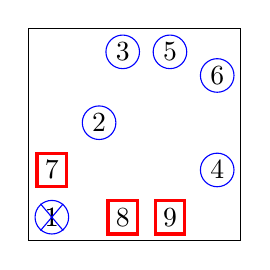
\begin{tikzpicture}[x = 3mm, y=3mm]
	\draw (-1,-1) rectangle (8,8);
	\tikzstyle{Square} = [
		draw = red, 
		very thick,
		rectangle,
		inner sep = 1mm,
		minimum size = 3 mm
	]
	\tikzstyle{SquareFill} = [
		draw = red, 
		fill = red,
		very thick,
		rectangle,
	]
	\tikzstyle{Circle} = [
		draw = blue, 
		circle,
		inner sep = 0.5 mm
	]
	\tikzstyle{CircleFill} = [
		draw = blue,
		fill = blue, 
		circle,
	]
	\node [Circle] (1) at (0,0) {1};
	\node [Circle] (2) at (2,4) {2};
	\node [Circle] (3) at (3,7) {3};
	\node [Circle] (4) at (7,2) {4};
	\node [Circle] (5) at (5,7) {5};
	\node [Circle] (6) at (7,6) {6};
	\node [Square] (7) at (0,2) {7};
	\node [Square] (8) at (3,0) {8};
	\node [Square] (9) at (5,0) {9};

	\node [Circle, cross out] (1) at (0,0) {1};
\end{tikzpicture}
\end{center}



Our original dataset has 619,027 samples.  We first removed the 27,723 crashes involving a pedestrian, leaving 591,304 samples.  Each sample had 82 features; we cut the number of features to 38 for our ``Hard'' features, then to 21 for ``Medium,'' and to 10 for ``Easy.''  We then split each of those three datasets 70/30 into a training set of 413,913 samples and a test set of 177,393 samples, preserving the proportions of negative and positive samples in both sets.  We did the train/test split twice with different random seeds (``Round 1'' and ``Round 2'') to gauge how much of the small differences in results were due to stochasticity instead of differences in the model algorithms or hyperparameters.  Tomek undersampling only applies to the training set, not to the test set.  

We then ran Imbalanced-Learn's  TomekLinks algorithm, then ran it again on the results to give our ``Tomek Once'' and ``Tomek Twice'' undersampled datasets.  

\

\hfil\begin{tabular}{lrrl}
\multicolumn{2}{l}{Hard Features, Round 1}   &  & \cr
 & Samples & \multicolumn{2}{c}{Change} \cr\hline
Original & 413,913 &  & \cr
Tomek Once & 399,515 & 14,398 & 3.48\%\cr
Tomek Twice & 396,511 & 3,004 & 0.75\%\cr\cline{3-4}
Total Change &  & 17,402 & 4.23\%\cr
\end{tabular}
\qquad\begin{tabular}{lrrl}
\multicolumn{2}{l}{Hard Features, Round 2} & \cr
 & Samples & \multicolumn{2}{c}{Change} \cr\hline
Original & 413,913 &  & \cr
Tomek Once & 399,714 & 14,199 & 3.43\%\cr
Tomek Twice & 396,718 & 2,996 & 0.75\%\cr\cline{3-4}
Total Change &  & 17,195 & 4.18\%\cr
\end{tabular}

\vskip 12pt

\hfil\begin{tabular}{lrrl}
\multicolumn{3}{l}{Medium Features, Round 1} & \cr
 & Samples & \multicolumn{2}{c}{Change} \cr\hline
Original & 413,913 &  & \cr
Tomek Once & 406,691 & 7,222 & 1.74\%\cr
Tomek Twice & 405,288 & 1,403 & 0.34\%\cr\cline{3-4}
Total Change &  & 8,625 & 2.08\%\cr
\end{tabular}
\qquad
\begin{tabular}{lrrl}
\multicolumn{3}{l}{Medium Features, Round 2} & \cr
 & Samples & \multicolumn{2}{c}{Change} \cr\hline
Original & 413,913 &  & \cr
Tomek Once & 406,781 & 7,132 & 1.72\%\cr
Tomek Twice & 405,368 & 1,413 & 0.35\%\cr\cline{3-4}
Total Change &  & 8,545 & 2.07\%\cr
\end{tabular}

\vskip 12pt

\hfil\begin{tabular}{lrrl}
\multicolumn{2}{l}{Easy Features, Round 1} & \cr
 & Samples & \multicolumn{2}{c}{Change} \cr\hline
Original & 413,913 &  & \cr
Tomek Once & 413,909 & 4 & 0.00097\%\cr
Tomek Twice & 413,908 & 1 & 0.00024\%\cr\cline{3-4}
Total Change &  & 5 & 0.00121\%\cr
\end{tabular}
\qquad
\begin{tabular}{lrrl}
\multicolumn{2}{l}{Easy Features, Round 2} & \cr
 & Samples & \multicolumn{2}{c}{Change} \cr\hline
Original & 413,913 &  & \cr
Tomek Once & 413,908 & 5 & 0.00121\%\cr
Tomek Twice & 413,907 & 1 & 0.00024\%\cr\cline{3-4}
Total Change &  & 6 & 0.00145\%\cr
\end{tabular}

\

We ran the models on the two rounds of Tomek undersampled training for the Hard-feature and Medium-feature sets, not for the Easy because the undersampling was so small.  

We were disappointed to not see a significant improvement in the model metrics from the undersampling; the difference between no undersampling, one runs of Tomek, and two runs turned out to be inconsequential, by which we mean that one approach was not consistently better when we ran the models with different random seeds.  


\subsubsection{Modifying the Loss Function}

A popular and well established way to modify the loss function for imbalanced data is with class weights, which can have the same effect as na{\"i}ve oversampling.  

Three of our seven models take class weights, and for those we tried three different class weights.  The Tomek undersampling changes the last weight slightly from $0.8499$ to as low as $0.8433$.

\

\hfil\begin{tabular}{c|l}
	$\alpha$ & Meaning \cr\hline
	1/2 & No class weight \cr
	2/3 & $\Delta FP/\Delta TP < 2.0$ goal \cr
	$0.85$ & Balanced classes \cr 
\end{tabular}

\


A related method is with focal loss, which has a modulating hyperparameter $\gamma$ that increases the penalty for low-confidence samples. \citep{lin2017focal}  We tried five values  of $\gamma$.

\

\hfil\begin{tabular}{c|c}
	$\gamma$  & Notes \cr\hline
	0.0 & Same as binary crossentropy \cr
	0.5 & Very light modulation \cr
	1.0 & Light modulation\cr
	2.0 & Recommended by Lin \cr
	5.0 & Heavy modulation \cr
\end{tabular}	

\

We did not see significant improvement using focal loss.  ({\bf Put in Label Reference}).

%%%
\subsubsection{Metrics for Imbalance}

In the \nameref{Methods_Metrics} subsection above we defined the metrics recall, precision, and f1.  The most common metric in machine learning, the one that most algorithms are designed to maximize, is accuracy, the proportion of samples correctly classified.  In that section's example of transformed model output, we had 150,107 out of 177,392 test samples correctly classified, giving 84.6\% accuracy.  Is that good?  The model below, the raw results of the Logistic Regression model of the easy features set, recommends sending no ambulances, and it is correct in 150,771 of 177,392 test samples, giving 84.99\% accuracy.  Is that better?



\

%%%
\parbox{\linewidth}{
%{\bf Balanced Random Forest model, Hard features, No Tomek, $\alpha = 2/3$}

\noindent\begin{tabular}{@{\hspace{-6pt}}p{2.3in} @{\hspace{-6pt}}p{2.0in} p{1.8in}}
	\vskip 0pt
	\qquad \qquad Raw Model Output
	
	\input{../Keras/Images/LRC_Easy_Tomek_0_alpha_0_5_v1_Pred.pgf}
&
	\vskip 0pt
	\qquad \qquad ROC Curve
	
	\input{../Keras/Images/LRC_Easy_Tomek_0_alpha_0_5_v1_ROC.pgf}
	
&
	\vskip 0pt
	\begin{tabular}{cc|c|c|}
	&\multicolumn{1}{c}{}& \multicolumn{2}{c}{Prediction} \cr
	&\multicolumn{1}{c}{} & \multicolumn{1}{c}{N} & \multicolumn{1}{c}{P} \cr\cline{3-4}
	\multirow{2}{*}{\rotatebox[origin=c]{90}{Actual}}&N &
150,771 & 0
	\vrule width 0pt height 10pt depth 2pt \cr\cline{3-4}
	&P & 
26621 & 0
	\vrule width 0pt height 10pt depth 2pt \cr\cline{3-4}
	\end{tabular}

	\hfil\begin{tabular}{ll}
	\cr
	0.8499 & Accuracy\cr
und & Precision \cr	0.0 & Recall \cr	und & F1 \cr	0.659 & AUC \cr
\end{tabular}

\cr
\end{tabular}
} % End parbox

\

In this study, we  have arbitrarily decided that we are willing to trade off up to two false positives to get one more true positive.  Once we moved our decision thresholds to the ethical tradeoff point, the accuracy only varied from 0.836 to 0.854.  The difference in accuracy tells us how many more (or fewer) false positives than true positives we have, with them being equal at 0.8499, and we get the same information from precision being less than, more than, or equal to 0.5.    Therefore, we are not going to consider accuracy in evaluating our models. 

%%%
\subsubsection{ML Algorithms for Imbalanced Data}

{\bf [Expand this subsubsection]}

\begin{itemize}
	\item Random Undersampling Composite Models
	\item Bagging
	\item Boosting
\end{itemize}

%%%%%
\subsection{Models}

We used seven binary classification algorithms.  Three of them take class weights.

\

\hfil\begin{tabular}{llc}
&& Class \cr
Model & Source & Weights \cr\hline
KerasClassifier with the Binary Focal Crossentropy loss function & Keras & Yes \cr
Balanced Random Forest Classifier & Imbalanced-Learn & Yes \cr
Balanced Bagging Classifier & Imbalanced-Learn & No \cr
RUSBoost Classifier & Imbalanced-Learn & No \cr
Easy Ensemble Classifier with AdaBoost Estimator & Imbalanced-Learn & No \cr
Logistic Regression Classifier & Scikit-Learn & Yes \cr
AdaBoost  Classifier & Scikit-Learn & No \cr
\end{tabular}

\


For the focal loss function, we tried seven different combinations of the hyperparameters $\alpha$ for class weights and $\gamma$ for penalty on badly misclassified samples.  For the random forest and bagging models we tried three values of $\alpha$.  Altogether we had seventeen model/hyperparameter combinations.  We learned each of the seven models on datasets with the easy, medium, and hard features, and on the hard features we tested with Tomek undersampling 0, 1, and 2 times, for a total of five datasets, giving eighty-five model/hyperparameter/dataset combinations.    We learned each of those sixty-five with two different random seeds, for a total of one hundred seventy results.  

\

\hfil\noindent\begin{tabular}{ccc}
	\multicolumn{3}{c}{Seventeen Models} \cr
	Model & $\alpha$ & $\gamma$ \cr\hline
	Focal & 1/2 & 0.0 \cr
	Focal & 2/3 & 0.0 \cr
	Focal & 2/3 & 0.5 \cr
	Focal & 2/3 & 1.0 \cr
	Focal & 2/3 & 2.0 \cr
	Focal & 2/3 & 5.0 \cr
	Focal & 0.85 & 0.0 \cr
	Random Forest & 1/2 & \cr
	Random Forest & 2/3 & \cr
	Random Forest & 0.85 & \cr
	Bagging && \cr
	RUSBoost && \cr
	Easy Ens && \cr
	Log Reg & 1/2 & \cr
	Log Reg & 2/3 & \cr
	Log Reg & 0.85 & \cr
	AdaBoost && \cr
\end{tabular}
\quad
$\times$
\quad
\begin{tabular}{cc}
	\multicolumn{2}{c}{Seven Datasets} \cr
	Features & Tomek \cr\hline
	Hard & None \cr
	Hard & Once \cr
	Hard & Twice \cr
	Medium & None \cr
	Medium & Once \cr
	Medium & Twice \cr
	Easy & None \cr
\end{tabular}
\quad
$\times$
\quad
\begin{tabular}{cc}
	Run twice with \cr
	different \cr
	random seeds \cr\hline
	Random seed 1 \cr
	Random seed 2
\end{tabular}
\quad 
$=$ 
\quad 
\begin{tabular}{c}
	238  \cr Sets of  \cr
	Results \cr
\end{tabular}









\subsection{Analysis of Results}\label{Analysis}
% Analysis of Results

Our ML algorithms assign to each sample (feature vector, crash person) a probability $p \in [0,1]$ that the person needs an ambulance.  The histogram below left shows the percentage of the dataset in each range of $p$, showing the percentages for the negative class (``Does not need an ambulance'') and the positive class (``Needs an ambulance'').  On the right, the Receiver Operating Characteristic (ROC) curve, and particularly the area under the curve (AUC), is a metric for how well the model separates the two classes, with $AUC=1.0$ being perfect and $AUC=0.5$ (the dashed line) being just random assignment with no insight.  

We would love to have results like in the graphs below, where the machine learning (ML) algorithm nearly perfectly separates the two classes.  There is some overlap between $p=0.6$ and $p=0.8$ with some samples the algorithm misclassifies, but the model clearly separates most samples.  Having an AUC of 0.996 would be amazing.  

[Put in \verb|BRFC_Hard_alpha_0_5_Train_Pred_Wide.pgf| once we have it.)

\begin{comment}

\noindent\begin{tabular}{@{\hspace{-6pt}}p{4.3in} @{\hspace{-6pt}}p{2.0in}}
	\vskip 0pt
	\hfil Raw Model Output
	
	\input{../Keras/Images/BRFC_Hard_Tomek_0_alpha_0_5_v1_Train_Pred_Wide.pgf}	
&
	\vskip 0pt
	\hfil ROC Curve
	
	\input{../Keras/Images/BRFC_Hard_Tomek_0_alpha_0_5_v1_Train_ROC.pgf}
	
\end{tabular}
\end{comment}

Unfortunately, our test results do not look quite that nice.  They do not separate the two classes as well.  Some distributions are clustered to one side or in the middle.  Some models give the results in $p \in [0,1]$ rounded to two decimal places so that we cannot hope for a level of detail beyond that, and one algorithm, Bagging, gives $p$ rounded to only one decimal place.  

Let us look at some examples.  In all of them, AUC is in the range $[0.7,0.8]$, so the various models separate the positive and negative classes about equally well overall, with none being dramatically better or worse.  We will later show how we investigated which models do a better job in the ranges of interest.  

\

%
\verb|BRFC_5_Fold_alpha_0_5_Hard_Test|

\

This model does not separate the negative and positive classes as well as the ideal, giving a much lower AUC (area under the ROC curve).  These results are actually from the same model as the ideal above, but the ideal are the results on the training set and below on the test set, showing overfitting.  

In these results, the 100 most frequent values comprised 93\% of the results, meaning that, while there is some noise making the distribution look continuous, it is mostly discrete to two decimal places, so we cannot hope for fine detail in tuning the decision threshold.  

\noindent\begin{tabular}{@{\hspace{-6pt}}p{4.3in} @{\hspace{-6pt}}p{2.0in}}
	\vskip 0pt
	\hfil Raw Model Output
	
	\input{../Keras/Images/BRFC_5_Fold_alpha_0_5_Hard_Test_Pred_Wide.pgf}	
&
	\vskip 0pt
	\hfil ROC Curve
	
	\input{../Keras/Images/BRFC_5_Fold_alpha_0_5_Hard_Test_ROC.pgf}
\end{tabular}

\

\

%
\verb|AdaBoost_5_Fold_Hard_Test|

\

In this model the values are clustered very tightly, but in that small range the 214,070 samples return 210,442 different values of $p$, so there is much diversity that we can't see in this representation.  


\

\verb|AdaBoost_5_Fold_Hard_Test|



\noindent\begin{tabular}{@{\hspace{-6pt}}p{4.3in} @{\hspace{-6pt}}p{2.0in}}
	\vskip 0pt
	\hfil Raw Model Output
	
	\input{../Keras/Images/AdaBoost_5_Fold_Hard_Test_Pred_Wide.pgf}	
&
	\vskip 0pt
	\hfil ROC Curve
	
	\input{../Keras/Images/AdaBoost_5_Fold_Hard_Test_ROC.pgf}
\end{tabular}


\

In this work we used two methods to give the results of different models similar distributions.  This case illustrates directly transforming the \verb|y_proba| values.  

To make a useful visualization of the results where we can see the interplay between the negative and positive classes, we can transform the data.  A transformation that preserves rank will have no effect on the ROC curve.  [Cite]  For the graph below, we mapped the smallest value in the set to 0 and the largest to 1.  

\

\verb|AdaBoost_5_Fold_Hard_Test_Transformed_100|

%
\noindent\begin{tabular}{@{\hspace{-6pt}}p{4.3in} @{\hspace{-6pt}}p{2.0in}}
	\vskip 0pt
	\hfil Raw Model Output
	
	\input{../Keras/Images/AdaBoost_5_Fold_Hard_Test_Transformed_100_Pred_Wide.pgf}	
&
	\vskip 0pt
	\hfil ROC Curve
	
	\input{../Keras/Images/AdaBoost_5_Fold_Hard_Test_Transformed_100_ROC.pgf}
\end{tabular}

The distribution has long tails, so we can make a more useful visualization by truncating the ends.  For this graph we mapped the 0.01 quantile to 0 and the 0.99 quantile to 1 leaving the center 98\% of the distribution and truncated the ends.  Our goal in clipping the tails is to make all of the models' results have approximately the same granularity when we choose the decision thresholds that give us the (politically) desired results.  


\

\verb|AdaBoost_5_Fold_Hard_Test_Transformed_98|

%
\noindent\begin{tabular}{@{\hspace{-6pt}}p{4.3in} @{\hspace{-6pt}}p{2.0in}}
	\vskip 0pt
	\hfil Raw Model Output
	
	\input{../Keras/Images/AdaBoost_5_Fold_Hard_Test_Transformed_98_Pred_Wide.pgf}	
&
	\vskip 0pt
	\hfil ROC Curve
	
	%% Creator: Matplotlib, PGF backend
%%
%% To include the figure in your LaTeX document, write
%%   \input{<filename>.pgf}
%%
%% Make sure the required packages are loaded in your preamble
%%   \usepackage{pgf}
%%
%% Also ensure that all the required font packages are loaded; for instance,
%% the lmodern package is sometimes necessary when using math font.
%%   \usepackage{lmodern}
%%
%% Figures using additional raster images can only be included by \input if
%% they are in the same directory as the main LaTeX file. For loading figures
%% from other directories you can use the `import` package
%%   \usepackage{import}
%%
%% and then include the figures with
%%   \import{<path to file>}{<filename>.pgf}
%%
%% Matplotlib used the following preamble
%%   
%%   \usepackage{fontspec}
%%   \makeatletter\@ifpackageloaded{underscore}{}{\usepackage[strings]{underscore}}\makeatother
%%
\begingroup%
\makeatletter%
\begin{pgfpicture}%
\pgfpathrectangle{\pgfpointorigin}{\pgfqpoint{2.221861in}{1.754444in}}%
\pgfusepath{use as bounding box, clip}%
\begin{pgfscope}%
\pgfsetbuttcap%
\pgfsetmiterjoin%
\definecolor{currentfill}{rgb}{1.000000,1.000000,1.000000}%
\pgfsetfillcolor{currentfill}%
\pgfsetlinewidth{0.000000pt}%
\definecolor{currentstroke}{rgb}{1.000000,1.000000,1.000000}%
\pgfsetstrokecolor{currentstroke}%
\pgfsetdash{}{0pt}%
\pgfpathmoveto{\pgfqpoint{0.000000in}{0.000000in}}%
\pgfpathlineto{\pgfqpoint{2.221861in}{0.000000in}}%
\pgfpathlineto{\pgfqpoint{2.221861in}{1.754444in}}%
\pgfpathlineto{\pgfqpoint{0.000000in}{1.754444in}}%
\pgfpathlineto{\pgfqpoint{0.000000in}{0.000000in}}%
\pgfpathclose%
\pgfusepath{fill}%
\end{pgfscope}%
\begin{pgfscope}%
\pgfsetbuttcap%
\pgfsetmiterjoin%
\definecolor{currentfill}{rgb}{1.000000,1.000000,1.000000}%
\pgfsetfillcolor{currentfill}%
\pgfsetlinewidth{0.000000pt}%
\definecolor{currentstroke}{rgb}{0.000000,0.000000,0.000000}%
\pgfsetstrokecolor{currentstroke}%
\pgfsetstrokeopacity{0.000000}%
\pgfsetdash{}{0pt}%
\pgfpathmoveto{\pgfqpoint{0.553581in}{0.499444in}}%
\pgfpathlineto{\pgfqpoint{2.103581in}{0.499444in}}%
\pgfpathlineto{\pgfqpoint{2.103581in}{1.654444in}}%
\pgfpathlineto{\pgfqpoint{0.553581in}{1.654444in}}%
\pgfpathlineto{\pgfqpoint{0.553581in}{0.499444in}}%
\pgfpathclose%
\pgfusepath{fill}%
\end{pgfscope}%
\begin{pgfscope}%
\pgfsetbuttcap%
\pgfsetroundjoin%
\definecolor{currentfill}{rgb}{0.000000,0.000000,0.000000}%
\pgfsetfillcolor{currentfill}%
\pgfsetlinewidth{0.803000pt}%
\definecolor{currentstroke}{rgb}{0.000000,0.000000,0.000000}%
\pgfsetstrokecolor{currentstroke}%
\pgfsetdash{}{0pt}%
\pgfsys@defobject{currentmarker}{\pgfqpoint{0.000000in}{-0.048611in}}{\pgfqpoint{0.000000in}{0.000000in}}{%
\pgfpathmoveto{\pgfqpoint{0.000000in}{0.000000in}}%
\pgfpathlineto{\pgfqpoint{0.000000in}{-0.048611in}}%
\pgfusepath{stroke,fill}%
}%
\begin{pgfscope}%
\pgfsys@transformshift{0.624035in}{0.499444in}%
\pgfsys@useobject{currentmarker}{}%
\end{pgfscope}%
\end{pgfscope}%
\begin{pgfscope}%
\definecolor{textcolor}{rgb}{0.000000,0.000000,0.000000}%
\pgfsetstrokecolor{textcolor}%
\pgfsetfillcolor{textcolor}%
\pgftext[x=0.624035in,y=0.402222in,,top]{\color{textcolor}\rmfamily\fontsize{10.000000}{12.000000}\selectfont \(\displaystyle {0.0}\)}%
\end{pgfscope}%
\begin{pgfscope}%
\pgfsetbuttcap%
\pgfsetroundjoin%
\definecolor{currentfill}{rgb}{0.000000,0.000000,0.000000}%
\pgfsetfillcolor{currentfill}%
\pgfsetlinewidth{0.803000pt}%
\definecolor{currentstroke}{rgb}{0.000000,0.000000,0.000000}%
\pgfsetstrokecolor{currentstroke}%
\pgfsetdash{}{0pt}%
\pgfsys@defobject{currentmarker}{\pgfqpoint{0.000000in}{-0.048611in}}{\pgfqpoint{0.000000in}{0.000000in}}{%
\pgfpathmoveto{\pgfqpoint{0.000000in}{0.000000in}}%
\pgfpathlineto{\pgfqpoint{0.000000in}{-0.048611in}}%
\pgfusepath{stroke,fill}%
}%
\begin{pgfscope}%
\pgfsys@transformshift{1.328581in}{0.499444in}%
\pgfsys@useobject{currentmarker}{}%
\end{pgfscope}%
\end{pgfscope}%
\begin{pgfscope}%
\definecolor{textcolor}{rgb}{0.000000,0.000000,0.000000}%
\pgfsetstrokecolor{textcolor}%
\pgfsetfillcolor{textcolor}%
\pgftext[x=1.328581in,y=0.402222in,,top]{\color{textcolor}\rmfamily\fontsize{10.000000}{12.000000}\selectfont \(\displaystyle {0.5}\)}%
\end{pgfscope}%
\begin{pgfscope}%
\pgfsetbuttcap%
\pgfsetroundjoin%
\definecolor{currentfill}{rgb}{0.000000,0.000000,0.000000}%
\pgfsetfillcolor{currentfill}%
\pgfsetlinewidth{0.803000pt}%
\definecolor{currentstroke}{rgb}{0.000000,0.000000,0.000000}%
\pgfsetstrokecolor{currentstroke}%
\pgfsetdash{}{0pt}%
\pgfsys@defobject{currentmarker}{\pgfqpoint{0.000000in}{-0.048611in}}{\pgfqpoint{0.000000in}{0.000000in}}{%
\pgfpathmoveto{\pgfqpoint{0.000000in}{0.000000in}}%
\pgfpathlineto{\pgfqpoint{0.000000in}{-0.048611in}}%
\pgfusepath{stroke,fill}%
}%
\begin{pgfscope}%
\pgfsys@transformshift{2.033126in}{0.499444in}%
\pgfsys@useobject{currentmarker}{}%
\end{pgfscope}%
\end{pgfscope}%
\begin{pgfscope}%
\definecolor{textcolor}{rgb}{0.000000,0.000000,0.000000}%
\pgfsetstrokecolor{textcolor}%
\pgfsetfillcolor{textcolor}%
\pgftext[x=2.033126in,y=0.402222in,,top]{\color{textcolor}\rmfamily\fontsize{10.000000}{12.000000}\selectfont \(\displaystyle {1.0}\)}%
\end{pgfscope}%
\begin{pgfscope}%
\definecolor{textcolor}{rgb}{0.000000,0.000000,0.000000}%
\pgfsetstrokecolor{textcolor}%
\pgfsetfillcolor{textcolor}%
\pgftext[x=1.328581in,y=0.223333in,,top]{\color{textcolor}\rmfamily\fontsize{10.000000}{12.000000}\selectfont False positive rate}%
\end{pgfscope}%
\begin{pgfscope}%
\pgfsetbuttcap%
\pgfsetroundjoin%
\definecolor{currentfill}{rgb}{0.000000,0.000000,0.000000}%
\pgfsetfillcolor{currentfill}%
\pgfsetlinewidth{0.803000pt}%
\definecolor{currentstroke}{rgb}{0.000000,0.000000,0.000000}%
\pgfsetstrokecolor{currentstroke}%
\pgfsetdash{}{0pt}%
\pgfsys@defobject{currentmarker}{\pgfqpoint{-0.048611in}{0.000000in}}{\pgfqpoint{-0.000000in}{0.000000in}}{%
\pgfpathmoveto{\pgfqpoint{-0.000000in}{0.000000in}}%
\pgfpathlineto{\pgfqpoint{-0.048611in}{0.000000in}}%
\pgfusepath{stroke,fill}%
}%
\begin{pgfscope}%
\pgfsys@transformshift{0.553581in}{0.551944in}%
\pgfsys@useobject{currentmarker}{}%
\end{pgfscope}%
\end{pgfscope}%
\begin{pgfscope}%
\definecolor{textcolor}{rgb}{0.000000,0.000000,0.000000}%
\pgfsetstrokecolor{textcolor}%
\pgfsetfillcolor{textcolor}%
\pgftext[x=0.278889in, y=0.503750in, left, base]{\color{textcolor}\rmfamily\fontsize{10.000000}{12.000000}\selectfont \(\displaystyle {0.0}\)}%
\end{pgfscope}%
\begin{pgfscope}%
\pgfsetbuttcap%
\pgfsetroundjoin%
\definecolor{currentfill}{rgb}{0.000000,0.000000,0.000000}%
\pgfsetfillcolor{currentfill}%
\pgfsetlinewidth{0.803000pt}%
\definecolor{currentstroke}{rgb}{0.000000,0.000000,0.000000}%
\pgfsetstrokecolor{currentstroke}%
\pgfsetdash{}{0pt}%
\pgfsys@defobject{currentmarker}{\pgfqpoint{-0.048611in}{0.000000in}}{\pgfqpoint{-0.000000in}{0.000000in}}{%
\pgfpathmoveto{\pgfqpoint{-0.000000in}{0.000000in}}%
\pgfpathlineto{\pgfqpoint{-0.048611in}{0.000000in}}%
\pgfusepath{stroke,fill}%
}%
\begin{pgfscope}%
\pgfsys@transformshift{0.553581in}{1.076944in}%
\pgfsys@useobject{currentmarker}{}%
\end{pgfscope}%
\end{pgfscope}%
\begin{pgfscope}%
\definecolor{textcolor}{rgb}{0.000000,0.000000,0.000000}%
\pgfsetstrokecolor{textcolor}%
\pgfsetfillcolor{textcolor}%
\pgftext[x=0.278889in, y=1.028750in, left, base]{\color{textcolor}\rmfamily\fontsize{10.000000}{12.000000}\selectfont \(\displaystyle {0.5}\)}%
\end{pgfscope}%
\begin{pgfscope}%
\pgfsetbuttcap%
\pgfsetroundjoin%
\definecolor{currentfill}{rgb}{0.000000,0.000000,0.000000}%
\pgfsetfillcolor{currentfill}%
\pgfsetlinewidth{0.803000pt}%
\definecolor{currentstroke}{rgb}{0.000000,0.000000,0.000000}%
\pgfsetstrokecolor{currentstroke}%
\pgfsetdash{}{0pt}%
\pgfsys@defobject{currentmarker}{\pgfqpoint{-0.048611in}{0.000000in}}{\pgfqpoint{-0.000000in}{0.000000in}}{%
\pgfpathmoveto{\pgfqpoint{-0.000000in}{0.000000in}}%
\pgfpathlineto{\pgfqpoint{-0.048611in}{0.000000in}}%
\pgfusepath{stroke,fill}%
}%
\begin{pgfscope}%
\pgfsys@transformshift{0.553581in}{1.601944in}%
\pgfsys@useobject{currentmarker}{}%
\end{pgfscope}%
\end{pgfscope}%
\begin{pgfscope}%
\definecolor{textcolor}{rgb}{0.000000,0.000000,0.000000}%
\pgfsetstrokecolor{textcolor}%
\pgfsetfillcolor{textcolor}%
\pgftext[x=0.278889in, y=1.553750in, left, base]{\color{textcolor}\rmfamily\fontsize{10.000000}{12.000000}\selectfont \(\displaystyle {1.0}\)}%
\end{pgfscope}%
\begin{pgfscope}%
\definecolor{textcolor}{rgb}{0.000000,0.000000,0.000000}%
\pgfsetstrokecolor{textcolor}%
\pgfsetfillcolor{textcolor}%
\pgftext[x=0.223333in,y=1.076944in,,bottom,rotate=90.000000]{\color{textcolor}\rmfamily\fontsize{10.000000}{12.000000}\selectfont True positive rate}%
\end{pgfscope}%
\begin{pgfscope}%
\pgfpathrectangle{\pgfqpoint{0.553581in}{0.499444in}}{\pgfqpoint{1.550000in}{1.155000in}}%
\pgfusepath{clip}%
\pgfsetbuttcap%
\pgfsetroundjoin%
\pgfsetlinewidth{1.505625pt}%
\definecolor{currentstroke}{rgb}{0.000000,0.000000,0.000000}%
\pgfsetstrokecolor{currentstroke}%
\pgfsetdash{{5.550000pt}{2.400000pt}}{0.000000pt}%
\pgfpathmoveto{\pgfqpoint{0.624035in}{0.551944in}}%
\pgfpathlineto{\pgfqpoint{2.033126in}{1.601944in}}%
\pgfusepath{stroke}%
\end{pgfscope}%
\begin{pgfscope}%
\pgfpathrectangle{\pgfqpoint{0.553581in}{0.499444in}}{\pgfqpoint{1.550000in}{1.155000in}}%
\pgfusepath{clip}%
\pgfsetrectcap%
\pgfsetroundjoin%
\pgfsetlinewidth{1.505625pt}%
\definecolor{currentstroke}{rgb}{0.000000,0.000000,0.000000}%
\pgfsetstrokecolor{currentstroke}%
\pgfsetdash{}{0pt}%
\pgfpathmoveto{\pgfqpoint{0.624035in}{0.551944in}}%
\pgfpathlineto{\pgfqpoint{0.628637in}{0.584231in}}%
\pgfpathlineto{\pgfqpoint{0.628843in}{0.585339in}}%
\pgfpathlineto{\pgfqpoint{0.629941in}{0.590703in}}%
\pgfpathlineto{\pgfqpoint{0.630194in}{0.591811in}}%
\pgfpathlineto{\pgfqpoint{0.631299in}{0.597846in}}%
\pgfpathlineto{\pgfqpoint{0.631477in}{0.598954in}}%
\pgfpathlineto{\pgfqpoint{0.632586in}{0.603629in}}%
\pgfpathlineto{\pgfqpoint{0.632823in}{0.604728in}}%
\pgfpathlineto{\pgfqpoint{0.633930in}{0.609757in}}%
\pgfpathlineto{\pgfqpoint{0.634275in}{0.610865in}}%
\pgfpathlineto{\pgfqpoint{0.635384in}{0.615502in}}%
\pgfpathlineto{\pgfqpoint{0.635652in}{0.616592in}}%
\pgfpathlineto{\pgfqpoint{0.636758in}{0.621099in}}%
\pgfpathlineto{\pgfqpoint{0.637059in}{0.622198in}}%
\pgfpathlineto{\pgfqpoint{0.638166in}{0.627115in}}%
\pgfpathlineto{\pgfqpoint{0.638424in}{0.628195in}}%
\pgfpathlineto{\pgfqpoint{0.639533in}{0.633075in}}%
\pgfpathlineto{\pgfqpoint{0.639852in}{0.634183in}}%
\pgfpathlineto{\pgfqpoint{0.640959in}{0.638765in}}%
\pgfpathlineto{\pgfqpoint{0.641341in}{0.639873in}}%
\pgfpathlineto{\pgfqpoint{0.642451in}{0.644679in}}%
\pgfpathlineto{\pgfqpoint{0.642694in}{0.645787in}}%
\pgfpathlineto{\pgfqpoint{0.643801in}{0.649707in}}%
\pgfpathlineto{\pgfqpoint{0.644174in}{0.650778in}}%
\pgfpathlineto{\pgfqpoint{0.645281in}{0.654820in}}%
\pgfpathlineto{\pgfqpoint{0.645586in}{0.655910in}}%
\pgfpathlineto{\pgfqpoint{0.646693in}{0.660398in}}%
\pgfpathlineto{\pgfqpoint{0.647014in}{0.661497in}}%
\pgfpathlineto{\pgfqpoint{0.648124in}{0.665259in}}%
\pgfpathlineto{\pgfqpoint{0.648485in}{0.666368in}}%
\pgfpathlineto{\pgfqpoint{0.649594in}{0.670130in}}%
\pgfpathlineto{\pgfqpoint{0.649909in}{0.671229in}}%
\pgfpathlineto{\pgfqpoint{0.651018in}{0.675429in}}%
\pgfpathlineto{\pgfqpoint{0.651339in}{0.676537in}}%
\pgfpathlineto{\pgfqpoint{0.652449in}{0.680541in}}%
\pgfpathlineto{\pgfqpoint{0.652742in}{0.681649in}}%
\pgfpathlineto{\pgfqpoint{0.653846in}{0.685365in}}%
\pgfpathlineto{\pgfqpoint{0.654156in}{0.686464in}}%
\pgfpathlineto{\pgfqpoint{0.655265in}{0.690496in}}%
\pgfpathlineto{\pgfqpoint{0.655617in}{0.691605in}}%
\pgfpathlineto{\pgfqpoint{0.656726in}{0.695460in}}%
\pgfpathlineto{\pgfqpoint{0.657167in}{0.696559in}}%
\pgfpathlineto{\pgfqpoint{0.658277in}{0.699744in}}%
\pgfpathlineto{\pgfqpoint{0.658598in}{0.700852in}}%
\pgfpathlineto{\pgfqpoint{0.659707in}{0.704568in}}%
\pgfpathlineto{\pgfqpoint{0.660014in}{0.705657in}}%
\pgfpathlineto{\pgfqpoint{0.661121in}{0.709094in}}%
\pgfpathlineto{\pgfqpoint{0.661384in}{0.710202in}}%
\pgfpathlineto{\pgfqpoint{0.662489in}{0.713880in}}%
\pgfpathlineto{\pgfqpoint{0.662493in}{0.713880in}}%
\pgfpathlineto{\pgfqpoint{0.662902in}{0.714988in}}%
\pgfpathlineto{\pgfqpoint{0.664011in}{0.718592in}}%
\pgfpathlineto{\pgfqpoint{0.664405in}{0.719691in}}%
\pgfpathlineto{\pgfqpoint{0.665512in}{0.723128in}}%
\pgfpathlineto{\pgfqpoint{0.665972in}{0.724236in}}%
\pgfpathlineto{\pgfqpoint{0.667081in}{0.727737in}}%
\pgfpathlineto{\pgfqpoint{0.667475in}{0.728845in}}%
\pgfpathlineto{\pgfqpoint{0.668584in}{0.732217in}}%
\pgfpathlineto{\pgfqpoint{0.668976in}{0.733325in}}%
\pgfpathlineto{\pgfqpoint{0.670083in}{0.736323in}}%
\pgfpathlineto{\pgfqpoint{0.670449in}{0.737432in}}%
\pgfpathlineto{\pgfqpoint{0.671549in}{0.740412in}}%
\pgfpathlineto{\pgfqpoint{0.671954in}{0.741520in}}%
\pgfpathlineto{\pgfqpoint{0.673050in}{0.744844in}}%
\pgfpathlineto{\pgfqpoint{0.673061in}{0.744844in}}%
\pgfpathlineto{\pgfqpoint{0.673516in}{0.745934in}}%
\pgfpathlineto{\pgfqpoint{0.674621in}{0.748961in}}%
\pgfpathlineto{\pgfqpoint{0.674961in}{0.750069in}}%
\pgfpathlineto{\pgfqpoint{0.676068in}{0.752658in}}%
\pgfpathlineto{\pgfqpoint{0.676464in}{0.753757in}}%
\pgfpathlineto{\pgfqpoint{0.677567in}{0.757137in}}%
\pgfpathlineto{\pgfqpoint{0.678022in}{0.758245in}}%
\pgfpathlineto{\pgfqpoint{0.679131in}{0.761095in}}%
\pgfpathlineto{\pgfqpoint{0.679546in}{0.762203in}}%
\pgfpathlineto{\pgfqpoint{0.683200in}{0.772177in}}%
\pgfpathlineto{\pgfqpoint{0.683704in}{0.773276in}}%
\pgfpathlineto{\pgfqpoint{0.684800in}{0.776116in}}%
\pgfpathlineto{\pgfqpoint{0.685304in}{0.777224in}}%
\pgfpathlineto{\pgfqpoint{0.686394in}{0.779776in}}%
\pgfpathlineto{\pgfqpoint{0.686896in}{0.780884in}}%
\pgfpathlineto{\pgfqpoint{0.687989in}{0.783631in}}%
\pgfpathlineto{\pgfqpoint{0.688416in}{0.784739in}}%
\pgfpathlineto{\pgfqpoint{0.689525in}{0.787459in}}%
\pgfpathlineto{\pgfqpoint{0.689971in}{0.788567in}}%
\pgfpathlineto{\pgfqpoint{0.691080in}{0.791119in}}%
\pgfpathlineto{\pgfqpoint{0.691556in}{0.792227in}}%
\pgfpathlineto{\pgfqpoint{0.692663in}{0.794937in}}%
\pgfpathlineto{\pgfqpoint{0.693207in}{0.796036in}}%
\pgfpathlineto{\pgfqpoint{0.694314in}{0.798764in}}%
\pgfpathlineto{\pgfqpoint{0.694737in}{0.799872in}}%
\pgfpathlineto{\pgfqpoint{0.695839in}{0.802480in}}%
\pgfpathlineto{\pgfqpoint{0.696317in}{0.803579in}}%
\pgfpathlineto{\pgfqpoint{0.697410in}{0.806298in}}%
\pgfpathlineto{\pgfqpoint{0.697961in}{0.807406in}}%
\pgfpathlineto{\pgfqpoint{0.699061in}{0.810098in}}%
\pgfpathlineto{\pgfqpoint{0.699577in}{0.811206in}}%
\pgfpathlineto{\pgfqpoint{0.700687in}{0.813795in}}%
\pgfpathlineto{\pgfqpoint{0.701158in}{0.814903in}}%
\pgfpathlineto{\pgfqpoint{0.702265in}{0.817268in}}%
\pgfpathlineto{\pgfqpoint{0.702734in}{0.818376in}}%
\pgfpathlineto{\pgfqpoint{0.703843in}{0.820472in}}%
\pgfpathlineto{\pgfqpoint{0.704411in}{0.821580in}}%
\pgfpathlineto{\pgfqpoint{0.705520in}{0.824197in}}%
\pgfpathlineto{\pgfqpoint{0.705973in}{0.825305in}}%
\pgfpathlineto{\pgfqpoint{0.707082in}{0.827708in}}%
\pgfpathlineto{\pgfqpoint{0.707467in}{0.828816in}}%
\pgfpathlineto{\pgfqpoint{0.708576in}{0.830976in}}%
\pgfpathlineto{\pgfqpoint{0.709043in}{0.832075in}}%
\pgfpathlineto{\pgfqpoint{0.710150in}{0.834673in}}%
\pgfpathlineto{\pgfqpoint{0.710657in}{0.835763in}}%
\pgfpathlineto{\pgfqpoint{0.711763in}{0.838343in}}%
\pgfpathlineto{\pgfqpoint{0.712202in}{0.839432in}}%
\pgfpathlineto{\pgfqpoint{0.713302in}{0.841788in}}%
\pgfpathlineto{\pgfqpoint{0.713830in}{0.842887in}}%
\pgfpathlineto{\pgfqpoint{0.714932in}{0.845457in}}%
\pgfpathlineto{\pgfqpoint{0.715481in}{0.846566in}}%
\pgfpathlineto{\pgfqpoint{0.716562in}{0.848558in}}%
\pgfpathlineto{\pgfqpoint{0.716569in}{0.848558in}}%
\pgfpathlineto{\pgfqpoint{0.717057in}{0.849657in}}%
\pgfpathlineto{\pgfqpoint{0.718161in}{0.852023in}}%
\pgfpathlineto{\pgfqpoint{0.718616in}{0.853122in}}%
\pgfpathlineto{\pgfqpoint{0.719723in}{0.855301in}}%
\pgfpathlineto{\pgfqpoint{0.720246in}{0.856390in}}%
\pgfpathlineto{\pgfqpoint{0.721346in}{0.858690in}}%
\pgfpathlineto{\pgfqpoint{0.721891in}{0.859789in}}%
\pgfpathlineto{\pgfqpoint{0.723000in}{0.862117in}}%
\pgfpathlineto{\pgfqpoint{0.723553in}{0.863207in}}%
\pgfpathlineto{\pgfqpoint{0.724658in}{0.865163in}}%
\pgfpathlineto{\pgfqpoint{0.725162in}{0.866262in}}%
\pgfpathlineto{\pgfqpoint{0.726269in}{0.868208in}}%
\pgfpathlineto{\pgfqpoint{0.726858in}{0.869307in}}%
\pgfpathlineto{\pgfqpoint{0.727960in}{0.871505in}}%
\pgfpathlineto{\pgfqpoint{0.728504in}{0.872603in}}%
\pgfpathlineto{\pgfqpoint{0.729602in}{0.874717in}}%
\pgfpathlineto{\pgfqpoint{0.730237in}{0.875826in}}%
\pgfpathlineto{\pgfqpoint{0.731340in}{0.878135in}}%
\pgfpathlineto{\pgfqpoint{0.731940in}{0.879243in}}%
\pgfpathlineto{\pgfqpoint{0.733049in}{0.881450in}}%
\pgfpathlineto{\pgfqpoint{0.733521in}{0.882549in}}%
\pgfpathlineto{\pgfqpoint{0.734630in}{0.884486in}}%
\pgfpathlineto{\pgfqpoint{0.735254in}{0.885594in}}%
\pgfpathlineto{\pgfqpoint{0.736361in}{0.887541in}}%
\pgfpathlineto{\pgfqpoint{0.736896in}{0.888621in}}%
\pgfpathlineto{\pgfqpoint{0.738005in}{0.890465in}}%
\pgfpathlineto{\pgfqpoint{0.738636in}{0.891573in}}%
\pgfpathlineto{\pgfqpoint{0.739738in}{0.893603in}}%
\pgfpathlineto{\pgfqpoint{0.740367in}{0.894711in}}%
\pgfpathlineto{\pgfqpoint{0.741467in}{0.896984in}}%
\pgfpathlineto{\pgfqpoint{0.742098in}{0.898092in}}%
\pgfpathlineto{\pgfqpoint{0.743202in}{0.900252in}}%
\pgfpathlineto{\pgfqpoint{0.743913in}{0.901351in}}%
\pgfpathlineto{\pgfqpoint{0.745022in}{0.903353in}}%
\pgfpathlineto{\pgfqpoint{0.745627in}{0.904462in}}%
\pgfpathlineto{\pgfqpoint{0.746706in}{0.906436in}}%
\pgfpathlineto{\pgfqpoint{0.746732in}{0.906436in}}%
\pgfpathlineto{\pgfqpoint{0.747410in}{0.907544in}}%
\pgfpathlineto{\pgfqpoint{0.748514in}{0.909546in}}%
\pgfpathlineto{\pgfqpoint{0.749098in}{0.910645in}}%
\pgfpathlineto{\pgfqpoint{0.750208in}{0.912610in}}%
\pgfpathlineto{\pgfqpoint{0.750829in}{0.913700in}}%
\pgfpathlineto{\pgfqpoint{0.751936in}{0.915627in}}%
\pgfpathlineto{\pgfqpoint{0.752628in}{0.916726in}}%
\pgfpathlineto{\pgfqpoint{0.753737in}{0.918281in}}%
\pgfpathlineto{\pgfqpoint{0.754382in}{0.919390in}}%
\pgfpathlineto{\pgfqpoint{0.755492in}{0.921429in}}%
\pgfpathlineto{\pgfqpoint{0.756176in}{0.922519in}}%
\pgfpathlineto{\pgfqpoint{0.757281in}{0.924391in}}%
\pgfpathlineto{\pgfqpoint{0.758001in}{0.925489in}}%
\pgfpathlineto{\pgfqpoint{0.759106in}{0.927743in}}%
\pgfpathlineto{\pgfqpoint{0.759868in}{0.928851in}}%
\pgfpathlineto{\pgfqpoint{0.760977in}{0.930947in}}%
\pgfpathlineto{\pgfqpoint{0.761657in}{0.932045in}}%
\pgfpathlineto{\pgfqpoint{0.762755in}{0.934113in}}%
\pgfpathlineto{\pgfqpoint{0.763294in}{0.935221in}}%
\pgfpathlineto{\pgfqpoint{0.764399in}{0.937056in}}%
\pgfpathlineto{\pgfqpoint{0.765039in}{0.938164in}}%
\pgfpathlineto{\pgfqpoint{0.766139in}{0.939803in}}%
\pgfpathlineto{\pgfqpoint{0.766149in}{0.939803in}}%
\pgfpathlineto{\pgfqpoint{0.766606in}{0.940911in}}%
\pgfpathlineto{\pgfqpoint{0.767715in}{0.942327in}}%
\pgfpathlineto{\pgfqpoint{0.768438in}{0.943435in}}%
\pgfpathlineto{\pgfqpoint{0.769545in}{0.945176in}}%
\pgfpathlineto{\pgfqpoint{0.770201in}{0.946266in}}%
\pgfpathlineto{\pgfqpoint{0.771308in}{0.948016in}}%
\pgfpathlineto{\pgfqpoint{0.771974in}{0.949115in}}%
\pgfpathlineto{\pgfqpoint{0.773084in}{0.950689in}}%
\pgfpathlineto{\pgfqpoint{0.773715in}{0.951788in}}%
\pgfpathlineto{\pgfqpoint{0.774824in}{0.953585in}}%
\pgfpathlineto{\pgfqpoint{0.775593in}{0.954675in}}%
\pgfpathlineto{\pgfqpoint{0.776695in}{0.956454in}}%
\pgfpathlineto{\pgfqpoint{0.777364in}{0.957553in}}%
\pgfpathlineto{\pgfqpoint{0.778473in}{0.959368in}}%
\pgfpathlineto{\pgfqpoint{0.779149in}{0.960477in}}%
\pgfpathlineto{\pgfqpoint{0.780256in}{0.962097in}}%
\pgfpathlineto{\pgfqpoint{0.780858in}{0.963205in}}%
\pgfpathlineto{\pgfqpoint{0.781951in}{0.964984in}}%
\pgfpathlineto{\pgfqpoint{0.782610in}{0.966092in}}%
\pgfpathlineto{\pgfqpoint{0.783720in}{0.967834in}}%
\pgfpathlineto{\pgfqpoint{0.784477in}{0.968942in}}%
\pgfpathlineto{\pgfqpoint{0.785584in}{0.970730in}}%
\pgfpathlineto{\pgfqpoint{0.786220in}{0.971838in}}%
\pgfpathlineto{\pgfqpoint{0.787329in}{0.973701in}}%
\pgfpathlineto{\pgfqpoint{0.788056in}{0.974809in}}%
\pgfpathlineto{\pgfqpoint{0.789165in}{0.976345in}}%
\pgfpathlineto{\pgfqpoint{0.789881in}{0.977453in}}%
\pgfpathlineto{\pgfqpoint{0.790985in}{0.978990in}}%
\pgfpathlineto{\pgfqpoint{0.791717in}{0.980089in}}%
\pgfpathlineto{\pgfqpoint{0.792826in}{0.981849in}}%
\pgfpathlineto{\pgfqpoint{0.793560in}{0.982957in}}%
\pgfpathlineto{\pgfqpoint{0.794665in}{0.984782in}}%
\pgfpathlineto{\pgfqpoint{0.795357in}{0.985881in}}%
\pgfpathlineto{\pgfqpoint{0.796464in}{0.987483in}}%
\pgfpathlineto{\pgfqpoint{0.797207in}{0.988591in}}%
\pgfpathlineto{\pgfqpoint{0.798312in}{0.990240in}}%
\pgfpathlineto{\pgfqpoint{0.799107in}{0.991348in}}%
\pgfpathlineto{\pgfqpoint{0.800216in}{0.993024in}}%
\pgfpathlineto{\pgfqpoint{0.800990in}{0.994132in}}%
\pgfpathlineto{\pgfqpoint{0.802093in}{0.995622in}}%
\pgfpathlineto{\pgfqpoint{0.802799in}{0.996703in}}%
\pgfpathlineto{\pgfqpoint{0.803899in}{0.998397in}}%
\pgfpathlineto{\pgfqpoint{0.804715in}{0.999506in}}%
\pgfpathlineto{\pgfqpoint{0.805817in}{1.001107in}}%
\pgfpathlineto{\pgfqpoint{0.806765in}{1.002216in}}%
\pgfpathlineto{\pgfqpoint{0.807874in}{1.003780in}}%
\pgfpathlineto{\pgfqpoint{0.808622in}{1.004879in}}%
\pgfpathlineto{\pgfqpoint{0.809731in}{1.006350in}}%
\pgfpathlineto{\pgfqpoint{0.810512in}{1.007459in}}%
\pgfpathlineto{\pgfqpoint{0.811622in}{1.008976in}}%
\pgfpathlineto{\pgfqpoint{0.812522in}{1.010085in}}%
\pgfpathlineto{\pgfqpoint{0.813632in}{1.011351in}}%
\pgfpathlineto{\pgfqpoint{0.814485in}{1.012459in}}%
\pgfpathlineto{\pgfqpoint{0.815581in}{1.014061in}}%
\pgfpathlineto{\pgfqpoint{0.816406in}{1.015169in}}%
\pgfpathlineto{\pgfqpoint{0.817499in}{1.016920in}}%
\pgfpathlineto{\pgfqpoint{0.818371in}{1.018028in}}%
\pgfpathlineto{\pgfqpoint{0.819478in}{1.019304in}}%
\pgfpathlineto{\pgfqpoint{0.820325in}{1.020412in}}%
\pgfpathlineto{\pgfqpoint{0.821434in}{1.022182in}}%
\pgfpathlineto{\pgfqpoint{0.822405in}{1.023290in}}%
\pgfpathlineto{\pgfqpoint{0.823515in}{1.024743in}}%
\pgfpathlineto{\pgfqpoint{0.824289in}{1.025851in}}%
\pgfpathlineto{\pgfqpoint{0.825396in}{1.027294in}}%
\pgfpathlineto{\pgfqpoint{0.826212in}{1.028402in}}%
\pgfpathlineto{\pgfqpoint{0.827319in}{1.029809in}}%
\pgfpathlineto{\pgfqpoint{0.828184in}{1.030917in}}%
\pgfpathlineto{\pgfqpoint{0.829282in}{1.032528in}}%
\pgfpathlineto{\pgfqpoint{0.830018in}{1.033627in}}%
\pgfpathlineto{\pgfqpoint{0.831125in}{1.035294in}}%
\pgfpathlineto{\pgfqpoint{0.831946in}{1.036393in}}%
\pgfpathlineto{\pgfqpoint{0.833046in}{1.037873in}}%
\pgfpathlineto{\pgfqpoint{0.834000in}{1.038982in}}%
\pgfpathlineto{\pgfqpoint{0.835105in}{1.040388in}}%
\pgfpathlineto{\pgfqpoint{0.835879in}{1.041468in}}%
\pgfpathlineto{\pgfqpoint{0.836986in}{1.042753in}}%
\pgfpathlineto{\pgfqpoint{0.837870in}{1.043852in}}%
\pgfpathlineto{\pgfqpoint{0.838970in}{1.045240in}}%
\pgfpathlineto{\pgfqpoint{0.839807in}{1.046348in}}%
\pgfpathlineto{\pgfqpoint{0.840917in}{1.047717in}}%
\pgfpathlineto{\pgfqpoint{0.841740in}{1.048825in}}%
\pgfpathlineto{\pgfqpoint{0.842845in}{1.049905in}}%
\pgfpathlineto{\pgfqpoint{0.843785in}{1.051004in}}%
\pgfpathlineto{\pgfqpoint{0.844883in}{1.052503in}}%
\pgfpathlineto{\pgfqpoint{0.845811in}{1.053612in}}%
\pgfpathlineto{\pgfqpoint{0.846904in}{1.055334in}}%
\pgfpathlineto{\pgfqpoint{0.847847in}{1.056433in}}%
\pgfpathlineto{\pgfqpoint{0.848952in}{1.057923in}}%
\pgfpathlineto{\pgfqpoint{0.849876in}{1.059031in}}%
\pgfpathlineto{\pgfqpoint{0.850980in}{1.060289in}}%
\pgfpathlineto{\pgfqpoint{0.851776in}{1.061397in}}%
\pgfpathlineto{\pgfqpoint{0.852873in}{1.062905in}}%
\pgfpathlineto{\pgfqpoint{0.853839in}{1.064004in}}%
\pgfpathlineto{\pgfqpoint{0.854949in}{1.065606in}}%
\pgfpathlineto{\pgfqpoint{0.855920in}{1.066714in}}%
\pgfpathlineto{\pgfqpoint{0.857015in}{1.068139in}}%
\pgfpathlineto{\pgfqpoint{0.857883in}{1.069238in}}%
\pgfpathlineto{\pgfqpoint{0.858980in}{1.070830in}}%
\pgfpathlineto{\pgfqpoint{0.859871in}{1.071939in}}%
\pgfpathlineto{\pgfqpoint{0.860981in}{1.073475in}}%
\pgfpathlineto{\pgfqpoint{0.862095in}{1.074574in}}%
\pgfpathlineto{\pgfqpoint{0.863195in}{1.075897in}}%
\pgfpathlineto{\pgfqpoint{0.864156in}{1.077005in}}%
\pgfpathlineto{\pgfqpoint{0.865266in}{1.078364in}}%
\pgfpathlineto{\pgfqpoint{0.866023in}{1.079473in}}%
\pgfpathlineto{\pgfqpoint{0.867133in}{1.080814in}}%
\pgfpathlineto{\pgfqpoint{0.868186in}{1.081922in}}%
\pgfpathlineto{\pgfqpoint{0.869288in}{1.083123in}}%
\pgfpathlineto{\pgfqpoint{0.870242in}{1.084222in}}%
\pgfpathlineto{\pgfqpoint{0.871349in}{1.085805in}}%
\pgfpathlineto{\pgfqpoint{0.872290in}{1.086895in}}%
\pgfpathlineto{\pgfqpoint{0.873397in}{1.088347in}}%
\pgfpathlineto{\pgfqpoint{0.874377in}{1.089456in}}%
\pgfpathlineto{\pgfqpoint{0.875435in}{1.090862in}}%
\pgfpathlineto{\pgfqpoint{0.876418in}{1.091970in}}%
\pgfpathlineto{\pgfqpoint{0.877499in}{1.093078in}}%
\pgfpathlineto{\pgfqpoint{0.878578in}{1.094186in}}%
\pgfpathlineto{\pgfqpoint{0.879687in}{1.095341in}}%
\pgfpathlineto{\pgfqpoint{0.880559in}{1.096449in}}%
\pgfpathlineto{\pgfqpoint{0.881659in}{1.097623in}}%
\pgfpathlineto{\pgfqpoint{0.881669in}{1.097623in}}%
\pgfpathlineto{\pgfqpoint{0.882680in}{1.098731in}}%
\pgfpathlineto{\pgfqpoint{0.883768in}{1.100016in}}%
\pgfpathlineto{\pgfqpoint{0.883784in}{1.100016in}}%
\pgfpathlineto{\pgfqpoint{0.884659in}{1.101115in}}%
\pgfpathlineto{\pgfqpoint{0.885745in}{1.102512in}}%
\pgfpathlineto{\pgfqpoint{0.886889in}{1.103620in}}%
\pgfpathlineto{\pgfqpoint{0.887987in}{1.104840in}}%
\pgfpathlineto{\pgfqpoint{0.889052in}{1.105948in}}%
\pgfpathlineto{\pgfqpoint{0.890147in}{1.106945in}}%
\pgfpathlineto{\pgfqpoint{0.891144in}{1.108043in}}%
\pgfpathlineto{\pgfqpoint{0.892239in}{1.109366in}}%
\pgfpathlineto{\pgfqpoint{0.893177in}{1.110474in}}%
\pgfpathlineto{\pgfqpoint{0.894270in}{1.111694in}}%
\pgfpathlineto{\pgfqpoint{0.895241in}{1.112802in}}%
\pgfpathlineto{\pgfqpoint{0.896350in}{1.114013in}}%
\pgfpathlineto{\pgfqpoint{0.897302in}{1.115121in}}%
\pgfpathlineto{\pgfqpoint{0.898409in}{1.116415in}}%
\pgfpathlineto{\pgfqpoint{0.899409in}{1.117514in}}%
\pgfpathlineto{\pgfqpoint{0.900513in}{1.118809in}}%
\pgfpathlineto{\pgfqpoint{0.901522in}{1.119908in}}%
\pgfpathlineto{\pgfqpoint{0.902612in}{1.121323in}}%
\pgfpathlineto{\pgfqpoint{0.903787in}{1.122431in}}%
\pgfpathlineto{\pgfqpoint{0.904875in}{1.123782in}}%
\pgfpathlineto{\pgfqpoint{0.906090in}{1.124890in}}%
\pgfpathlineto{\pgfqpoint{0.907179in}{1.126249in}}%
\pgfpathlineto{\pgfqpoint{0.908023in}{1.127348in}}%
\pgfpathlineto{\pgfqpoint{0.909120in}{1.128568in}}%
\pgfpathlineto{\pgfqpoint{0.909130in}{1.128568in}}%
\pgfpathlineto{\pgfqpoint{0.910298in}{1.129667in}}%
\pgfpathlineto{\pgfqpoint{0.911402in}{1.131055in}}%
\pgfpathlineto{\pgfqpoint{0.912502in}{1.132163in}}%
\pgfpathlineto{\pgfqpoint{0.913602in}{1.133355in}}%
\pgfpathlineto{\pgfqpoint{0.913612in}{1.133355in}}%
\pgfpathlineto{\pgfqpoint{0.914700in}{1.134463in}}%
\pgfpathlineto{\pgfqpoint{0.915807in}{1.135664in}}%
\pgfpathlineto{\pgfqpoint{0.916862in}{1.136773in}}%
\pgfpathlineto{\pgfqpoint{0.917967in}{1.137704in}}%
\pgfpathlineto{\pgfqpoint{0.918900in}{1.138812in}}%
\pgfpathlineto{\pgfqpoint{0.920010in}{1.140051in}}%
\pgfpathlineto{\pgfqpoint{0.921035in}{1.141159in}}%
\pgfpathlineto{\pgfqpoint{0.922144in}{1.142183in}}%
\pgfpathlineto{\pgfqpoint{0.923335in}{1.143291in}}%
\pgfpathlineto{\pgfqpoint{0.924445in}{1.144558in}}%
\pgfpathlineto{\pgfqpoint{0.925636in}{1.145666in}}%
\pgfpathlineto{\pgfqpoint{0.926743in}{1.146663in}}%
\pgfpathlineto{\pgfqpoint{0.927770in}{1.147771in}}%
\pgfpathlineto{\pgfqpoint{0.928873in}{1.148860in}}%
\pgfpathlineto{\pgfqpoint{0.929832in}{1.149969in}}%
\pgfpathlineto{\pgfqpoint{0.930918in}{1.151067in}}%
\pgfpathlineto{\pgfqpoint{0.930932in}{1.151067in}}%
\pgfpathlineto{\pgfqpoint{0.932069in}{1.152176in}}%
\pgfpathlineto{\pgfqpoint{0.933171in}{1.153368in}}%
\pgfpathlineto{\pgfqpoint{0.933179in}{1.153368in}}%
\pgfpathlineto{\pgfqpoint{0.934215in}{1.154457in}}%
\pgfpathlineto{\pgfqpoint{0.935313in}{1.155714in}}%
\pgfpathlineto{\pgfqpoint{0.936438in}{1.156823in}}%
\pgfpathlineto{\pgfqpoint{0.937545in}{1.157968in}}%
\pgfpathlineto{\pgfqpoint{0.938643in}{1.159058in}}%
\pgfpathlineto{\pgfqpoint{0.938643in}{1.159067in}}%
\pgfpathlineto{\pgfqpoint{0.939750in}{1.160333in}}%
\pgfpathlineto{\pgfqpoint{0.940754in}{1.161442in}}%
\pgfpathlineto{\pgfqpoint{0.941842in}{1.162503in}}%
\pgfpathlineto{\pgfqpoint{0.942914in}{1.163602in}}%
\pgfpathlineto{\pgfqpoint{0.944014in}{1.164701in}}%
\pgfpathlineto{\pgfqpoint{0.945449in}{1.165809in}}%
\pgfpathlineto{\pgfqpoint{0.946558in}{1.166703in}}%
\pgfpathlineto{\pgfqpoint{0.947783in}{1.167811in}}%
\pgfpathlineto{\pgfqpoint{0.948890in}{1.168854in}}%
\pgfpathlineto{\pgfqpoint{0.950004in}{1.169963in}}%
\pgfpathlineto{\pgfqpoint{0.951104in}{1.170903in}}%
\pgfpathlineto{\pgfqpoint{0.952368in}{1.171974in}}%
\pgfpathlineto{\pgfqpoint{0.953475in}{1.173036in}}%
\pgfpathlineto{\pgfqpoint{0.954633in}{1.174144in}}%
\pgfpathlineto{\pgfqpoint{0.955712in}{1.175224in}}%
\pgfpathlineto{\pgfqpoint{0.956887in}{1.176323in}}%
\pgfpathlineto{\pgfqpoint{0.957996in}{1.177655in}}%
\pgfpathlineto{\pgfqpoint{0.958986in}{1.178763in}}%
\pgfpathlineto{\pgfqpoint{0.960067in}{1.179862in}}%
\pgfpathlineto{\pgfqpoint{0.961310in}{1.180970in}}%
\pgfpathlineto{\pgfqpoint{0.962415in}{1.182106in}}%
\pgfpathlineto{\pgfqpoint{0.963503in}{1.183214in}}%
\pgfpathlineto{\pgfqpoint{0.964613in}{1.184434in}}%
\pgfpathlineto{\pgfqpoint{0.965818in}{1.185543in}}%
\pgfpathlineto{\pgfqpoint{0.966918in}{1.186632in}}%
\pgfpathlineto{\pgfqpoint{0.967955in}{1.187740in}}%
\pgfpathlineto{\pgfqpoint{0.969052in}{1.188737in}}%
\pgfpathlineto{\pgfqpoint{0.970276in}{1.189845in}}%
\pgfpathlineto{\pgfqpoint{0.971372in}{1.190767in}}%
\pgfpathlineto{\pgfqpoint{0.972720in}{1.191875in}}%
\pgfpathlineto{\pgfqpoint{0.973827in}{1.192955in}}%
\pgfpathlineto{\pgfqpoint{0.975105in}{1.194064in}}%
\pgfpathlineto{\pgfqpoint{0.976212in}{1.195293in}}%
\pgfpathlineto{\pgfqpoint{0.977720in}{1.196401in}}%
\pgfpathlineto{\pgfqpoint{0.979203in}{1.197779in}}%
\pgfpathlineto{\pgfqpoint{0.980589in}{1.198887in}}%
\pgfpathlineto{\pgfqpoint{0.981698in}{1.199996in}}%
\pgfpathlineto{\pgfqpoint{0.982857in}{1.201095in}}%
\pgfpathlineto{\pgfqpoint{0.983964in}{1.202287in}}%
\pgfpathlineto{\pgfqpoint{0.985319in}{1.203385in}}%
\pgfpathlineto{\pgfqpoint{0.986410in}{1.204242in}}%
\pgfpathlineto{\pgfqpoint{0.987730in}{1.205350in}}%
\pgfpathlineto{\pgfqpoint{0.988837in}{1.206300in}}%
\pgfpathlineto{\pgfqpoint{0.990017in}{1.207408in}}%
\pgfpathlineto{\pgfqpoint{0.991089in}{1.208144in}}%
\pgfpathlineto{\pgfqpoint{0.992522in}{1.209252in}}%
\pgfpathlineto{\pgfqpoint{0.993631in}{1.210277in}}%
\pgfpathlineto{\pgfqpoint{0.995038in}{1.211385in}}%
\pgfpathlineto{\pgfqpoint{0.996147in}{1.212512in}}%
\pgfpathlineto{\pgfqpoint{0.997440in}{1.213611in}}%
\pgfpathlineto{\pgfqpoint{0.998542in}{1.214607in}}%
\pgfpathlineto{\pgfqpoint{0.999853in}{1.215715in}}%
\pgfpathlineto{\pgfqpoint{1.000962in}{1.216646in}}%
\pgfpathlineto{\pgfqpoint{1.002161in}{1.217755in}}%
\pgfpathlineto{\pgfqpoint{1.003270in}{1.218472in}}%
\pgfpathlineto{\pgfqpoint{1.004337in}{1.219580in}}%
\pgfpathlineto{\pgfqpoint{1.005432in}{1.220688in}}%
\pgfpathlineto{\pgfqpoint{1.006406in}{1.221796in}}%
\pgfpathlineto{\pgfqpoint{1.007513in}{1.222858in}}%
\pgfpathlineto{\pgfqpoint{1.008721in}{1.223966in}}%
\pgfpathlineto{\pgfqpoint{1.009825in}{1.225000in}}%
\pgfpathlineto{\pgfqpoint{1.011289in}{1.226108in}}%
\pgfpathlineto{\pgfqpoint{1.012384in}{1.227170in}}%
\pgfpathlineto{\pgfqpoint{1.013920in}{1.228259in}}%
\pgfpathlineto{\pgfqpoint{1.015027in}{1.229470in}}%
\pgfpathlineto{\pgfqpoint{1.016392in}{1.230569in}}%
\pgfpathlineto{\pgfqpoint{1.017494in}{1.231584in}}%
\pgfpathlineto{\pgfqpoint{1.018883in}{1.232692in}}%
\pgfpathlineto{\pgfqpoint{1.019966in}{1.233558in}}%
\pgfpathlineto{\pgfqpoint{1.021383in}{1.234666in}}%
\pgfpathlineto{\pgfqpoint{1.022487in}{1.235728in}}%
\pgfpathlineto{\pgfqpoint{1.023784in}{1.236836in}}%
\pgfpathlineto{\pgfqpoint{1.024873in}{1.237488in}}%
\pgfpathlineto{\pgfqpoint{1.026188in}{1.238596in}}%
\pgfpathlineto{\pgfqpoint{1.027286in}{1.239378in}}%
\pgfpathlineto{\pgfqpoint{1.028834in}{1.240487in}}%
\pgfpathlineto{\pgfqpoint{1.029936in}{1.241446in}}%
\pgfpathlineto{\pgfqpoint{1.031313in}{1.242554in}}%
\pgfpathlineto{\pgfqpoint{1.032378in}{1.243383in}}%
\pgfpathlineto{\pgfqpoint{1.033904in}{1.244491in}}%
\pgfpathlineto{\pgfqpoint{1.035011in}{1.245487in}}%
\pgfpathlineto{\pgfqpoint{1.036322in}{1.246596in}}%
\pgfpathlineto{\pgfqpoint{1.037420in}{1.247518in}}%
\pgfpathlineto{\pgfqpoint{1.038954in}{1.248626in}}%
\pgfpathlineto{\pgfqpoint{1.040063in}{1.249687in}}%
\pgfpathlineto{\pgfqpoint{1.041280in}{1.250786in}}%
\pgfpathlineto{\pgfqpoint{1.042369in}{1.251745in}}%
\pgfpathlineto{\pgfqpoint{1.043682in}{1.252854in}}%
\pgfpathlineto{\pgfqpoint{1.044787in}{1.253766in}}%
\pgfpathlineto{\pgfqpoint{1.046128in}{1.254875in}}%
\pgfpathlineto{\pgfqpoint{1.047212in}{1.255703in}}%
\pgfpathlineto{\pgfqpoint{1.048642in}{1.256812in}}%
\pgfpathlineto{\pgfqpoint{1.049747in}{1.257706in}}%
\pgfpathlineto{\pgfqpoint{1.051006in}{1.258814in}}%
\pgfpathlineto{\pgfqpoint{1.052102in}{1.259708in}}%
\pgfpathlineto{\pgfqpoint{1.053657in}{1.260816in}}%
\pgfpathlineto{\pgfqpoint{1.054747in}{1.261915in}}%
\pgfpathlineto{\pgfqpoint{1.056464in}{1.263023in}}%
\pgfpathlineto{\pgfqpoint{1.057568in}{1.263936in}}%
\pgfpathlineto{\pgfqpoint{1.059039in}{1.265044in}}%
\pgfpathlineto{\pgfqpoint{1.060148in}{1.265863in}}%
\pgfpathlineto{\pgfqpoint{1.061731in}{1.266972in}}%
\pgfpathlineto{\pgfqpoint{1.062838in}{1.267856in}}%
\pgfpathlineto{\pgfqpoint{1.064351in}{1.268964in}}%
\pgfpathlineto{\pgfqpoint{1.065458in}{1.269803in}}%
\pgfpathlineto{\pgfqpoint{1.066771in}{1.270892in}}%
\pgfpathlineto{\pgfqpoint{1.067867in}{1.271758in}}%
\pgfpathlineto{\pgfqpoint{1.067881in}{1.271758in}}%
\pgfpathlineto{\pgfqpoint{1.069408in}{1.272866in}}%
\pgfpathlineto{\pgfqpoint{1.070505in}{1.273695in}}%
\pgfpathlineto{\pgfqpoint{1.071884in}{1.274785in}}%
\pgfpathlineto{\pgfqpoint{1.072991in}{1.275725in}}%
\pgfpathlineto{\pgfqpoint{1.074276in}{1.276834in}}%
\pgfpathlineto{\pgfqpoint{1.075379in}{1.277700in}}%
\pgfpathlineto{\pgfqpoint{1.076842in}{1.278808in}}%
\pgfpathlineto{\pgfqpoint{1.077951in}{1.279609in}}%
\pgfpathlineto{\pgfqpoint{1.079598in}{1.280717in}}%
\pgfpathlineto{\pgfqpoint{1.080707in}{1.281508in}}%
\pgfpathlineto{\pgfqpoint{1.081863in}{1.282617in}}%
\pgfpathlineto{\pgfqpoint{1.082956in}{1.283539in}}%
\pgfpathlineto{\pgfqpoint{1.084448in}{1.284647in}}%
\pgfpathlineto{\pgfqpoint{1.085522in}{1.285280in}}%
\pgfpathlineto{\pgfqpoint{1.086929in}{1.286388in}}%
\pgfpathlineto{\pgfqpoint{1.088039in}{1.287273in}}%
\pgfpathlineto{\pgfqpoint{1.089615in}{1.288381in}}%
\pgfpathlineto{\pgfqpoint{1.090710in}{1.289154in}}%
\pgfpathlineto{\pgfqpoint{1.092162in}{1.290262in}}%
\pgfpathlineto{\pgfqpoint{1.093240in}{1.291091in}}%
\pgfpathlineto{\pgfqpoint{1.093271in}{1.291091in}}%
\pgfpathlineto{\pgfqpoint{1.094906in}{1.292199in}}%
\pgfpathlineto{\pgfqpoint{1.096003in}{1.292972in}}%
\pgfpathlineto{\pgfqpoint{1.097697in}{1.294080in}}%
\pgfpathlineto{\pgfqpoint{1.098796in}{1.294751in}}%
\pgfpathlineto{\pgfqpoint{1.100328in}{1.295859in}}%
\pgfpathlineto{\pgfqpoint{1.101426in}{1.296595in}}%
\pgfpathlineto{\pgfqpoint{1.102908in}{1.297703in}}%
\pgfpathlineto{\pgfqpoint{1.104012in}{1.298476in}}%
\pgfpathlineto{\pgfqpoint{1.105596in}{1.299584in}}%
\pgfpathlineto{\pgfqpoint{1.106686in}{1.300301in}}%
\pgfpathlineto{\pgfqpoint{1.108147in}{1.301409in}}%
\pgfpathlineto{\pgfqpoint{1.109254in}{1.302136in}}%
\pgfpathlineto{\pgfqpoint{1.110999in}{1.303244in}}%
\pgfpathlineto{\pgfqpoint{1.112106in}{1.304110in}}%
\pgfpathlineto{\pgfqpoint{1.113574in}{1.305218in}}%
\pgfpathlineto{\pgfqpoint{1.114679in}{1.306094in}}%
\pgfpathlineto{\pgfqpoint{1.116255in}{1.307202in}}%
\pgfpathlineto{\pgfqpoint{1.117357in}{1.307919in}}%
\pgfpathlineto{\pgfqpoint{1.119184in}{1.309027in}}%
\pgfpathlineto{\pgfqpoint{1.120270in}{1.309912in}}%
\pgfpathlineto{\pgfqpoint{1.121938in}{1.311020in}}%
\pgfpathlineto{\pgfqpoint{1.123026in}{1.311746in}}%
\pgfpathlineto{\pgfqpoint{1.124822in}{1.312854in}}%
\pgfpathlineto{\pgfqpoint{1.125925in}{1.313655in}}%
\pgfpathlineto{\pgfqpoint{1.127533in}{1.314764in}}%
\pgfpathlineto{\pgfqpoint{1.128608in}{1.315453in}}%
\pgfpathlineto{\pgfqpoint{1.130195in}{1.316561in}}%
\pgfpathlineto{\pgfqpoint{1.131300in}{1.317259in}}%
\pgfpathlineto{\pgfqpoint{1.133207in}{1.318368in}}%
\pgfpathlineto{\pgfqpoint{1.134316in}{1.319038in}}%
\pgfpathlineto{\pgfqpoint{1.136131in}{1.320137in}}%
\pgfpathlineto{\pgfqpoint{1.137236in}{1.320938in}}%
\pgfpathlineto{\pgfqpoint{1.138983in}{1.322046in}}%
\pgfpathlineto{\pgfqpoint{1.140081in}{1.322893in}}%
\pgfpathlineto{\pgfqpoint{1.140088in}{1.322893in}}%
\pgfpathlineto{\pgfqpoint{1.141854in}{1.324002in}}%
\pgfpathlineto{\pgfqpoint{1.142930in}{1.324784in}}%
\pgfpathlineto{\pgfqpoint{1.144403in}{1.325892in}}%
\pgfpathlineto{\pgfqpoint{1.145503in}{1.326674in}}%
\pgfpathlineto{\pgfqpoint{1.145508in}{1.326674in}}%
\pgfpathlineto{\pgfqpoint{1.147304in}{1.327773in}}%
\pgfpathlineto{\pgfqpoint{1.148407in}{1.328481in}}%
\pgfpathlineto{\pgfqpoint{1.150140in}{1.329589in}}%
\pgfpathlineto{\pgfqpoint{1.151240in}{1.330483in}}%
\pgfpathlineto{\pgfqpoint{1.152935in}{1.331591in}}%
\pgfpathlineto{\pgfqpoint{1.153979in}{1.332411in}}%
\pgfpathlineto{\pgfqpoint{1.153993in}{1.332411in}}%
\pgfpathlineto{\pgfqpoint{1.155654in}{1.333519in}}%
\pgfpathlineto{\pgfqpoint{1.156754in}{1.334301in}}%
\pgfpathlineto{\pgfqpoint{1.158688in}{1.335410in}}%
\pgfpathlineto{\pgfqpoint{1.159774in}{1.336201in}}%
\pgfpathlineto{\pgfqpoint{1.161477in}{1.337300in}}%
\pgfpathlineto{\pgfqpoint{1.162572in}{1.337905in}}%
\pgfpathlineto{\pgfqpoint{1.164448in}{1.339013in}}%
\pgfpathlineto{\pgfqpoint{1.165558in}{1.339637in}}%
\pgfpathlineto{\pgfqpoint{1.167321in}{1.340746in}}%
\pgfpathlineto{\pgfqpoint{1.168424in}{1.341491in}}%
\pgfpathlineto{\pgfqpoint{1.170401in}{1.342599in}}%
\pgfpathlineto{\pgfqpoint{1.171501in}{1.343316in}}%
\pgfpathlineto{\pgfqpoint{1.173255in}{1.344424in}}%
\pgfpathlineto{\pgfqpoint{1.174355in}{1.345281in}}%
\pgfpathlineto{\pgfqpoint{1.176421in}{1.346389in}}%
\pgfpathlineto{\pgfqpoint{1.177528in}{1.347162in}}%
\pgfpathlineto{\pgfqpoint{1.178980in}{1.348270in}}%
\pgfpathlineto{\pgfqpoint{1.180080in}{1.348969in}}%
\pgfpathlineto{\pgfqpoint{1.181773in}{1.350077in}}%
\pgfpathlineto{\pgfqpoint{1.182840in}{1.350747in}}%
\pgfpathlineto{\pgfqpoint{1.184656in}{1.351855in}}%
\pgfpathlineto{\pgfqpoint{1.185751in}{1.352489in}}%
\pgfpathlineto{\pgfqpoint{1.187604in}{1.353597in}}%
\pgfpathlineto{\pgfqpoint{1.188659in}{1.354267in}}%
\pgfpathlineto{\pgfqpoint{1.190545in}{1.355376in}}%
\pgfpathlineto{\pgfqpoint{1.191647in}{1.355972in}}%
\pgfpathlineto{\pgfqpoint{1.193586in}{1.357080in}}%
\pgfpathlineto{\pgfqpoint{1.194658in}{1.357769in}}%
\pgfpathlineto{\pgfqpoint{1.196689in}{1.358877in}}%
\pgfpathlineto{\pgfqpoint{1.197759in}{1.359482in}}%
\pgfpathlineto{\pgfqpoint{1.199656in}{1.360591in}}%
\pgfpathlineto{\pgfqpoint{1.200763in}{1.361429in}}%
\pgfpathlineto{\pgfqpoint{1.203087in}{1.362537in}}%
\pgfpathlineto{\pgfqpoint{1.204190in}{1.363245in}}%
\pgfpathlineto{\pgfqpoint{1.204197in}{1.363245in}}%
\pgfpathlineto{\pgfqpoint{1.205822in}{1.364353in}}%
\pgfpathlineto{\pgfqpoint{1.206917in}{1.365023in}}%
\pgfpathlineto{\pgfqpoint{1.209009in}{1.366132in}}%
\pgfpathlineto{\pgfqpoint{1.210107in}{1.366895in}}%
\pgfpathlineto{\pgfqpoint{1.211842in}{1.367985in}}%
\pgfpathlineto{\pgfqpoint{1.212933in}{1.368618in}}%
\pgfpathlineto{\pgfqpoint{1.214856in}{1.369717in}}%
\pgfpathlineto{\pgfqpoint{1.215932in}{1.370341in}}%
\pgfpathlineto{\pgfqpoint{1.218034in}{1.371449in}}%
\pgfpathlineto{\pgfqpoint{1.219131in}{1.372101in}}%
\pgfpathlineto{\pgfqpoint{1.220778in}{1.373209in}}%
\pgfpathlineto{\pgfqpoint{1.221875in}{1.373852in}}%
\pgfpathlineto{\pgfqpoint{1.223970in}{1.374951in}}%
\pgfpathlineto{\pgfqpoint{1.225067in}{1.375621in}}%
\pgfpathlineto{\pgfqpoint{1.226707in}{1.376729in}}%
\pgfpathlineto{\pgfqpoint{1.227790in}{1.377307in}}%
\pgfpathlineto{\pgfqpoint{1.229697in}{1.378415in}}%
\pgfpathlineto{\pgfqpoint{1.230785in}{1.379039in}}%
\pgfpathlineto{\pgfqpoint{1.232805in}{1.380147in}}%
\pgfpathlineto{\pgfqpoint{1.233886in}{1.380948in}}%
\pgfpathlineto{\pgfqpoint{1.235778in}{1.382056in}}%
\pgfpathlineto{\pgfqpoint{1.236888in}{1.382643in}}%
\pgfpathlineto{\pgfqpoint{1.238891in}{1.383751in}}%
\pgfpathlineto{\pgfqpoint{1.239991in}{1.384412in}}%
\pgfpathlineto{\pgfqpoint{1.242104in}{1.385511in}}%
\pgfpathlineto{\pgfqpoint{1.243211in}{1.386144in}}%
\pgfpathlineto{\pgfqpoint{1.245361in}{1.387253in}}%
\pgfpathlineto{\pgfqpoint{1.246419in}{1.387802in}}%
\pgfpathlineto{\pgfqpoint{1.249041in}{1.388910in}}%
\pgfpathlineto{\pgfqpoint{1.250143in}{1.389627in}}%
\pgfpathlineto{\pgfqpoint{1.252414in}{1.390735in}}%
\pgfpathlineto{\pgfqpoint{1.253521in}{1.391425in}}%
\pgfpathlineto{\pgfqpoint{1.255481in}{1.392533in}}%
\pgfpathlineto{\pgfqpoint{1.256576in}{1.393129in}}%
\pgfpathlineto{\pgfqpoint{1.258790in}{1.394237in}}%
\pgfpathlineto{\pgfqpoint{1.259900in}{1.394945in}}%
\pgfpathlineto{\pgfqpoint{1.261910in}{1.396053in}}%
\pgfpathlineto{\pgfqpoint{1.263019in}{1.396695in}}%
\pgfpathlineto{\pgfqpoint{1.265184in}{1.397794in}}%
\pgfpathlineto{\pgfqpoint{1.266293in}{1.398362in}}%
\pgfpathlineto{\pgfqpoint{1.268732in}{1.399471in}}%
\pgfpathlineto{\pgfqpoint{1.269842in}{1.400216in}}%
\pgfpathlineto{\pgfqpoint{1.271936in}{1.401324in}}%
\pgfpathlineto{\pgfqpoint{1.273038in}{1.401957in}}%
\pgfpathlineto{\pgfqpoint{1.275527in}{1.403065in}}%
\pgfpathlineto{\pgfqpoint{1.276636in}{1.403736in}}%
\pgfpathlineto{\pgfqpoint{1.278897in}{1.404844in}}%
\pgfpathlineto{\pgfqpoint{1.280004in}{1.405580in}}%
\pgfpathlineto{\pgfqpoint{1.282218in}{1.406688in}}%
\pgfpathlineto{\pgfqpoint{1.283299in}{1.407247in}}%
\pgfpathlineto{\pgfqpoint{1.285757in}{1.408355in}}%
\pgfpathlineto{\pgfqpoint{1.286859in}{1.408867in}}%
\pgfpathlineto{\pgfqpoint{1.288951in}{1.409966in}}%
\pgfpathlineto{\pgfqpoint{1.290056in}{1.410636in}}%
\pgfpathlineto{\pgfqpoint{1.292422in}{1.411745in}}%
\pgfpathlineto{\pgfqpoint{1.293508in}{1.412313in}}%
\pgfpathlineto{\pgfqpoint{1.295954in}{1.413421in}}%
\pgfpathlineto{\pgfqpoint{1.297054in}{1.413970in}}%
\pgfpathlineto{\pgfqpoint{1.299343in}{1.415078in}}%
\pgfpathlineto{\pgfqpoint{1.300434in}{1.415591in}}%
\pgfpathlineto{\pgfqpoint{1.302957in}{1.416699in}}%
\pgfpathlineto{\pgfqpoint{1.304036in}{1.417360in}}%
\pgfpathlineto{\pgfqpoint{1.306123in}{1.418468in}}%
\pgfpathlineto{\pgfqpoint{1.307214in}{1.419018in}}%
\pgfpathlineto{\pgfqpoint{1.309524in}{1.420117in}}%
\pgfpathlineto{\pgfqpoint{1.310633in}{1.420666in}}%
\pgfpathlineto{\pgfqpoint{1.312571in}{1.421774in}}%
\pgfpathlineto{\pgfqpoint{1.313670in}{1.422389in}}%
\pgfpathlineto{\pgfqpoint{1.316018in}{1.423497in}}%
\pgfpathlineto{\pgfqpoint{1.317127in}{1.424186in}}%
\pgfpathlineto{\pgfqpoint{1.319287in}{1.425294in}}%
\pgfpathlineto{\pgfqpoint{1.320390in}{1.425853in}}%
\pgfpathlineto{\pgfqpoint{1.322151in}{1.426961in}}%
\pgfpathlineto{\pgfqpoint{1.323258in}{1.427408in}}%
\pgfpathlineto{\pgfqpoint{1.325207in}{1.428507in}}%
\pgfpathlineto{\pgfqpoint{1.326309in}{1.429029in}}%
\pgfpathlineto{\pgfqpoint{1.328901in}{1.430137in}}%
\pgfpathlineto{\pgfqpoint{1.330003in}{1.430770in}}%
\pgfpathlineto{\pgfqpoint{1.332386in}{1.431878in}}%
\pgfpathlineto{\pgfqpoint{1.333495in}{1.432567in}}%
\pgfpathlineto{\pgfqpoint{1.335658in}{1.433676in}}%
\pgfpathlineto{\pgfqpoint{1.336767in}{1.434123in}}%
\pgfpathlineto{\pgfqpoint{1.339047in}{1.435231in}}%
\pgfpathlineto{\pgfqpoint{1.340114in}{1.435901in}}%
\pgfpathlineto{\pgfqpoint{1.342907in}{1.437009in}}%
\pgfpathlineto{\pgfqpoint{1.343979in}{1.437587in}}%
\pgfpathlineto{\pgfqpoint{1.346106in}{1.438695in}}%
\pgfpathlineto{\pgfqpoint{1.347215in}{1.439217in}}%
\pgfpathlineto{\pgfqpoint{1.349305in}{1.440325in}}%
\pgfpathlineto{\pgfqpoint{1.350384in}{1.440865in}}%
\pgfpathlineto{\pgfqpoint{1.352380in}{1.441973in}}%
\pgfpathlineto{\pgfqpoint{1.353484in}{1.442448in}}%
\pgfpathlineto{\pgfqpoint{1.355635in}{1.443556in}}%
\pgfpathlineto{\pgfqpoint{1.356740in}{1.444050in}}%
\pgfpathlineto{\pgfqpoint{1.359495in}{1.445158in}}%
\pgfpathlineto{\pgfqpoint{1.360600in}{1.445596in}}%
\pgfpathlineto{\pgfqpoint{1.363191in}{1.446704in}}%
\pgfpathlineto{\pgfqpoint{1.364268in}{1.447300in}}%
\pgfpathlineto{\pgfqpoint{1.366620in}{1.448408in}}%
\pgfpathlineto{\pgfqpoint{1.367713in}{1.449041in}}%
\pgfpathlineto{\pgfqpoint{1.370729in}{1.450150in}}%
\pgfpathlineto{\pgfqpoint{1.371839in}{1.450578in}}%
\pgfpathlineto{\pgfqpoint{1.374343in}{1.451686in}}%
\pgfpathlineto{\pgfqpoint{1.375446in}{1.452245in}}%
\pgfpathlineto{\pgfqpoint{1.378072in}{1.453344in}}%
\pgfpathlineto{\pgfqpoint{1.379123in}{1.453875in}}%
\pgfpathlineto{\pgfqpoint{1.381635in}{1.454983in}}%
\pgfpathlineto{\pgfqpoint{1.382728in}{1.455541in}}%
\pgfpathlineto{\pgfqpoint{1.385725in}{1.456650in}}%
\pgfpathlineto{\pgfqpoint{1.386780in}{1.457022in}}%
\pgfpathlineto{\pgfqpoint{1.389323in}{1.458121in}}%
\pgfpathlineto{\pgfqpoint{1.390376in}{1.458447in}}%
\pgfpathlineto{\pgfqpoint{1.390411in}{1.458447in}}%
\pgfpathlineto{\pgfqpoint{1.392721in}{1.459555in}}%
\pgfpathlineto{\pgfqpoint{1.393830in}{1.460002in}}%
\pgfpathlineto{\pgfqpoint{1.396565in}{1.461110in}}%
\pgfpathlineto{\pgfqpoint{1.397649in}{1.461511in}}%
\pgfpathlineto{\pgfqpoint{1.400242in}{1.462619in}}%
\pgfpathlineto{\pgfqpoint{1.401328in}{1.463075in}}%
\pgfpathlineto{\pgfqpoint{1.401335in}{1.463075in}}%
\pgfpathlineto{\pgfqpoint{1.403906in}{1.464184in}}%
\pgfpathlineto{\pgfqpoint{1.404973in}{1.464742in}}%
\pgfpathlineto{\pgfqpoint{1.408153in}{1.465850in}}%
\pgfpathlineto{\pgfqpoint{1.409213in}{1.466223in}}%
\pgfpathlineto{\pgfqpoint{1.411866in}{1.467331in}}%
\pgfpathlineto{\pgfqpoint{1.412935in}{1.467806in}}%
\pgfpathlineto{\pgfqpoint{1.415982in}{1.468914in}}%
\pgfpathlineto{\pgfqpoint{1.417075in}{1.469277in}}%
\pgfpathlineto{\pgfqpoint{1.419561in}{1.470386in}}%
\pgfpathlineto{\pgfqpoint{1.420661in}{1.470786in}}%
\pgfpathlineto{\pgfqpoint{1.423496in}{1.471894in}}%
\pgfpathlineto{\pgfqpoint{1.424591in}{1.472360in}}%
\pgfpathlineto{\pgfqpoint{1.427256in}{1.473468in}}%
\pgfpathlineto{\pgfqpoint{1.428339in}{1.473906in}}%
\pgfpathlineto{\pgfqpoint{1.431693in}{1.475005in}}%
\pgfpathlineto{\pgfqpoint{1.432779in}{1.475480in}}%
\pgfpathlineto{\pgfqpoint{1.432800in}{1.475480in}}%
\pgfpathlineto{\pgfqpoint{1.435520in}{1.476569in}}%
\pgfpathlineto{\pgfqpoint{1.436588in}{1.476877in}}%
\pgfpathlineto{\pgfqpoint{1.436627in}{1.476877in}}%
\pgfpathlineto{\pgfqpoint{1.439716in}{1.477985in}}%
\pgfpathlineto{\pgfqpoint{1.440802in}{1.478432in}}%
\pgfpathlineto{\pgfqpoint{1.443551in}{1.479540in}}%
\pgfpathlineto{\pgfqpoint{1.444634in}{1.479903in}}%
\pgfpathlineto{\pgfqpoint{1.447730in}{1.481011in}}%
\pgfpathlineto{\pgfqpoint{1.448764in}{1.481365in}}%
\pgfpathlineto{\pgfqpoint{1.451513in}{1.482473in}}%
\pgfpathlineto{\pgfqpoint{1.452618in}{1.482874in}}%
\pgfpathlineto{\pgfqpoint{1.455298in}{1.483982in}}%
\pgfpathlineto{\pgfqpoint{1.456398in}{1.484364in}}%
\pgfpathlineto{\pgfqpoint{1.458392in}{1.485463in}}%
\pgfpathlineto{\pgfqpoint{1.459482in}{1.486012in}}%
\pgfpathlineto{\pgfqpoint{1.462278in}{1.487120in}}%
\pgfpathlineto{\pgfqpoint{1.463354in}{1.487484in}}%
\pgfpathlineto{\pgfqpoint{1.466959in}{1.488592in}}%
\pgfpathlineto{\pgfqpoint{1.468054in}{1.489039in}}%
\pgfpathlineto{\pgfqpoint{1.470866in}{1.490147in}}%
\pgfpathlineto{\pgfqpoint{1.471945in}{1.490557in}}%
\pgfpathlineto{\pgfqpoint{1.475247in}{1.491665in}}%
\pgfpathlineto{\pgfqpoint{1.476354in}{1.492149in}}%
\pgfpathlineto{\pgfqpoint{1.479495in}{1.493257in}}%
\pgfpathlineto{\pgfqpoint{1.480571in}{1.493658in}}%
\pgfpathlineto{\pgfqpoint{1.483878in}{1.494766in}}%
\pgfpathlineto{\pgfqpoint{1.484959in}{1.495232in}}%
\pgfpathlineto{\pgfqpoint{1.488627in}{1.496340in}}%
\pgfpathlineto{\pgfqpoint{1.489727in}{1.496833in}}%
\pgfpathlineto{\pgfqpoint{1.493271in}{1.497942in}}%
\pgfpathlineto{\pgfqpoint{1.494345in}{1.498361in}}%
\pgfpathlineto{\pgfqpoint{1.497603in}{1.499469in}}%
\pgfpathlineto{\pgfqpoint{1.498654in}{1.499832in}}%
\pgfpathlineto{\pgfqpoint{1.502465in}{1.500940in}}%
\pgfpathlineto{\pgfqpoint{1.503553in}{1.501331in}}%
\pgfpathlineto{\pgfqpoint{1.506623in}{1.502440in}}%
\pgfpathlineto{\pgfqpoint{1.507695in}{1.502812in}}%
\pgfpathlineto{\pgfqpoint{1.510779in}{1.503920in}}%
\pgfpathlineto{\pgfqpoint{1.511883in}{1.504311in}}%
\pgfpathlineto{\pgfqpoint{1.515828in}{1.505420in}}%
\pgfpathlineto{\pgfqpoint{1.516930in}{1.505801in}}%
\pgfpathlineto{\pgfqpoint{1.520019in}{1.506910in}}%
\pgfpathlineto{\pgfqpoint{1.521129in}{1.507263in}}%
\pgfpathlineto{\pgfqpoint{1.524281in}{1.508372in}}%
\pgfpathlineto{\pgfqpoint{1.525322in}{1.508809in}}%
\pgfpathlineto{\pgfqpoint{1.528582in}{1.509917in}}%
\pgfpathlineto{\pgfqpoint{1.529658in}{1.510374in}}%
\pgfpathlineto{\pgfqpoint{1.533561in}{1.511482in}}%
\pgfpathlineto{\pgfqpoint{1.534659in}{1.511780in}}%
\pgfpathlineto{\pgfqpoint{1.538847in}{1.512888in}}%
\pgfpathlineto{\pgfqpoint{1.539945in}{1.513354in}}%
\pgfpathlineto{\pgfqpoint{1.543383in}{1.514462in}}%
\pgfpathlineto{\pgfqpoint{1.544467in}{1.514937in}}%
\pgfpathlineto{\pgfqpoint{1.547933in}{1.516045in}}%
\pgfpathlineto{\pgfqpoint{1.549002in}{1.516399in}}%
\pgfpathlineto{\pgfqpoint{1.552931in}{1.517507in}}%
\pgfpathlineto{\pgfqpoint{1.554024in}{1.517842in}}%
\pgfpathlineto{\pgfqpoint{1.558370in}{1.518951in}}%
\pgfpathlineto{\pgfqpoint{1.559434in}{1.519407in}}%
\pgfpathlineto{\pgfqpoint{1.559479in}{1.519407in}}%
\pgfpathlineto{\pgfqpoint{1.563072in}{1.520506in}}%
\pgfpathlineto{\pgfqpoint{1.564172in}{1.520822in}}%
\pgfpathlineto{\pgfqpoint{1.568147in}{1.521931in}}%
\pgfpathlineto{\pgfqpoint{1.569238in}{1.522303in}}%
\pgfpathlineto{\pgfqpoint{1.572709in}{1.523411in}}%
\pgfpathlineto{\pgfqpoint{1.573816in}{1.523924in}}%
\pgfpathlineto{\pgfqpoint{1.578448in}{1.525022in}}%
\pgfpathlineto{\pgfqpoint{1.579543in}{1.525311in}}%
\pgfpathlineto{\pgfqpoint{1.583575in}{1.526419in}}%
\pgfpathlineto{\pgfqpoint{1.584658in}{1.526792in}}%
\pgfpathlineto{\pgfqpoint{1.588389in}{1.527900in}}%
\pgfpathlineto{\pgfqpoint{1.589492in}{1.528161in}}%
\pgfpathlineto{\pgfqpoint{1.593514in}{1.529269in}}%
\pgfpathlineto{\pgfqpoint{1.594621in}{1.529641in}}%
\pgfpathlineto{\pgfqpoint{1.598481in}{1.530750in}}%
\pgfpathlineto{\pgfqpoint{1.599548in}{1.531085in}}%
\pgfpathlineto{\pgfqpoint{1.604169in}{1.532193in}}%
\pgfpathlineto{\pgfqpoint{1.605224in}{1.532435in}}%
\pgfpathlineto{\pgfqpoint{1.605259in}{1.532435in}}%
\pgfpathlineto{\pgfqpoint{1.609980in}{1.533543in}}%
\pgfpathlineto{\pgfqpoint{1.611068in}{1.533935in}}%
\pgfpathlineto{\pgfqpoint{1.615328in}{1.535043in}}%
\pgfpathlineto{\pgfqpoint{1.616413in}{1.535387in}}%
\pgfpathlineto{\pgfqpoint{1.621081in}{1.536496in}}%
\pgfpathlineto{\pgfqpoint{1.622173in}{1.536784in}}%
\pgfpathlineto{\pgfqpoint{1.622190in}{1.536784in}}%
\pgfpathlineto{\pgfqpoint{1.626388in}{1.537892in}}%
\pgfpathlineto{\pgfqpoint{1.627464in}{1.538172in}}%
\pgfpathlineto{\pgfqpoint{1.627488in}{1.538172in}}%
\pgfpathlineto{\pgfqpoint{1.631663in}{1.539280in}}%
\pgfpathlineto{\pgfqpoint{1.632758in}{1.539597in}}%
\pgfpathlineto{\pgfqpoint{1.637064in}{1.540705in}}%
\pgfpathlineto{\pgfqpoint{1.638168in}{1.540975in}}%
\pgfpathlineto{\pgfqpoint{1.642327in}{1.542083in}}%
\pgfpathlineto{\pgfqpoint{1.643368in}{1.542400in}}%
\pgfpathlineto{\pgfqpoint{1.643403in}{1.542400in}}%
\pgfpathlineto{\pgfqpoint{1.647634in}{1.543508in}}%
\pgfpathlineto{\pgfqpoint{1.648725in}{1.543871in}}%
\pgfpathlineto{\pgfqpoint{1.648741in}{1.543871in}}%
\pgfpathlineto{\pgfqpoint{1.652768in}{1.544979in}}%
\pgfpathlineto{\pgfqpoint{1.653823in}{1.545231in}}%
\pgfpathlineto{\pgfqpoint{1.653847in}{1.545231in}}%
\pgfpathlineto{\pgfqpoint{1.658171in}{1.546339in}}%
\pgfpathlineto{\pgfqpoint{1.659180in}{1.546656in}}%
\pgfpathlineto{\pgfqpoint{1.663767in}{1.547764in}}%
\pgfpathlineto{\pgfqpoint{1.664870in}{1.548099in}}%
\pgfpathlineto{\pgfqpoint{1.669190in}{1.549207in}}%
\pgfpathlineto{\pgfqpoint{1.670212in}{1.549440in}}%
\pgfpathlineto{\pgfqpoint{1.670243in}{1.549440in}}%
\pgfpathlineto{\pgfqpoint{1.675738in}{1.550548in}}%
\pgfpathlineto{\pgfqpoint{1.676821in}{1.550828in}}%
\pgfpathlineto{\pgfqpoint{1.681601in}{1.551936in}}%
\pgfpathlineto{\pgfqpoint{1.682544in}{1.552159in}}%
\pgfpathlineto{\pgfqpoint{1.687049in}{1.553267in}}%
\pgfpathlineto{\pgfqpoint{1.688140in}{1.553565in}}%
\pgfpathlineto{\pgfqpoint{1.692793in}{1.554674in}}%
\pgfpathlineto{\pgfqpoint{1.693897in}{1.554897in}}%
\pgfpathlineto{\pgfqpoint{1.698403in}{1.556005in}}%
\pgfpathlineto{\pgfqpoint{1.699503in}{1.556285in}}%
\pgfpathlineto{\pgfqpoint{1.704275in}{1.557393in}}%
\pgfpathlineto{\pgfqpoint{1.705342in}{1.557533in}}%
\pgfpathlineto{\pgfqpoint{1.711018in}{1.558641in}}%
\pgfpathlineto{\pgfqpoint{1.712064in}{1.558948in}}%
\pgfpathlineto{\pgfqpoint{1.712118in}{1.558948in}}%
\pgfpathlineto{\pgfqpoint{1.717686in}{1.560056in}}%
\pgfpathlineto{\pgfqpoint{1.718786in}{1.560392in}}%
\pgfpathlineto{\pgfqpoint{1.724466in}{1.561500in}}%
\pgfpathlineto{\pgfqpoint{1.725571in}{1.561835in}}%
\pgfpathlineto{\pgfqpoint{1.731169in}{1.562943in}}%
\pgfpathlineto{\pgfqpoint{1.732079in}{1.563204in}}%
\pgfpathlineto{\pgfqpoint{1.732116in}{1.563204in}}%
\pgfpathlineto{\pgfqpoint{1.737951in}{1.564312in}}%
\pgfpathlineto{\pgfqpoint{1.739009in}{1.564489in}}%
\pgfpathlineto{\pgfqpoint{1.739016in}{1.564489in}}%
\pgfpathlineto{\pgfqpoint{1.744312in}{1.565597in}}%
\pgfpathlineto{\pgfqpoint{1.745414in}{1.565830in}}%
\pgfpathlineto{\pgfqpoint{1.750663in}{1.566938in}}%
\pgfpathlineto{\pgfqpoint{1.751683in}{1.567218in}}%
\pgfpathlineto{\pgfqpoint{1.751718in}{1.567218in}}%
\pgfpathlineto{\pgfqpoint{1.758496in}{1.568326in}}%
\pgfpathlineto{\pgfqpoint{1.759538in}{1.568624in}}%
\pgfpathlineto{\pgfqpoint{1.765668in}{1.569732in}}%
\pgfpathlineto{\pgfqpoint{1.766726in}{1.569974in}}%
\pgfpathlineto{\pgfqpoint{1.772953in}{1.571082in}}%
\pgfpathlineto{\pgfqpoint{1.774060in}{1.571315in}}%
\pgfpathlineto{\pgfqpoint{1.779531in}{1.572423in}}%
\pgfpathlineto{\pgfqpoint{1.780495in}{1.572638in}}%
\pgfpathlineto{\pgfqpoint{1.780638in}{1.572638in}}%
\pgfpathlineto{\pgfqpoint{1.787144in}{1.573746in}}%
\pgfpathlineto{\pgfqpoint{1.788007in}{1.573857in}}%
\pgfpathlineto{\pgfqpoint{1.788035in}{1.573857in}}%
\pgfpathlineto{\pgfqpoint{1.794342in}{1.574966in}}%
\pgfpathlineto{\pgfqpoint{1.795449in}{1.575096in}}%
\pgfpathlineto{\pgfqpoint{1.801071in}{1.576204in}}%
\pgfpathlineto{\pgfqpoint{1.802163in}{1.576428in}}%
\pgfpathlineto{\pgfqpoint{1.808852in}{1.577536in}}%
\pgfpathlineto{\pgfqpoint{1.809849in}{1.577759in}}%
\pgfpathlineto{\pgfqpoint{1.809922in}{1.577759in}}%
\pgfpathlineto{\pgfqpoint{1.816887in}{1.578868in}}%
\pgfpathlineto{\pgfqpoint{1.817872in}{1.579082in}}%
\pgfpathlineto{\pgfqpoint{1.825445in}{1.580190in}}%
\pgfpathlineto{\pgfqpoint{1.826484in}{1.580441in}}%
\pgfpathlineto{\pgfqpoint{1.833192in}{1.581550in}}%
\pgfpathlineto{\pgfqpoint{1.834278in}{1.581773in}}%
\pgfpathlineto{\pgfqpoint{1.841630in}{1.582881in}}%
\pgfpathlineto{\pgfqpoint{1.842613in}{1.583012in}}%
\pgfpathlineto{\pgfqpoint{1.849963in}{1.584120in}}%
\pgfpathlineto{\pgfqpoint{1.851039in}{1.584288in}}%
\pgfpathlineto{\pgfqpoint{1.858268in}{1.585396in}}%
\pgfpathlineto{\pgfqpoint{1.859335in}{1.585563in}}%
\pgfpathlineto{\pgfqpoint{1.866934in}{1.586672in}}%
\pgfpathlineto{\pgfqpoint{1.867958in}{1.586774in}}%
\pgfpathlineto{\pgfqpoint{1.867987in}{1.586774in}}%
\pgfpathlineto{\pgfqpoint{1.876423in}{1.587882in}}%
\pgfpathlineto{\pgfqpoint{1.877523in}{1.588050in}}%
\pgfpathlineto{\pgfqpoint{1.884816in}{1.589158in}}%
\pgfpathlineto{\pgfqpoint{1.885919in}{1.589363in}}%
\pgfpathlineto{\pgfqpoint{1.895839in}{1.590471in}}%
\pgfpathlineto{\pgfqpoint{1.896592in}{1.590555in}}%
\pgfpathlineto{\pgfqpoint{1.896780in}{1.590555in}}%
\pgfpathlineto{\pgfqpoint{1.906890in}{1.591663in}}%
\pgfpathlineto{\pgfqpoint{1.907901in}{1.591803in}}%
\pgfpathlineto{\pgfqpoint{1.917719in}{1.592911in}}%
\pgfpathlineto{\pgfqpoint{1.918765in}{1.593060in}}%
\pgfpathlineto{\pgfqpoint{1.929058in}{1.594168in}}%
\pgfpathlineto{\pgfqpoint{1.930130in}{1.594280in}}%
\pgfpathlineto{\pgfqpoint{1.930158in}{1.594280in}}%
\pgfpathlineto{\pgfqpoint{1.940895in}{1.595388in}}%
\pgfpathlineto{\pgfqpoint{1.941917in}{1.595509in}}%
\pgfpathlineto{\pgfqpoint{1.941974in}{1.595509in}}%
\pgfpathlineto{\pgfqpoint{1.953541in}{1.596617in}}%
\pgfpathlineto{\pgfqpoint{1.954561in}{1.596720in}}%
\pgfpathlineto{\pgfqpoint{1.954627in}{1.596720in}}%
\pgfpathlineto{\pgfqpoint{1.968248in}{1.597828in}}%
\pgfpathlineto{\pgfqpoint{1.969343in}{1.597930in}}%
\pgfpathlineto{\pgfqpoint{1.983413in}{1.599039in}}%
\pgfpathlineto{\pgfqpoint{1.984506in}{1.599150in}}%
\pgfpathlineto{\pgfqpoint{1.999921in}{1.600259in}}%
\pgfpathlineto{\pgfqpoint{2.001005in}{1.600361in}}%
\pgfpathlineto{\pgfqpoint{2.019033in}{1.601423in}}%
\pgfpathlineto{\pgfqpoint{2.033126in}{1.601944in}}%
\pgfpathlineto{\pgfqpoint{2.033126in}{1.601944in}}%
\pgfusepath{stroke}%
\end{pgfscope}%
\begin{pgfscope}%
\pgfsetrectcap%
\pgfsetmiterjoin%
\pgfsetlinewidth{0.803000pt}%
\definecolor{currentstroke}{rgb}{0.000000,0.000000,0.000000}%
\pgfsetstrokecolor{currentstroke}%
\pgfsetdash{}{0pt}%
\pgfpathmoveto{\pgfqpoint{0.553581in}{0.499444in}}%
\pgfpathlineto{\pgfqpoint{0.553581in}{1.654444in}}%
\pgfusepath{stroke}%
\end{pgfscope}%
\begin{pgfscope}%
\pgfsetrectcap%
\pgfsetmiterjoin%
\pgfsetlinewidth{0.803000pt}%
\definecolor{currentstroke}{rgb}{0.000000,0.000000,0.000000}%
\pgfsetstrokecolor{currentstroke}%
\pgfsetdash{}{0pt}%
\pgfpathmoveto{\pgfqpoint{2.103581in}{0.499444in}}%
\pgfpathlineto{\pgfqpoint{2.103581in}{1.654444in}}%
\pgfusepath{stroke}%
\end{pgfscope}%
\begin{pgfscope}%
\pgfsetrectcap%
\pgfsetmiterjoin%
\pgfsetlinewidth{0.803000pt}%
\definecolor{currentstroke}{rgb}{0.000000,0.000000,0.000000}%
\pgfsetstrokecolor{currentstroke}%
\pgfsetdash{}{0pt}%
\pgfpathmoveto{\pgfqpoint{0.553581in}{0.499444in}}%
\pgfpathlineto{\pgfqpoint{2.103581in}{0.499444in}}%
\pgfusepath{stroke}%
\end{pgfscope}%
\begin{pgfscope}%
\pgfsetrectcap%
\pgfsetmiterjoin%
\pgfsetlinewidth{0.803000pt}%
\definecolor{currentstroke}{rgb}{0.000000,0.000000,0.000000}%
\pgfsetstrokecolor{currentstroke}%
\pgfsetdash{}{0pt}%
\pgfpathmoveto{\pgfqpoint{0.553581in}{1.654444in}}%
\pgfpathlineto{\pgfqpoint{2.103581in}{1.654444in}}%
\pgfusepath{stroke}%
\end{pgfscope}%
\begin{pgfscope}%
\pgfsetbuttcap%
\pgfsetmiterjoin%
\definecolor{currentfill}{rgb}{1.000000,1.000000,1.000000}%
\pgfsetfillcolor{currentfill}%
\pgfsetfillopacity{0.800000}%
\pgfsetlinewidth{1.003750pt}%
\definecolor{currentstroke}{rgb}{0.800000,0.800000,0.800000}%
\pgfsetstrokecolor{currentstroke}%
\pgfsetstrokeopacity{0.800000}%
\pgfsetdash{}{0pt}%
\pgfpathmoveto{\pgfqpoint{0.832747in}{0.568889in}}%
\pgfpathlineto{\pgfqpoint{2.006358in}{0.568889in}}%
\pgfpathquadraticcurveto{\pgfqpoint{2.034136in}{0.568889in}}{\pgfqpoint{2.034136in}{0.596666in}}%
\pgfpathlineto{\pgfqpoint{2.034136in}{0.776388in}}%
\pgfpathquadraticcurveto{\pgfqpoint{2.034136in}{0.804166in}}{\pgfqpoint{2.006358in}{0.804166in}}%
\pgfpathlineto{\pgfqpoint{0.832747in}{0.804166in}}%
\pgfpathquadraticcurveto{\pgfqpoint{0.804970in}{0.804166in}}{\pgfqpoint{0.804970in}{0.776388in}}%
\pgfpathlineto{\pgfqpoint{0.804970in}{0.596666in}}%
\pgfpathquadraticcurveto{\pgfqpoint{0.804970in}{0.568889in}}{\pgfqpoint{0.832747in}{0.568889in}}%
\pgfpathlineto{\pgfqpoint{0.832747in}{0.568889in}}%
\pgfpathclose%
\pgfusepath{stroke,fill}%
\end{pgfscope}%
\begin{pgfscope}%
\pgfsetrectcap%
\pgfsetroundjoin%
\pgfsetlinewidth{1.505625pt}%
\definecolor{currentstroke}{rgb}{0.000000,0.000000,0.000000}%
\pgfsetstrokecolor{currentstroke}%
\pgfsetdash{}{0pt}%
\pgfpathmoveto{\pgfqpoint{0.860525in}{0.700000in}}%
\pgfpathlineto{\pgfqpoint{0.999414in}{0.700000in}}%
\pgfpathlineto{\pgfqpoint{1.138303in}{0.700000in}}%
\pgfusepath{stroke}%
\end{pgfscope}%
\begin{pgfscope}%
\definecolor{textcolor}{rgb}{0.000000,0.000000,0.000000}%
\pgfsetstrokecolor{textcolor}%
\pgfsetfillcolor{textcolor}%
\pgftext[x=1.249414in,y=0.651388in,left,base]{\color{textcolor}\rmfamily\fontsize{10.000000}{12.000000}\selectfont AUC=0.752}%
\end{pgfscope}%
\end{pgfpicture}%
\makeatother%
\endgroup%

\end{tabular}

\



The model below is as effective at separating the two classes ($\text{ROC}=0.778$), but the distribution is skewed to the left.  Its results were nearly continuous, with the 214,070 samples returning 210,157 unique values of $p$, so we can fine tune the decision threshold.  

\

%
\verb|KBFC_5_Fold_alpha_0_5_gamma_0_0_Hard_Test|

\

\noindent\begin{tabular}{@{\hspace{-6pt}}p{4.3in} @{\hspace{-6pt}}p{2.0in}}
	\vskip 0pt
	\hfil Raw Model Output
	
	\input{../Keras/Images/KBFC_5_Fold_alpha_0_5_gamma_0_0_Hard_Test_Pred_Wide.pgf}	
&
	\vskip 0pt
	\hfil ROC Curve
	
	\input{../Keras/Images/KBFC_5_Fold_alpha_0_5_gamma_0_0_Hard_Test_ROC.pgf}
\end{tabular}

\

The second method we will use to modify the model outputs' distribution is to employ class weights in the model building process.  Here we employed class weights proportional to the class imbalance.  The motivation behind class weights is to better separate the positive and negative classes, but note that the area under the ROC curve does not change.  We have not investigated whether the model using class weights does a better job at separating the classes in some intervals, but overall the effect is negligible.  One effect using class weights did have here is shifting the distribution.  


\

\verb|KBFC_5_Fold_alpha_balanced_gamma_0_0_Hard|



\noindent\begin{tabular}{@{\hspace{-6pt}}p{4.3in} @{\hspace{-6pt}}p{2.0in}}
	\vskip 0pt
	\hfil Raw Model Output
	
	\input{../Keras/Images/KBFC_5_Fold_alpha_balanced_gamma_0_0_Hard_Test_Pred_Wide.pgf}	
&
	\vskip 0pt
	\hfil ROC Curve
	
	\input{../Keras/Images/KBFC_5_Fold_alpha_balanced_gamma_0_0_Hard_Test_ROC.pgf}
\end{tabular}

\



%
\verb|Bagging_Hard_Tomek_0_v1_Test|

\

This model returned 217 different values, but most of them were rare.  Taking out the 5\% of the data set with the least frequent values, 95\% of the samples had only 10 values of $p$.  It may be a useful model, but we will not be able to fine tune the decision threshold.  

\noindent\begin{tabular}{@{\hspace{-6pt}}p{4.3in} @{\hspace{-6pt}}p{2.0in}}
	\vskip 0pt
	\hfil Raw Model Output
	
	\input{../Keras/Images/BalBag_5_Fold_Hard_Test_Pred_Wide.pgf}	
&
	\vskip 0pt
	\hfil ROC Curve
	
	\input{../Keras/Images/BalBag_5_Fold_Hard_Test_ROC.pgf}
\end{tabular}

\

\

Other stuff

\


%%%
\begin{comment}
If we set the discrimination threshold about $0.7$, the model would classify almost all of the samples, both positive and negative class, correctly, with about the same number of false positives (sending an ambulance when one is not needed, negative class samples with $p > 0.7$) and false negatives (not sending an ambulance when one is needed, positive class samples with $p < 0.7$).  If we (as a society) were willing to tolerate more false positives, we could set the discrimination threshold lower, and if budgets were tighter we could increase the $p$ threshold.  

The table below gives the number of true negatives (TN), false positives (FP), false negatives (FN), and true positives (TP) for the 499,496 samples in the test set, along with the precision and recall values, for different discrimination thresholds $p$.  The precision is the proportion of ambulances we sent that were needed, and the recall is the proportion of ambulances needed that we sent.  

$$\text{Precision} = \frac{TP}{FP+TP}, \qquad \text{Recall} = \frac{TP}{FN + TP}$$

\begin{center}
\begin{tabular}{rrrrrrrrrrrrrr}
\toprule
$p$ &   TN &       FP &      FN &      TP &  Precision &   Recall \\
\midrule
0.50 &  346,776 &   73,794 &       1 &  78,925 &  0.52 &  1.00       \\
0.60 &  390,335 &   30,235 &      89 &  78,837 &  0.72 &  1.00  \\
0.70 & 411,040 &    9,530 &   2,838 &  76,088 &  0.89 &  0.96 \\
0.80 & 418,739 &    1,831 &  19,174 &  59,752 &  0.97 &  0.76  \\
0.90 & 420,496 &       74 &  53,736 &  25,190 &  1.00 &  0.32 & \\
\bottomrule
\end{tabular}
\end{center}

\end{comment}
%%%







%%%%% Results
\section{Results}\label{Results}
%%%%%%
\subsection{Binary Focal Crossentropy}

The Binary Focal Crossentropy loss function for Keras's neural network algorithm takes both a class weight hyperparameter $\alpha$ and a dampening factor hyperparameter $\gamma$ that gives more weight to samples badly misclassified.  We tried combinations, including the values of $\gamma$ tested in the paper \cite{lin2017focal}  The balanced class weight will vary with undersampling of the majority class.  

\hfil\begin{tabular}{c|c}
	$\alpha$ & Meaning \cr\hline
	0.5 & No class weight  \cr
	2/3 & $r\_target = 2$  \cr
	$\approx 0.85$ & Balanced class weights  \cr
	\cr
	\cr
\end{tabular}	
\qquad\begin{tabular}{c|c}
	$\gamma$  & Notes \cr\hline
	0.0 & Same as binary crossentropy \cr
	0.5 & Very light damping \cr
	1.0 & Light damping\cr
	2.0 & Recommended by Lin \cr
	5.0 & Heavy damping \cr
\end{tabular}	

\

Varying class weights with no Tomek undersampling and $\gamma=0.0$, raw probabilities.

\

\noindent\begin{tabular}{@{\hspace{-6pt}}c@{\hspace{-6pt}}c@{\hspace{-6pt}}c}
	$\alpha = 0.5$ & $\alpha = 2/3$ & $\alpha \approx 0.85$ \cr
	\input{../Keras/Images/KBFC_Hard_Tomek_0_alpha_0_5_gamma_0_0_v1_Pred.pgf}
	&
	\input{../Keras/Images/KBFC_Hard_Tomek_0_alpha_target_gamma_0_0_v1_Pred.pgf}
	&
	\input{../Keras/Images/KBFC_Hard_Tomek_0_alpha_balanced_gamma_0_0_v1_Pred.pgf}
	\cr	
\end{tabular}

\

With $\alpha = 0.5$, the model classifies the negative class well, but the positive class almost randomly.  With $\alpha = 0.85$, balanced class weights, the model classifies the positive class well, but the positive class so poorly that the model does not separate the two classes well.  

\

Varying class weights with no Tomek undersampling and $\gamma=0.0$, probabilities linearly transformed to center where $\Delta FP/\Delta TP = 2.0$

\

\noindent\begin{tabular}{@{\hspace{-6pt}}c@{\hspace{-6pt}}c@{\hspace{-6pt}}c}
	$\alpha = 0.5$ & $\alpha = 2/3$ & $\alpha \approx 0.85$ \cr
	\input{../Keras/Images/KBFC_Hard_Tomek_0_alpha_0_5_gamma_0_0_v1_Linear_Transform_Pred.pgf}
	&
	\input{../Keras/Images/KBFC_Hard_Tomek_0_alpha_target_gamma_0_0_v1_Linear_Transform_Pred.pgf}
	&
	\input{../Keras/Images/KBFC_Hard_Tomek_0_alpha_balanced_gamma_0_0_v1_Linear_Transform_Pred.pgf}
	\cr	
	
\begin{tabular}{cc|c|c|}
	&\multicolumn{1}{c}{}& \multicolumn{2}{c}{Prediction} \cr
	&\multicolumn{1}{c}{} & \multicolumn{1}{c}{N} & \multicolumn{1}{c}{P} \cr\cline{3-4}
	\multirow{2}{*}{\rotatebox[origin=c]{90}{Actual}}&N &
117,929 & 32,842 
\vrule width 0pt height 10pt depth 2pt \cr\cline{3-4}
	&P & 
5,928 & 20,693 
\vrule width 0pt height 10pt depth 2pt \cr\cline{3-4}
\end{tabular}
\cr

\begin{tabular}{ll}
\cr
	0.4 & Precision \cr
	0.6 & Recall \cr
	0.5 & F1 \cr
\end{tabular}
\cr	

	
\end{tabular}
%%%%% Play with results
\section{Results 6/18/23}

\noindent\begin{tabular}{@{\hspace{-6pt}}p{4.5in} @{\hspace{-6pt}}p{2.0in}}
	\vskip 0pt
	\qquad \qquad Raw Model Output
	
	\input{../Keras/Images/KBFC_Hard_Tomek_0_alpha_0_5_gamma_0_0_v1_Test_Pred_Wide.pgf}
&
	\vskip 0pt
	\qquad \qquad ROC Curve
	
	\input{../Keras/Images/KBFC_Hard_Tomek_0_alpha_0_5_gamma_0_0_v1_Test_ROC.pgf}
\end{tabular}

\
	
\noindent\begin{tabular}{@{\hspace{-6pt}}p{4.5in} @{\hspace{-6pt}}p{2.0in}}
	\vskip 0pt
	\qquad \qquad Raw Model Output
	
	%% Creator: Matplotlib, PGF backend
%%
%% To include the figure in your LaTeX document, write
%%   \input{<filename>.pgf}
%%
%% Make sure the required packages are loaded in your preamble
%%   \usepackage{pgf}
%%
%% Also ensure that all the required font packages are loaded; for instance,
%% the lmodern package is sometimes necessary when using math font.
%%   \usepackage{lmodern}
%%
%% Figures using additional raster images can only be included by \input if
%% they are in the same directory as the main LaTeX file. For loading figures
%% from other directories you can use the `import` package
%%   \usepackage{import}
%%
%% and then include the figures with
%%   \import{<path to file>}{<filename>.pgf}
%%
%% Matplotlib used the following preamble
%%   
%%   \usepackage{fontspec}
%%   \makeatletter\@ifpackageloaded{underscore}{}{\usepackage[strings]{underscore}}\makeatother
%%
\begingroup%
\makeatletter%
\begin{pgfpicture}%
\pgfpathrectangle{\pgfpointorigin}{\pgfqpoint{4.509306in}{1.754444in}}%
\pgfusepath{use as bounding box, clip}%
\begin{pgfscope}%
\pgfsetbuttcap%
\pgfsetmiterjoin%
\definecolor{currentfill}{rgb}{1.000000,1.000000,1.000000}%
\pgfsetfillcolor{currentfill}%
\pgfsetlinewidth{0.000000pt}%
\definecolor{currentstroke}{rgb}{1.000000,1.000000,1.000000}%
\pgfsetstrokecolor{currentstroke}%
\pgfsetdash{}{0pt}%
\pgfpathmoveto{\pgfqpoint{0.000000in}{0.000000in}}%
\pgfpathlineto{\pgfqpoint{4.509306in}{0.000000in}}%
\pgfpathlineto{\pgfqpoint{4.509306in}{1.754444in}}%
\pgfpathlineto{\pgfqpoint{0.000000in}{1.754444in}}%
\pgfpathlineto{\pgfqpoint{0.000000in}{0.000000in}}%
\pgfpathclose%
\pgfusepath{fill}%
\end{pgfscope}%
\begin{pgfscope}%
\pgfsetbuttcap%
\pgfsetmiterjoin%
\definecolor{currentfill}{rgb}{1.000000,1.000000,1.000000}%
\pgfsetfillcolor{currentfill}%
\pgfsetlinewidth{0.000000pt}%
\definecolor{currentstroke}{rgb}{0.000000,0.000000,0.000000}%
\pgfsetstrokecolor{currentstroke}%
\pgfsetstrokeopacity{0.000000}%
\pgfsetdash{}{0pt}%
\pgfpathmoveto{\pgfqpoint{0.445556in}{0.499444in}}%
\pgfpathlineto{\pgfqpoint{4.320556in}{0.499444in}}%
\pgfpathlineto{\pgfqpoint{4.320556in}{1.654444in}}%
\pgfpathlineto{\pgfqpoint{0.445556in}{1.654444in}}%
\pgfpathlineto{\pgfqpoint{0.445556in}{0.499444in}}%
\pgfpathclose%
\pgfusepath{fill}%
\end{pgfscope}%
\begin{pgfscope}%
\pgfpathrectangle{\pgfqpoint{0.445556in}{0.499444in}}{\pgfqpoint{3.875000in}{1.155000in}}%
\pgfusepath{clip}%
\pgfsetbuttcap%
\pgfsetmiterjoin%
\pgfsetlinewidth{1.003750pt}%
\definecolor{currentstroke}{rgb}{0.000000,0.000000,0.000000}%
\pgfsetstrokecolor{currentstroke}%
\pgfsetdash{}{0pt}%
\pgfpathmoveto{\pgfqpoint{0.435556in}{0.499444in}}%
\pgfpathlineto{\pgfqpoint{0.483922in}{0.499444in}}%
\pgfpathlineto{\pgfqpoint{0.483922in}{0.905316in}}%
\pgfpathlineto{\pgfqpoint{0.435556in}{0.905316in}}%
\pgfusepath{stroke}%
\end{pgfscope}%
\begin{pgfscope}%
\pgfpathrectangle{\pgfqpoint{0.445556in}{0.499444in}}{\pgfqpoint{3.875000in}{1.155000in}}%
\pgfusepath{clip}%
\pgfsetbuttcap%
\pgfsetmiterjoin%
\pgfsetlinewidth{1.003750pt}%
\definecolor{currentstroke}{rgb}{0.000000,0.000000,0.000000}%
\pgfsetstrokecolor{currentstroke}%
\pgfsetdash{}{0pt}%
\pgfpathmoveto{\pgfqpoint{0.576001in}{0.499444in}}%
\pgfpathlineto{\pgfqpoint{0.637387in}{0.499444in}}%
\pgfpathlineto{\pgfqpoint{0.637387in}{1.095204in}}%
\pgfpathlineto{\pgfqpoint{0.576001in}{1.095204in}}%
\pgfpathlineto{\pgfqpoint{0.576001in}{0.499444in}}%
\pgfpathclose%
\pgfusepath{stroke}%
\end{pgfscope}%
\begin{pgfscope}%
\pgfpathrectangle{\pgfqpoint{0.445556in}{0.499444in}}{\pgfqpoint{3.875000in}{1.155000in}}%
\pgfusepath{clip}%
\pgfsetbuttcap%
\pgfsetmiterjoin%
\pgfsetlinewidth{1.003750pt}%
\definecolor{currentstroke}{rgb}{0.000000,0.000000,0.000000}%
\pgfsetstrokecolor{currentstroke}%
\pgfsetdash{}{0pt}%
\pgfpathmoveto{\pgfqpoint{0.729467in}{0.499444in}}%
\pgfpathlineto{\pgfqpoint{0.790853in}{0.499444in}}%
\pgfpathlineto{\pgfqpoint{0.790853in}{1.209750in}}%
\pgfpathlineto{\pgfqpoint{0.729467in}{1.209750in}}%
\pgfpathlineto{\pgfqpoint{0.729467in}{0.499444in}}%
\pgfpathclose%
\pgfusepath{stroke}%
\end{pgfscope}%
\begin{pgfscope}%
\pgfpathrectangle{\pgfqpoint{0.445556in}{0.499444in}}{\pgfqpoint{3.875000in}{1.155000in}}%
\pgfusepath{clip}%
\pgfsetbuttcap%
\pgfsetmiterjoin%
\pgfsetlinewidth{1.003750pt}%
\definecolor{currentstroke}{rgb}{0.000000,0.000000,0.000000}%
\pgfsetstrokecolor{currentstroke}%
\pgfsetdash{}{0pt}%
\pgfpathmoveto{\pgfqpoint{0.882932in}{0.499444in}}%
\pgfpathlineto{\pgfqpoint{0.944318in}{0.499444in}}%
\pgfpathlineto{\pgfqpoint{0.944318in}{1.285327in}}%
\pgfpathlineto{\pgfqpoint{0.882932in}{1.285327in}}%
\pgfpathlineto{\pgfqpoint{0.882932in}{0.499444in}}%
\pgfpathclose%
\pgfusepath{stroke}%
\end{pgfscope}%
\begin{pgfscope}%
\pgfpathrectangle{\pgfqpoint{0.445556in}{0.499444in}}{\pgfqpoint{3.875000in}{1.155000in}}%
\pgfusepath{clip}%
\pgfsetbuttcap%
\pgfsetmiterjoin%
\pgfsetlinewidth{1.003750pt}%
\definecolor{currentstroke}{rgb}{0.000000,0.000000,0.000000}%
\pgfsetstrokecolor{currentstroke}%
\pgfsetdash{}{0pt}%
\pgfpathmoveto{\pgfqpoint{1.036397in}{0.499444in}}%
\pgfpathlineto{\pgfqpoint{1.097783in}{0.499444in}}%
\pgfpathlineto{\pgfqpoint{1.097783in}{1.316621in}}%
\pgfpathlineto{\pgfqpoint{1.036397in}{1.316621in}}%
\pgfpathlineto{\pgfqpoint{1.036397in}{0.499444in}}%
\pgfpathclose%
\pgfusepath{stroke}%
\end{pgfscope}%
\begin{pgfscope}%
\pgfpathrectangle{\pgfqpoint{0.445556in}{0.499444in}}{\pgfqpoint{3.875000in}{1.155000in}}%
\pgfusepath{clip}%
\pgfsetbuttcap%
\pgfsetmiterjoin%
\pgfsetlinewidth{1.003750pt}%
\definecolor{currentstroke}{rgb}{0.000000,0.000000,0.000000}%
\pgfsetstrokecolor{currentstroke}%
\pgfsetdash{}{0pt}%
\pgfpathmoveto{\pgfqpoint{1.189863in}{0.499444in}}%
\pgfpathlineto{\pgfqpoint{1.251249in}{0.499444in}}%
\pgfpathlineto{\pgfqpoint{1.251249in}{1.329256in}}%
\pgfpathlineto{\pgfqpoint{1.189863in}{1.329256in}}%
\pgfpathlineto{\pgfqpoint{1.189863in}{0.499444in}}%
\pgfpathclose%
\pgfusepath{stroke}%
\end{pgfscope}%
\begin{pgfscope}%
\pgfpathrectangle{\pgfqpoint{0.445556in}{0.499444in}}{\pgfqpoint{3.875000in}{1.155000in}}%
\pgfusepath{clip}%
\pgfsetbuttcap%
\pgfsetmiterjoin%
\pgfsetlinewidth{1.003750pt}%
\definecolor{currentstroke}{rgb}{0.000000,0.000000,0.000000}%
\pgfsetstrokecolor{currentstroke}%
\pgfsetdash{}{0pt}%
\pgfpathmoveto{\pgfqpoint{1.343328in}{0.499444in}}%
\pgfpathlineto{\pgfqpoint{1.404714in}{0.499444in}}%
\pgfpathlineto{\pgfqpoint{1.404714in}{1.369643in}}%
\pgfpathlineto{\pgfqpoint{1.343328in}{1.369643in}}%
\pgfpathlineto{\pgfqpoint{1.343328in}{0.499444in}}%
\pgfpathclose%
\pgfusepath{stroke}%
\end{pgfscope}%
\begin{pgfscope}%
\pgfpathrectangle{\pgfqpoint{0.445556in}{0.499444in}}{\pgfqpoint{3.875000in}{1.155000in}}%
\pgfusepath{clip}%
\pgfsetbuttcap%
\pgfsetmiterjoin%
\pgfsetlinewidth{1.003750pt}%
\definecolor{currentstroke}{rgb}{0.000000,0.000000,0.000000}%
\pgfsetstrokecolor{currentstroke}%
\pgfsetdash{}{0pt}%
\pgfpathmoveto{\pgfqpoint{1.496793in}{0.499444in}}%
\pgfpathlineto{\pgfqpoint{1.558179in}{0.499444in}}%
\pgfpathlineto{\pgfqpoint{1.558179in}{1.389836in}}%
\pgfpathlineto{\pgfqpoint{1.496793in}{1.389836in}}%
\pgfpathlineto{\pgfqpoint{1.496793in}{0.499444in}}%
\pgfpathclose%
\pgfusepath{stroke}%
\end{pgfscope}%
\begin{pgfscope}%
\pgfpathrectangle{\pgfqpoint{0.445556in}{0.499444in}}{\pgfqpoint{3.875000in}{1.155000in}}%
\pgfusepath{clip}%
\pgfsetbuttcap%
\pgfsetmiterjoin%
\pgfsetlinewidth{1.003750pt}%
\definecolor{currentstroke}{rgb}{0.000000,0.000000,0.000000}%
\pgfsetstrokecolor{currentstroke}%
\pgfsetdash{}{0pt}%
\pgfpathmoveto{\pgfqpoint{1.650259in}{0.499444in}}%
\pgfpathlineto{\pgfqpoint{1.711645in}{0.499444in}}%
\pgfpathlineto{\pgfqpoint{1.711645in}{1.423728in}}%
\pgfpathlineto{\pgfqpoint{1.650259in}{1.423728in}}%
\pgfpathlineto{\pgfqpoint{1.650259in}{0.499444in}}%
\pgfpathclose%
\pgfusepath{stroke}%
\end{pgfscope}%
\begin{pgfscope}%
\pgfpathrectangle{\pgfqpoint{0.445556in}{0.499444in}}{\pgfqpoint{3.875000in}{1.155000in}}%
\pgfusepath{clip}%
\pgfsetbuttcap%
\pgfsetmiterjoin%
\pgfsetlinewidth{1.003750pt}%
\definecolor{currentstroke}{rgb}{0.000000,0.000000,0.000000}%
\pgfsetstrokecolor{currentstroke}%
\pgfsetdash{}{0pt}%
\pgfpathmoveto{\pgfqpoint{1.803724in}{0.499444in}}%
\pgfpathlineto{\pgfqpoint{1.865110in}{0.499444in}}%
\pgfpathlineto{\pgfqpoint{1.865110in}{1.450534in}}%
\pgfpathlineto{\pgfqpoint{1.803724in}{1.450534in}}%
\pgfpathlineto{\pgfqpoint{1.803724in}{0.499444in}}%
\pgfpathclose%
\pgfusepath{stroke}%
\end{pgfscope}%
\begin{pgfscope}%
\pgfpathrectangle{\pgfqpoint{0.445556in}{0.499444in}}{\pgfqpoint{3.875000in}{1.155000in}}%
\pgfusepath{clip}%
\pgfsetbuttcap%
\pgfsetmiterjoin%
\pgfsetlinewidth{1.003750pt}%
\definecolor{currentstroke}{rgb}{0.000000,0.000000,0.000000}%
\pgfsetstrokecolor{currentstroke}%
\pgfsetdash{}{0pt}%
\pgfpathmoveto{\pgfqpoint{1.957189in}{0.499444in}}%
\pgfpathlineto{\pgfqpoint{2.018575in}{0.499444in}}%
\pgfpathlineto{\pgfqpoint{2.018575in}{1.477104in}}%
\pgfpathlineto{\pgfqpoint{1.957189in}{1.477104in}}%
\pgfpathlineto{\pgfqpoint{1.957189in}{0.499444in}}%
\pgfpathclose%
\pgfusepath{stroke}%
\end{pgfscope}%
\begin{pgfscope}%
\pgfpathrectangle{\pgfqpoint{0.445556in}{0.499444in}}{\pgfqpoint{3.875000in}{1.155000in}}%
\pgfusepath{clip}%
\pgfsetbuttcap%
\pgfsetmiterjoin%
\pgfsetlinewidth{1.003750pt}%
\definecolor{currentstroke}{rgb}{0.000000,0.000000,0.000000}%
\pgfsetstrokecolor{currentstroke}%
\pgfsetdash{}{0pt}%
\pgfpathmoveto{\pgfqpoint{2.110655in}{0.499444in}}%
\pgfpathlineto{\pgfqpoint{2.172041in}{0.499444in}}%
\pgfpathlineto{\pgfqpoint{2.172041in}{1.501312in}}%
\pgfpathlineto{\pgfqpoint{2.110655in}{1.501312in}}%
\pgfpathlineto{\pgfqpoint{2.110655in}{0.499444in}}%
\pgfpathclose%
\pgfusepath{stroke}%
\end{pgfscope}%
\begin{pgfscope}%
\pgfpathrectangle{\pgfqpoint{0.445556in}{0.499444in}}{\pgfqpoint{3.875000in}{1.155000in}}%
\pgfusepath{clip}%
\pgfsetbuttcap%
\pgfsetmiterjoin%
\pgfsetlinewidth{1.003750pt}%
\definecolor{currentstroke}{rgb}{0.000000,0.000000,0.000000}%
\pgfsetstrokecolor{currentstroke}%
\pgfsetdash{}{0pt}%
\pgfpathmoveto{\pgfqpoint{2.264120in}{0.499444in}}%
\pgfpathlineto{\pgfqpoint{2.325506in}{0.499444in}}%
\pgfpathlineto{\pgfqpoint{2.325506in}{1.532960in}}%
\pgfpathlineto{\pgfqpoint{2.264120in}{1.532960in}}%
\pgfpathlineto{\pgfqpoint{2.264120in}{0.499444in}}%
\pgfpathclose%
\pgfusepath{stroke}%
\end{pgfscope}%
\begin{pgfscope}%
\pgfpathrectangle{\pgfqpoint{0.445556in}{0.499444in}}{\pgfqpoint{3.875000in}{1.155000in}}%
\pgfusepath{clip}%
\pgfsetbuttcap%
\pgfsetmiterjoin%
\pgfsetlinewidth{1.003750pt}%
\definecolor{currentstroke}{rgb}{0.000000,0.000000,0.000000}%
\pgfsetstrokecolor{currentstroke}%
\pgfsetdash{}{0pt}%
\pgfpathmoveto{\pgfqpoint{2.417585in}{0.499444in}}%
\pgfpathlineto{\pgfqpoint{2.478972in}{0.499444in}}%
\pgfpathlineto{\pgfqpoint{2.478972in}{1.543352in}}%
\pgfpathlineto{\pgfqpoint{2.417585in}{1.543352in}}%
\pgfpathlineto{\pgfqpoint{2.417585in}{0.499444in}}%
\pgfpathclose%
\pgfusepath{stroke}%
\end{pgfscope}%
\begin{pgfscope}%
\pgfpathrectangle{\pgfqpoint{0.445556in}{0.499444in}}{\pgfqpoint{3.875000in}{1.155000in}}%
\pgfusepath{clip}%
\pgfsetbuttcap%
\pgfsetmiterjoin%
\pgfsetlinewidth{1.003750pt}%
\definecolor{currentstroke}{rgb}{0.000000,0.000000,0.000000}%
\pgfsetstrokecolor{currentstroke}%
\pgfsetdash{}{0pt}%
\pgfpathmoveto{\pgfqpoint{2.571051in}{0.499444in}}%
\pgfpathlineto{\pgfqpoint{2.632437in}{0.499444in}}%
\pgfpathlineto{\pgfqpoint{2.632437in}{1.562718in}}%
\pgfpathlineto{\pgfqpoint{2.571051in}{1.562718in}}%
\pgfpathlineto{\pgfqpoint{2.571051in}{0.499444in}}%
\pgfpathclose%
\pgfusepath{stroke}%
\end{pgfscope}%
\begin{pgfscope}%
\pgfpathrectangle{\pgfqpoint{0.445556in}{0.499444in}}{\pgfqpoint{3.875000in}{1.155000in}}%
\pgfusepath{clip}%
\pgfsetbuttcap%
\pgfsetmiterjoin%
\pgfsetlinewidth{1.003750pt}%
\definecolor{currentstroke}{rgb}{0.000000,0.000000,0.000000}%
\pgfsetstrokecolor{currentstroke}%
\pgfsetdash{}{0pt}%
\pgfpathmoveto{\pgfqpoint{2.724516in}{0.499444in}}%
\pgfpathlineto{\pgfqpoint{2.785902in}{0.499444in}}%
\pgfpathlineto{\pgfqpoint{2.785902in}{1.589052in}}%
\pgfpathlineto{\pgfqpoint{2.724516in}{1.589052in}}%
\pgfpathlineto{\pgfqpoint{2.724516in}{0.499444in}}%
\pgfpathclose%
\pgfusepath{stroke}%
\end{pgfscope}%
\begin{pgfscope}%
\pgfpathrectangle{\pgfqpoint{0.445556in}{0.499444in}}{\pgfqpoint{3.875000in}{1.155000in}}%
\pgfusepath{clip}%
\pgfsetbuttcap%
\pgfsetmiterjoin%
\pgfsetlinewidth{1.003750pt}%
\definecolor{currentstroke}{rgb}{0.000000,0.000000,0.000000}%
\pgfsetstrokecolor{currentstroke}%
\pgfsetdash{}{0pt}%
\pgfpathmoveto{\pgfqpoint{2.877981in}{0.499444in}}%
\pgfpathlineto{\pgfqpoint{2.939368in}{0.499444in}}%
\pgfpathlineto{\pgfqpoint{2.939368in}{1.599444in}}%
\pgfpathlineto{\pgfqpoint{2.877981in}{1.599444in}}%
\pgfpathlineto{\pgfqpoint{2.877981in}{0.499444in}}%
\pgfpathclose%
\pgfusepath{stroke}%
\end{pgfscope}%
\begin{pgfscope}%
\pgfpathrectangle{\pgfqpoint{0.445556in}{0.499444in}}{\pgfqpoint{3.875000in}{1.155000in}}%
\pgfusepath{clip}%
\pgfsetbuttcap%
\pgfsetmiterjoin%
\pgfsetlinewidth{1.003750pt}%
\definecolor{currentstroke}{rgb}{0.000000,0.000000,0.000000}%
\pgfsetstrokecolor{currentstroke}%
\pgfsetdash{}{0pt}%
\pgfpathmoveto{\pgfqpoint{3.031447in}{0.499444in}}%
\pgfpathlineto{\pgfqpoint{3.092833in}{0.499444in}}%
\pgfpathlineto{\pgfqpoint{3.092833in}{1.557759in}}%
\pgfpathlineto{\pgfqpoint{3.031447in}{1.557759in}}%
\pgfpathlineto{\pgfqpoint{3.031447in}{0.499444in}}%
\pgfpathclose%
\pgfusepath{stroke}%
\end{pgfscope}%
\begin{pgfscope}%
\pgfpathrectangle{\pgfqpoint{0.445556in}{0.499444in}}{\pgfqpoint{3.875000in}{1.155000in}}%
\pgfusepath{clip}%
\pgfsetbuttcap%
\pgfsetmiterjoin%
\pgfsetlinewidth{1.003750pt}%
\definecolor{currentstroke}{rgb}{0.000000,0.000000,0.000000}%
\pgfsetstrokecolor{currentstroke}%
\pgfsetdash{}{0pt}%
\pgfpathmoveto{\pgfqpoint{3.184912in}{0.499444in}}%
\pgfpathlineto{\pgfqpoint{3.246298in}{0.499444in}}%
\pgfpathlineto{\pgfqpoint{3.246298in}{1.555043in}}%
\pgfpathlineto{\pgfqpoint{3.184912in}{1.555043in}}%
\pgfpathlineto{\pgfqpoint{3.184912in}{0.499444in}}%
\pgfpathclose%
\pgfusepath{stroke}%
\end{pgfscope}%
\begin{pgfscope}%
\pgfpathrectangle{\pgfqpoint{0.445556in}{0.499444in}}{\pgfqpoint{3.875000in}{1.155000in}}%
\pgfusepath{clip}%
\pgfsetbuttcap%
\pgfsetmiterjoin%
\pgfsetlinewidth{1.003750pt}%
\definecolor{currentstroke}{rgb}{0.000000,0.000000,0.000000}%
\pgfsetstrokecolor{currentstroke}%
\pgfsetdash{}{0pt}%
\pgfpathmoveto{\pgfqpoint{3.338377in}{0.499444in}}%
\pgfpathlineto{\pgfqpoint{3.399764in}{0.499444in}}%
\pgfpathlineto{\pgfqpoint{3.399764in}{1.526111in}}%
\pgfpathlineto{\pgfqpoint{3.338377in}{1.526111in}}%
\pgfpathlineto{\pgfqpoint{3.338377in}{0.499444in}}%
\pgfpathclose%
\pgfusepath{stroke}%
\end{pgfscope}%
\begin{pgfscope}%
\pgfpathrectangle{\pgfqpoint{0.445556in}{0.499444in}}{\pgfqpoint{3.875000in}{1.155000in}}%
\pgfusepath{clip}%
\pgfsetbuttcap%
\pgfsetmiterjoin%
\pgfsetlinewidth{1.003750pt}%
\definecolor{currentstroke}{rgb}{0.000000,0.000000,0.000000}%
\pgfsetstrokecolor{currentstroke}%
\pgfsetdash{}{0pt}%
\pgfpathmoveto{\pgfqpoint{3.491843in}{0.499444in}}%
\pgfpathlineto{\pgfqpoint{3.553229in}{0.499444in}}%
\pgfpathlineto{\pgfqpoint{3.553229in}{1.448999in}}%
\pgfpathlineto{\pgfqpoint{3.491843in}{1.448999in}}%
\pgfpathlineto{\pgfqpoint{3.491843in}{0.499444in}}%
\pgfpathclose%
\pgfusepath{stroke}%
\end{pgfscope}%
\begin{pgfscope}%
\pgfpathrectangle{\pgfqpoint{0.445556in}{0.499444in}}{\pgfqpoint{3.875000in}{1.155000in}}%
\pgfusepath{clip}%
\pgfsetbuttcap%
\pgfsetmiterjoin%
\pgfsetlinewidth{1.003750pt}%
\definecolor{currentstroke}{rgb}{0.000000,0.000000,0.000000}%
\pgfsetstrokecolor{currentstroke}%
\pgfsetdash{}{0pt}%
\pgfpathmoveto{\pgfqpoint{3.645308in}{0.499444in}}%
\pgfpathlineto{\pgfqpoint{3.706694in}{0.499444in}}%
\pgfpathlineto{\pgfqpoint{3.706694in}{1.348032in}}%
\pgfpathlineto{\pgfqpoint{3.645308in}{1.348032in}}%
\pgfpathlineto{\pgfqpoint{3.645308in}{0.499444in}}%
\pgfpathclose%
\pgfusepath{stroke}%
\end{pgfscope}%
\begin{pgfscope}%
\pgfpathrectangle{\pgfqpoint{0.445556in}{0.499444in}}{\pgfqpoint{3.875000in}{1.155000in}}%
\pgfusepath{clip}%
\pgfsetbuttcap%
\pgfsetmiterjoin%
\pgfsetlinewidth{1.003750pt}%
\definecolor{currentstroke}{rgb}{0.000000,0.000000,0.000000}%
\pgfsetstrokecolor{currentstroke}%
\pgfsetdash{}{0pt}%
\pgfpathmoveto{\pgfqpoint{3.798774in}{0.499444in}}%
\pgfpathlineto{\pgfqpoint{3.860160in}{0.499444in}}%
\pgfpathlineto{\pgfqpoint{3.860160in}{1.173143in}}%
\pgfpathlineto{\pgfqpoint{3.798774in}{1.173143in}}%
\pgfpathlineto{\pgfqpoint{3.798774in}{0.499444in}}%
\pgfpathclose%
\pgfusepath{stroke}%
\end{pgfscope}%
\begin{pgfscope}%
\pgfpathrectangle{\pgfqpoint{0.445556in}{0.499444in}}{\pgfqpoint{3.875000in}{1.155000in}}%
\pgfusepath{clip}%
\pgfsetbuttcap%
\pgfsetmiterjoin%
\pgfsetlinewidth{1.003750pt}%
\definecolor{currentstroke}{rgb}{0.000000,0.000000,0.000000}%
\pgfsetstrokecolor{currentstroke}%
\pgfsetdash{}{0pt}%
\pgfpathmoveto{\pgfqpoint{3.952239in}{0.499444in}}%
\pgfpathlineto{\pgfqpoint{4.013625in}{0.499444in}}%
\pgfpathlineto{\pgfqpoint{4.013625in}{0.920432in}}%
\pgfpathlineto{\pgfqpoint{3.952239in}{0.920432in}}%
\pgfpathlineto{\pgfqpoint{3.952239in}{0.499444in}}%
\pgfpathclose%
\pgfusepath{stroke}%
\end{pgfscope}%
\begin{pgfscope}%
\pgfpathrectangle{\pgfqpoint{0.445556in}{0.499444in}}{\pgfqpoint{3.875000in}{1.155000in}}%
\pgfusepath{clip}%
\pgfsetbuttcap%
\pgfsetmiterjoin%
\pgfsetlinewidth{1.003750pt}%
\definecolor{currentstroke}{rgb}{0.000000,0.000000,0.000000}%
\pgfsetstrokecolor{currentstroke}%
\pgfsetdash{}{0pt}%
\pgfpathmoveto{\pgfqpoint{4.105704in}{0.499444in}}%
\pgfpathlineto{\pgfqpoint{4.167090in}{0.499444in}}%
\pgfpathlineto{\pgfqpoint{4.167090in}{0.660400in}}%
\pgfpathlineto{\pgfqpoint{4.105704in}{0.660400in}}%
\pgfpathlineto{\pgfqpoint{4.105704in}{0.499444in}}%
\pgfpathclose%
\pgfusepath{stroke}%
\end{pgfscope}%
\begin{pgfscope}%
\pgfpathrectangle{\pgfqpoint{0.445556in}{0.499444in}}{\pgfqpoint{3.875000in}{1.155000in}}%
\pgfusepath{clip}%
\pgfsetbuttcap%
\pgfsetmiterjoin%
\definecolor{currentfill}{rgb}{0.000000,0.000000,0.000000}%
\pgfsetfillcolor{currentfill}%
\pgfsetlinewidth{0.000000pt}%
\definecolor{currentstroke}{rgb}{0.000000,0.000000,0.000000}%
\pgfsetstrokecolor{currentstroke}%
\pgfsetstrokeopacity{0.000000}%
\pgfsetdash{}{0pt}%
\pgfpathmoveto{\pgfqpoint{0.483922in}{0.499444in}}%
\pgfpathlineto{\pgfqpoint{0.545308in}{0.499444in}}%
\pgfpathlineto{\pgfqpoint{0.545308in}{0.502514in}}%
\pgfpathlineto{\pgfqpoint{0.483922in}{0.502514in}}%
\pgfpathlineto{\pgfqpoint{0.483922in}{0.499444in}}%
\pgfpathclose%
\pgfusepath{fill}%
\end{pgfscope}%
\begin{pgfscope}%
\pgfpathrectangle{\pgfqpoint{0.445556in}{0.499444in}}{\pgfqpoint{3.875000in}{1.155000in}}%
\pgfusepath{clip}%
\pgfsetbuttcap%
\pgfsetmiterjoin%
\definecolor{currentfill}{rgb}{0.000000,0.000000,0.000000}%
\pgfsetfillcolor{currentfill}%
\pgfsetlinewidth{0.000000pt}%
\definecolor{currentstroke}{rgb}{0.000000,0.000000,0.000000}%
\pgfsetstrokecolor{currentstroke}%
\pgfsetstrokeopacity{0.000000}%
\pgfsetdash{}{0pt}%
\pgfpathmoveto{\pgfqpoint{0.637387in}{0.499444in}}%
\pgfpathlineto{\pgfqpoint{0.698774in}{0.499444in}}%
\pgfpathlineto{\pgfqpoint{0.698774in}{0.506411in}}%
\pgfpathlineto{\pgfqpoint{0.637387in}{0.506411in}}%
\pgfpathlineto{\pgfqpoint{0.637387in}{0.499444in}}%
\pgfpathclose%
\pgfusepath{fill}%
\end{pgfscope}%
\begin{pgfscope}%
\pgfpathrectangle{\pgfqpoint{0.445556in}{0.499444in}}{\pgfqpoint{3.875000in}{1.155000in}}%
\pgfusepath{clip}%
\pgfsetbuttcap%
\pgfsetmiterjoin%
\definecolor{currentfill}{rgb}{0.000000,0.000000,0.000000}%
\pgfsetfillcolor{currentfill}%
\pgfsetlinewidth{0.000000pt}%
\definecolor{currentstroke}{rgb}{0.000000,0.000000,0.000000}%
\pgfsetstrokecolor{currentstroke}%
\pgfsetstrokeopacity{0.000000}%
\pgfsetdash{}{0pt}%
\pgfpathmoveto{\pgfqpoint{0.790853in}{0.499444in}}%
\pgfpathlineto{\pgfqpoint{0.852239in}{0.499444in}}%
\pgfpathlineto{\pgfqpoint{0.852239in}{0.511489in}}%
\pgfpathlineto{\pgfqpoint{0.790853in}{0.511489in}}%
\pgfpathlineto{\pgfqpoint{0.790853in}{0.499444in}}%
\pgfpathclose%
\pgfusepath{fill}%
\end{pgfscope}%
\begin{pgfscope}%
\pgfpathrectangle{\pgfqpoint{0.445556in}{0.499444in}}{\pgfqpoint{3.875000in}{1.155000in}}%
\pgfusepath{clip}%
\pgfsetbuttcap%
\pgfsetmiterjoin%
\definecolor{currentfill}{rgb}{0.000000,0.000000,0.000000}%
\pgfsetfillcolor{currentfill}%
\pgfsetlinewidth{0.000000pt}%
\definecolor{currentstroke}{rgb}{0.000000,0.000000,0.000000}%
\pgfsetstrokecolor{currentstroke}%
\pgfsetstrokeopacity{0.000000}%
\pgfsetdash{}{0pt}%
\pgfpathmoveto{\pgfqpoint{0.944318in}{0.499444in}}%
\pgfpathlineto{\pgfqpoint{1.005704in}{0.499444in}}%
\pgfpathlineto{\pgfqpoint{1.005704in}{0.515268in}}%
\pgfpathlineto{\pgfqpoint{0.944318in}{0.515268in}}%
\pgfpathlineto{\pgfqpoint{0.944318in}{0.499444in}}%
\pgfpathclose%
\pgfusepath{fill}%
\end{pgfscope}%
\begin{pgfscope}%
\pgfpathrectangle{\pgfqpoint{0.445556in}{0.499444in}}{\pgfqpoint{3.875000in}{1.155000in}}%
\pgfusepath{clip}%
\pgfsetbuttcap%
\pgfsetmiterjoin%
\definecolor{currentfill}{rgb}{0.000000,0.000000,0.000000}%
\pgfsetfillcolor{currentfill}%
\pgfsetlinewidth{0.000000pt}%
\definecolor{currentstroke}{rgb}{0.000000,0.000000,0.000000}%
\pgfsetstrokecolor{currentstroke}%
\pgfsetstrokeopacity{0.000000}%
\pgfsetdash{}{0pt}%
\pgfpathmoveto{\pgfqpoint{1.097783in}{0.499444in}}%
\pgfpathlineto{\pgfqpoint{1.159170in}{0.499444in}}%
\pgfpathlineto{\pgfqpoint{1.159170in}{0.523416in}}%
\pgfpathlineto{\pgfqpoint{1.097783in}{0.523416in}}%
\pgfpathlineto{\pgfqpoint{1.097783in}{0.499444in}}%
\pgfpathclose%
\pgfusepath{fill}%
\end{pgfscope}%
\begin{pgfscope}%
\pgfpathrectangle{\pgfqpoint{0.445556in}{0.499444in}}{\pgfqpoint{3.875000in}{1.155000in}}%
\pgfusepath{clip}%
\pgfsetbuttcap%
\pgfsetmiterjoin%
\definecolor{currentfill}{rgb}{0.000000,0.000000,0.000000}%
\pgfsetfillcolor{currentfill}%
\pgfsetlinewidth{0.000000pt}%
\definecolor{currentstroke}{rgb}{0.000000,0.000000,0.000000}%
\pgfsetstrokecolor{currentstroke}%
\pgfsetstrokeopacity{0.000000}%
\pgfsetdash{}{0pt}%
\pgfpathmoveto{\pgfqpoint{1.251249in}{0.499444in}}%
\pgfpathlineto{\pgfqpoint{1.312635in}{0.499444in}}%
\pgfpathlineto{\pgfqpoint{1.312635in}{0.530029in}}%
\pgfpathlineto{\pgfqpoint{1.251249in}{0.530029in}}%
\pgfpathlineto{\pgfqpoint{1.251249in}{0.499444in}}%
\pgfpathclose%
\pgfusepath{fill}%
\end{pgfscope}%
\begin{pgfscope}%
\pgfpathrectangle{\pgfqpoint{0.445556in}{0.499444in}}{\pgfqpoint{3.875000in}{1.155000in}}%
\pgfusepath{clip}%
\pgfsetbuttcap%
\pgfsetmiterjoin%
\definecolor{currentfill}{rgb}{0.000000,0.000000,0.000000}%
\pgfsetfillcolor{currentfill}%
\pgfsetlinewidth{0.000000pt}%
\definecolor{currentstroke}{rgb}{0.000000,0.000000,0.000000}%
\pgfsetstrokecolor{currentstroke}%
\pgfsetstrokeopacity{0.000000}%
\pgfsetdash{}{0pt}%
\pgfpathmoveto{\pgfqpoint{1.404714in}{0.499444in}}%
\pgfpathlineto{\pgfqpoint{1.466100in}{0.499444in}}%
\pgfpathlineto{\pgfqpoint{1.466100in}{0.542547in}}%
\pgfpathlineto{\pgfqpoint{1.404714in}{0.542547in}}%
\pgfpathlineto{\pgfqpoint{1.404714in}{0.499444in}}%
\pgfpathclose%
\pgfusepath{fill}%
\end{pgfscope}%
\begin{pgfscope}%
\pgfpathrectangle{\pgfqpoint{0.445556in}{0.499444in}}{\pgfqpoint{3.875000in}{1.155000in}}%
\pgfusepath{clip}%
\pgfsetbuttcap%
\pgfsetmiterjoin%
\definecolor{currentfill}{rgb}{0.000000,0.000000,0.000000}%
\pgfsetfillcolor{currentfill}%
\pgfsetlinewidth{0.000000pt}%
\definecolor{currentstroke}{rgb}{0.000000,0.000000,0.000000}%
\pgfsetstrokecolor{currentstroke}%
\pgfsetstrokeopacity{0.000000}%
\pgfsetdash{}{0pt}%
\pgfpathmoveto{\pgfqpoint{1.558179in}{0.499444in}}%
\pgfpathlineto{\pgfqpoint{1.619566in}{0.499444in}}%
\pgfpathlineto{\pgfqpoint{1.619566in}{0.543019in}}%
\pgfpathlineto{\pgfqpoint{1.558179in}{0.543019in}}%
\pgfpathlineto{\pgfqpoint{1.558179in}{0.499444in}}%
\pgfpathclose%
\pgfusepath{fill}%
\end{pgfscope}%
\begin{pgfscope}%
\pgfpathrectangle{\pgfqpoint{0.445556in}{0.499444in}}{\pgfqpoint{3.875000in}{1.155000in}}%
\pgfusepath{clip}%
\pgfsetbuttcap%
\pgfsetmiterjoin%
\definecolor{currentfill}{rgb}{0.000000,0.000000,0.000000}%
\pgfsetfillcolor{currentfill}%
\pgfsetlinewidth{0.000000pt}%
\definecolor{currentstroke}{rgb}{0.000000,0.000000,0.000000}%
\pgfsetstrokecolor{currentstroke}%
\pgfsetstrokeopacity{0.000000}%
\pgfsetdash{}{0pt}%
\pgfpathmoveto{\pgfqpoint{1.711645in}{0.499444in}}%
\pgfpathlineto{\pgfqpoint{1.773031in}{0.499444in}}%
\pgfpathlineto{\pgfqpoint{1.773031in}{0.552230in}}%
\pgfpathlineto{\pgfqpoint{1.711645in}{0.552230in}}%
\pgfpathlineto{\pgfqpoint{1.711645in}{0.499444in}}%
\pgfpathclose%
\pgfusepath{fill}%
\end{pgfscope}%
\begin{pgfscope}%
\pgfpathrectangle{\pgfqpoint{0.445556in}{0.499444in}}{\pgfqpoint{3.875000in}{1.155000in}}%
\pgfusepath{clip}%
\pgfsetbuttcap%
\pgfsetmiterjoin%
\definecolor{currentfill}{rgb}{0.000000,0.000000,0.000000}%
\pgfsetfillcolor{currentfill}%
\pgfsetlinewidth{0.000000pt}%
\definecolor{currentstroke}{rgb}{0.000000,0.000000,0.000000}%
\pgfsetstrokecolor{currentstroke}%
\pgfsetstrokeopacity{0.000000}%
\pgfsetdash{}{0pt}%
\pgfpathmoveto{\pgfqpoint{1.865110in}{0.499444in}}%
\pgfpathlineto{\pgfqpoint{1.926496in}{0.499444in}}%
\pgfpathlineto{\pgfqpoint{1.926496in}{0.567463in}}%
\pgfpathlineto{\pgfqpoint{1.865110in}{0.567463in}}%
\pgfpathlineto{\pgfqpoint{1.865110in}{0.499444in}}%
\pgfpathclose%
\pgfusepath{fill}%
\end{pgfscope}%
\begin{pgfscope}%
\pgfpathrectangle{\pgfqpoint{0.445556in}{0.499444in}}{\pgfqpoint{3.875000in}{1.155000in}}%
\pgfusepath{clip}%
\pgfsetbuttcap%
\pgfsetmiterjoin%
\definecolor{currentfill}{rgb}{0.000000,0.000000,0.000000}%
\pgfsetfillcolor{currentfill}%
\pgfsetlinewidth{0.000000pt}%
\definecolor{currentstroke}{rgb}{0.000000,0.000000,0.000000}%
\pgfsetstrokecolor{currentstroke}%
\pgfsetstrokeopacity{0.000000}%
\pgfsetdash{}{0pt}%
\pgfpathmoveto{\pgfqpoint{2.018575in}{0.499444in}}%
\pgfpathlineto{\pgfqpoint{2.079962in}{0.499444in}}%
\pgfpathlineto{\pgfqpoint{2.079962in}{0.581162in}}%
\pgfpathlineto{\pgfqpoint{2.018575in}{0.581162in}}%
\pgfpathlineto{\pgfqpoint{2.018575in}{0.499444in}}%
\pgfpathclose%
\pgfusepath{fill}%
\end{pgfscope}%
\begin{pgfscope}%
\pgfpathrectangle{\pgfqpoint{0.445556in}{0.499444in}}{\pgfqpoint{3.875000in}{1.155000in}}%
\pgfusepath{clip}%
\pgfsetbuttcap%
\pgfsetmiterjoin%
\definecolor{currentfill}{rgb}{0.000000,0.000000,0.000000}%
\pgfsetfillcolor{currentfill}%
\pgfsetlinewidth{0.000000pt}%
\definecolor{currentstroke}{rgb}{0.000000,0.000000,0.000000}%
\pgfsetstrokecolor{currentstroke}%
\pgfsetstrokeopacity{0.000000}%
\pgfsetdash{}{0pt}%
\pgfpathmoveto{\pgfqpoint{2.172041in}{0.499444in}}%
\pgfpathlineto{\pgfqpoint{2.233427in}{0.499444in}}%
\pgfpathlineto{\pgfqpoint{2.233427in}{0.590255in}}%
\pgfpathlineto{\pgfqpoint{2.172041in}{0.590255in}}%
\pgfpathlineto{\pgfqpoint{2.172041in}{0.499444in}}%
\pgfpathclose%
\pgfusepath{fill}%
\end{pgfscope}%
\begin{pgfscope}%
\pgfpathrectangle{\pgfqpoint{0.445556in}{0.499444in}}{\pgfqpoint{3.875000in}{1.155000in}}%
\pgfusepath{clip}%
\pgfsetbuttcap%
\pgfsetmiterjoin%
\definecolor{currentfill}{rgb}{0.000000,0.000000,0.000000}%
\pgfsetfillcolor{currentfill}%
\pgfsetlinewidth{0.000000pt}%
\definecolor{currentstroke}{rgb}{0.000000,0.000000,0.000000}%
\pgfsetstrokecolor{currentstroke}%
\pgfsetstrokeopacity{0.000000}%
\pgfsetdash{}{0pt}%
\pgfpathmoveto{\pgfqpoint{2.325506in}{0.499444in}}%
\pgfpathlineto{\pgfqpoint{2.386892in}{0.499444in}}%
\pgfpathlineto{\pgfqpoint{2.386892in}{0.604189in}}%
\pgfpathlineto{\pgfqpoint{2.325506in}{0.604189in}}%
\pgfpathlineto{\pgfqpoint{2.325506in}{0.499444in}}%
\pgfpathclose%
\pgfusepath{fill}%
\end{pgfscope}%
\begin{pgfscope}%
\pgfpathrectangle{\pgfqpoint{0.445556in}{0.499444in}}{\pgfqpoint{3.875000in}{1.155000in}}%
\pgfusepath{clip}%
\pgfsetbuttcap%
\pgfsetmiterjoin%
\definecolor{currentfill}{rgb}{0.000000,0.000000,0.000000}%
\pgfsetfillcolor{currentfill}%
\pgfsetlinewidth{0.000000pt}%
\definecolor{currentstroke}{rgb}{0.000000,0.000000,0.000000}%
\pgfsetstrokecolor{currentstroke}%
\pgfsetstrokeopacity{0.000000}%
\pgfsetdash{}{0pt}%
\pgfpathmoveto{\pgfqpoint{2.478972in}{0.499444in}}%
\pgfpathlineto{\pgfqpoint{2.540358in}{0.499444in}}%
\pgfpathlineto{\pgfqpoint{2.540358in}{0.622965in}}%
\pgfpathlineto{\pgfqpoint{2.478972in}{0.622965in}}%
\pgfpathlineto{\pgfqpoint{2.478972in}{0.499444in}}%
\pgfpathclose%
\pgfusepath{fill}%
\end{pgfscope}%
\begin{pgfscope}%
\pgfpathrectangle{\pgfqpoint{0.445556in}{0.499444in}}{\pgfqpoint{3.875000in}{1.155000in}}%
\pgfusepath{clip}%
\pgfsetbuttcap%
\pgfsetmiterjoin%
\definecolor{currentfill}{rgb}{0.000000,0.000000,0.000000}%
\pgfsetfillcolor{currentfill}%
\pgfsetlinewidth{0.000000pt}%
\definecolor{currentstroke}{rgb}{0.000000,0.000000,0.000000}%
\pgfsetstrokecolor{currentstroke}%
\pgfsetstrokeopacity{0.000000}%
\pgfsetdash{}{0pt}%
\pgfpathmoveto{\pgfqpoint{2.632437in}{0.499444in}}%
\pgfpathlineto{\pgfqpoint{2.693823in}{0.499444in}}%
\pgfpathlineto{\pgfqpoint{2.693823in}{0.647292in}}%
\pgfpathlineto{\pgfqpoint{2.632437in}{0.647292in}}%
\pgfpathlineto{\pgfqpoint{2.632437in}{0.499444in}}%
\pgfpathclose%
\pgfusepath{fill}%
\end{pgfscope}%
\begin{pgfscope}%
\pgfpathrectangle{\pgfqpoint{0.445556in}{0.499444in}}{\pgfqpoint{3.875000in}{1.155000in}}%
\pgfusepath{clip}%
\pgfsetbuttcap%
\pgfsetmiterjoin%
\definecolor{currentfill}{rgb}{0.000000,0.000000,0.000000}%
\pgfsetfillcolor{currentfill}%
\pgfsetlinewidth{0.000000pt}%
\definecolor{currentstroke}{rgb}{0.000000,0.000000,0.000000}%
\pgfsetstrokecolor{currentstroke}%
\pgfsetstrokeopacity{0.000000}%
\pgfsetdash{}{0pt}%
\pgfpathmoveto{\pgfqpoint{2.785902in}{0.499444in}}%
\pgfpathlineto{\pgfqpoint{2.847288in}{0.499444in}}%
\pgfpathlineto{\pgfqpoint{2.847288in}{0.671264in}}%
\pgfpathlineto{\pgfqpoint{2.785902in}{0.671264in}}%
\pgfpathlineto{\pgfqpoint{2.785902in}{0.499444in}}%
\pgfpathclose%
\pgfusepath{fill}%
\end{pgfscope}%
\begin{pgfscope}%
\pgfpathrectangle{\pgfqpoint{0.445556in}{0.499444in}}{\pgfqpoint{3.875000in}{1.155000in}}%
\pgfusepath{clip}%
\pgfsetbuttcap%
\pgfsetmiterjoin%
\definecolor{currentfill}{rgb}{0.000000,0.000000,0.000000}%
\pgfsetfillcolor{currentfill}%
\pgfsetlinewidth{0.000000pt}%
\definecolor{currentstroke}{rgb}{0.000000,0.000000,0.000000}%
\pgfsetstrokecolor{currentstroke}%
\pgfsetstrokeopacity{0.000000}%
\pgfsetdash{}{0pt}%
\pgfpathmoveto{\pgfqpoint{2.939368in}{0.499444in}}%
\pgfpathlineto{\pgfqpoint{3.000754in}{0.499444in}}%
\pgfpathlineto{\pgfqpoint{3.000754in}{0.687442in}}%
\pgfpathlineto{\pgfqpoint{2.939368in}{0.687442in}}%
\pgfpathlineto{\pgfqpoint{2.939368in}{0.499444in}}%
\pgfpathclose%
\pgfusepath{fill}%
\end{pgfscope}%
\begin{pgfscope}%
\pgfpathrectangle{\pgfqpoint{0.445556in}{0.499444in}}{\pgfqpoint{3.875000in}{1.155000in}}%
\pgfusepath{clip}%
\pgfsetbuttcap%
\pgfsetmiterjoin%
\definecolor{currentfill}{rgb}{0.000000,0.000000,0.000000}%
\pgfsetfillcolor{currentfill}%
\pgfsetlinewidth{0.000000pt}%
\definecolor{currentstroke}{rgb}{0.000000,0.000000,0.000000}%
\pgfsetstrokecolor{currentstroke}%
\pgfsetstrokeopacity{0.000000}%
\pgfsetdash{}{0pt}%
\pgfpathmoveto{\pgfqpoint{3.092833in}{0.499444in}}%
\pgfpathlineto{\pgfqpoint{3.154219in}{0.499444in}}%
\pgfpathlineto{\pgfqpoint{3.154219in}{0.722869in}}%
\pgfpathlineto{\pgfqpoint{3.092833in}{0.722869in}}%
\pgfpathlineto{\pgfqpoint{3.092833in}{0.499444in}}%
\pgfpathclose%
\pgfusepath{fill}%
\end{pgfscope}%
\begin{pgfscope}%
\pgfpathrectangle{\pgfqpoint{0.445556in}{0.499444in}}{\pgfqpoint{3.875000in}{1.155000in}}%
\pgfusepath{clip}%
\pgfsetbuttcap%
\pgfsetmiterjoin%
\definecolor{currentfill}{rgb}{0.000000,0.000000,0.000000}%
\pgfsetfillcolor{currentfill}%
\pgfsetlinewidth{0.000000pt}%
\definecolor{currentstroke}{rgb}{0.000000,0.000000,0.000000}%
\pgfsetstrokecolor{currentstroke}%
\pgfsetstrokeopacity{0.000000}%
\pgfsetdash{}{0pt}%
\pgfpathmoveto{\pgfqpoint{3.246298in}{0.499444in}}%
\pgfpathlineto{\pgfqpoint{3.307684in}{0.499444in}}%
\pgfpathlineto{\pgfqpoint{3.307684in}{0.758059in}}%
\pgfpathlineto{\pgfqpoint{3.246298in}{0.758059in}}%
\pgfpathlineto{\pgfqpoint{3.246298in}{0.499444in}}%
\pgfpathclose%
\pgfusepath{fill}%
\end{pgfscope}%
\begin{pgfscope}%
\pgfpathrectangle{\pgfqpoint{0.445556in}{0.499444in}}{\pgfqpoint{3.875000in}{1.155000in}}%
\pgfusepath{clip}%
\pgfsetbuttcap%
\pgfsetmiterjoin%
\definecolor{currentfill}{rgb}{0.000000,0.000000,0.000000}%
\pgfsetfillcolor{currentfill}%
\pgfsetlinewidth{0.000000pt}%
\definecolor{currentstroke}{rgb}{0.000000,0.000000,0.000000}%
\pgfsetstrokecolor{currentstroke}%
\pgfsetstrokeopacity{0.000000}%
\pgfsetdash{}{0pt}%
\pgfpathmoveto{\pgfqpoint{3.399764in}{0.499444in}}%
\pgfpathlineto{\pgfqpoint{3.461150in}{0.499444in}}%
\pgfpathlineto{\pgfqpoint{3.461150in}{0.806476in}}%
\pgfpathlineto{\pgfqpoint{3.399764in}{0.806476in}}%
\pgfpathlineto{\pgfqpoint{3.399764in}{0.499444in}}%
\pgfpathclose%
\pgfusepath{fill}%
\end{pgfscope}%
\begin{pgfscope}%
\pgfpathrectangle{\pgfqpoint{0.445556in}{0.499444in}}{\pgfqpoint{3.875000in}{1.155000in}}%
\pgfusepath{clip}%
\pgfsetbuttcap%
\pgfsetmiterjoin%
\definecolor{currentfill}{rgb}{0.000000,0.000000,0.000000}%
\pgfsetfillcolor{currentfill}%
\pgfsetlinewidth{0.000000pt}%
\definecolor{currentstroke}{rgb}{0.000000,0.000000,0.000000}%
\pgfsetstrokecolor{currentstroke}%
\pgfsetstrokeopacity{0.000000}%
\pgfsetdash{}{0pt}%
\pgfpathmoveto{\pgfqpoint{3.553229in}{0.499444in}}%
\pgfpathlineto{\pgfqpoint{3.614615in}{0.499444in}}%
\pgfpathlineto{\pgfqpoint{3.614615in}{0.846862in}}%
\pgfpathlineto{\pgfqpoint{3.553229in}{0.846862in}}%
\pgfpathlineto{\pgfqpoint{3.553229in}{0.499444in}}%
\pgfpathclose%
\pgfusepath{fill}%
\end{pgfscope}%
\begin{pgfscope}%
\pgfpathrectangle{\pgfqpoint{0.445556in}{0.499444in}}{\pgfqpoint{3.875000in}{1.155000in}}%
\pgfusepath{clip}%
\pgfsetbuttcap%
\pgfsetmiterjoin%
\definecolor{currentfill}{rgb}{0.000000,0.000000,0.000000}%
\pgfsetfillcolor{currentfill}%
\pgfsetlinewidth{0.000000pt}%
\definecolor{currentstroke}{rgb}{0.000000,0.000000,0.000000}%
\pgfsetstrokecolor{currentstroke}%
\pgfsetstrokeopacity{0.000000}%
\pgfsetdash{}{0pt}%
\pgfpathmoveto{\pgfqpoint{3.706694in}{0.499444in}}%
\pgfpathlineto{\pgfqpoint{3.768080in}{0.499444in}}%
\pgfpathlineto{\pgfqpoint{3.768080in}{0.900947in}}%
\pgfpathlineto{\pgfqpoint{3.706694in}{0.900947in}}%
\pgfpathlineto{\pgfqpoint{3.706694in}{0.499444in}}%
\pgfpathclose%
\pgfusepath{fill}%
\end{pgfscope}%
\begin{pgfscope}%
\pgfpathrectangle{\pgfqpoint{0.445556in}{0.499444in}}{\pgfqpoint{3.875000in}{1.155000in}}%
\pgfusepath{clip}%
\pgfsetbuttcap%
\pgfsetmiterjoin%
\definecolor{currentfill}{rgb}{0.000000,0.000000,0.000000}%
\pgfsetfillcolor{currentfill}%
\pgfsetlinewidth{0.000000pt}%
\definecolor{currentstroke}{rgb}{0.000000,0.000000,0.000000}%
\pgfsetstrokecolor{currentstroke}%
\pgfsetstrokeopacity{0.000000}%
\pgfsetdash{}{0pt}%
\pgfpathmoveto{\pgfqpoint{3.860160in}{0.499444in}}%
\pgfpathlineto{\pgfqpoint{3.921546in}{0.499444in}}%
\pgfpathlineto{\pgfqpoint{3.921546in}{0.937200in}}%
\pgfpathlineto{\pgfqpoint{3.860160in}{0.937200in}}%
\pgfpathlineto{\pgfqpoint{3.860160in}{0.499444in}}%
\pgfpathclose%
\pgfusepath{fill}%
\end{pgfscope}%
\begin{pgfscope}%
\pgfpathrectangle{\pgfqpoint{0.445556in}{0.499444in}}{\pgfqpoint{3.875000in}{1.155000in}}%
\pgfusepath{clip}%
\pgfsetbuttcap%
\pgfsetmiterjoin%
\definecolor{currentfill}{rgb}{0.000000,0.000000,0.000000}%
\pgfsetfillcolor{currentfill}%
\pgfsetlinewidth{0.000000pt}%
\definecolor{currentstroke}{rgb}{0.000000,0.000000,0.000000}%
\pgfsetstrokecolor{currentstroke}%
\pgfsetstrokeopacity{0.000000}%
\pgfsetdash{}{0pt}%
\pgfpathmoveto{\pgfqpoint{4.013625in}{0.499444in}}%
\pgfpathlineto{\pgfqpoint{4.075011in}{0.499444in}}%
\pgfpathlineto{\pgfqpoint{4.075011in}{0.945112in}}%
\pgfpathlineto{\pgfqpoint{4.013625in}{0.945112in}}%
\pgfpathlineto{\pgfqpoint{4.013625in}{0.499444in}}%
\pgfpathclose%
\pgfusepath{fill}%
\end{pgfscope}%
\begin{pgfscope}%
\pgfpathrectangle{\pgfqpoint{0.445556in}{0.499444in}}{\pgfqpoint{3.875000in}{1.155000in}}%
\pgfusepath{clip}%
\pgfsetbuttcap%
\pgfsetmiterjoin%
\definecolor{currentfill}{rgb}{0.000000,0.000000,0.000000}%
\pgfsetfillcolor{currentfill}%
\pgfsetlinewidth{0.000000pt}%
\definecolor{currentstroke}{rgb}{0.000000,0.000000,0.000000}%
\pgfsetstrokecolor{currentstroke}%
\pgfsetstrokeopacity{0.000000}%
\pgfsetdash{}{0pt}%
\pgfpathmoveto{\pgfqpoint{4.167090in}{0.499444in}}%
\pgfpathlineto{\pgfqpoint{4.228476in}{0.499444in}}%
\pgfpathlineto{\pgfqpoint{4.228476in}{0.863985in}}%
\pgfpathlineto{\pgfqpoint{4.167090in}{0.863985in}}%
\pgfpathlineto{\pgfqpoint{4.167090in}{0.499444in}}%
\pgfpathclose%
\pgfusepath{fill}%
\end{pgfscope}%
\begin{pgfscope}%
\pgfsetbuttcap%
\pgfsetroundjoin%
\definecolor{currentfill}{rgb}{0.000000,0.000000,0.000000}%
\pgfsetfillcolor{currentfill}%
\pgfsetlinewidth{0.803000pt}%
\definecolor{currentstroke}{rgb}{0.000000,0.000000,0.000000}%
\pgfsetstrokecolor{currentstroke}%
\pgfsetdash{}{0pt}%
\pgfsys@defobject{currentmarker}{\pgfqpoint{0.000000in}{-0.048611in}}{\pgfqpoint{0.000000in}{0.000000in}}{%
\pgfpathmoveto{\pgfqpoint{0.000000in}{0.000000in}}%
\pgfpathlineto{\pgfqpoint{0.000000in}{-0.048611in}}%
\pgfusepath{stroke,fill}%
}%
\begin{pgfscope}%
\pgfsys@transformshift{0.483922in}{0.499444in}%
\pgfsys@useobject{currentmarker}{}%
\end{pgfscope}%
\end{pgfscope}%
\begin{pgfscope}%
\definecolor{textcolor}{rgb}{0.000000,0.000000,0.000000}%
\pgfsetstrokecolor{textcolor}%
\pgfsetfillcolor{textcolor}%
\pgftext[x=0.483922in,y=0.402222in,,top]{\color{textcolor}\rmfamily\fontsize{10.000000}{12.000000}\selectfont 0.0}%
\end{pgfscope}%
\begin{pgfscope}%
\pgfsetbuttcap%
\pgfsetroundjoin%
\definecolor{currentfill}{rgb}{0.000000,0.000000,0.000000}%
\pgfsetfillcolor{currentfill}%
\pgfsetlinewidth{0.803000pt}%
\definecolor{currentstroke}{rgb}{0.000000,0.000000,0.000000}%
\pgfsetstrokecolor{currentstroke}%
\pgfsetdash{}{0pt}%
\pgfsys@defobject{currentmarker}{\pgfqpoint{0.000000in}{-0.048611in}}{\pgfqpoint{0.000000in}{0.000000in}}{%
\pgfpathmoveto{\pgfqpoint{0.000000in}{0.000000in}}%
\pgfpathlineto{\pgfqpoint{0.000000in}{-0.048611in}}%
\pgfusepath{stroke,fill}%
}%
\begin{pgfscope}%
\pgfsys@transformshift{0.867585in}{0.499444in}%
\pgfsys@useobject{currentmarker}{}%
\end{pgfscope}%
\end{pgfscope}%
\begin{pgfscope}%
\definecolor{textcolor}{rgb}{0.000000,0.000000,0.000000}%
\pgfsetstrokecolor{textcolor}%
\pgfsetfillcolor{textcolor}%
\pgftext[x=0.867585in,y=0.402222in,,top]{\color{textcolor}\rmfamily\fontsize{10.000000}{12.000000}\selectfont 0.1}%
\end{pgfscope}%
\begin{pgfscope}%
\pgfsetbuttcap%
\pgfsetroundjoin%
\definecolor{currentfill}{rgb}{0.000000,0.000000,0.000000}%
\pgfsetfillcolor{currentfill}%
\pgfsetlinewidth{0.803000pt}%
\definecolor{currentstroke}{rgb}{0.000000,0.000000,0.000000}%
\pgfsetstrokecolor{currentstroke}%
\pgfsetdash{}{0pt}%
\pgfsys@defobject{currentmarker}{\pgfqpoint{0.000000in}{-0.048611in}}{\pgfqpoint{0.000000in}{0.000000in}}{%
\pgfpathmoveto{\pgfqpoint{0.000000in}{0.000000in}}%
\pgfpathlineto{\pgfqpoint{0.000000in}{-0.048611in}}%
\pgfusepath{stroke,fill}%
}%
\begin{pgfscope}%
\pgfsys@transformshift{1.251249in}{0.499444in}%
\pgfsys@useobject{currentmarker}{}%
\end{pgfscope}%
\end{pgfscope}%
\begin{pgfscope}%
\definecolor{textcolor}{rgb}{0.000000,0.000000,0.000000}%
\pgfsetstrokecolor{textcolor}%
\pgfsetfillcolor{textcolor}%
\pgftext[x=1.251249in,y=0.402222in,,top]{\color{textcolor}\rmfamily\fontsize{10.000000}{12.000000}\selectfont 0.2}%
\end{pgfscope}%
\begin{pgfscope}%
\pgfsetbuttcap%
\pgfsetroundjoin%
\definecolor{currentfill}{rgb}{0.000000,0.000000,0.000000}%
\pgfsetfillcolor{currentfill}%
\pgfsetlinewidth{0.803000pt}%
\definecolor{currentstroke}{rgb}{0.000000,0.000000,0.000000}%
\pgfsetstrokecolor{currentstroke}%
\pgfsetdash{}{0pt}%
\pgfsys@defobject{currentmarker}{\pgfqpoint{0.000000in}{-0.048611in}}{\pgfqpoint{0.000000in}{0.000000in}}{%
\pgfpathmoveto{\pgfqpoint{0.000000in}{0.000000in}}%
\pgfpathlineto{\pgfqpoint{0.000000in}{-0.048611in}}%
\pgfusepath{stroke,fill}%
}%
\begin{pgfscope}%
\pgfsys@transformshift{1.634912in}{0.499444in}%
\pgfsys@useobject{currentmarker}{}%
\end{pgfscope}%
\end{pgfscope}%
\begin{pgfscope}%
\definecolor{textcolor}{rgb}{0.000000,0.000000,0.000000}%
\pgfsetstrokecolor{textcolor}%
\pgfsetfillcolor{textcolor}%
\pgftext[x=1.634912in,y=0.402222in,,top]{\color{textcolor}\rmfamily\fontsize{10.000000}{12.000000}\selectfont 0.3}%
\end{pgfscope}%
\begin{pgfscope}%
\pgfsetbuttcap%
\pgfsetroundjoin%
\definecolor{currentfill}{rgb}{0.000000,0.000000,0.000000}%
\pgfsetfillcolor{currentfill}%
\pgfsetlinewidth{0.803000pt}%
\definecolor{currentstroke}{rgb}{0.000000,0.000000,0.000000}%
\pgfsetstrokecolor{currentstroke}%
\pgfsetdash{}{0pt}%
\pgfsys@defobject{currentmarker}{\pgfqpoint{0.000000in}{-0.048611in}}{\pgfqpoint{0.000000in}{0.000000in}}{%
\pgfpathmoveto{\pgfqpoint{0.000000in}{0.000000in}}%
\pgfpathlineto{\pgfqpoint{0.000000in}{-0.048611in}}%
\pgfusepath{stroke,fill}%
}%
\begin{pgfscope}%
\pgfsys@transformshift{2.018575in}{0.499444in}%
\pgfsys@useobject{currentmarker}{}%
\end{pgfscope}%
\end{pgfscope}%
\begin{pgfscope}%
\definecolor{textcolor}{rgb}{0.000000,0.000000,0.000000}%
\pgfsetstrokecolor{textcolor}%
\pgfsetfillcolor{textcolor}%
\pgftext[x=2.018575in,y=0.402222in,,top]{\color{textcolor}\rmfamily\fontsize{10.000000}{12.000000}\selectfont 0.4}%
\end{pgfscope}%
\begin{pgfscope}%
\pgfsetbuttcap%
\pgfsetroundjoin%
\definecolor{currentfill}{rgb}{0.000000,0.000000,0.000000}%
\pgfsetfillcolor{currentfill}%
\pgfsetlinewidth{0.803000pt}%
\definecolor{currentstroke}{rgb}{0.000000,0.000000,0.000000}%
\pgfsetstrokecolor{currentstroke}%
\pgfsetdash{}{0pt}%
\pgfsys@defobject{currentmarker}{\pgfqpoint{0.000000in}{-0.048611in}}{\pgfqpoint{0.000000in}{0.000000in}}{%
\pgfpathmoveto{\pgfqpoint{0.000000in}{0.000000in}}%
\pgfpathlineto{\pgfqpoint{0.000000in}{-0.048611in}}%
\pgfusepath{stroke,fill}%
}%
\begin{pgfscope}%
\pgfsys@transformshift{2.402239in}{0.499444in}%
\pgfsys@useobject{currentmarker}{}%
\end{pgfscope}%
\end{pgfscope}%
\begin{pgfscope}%
\definecolor{textcolor}{rgb}{0.000000,0.000000,0.000000}%
\pgfsetstrokecolor{textcolor}%
\pgfsetfillcolor{textcolor}%
\pgftext[x=2.402239in,y=0.402222in,,top]{\color{textcolor}\rmfamily\fontsize{10.000000}{12.000000}\selectfont 0.5}%
\end{pgfscope}%
\begin{pgfscope}%
\pgfsetbuttcap%
\pgfsetroundjoin%
\definecolor{currentfill}{rgb}{0.000000,0.000000,0.000000}%
\pgfsetfillcolor{currentfill}%
\pgfsetlinewidth{0.803000pt}%
\definecolor{currentstroke}{rgb}{0.000000,0.000000,0.000000}%
\pgfsetstrokecolor{currentstroke}%
\pgfsetdash{}{0pt}%
\pgfsys@defobject{currentmarker}{\pgfqpoint{0.000000in}{-0.048611in}}{\pgfqpoint{0.000000in}{0.000000in}}{%
\pgfpathmoveto{\pgfqpoint{0.000000in}{0.000000in}}%
\pgfpathlineto{\pgfqpoint{0.000000in}{-0.048611in}}%
\pgfusepath{stroke,fill}%
}%
\begin{pgfscope}%
\pgfsys@transformshift{2.785902in}{0.499444in}%
\pgfsys@useobject{currentmarker}{}%
\end{pgfscope}%
\end{pgfscope}%
\begin{pgfscope}%
\definecolor{textcolor}{rgb}{0.000000,0.000000,0.000000}%
\pgfsetstrokecolor{textcolor}%
\pgfsetfillcolor{textcolor}%
\pgftext[x=2.785902in,y=0.402222in,,top]{\color{textcolor}\rmfamily\fontsize{10.000000}{12.000000}\selectfont 0.6}%
\end{pgfscope}%
\begin{pgfscope}%
\pgfsetbuttcap%
\pgfsetroundjoin%
\definecolor{currentfill}{rgb}{0.000000,0.000000,0.000000}%
\pgfsetfillcolor{currentfill}%
\pgfsetlinewidth{0.803000pt}%
\definecolor{currentstroke}{rgb}{0.000000,0.000000,0.000000}%
\pgfsetstrokecolor{currentstroke}%
\pgfsetdash{}{0pt}%
\pgfsys@defobject{currentmarker}{\pgfqpoint{0.000000in}{-0.048611in}}{\pgfqpoint{0.000000in}{0.000000in}}{%
\pgfpathmoveto{\pgfqpoint{0.000000in}{0.000000in}}%
\pgfpathlineto{\pgfqpoint{0.000000in}{-0.048611in}}%
\pgfusepath{stroke,fill}%
}%
\begin{pgfscope}%
\pgfsys@transformshift{3.169566in}{0.499444in}%
\pgfsys@useobject{currentmarker}{}%
\end{pgfscope}%
\end{pgfscope}%
\begin{pgfscope}%
\definecolor{textcolor}{rgb}{0.000000,0.000000,0.000000}%
\pgfsetstrokecolor{textcolor}%
\pgfsetfillcolor{textcolor}%
\pgftext[x=3.169566in,y=0.402222in,,top]{\color{textcolor}\rmfamily\fontsize{10.000000}{12.000000}\selectfont 0.7}%
\end{pgfscope}%
\begin{pgfscope}%
\pgfsetbuttcap%
\pgfsetroundjoin%
\definecolor{currentfill}{rgb}{0.000000,0.000000,0.000000}%
\pgfsetfillcolor{currentfill}%
\pgfsetlinewidth{0.803000pt}%
\definecolor{currentstroke}{rgb}{0.000000,0.000000,0.000000}%
\pgfsetstrokecolor{currentstroke}%
\pgfsetdash{}{0pt}%
\pgfsys@defobject{currentmarker}{\pgfqpoint{0.000000in}{-0.048611in}}{\pgfqpoint{0.000000in}{0.000000in}}{%
\pgfpathmoveto{\pgfqpoint{0.000000in}{0.000000in}}%
\pgfpathlineto{\pgfqpoint{0.000000in}{-0.048611in}}%
\pgfusepath{stroke,fill}%
}%
\begin{pgfscope}%
\pgfsys@transformshift{3.553229in}{0.499444in}%
\pgfsys@useobject{currentmarker}{}%
\end{pgfscope}%
\end{pgfscope}%
\begin{pgfscope}%
\definecolor{textcolor}{rgb}{0.000000,0.000000,0.000000}%
\pgfsetstrokecolor{textcolor}%
\pgfsetfillcolor{textcolor}%
\pgftext[x=3.553229in,y=0.402222in,,top]{\color{textcolor}\rmfamily\fontsize{10.000000}{12.000000}\selectfont 0.8}%
\end{pgfscope}%
\begin{pgfscope}%
\pgfsetbuttcap%
\pgfsetroundjoin%
\definecolor{currentfill}{rgb}{0.000000,0.000000,0.000000}%
\pgfsetfillcolor{currentfill}%
\pgfsetlinewidth{0.803000pt}%
\definecolor{currentstroke}{rgb}{0.000000,0.000000,0.000000}%
\pgfsetstrokecolor{currentstroke}%
\pgfsetdash{}{0pt}%
\pgfsys@defobject{currentmarker}{\pgfqpoint{0.000000in}{-0.048611in}}{\pgfqpoint{0.000000in}{0.000000in}}{%
\pgfpathmoveto{\pgfqpoint{0.000000in}{0.000000in}}%
\pgfpathlineto{\pgfqpoint{0.000000in}{-0.048611in}}%
\pgfusepath{stroke,fill}%
}%
\begin{pgfscope}%
\pgfsys@transformshift{3.936892in}{0.499444in}%
\pgfsys@useobject{currentmarker}{}%
\end{pgfscope}%
\end{pgfscope}%
\begin{pgfscope}%
\definecolor{textcolor}{rgb}{0.000000,0.000000,0.000000}%
\pgfsetstrokecolor{textcolor}%
\pgfsetfillcolor{textcolor}%
\pgftext[x=3.936892in,y=0.402222in,,top]{\color{textcolor}\rmfamily\fontsize{10.000000}{12.000000}\selectfont 0.9}%
\end{pgfscope}%
\begin{pgfscope}%
\pgfsetbuttcap%
\pgfsetroundjoin%
\definecolor{currentfill}{rgb}{0.000000,0.000000,0.000000}%
\pgfsetfillcolor{currentfill}%
\pgfsetlinewidth{0.803000pt}%
\definecolor{currentstroke}{rgb}{0.000000,0.000000,0.000000}%
\pgfsetstrokecolor{currentstroke}%
\pgfsetdash{}{0pt}%
\pgfsys@defobject{currentmarker}{\pgfqpoint{0.000000in}{-0.048611in}}{\pgfqpoint{0.000000in}{0.000000in}}{%
\pgfpathmoveto{\pgfqpoint{0.000000in}{0.000000in}}%
\pgfpathlineto{\pgfqpoint{0.000000in}{-0.048611in}}%
\pgfusepath{stroke,fill}%
}%
\begin{pgfscope}%
\pgfsys@transformshift{4.320556in}{0.499444in}%
\pgfsys@useobject{currentmarker}{}%
\end{pgfscope}%
\end{pgfscope}%
\begin{pgfscope}%
\definecolor{textcolor}{rgb}{0.000000,0.000000,0.000000}%
\pgfsetstrokecolor{textcolor}%
\pgfsetfillcolor{textcolor}%
\pgftext[x=4.320556in,y=0.402222in,,top]{\color{textcolor}\rmfamily\fontsize{10.000000}{12.000000}\selectfont 1.0}%
\end{pgfscope}%
\begin{pgfscope}%
\definecolor{textcolor}{rgb}{0.000000,0.000000,0.000000}%
\pgfsetstrokecolor{textcolor}%
\pgfsetfillcolor{textcolor}%
\pgftext[x=2.383056in,y=0.223333in,,top]{\color{textcolor}\rmfamily\fontsize{10.000000}{12.000000}\selectfont \(\displaystyle p\)}%
\end{pgfscope}%
\begin{pgfscope}%
\pgfsetbuttcap%
\pgfsetroundjoin%
\definecolor{currentfill}{rgb}{0.000000,0.000000,0.000000}%
\pgfsetfillcolor{currentfill}%
\pgfsetlinewidth{0.803000pt}%
\definecolor{currentstroke}{rgb}{0.000000,0.000000,0.000000}%
\pgfsetstrokecolor{currentstroke}%
\pgfsetdash{}{0pt}%
\pgfsys@defobject{currentmarker}{\pgfqpoint{-0.048611in}{0.000000in}}{\pgfqpoint{-0.000000in}{0.000000in}}{%
\pgfpathmoveto{\pgfqpoint{-0.000000in}{0.000000in}}%
\pgfpathlineto{\pgfqpoint{-0.048611in}{0.000000in}}%
\pgfusepath{stroke,fill}%
}%
\begin{pgfscope}%
\pgfsys@transformshift{0.445556in}{0.499444in}%
\pgfsys@useobject{currentmarker}{}%
\end{pgfscope}%
\end{pgfscope}%
\begin{pgfscope}%
\definecolor{textcolor}{rgb}{0.000000,0.000000,0.000000}%
\pgfsetstrokecolor{textcolor}%
\pgfsetfillcolor{textcolor}%
\pgftext[x=0.278889in, y=0.451250in, left, base]{\color{textcolor}\rmfamily\fontsize{10.000000}{12.000000}\selectfont \(\displaystyle {0}\)}%
\end{pgfscope}%
\begin{pgfscope}%
\pgfsetbuttcap%
\pgfsetroundjoin%
\definecolor{currentfill}{rgb}{0.000000,0.000000,0.000000}%
\pgfsetfillcolor{currentfill}%
\pgfsetlinewidth{0.803000pt}%
\definecolor{currentstroke}{rgb}{0.000000,0.000000,0.000000}%
\pgfsetstrokecolor{currentstroke}%
\pgfsetdash{}{0pt}%
\pgfsys@defobject{currentmarker}{\pgfqpoint{-0.048611in}{0.000000in}}{\pgfqpoint{-0.000000in}{0.000000in}}{%
\pgfpathmoveto{\pgfqpoint{-0.000000in}{0.000000in}}%
\pgfpathlineto{\pgfqpoint{-0.048611in}{0.000000in}}%
\pgfusepath{stroke,fill}%
}%
\begin{pgfscope}%
\pgfsys@transformshift{0.445556in}{1.005031in}%
\pgfsys@useobject{currentmarker}{}%
\end{pgfscope}%
\end{pgfscope}%
\begin{pgfscope}%
\definecolor{textcolor}{rgb}{0.000000,0.000000,0.000000}%
\pgfsetstrokecolor{textcolor}%
\pgfsetfillcolor{textcolor}%
\pgftext[x=0.278889in, y=0.956836in, left, base]{\color{textcolor}\rmfamily\fontsize{10.000000}{12.000000}\selectfont \(\displaystyle {2}\)}%
\end{pgfscope}%
\begin{pgfscope}%
\pgfsetbuttcap%
\pgfsetroundjoin%
\definecolor{currentfill}{rgb}{0.000000,0.000000,0.000000}%
\pgfsetfillcolor{currentfill}%
\pgfsetlinewidth{0.803000pt}%
\definecolor{currentstroke}{rgb}{0.000000,0.000000,0.000000}%
\pgfsetstrokecolor{currentstroke}%
\pgfsetdash{}{0pt}%
\pgfsys@defobject{currentmarker}{\pgfqpoint{-0.048611in}{0.000000in}}{\pgfqpoint{-0.000000in}{0.000000in}}{%
\pgfpathmoveto{\pgfqpoint{-0.000000in}{0.000000in}}%
\pgfpathlineto{\pgfqpoint{-0.048611in}{0.000000in}}%
\pgfusepath{stroke,fill}%
}%
\begin{pgfscope}%
\pgfsys@transformshift{0.445556in}{1.510618in}%
\pgfsys@useobject{currentmarker}{}%
\end{pgfscope}%
\end{pgfscope}%
\begin{pgfscope}%
\definecolor{textcolor}{rgb}{0.000000,0.000000,0.000000}%
\pgfsetstrokecolor{textcolor}%
\pgfsetfillcolor{textcolor}%
\pgftext[x=0.278889in, y=1.462423in, left, base]{\color{textcolor}\rmfamily\fontsize{10.000000}{12.000000}\selectfont \(\displaystyle {4}\)}%
\end{pgfscope}%
\begin{pgfscope}%
\definecolor{textcolor}{rgb}{0.000000,0.000000,0.000000}%
\pgfsetstrokecolor{textcolor}%
\pgfsetfillcolor{textcolor}%
\pgftext[x=0.223333in,y=1.076944in,,bottom,rotate=90.000000]{\color{textcolor}\rmfamily\fontsize{10.000000}{12.000000}\selectfont Percent of Data Set}%
\end{pgfscope}%
\begin{pgfscope}%
\pgfsetrectcap%
\pgfsetmiterjoin%
\pgfsetlinewidth{0.803000pt}%
\definecolor{currentstroke}{rgb}{0.000000,0.000000,0.000000}%
\pgfsetstrokecolor{currentstroke}%
\pgfsetdash{}{0pt}%
\pgfpathmoveto{\pgfqpoint{0.445556in}{0.499444in}}%
\pgfpathlineto{\pgfqpoint{0.445556in}{1.654444in}}%
\pgfusepath{stroke}%
\end{pgfscope}%
\begin{pgfscope}%
\pgfsetrectcap%
\pgfsetmiterjoin%
\pgfsetlinewidth{0.803000pt}%
\definecolor{currentstroke}{rgb}{0.000000,0.000000,0.000000}%
\pgfsetstrokecolor{currentstroke}%
\pgfsetdash{}{0pt}%
\pgfpathmoveto{\pgfqpoint{4.320556in}{0.499444in}}%
\pgfpathlineto{\pgfqpoint{4.320556in}{1.654444in}}%
\pgfusepath{stroke}%
\end{pgfscope}%
\begin{pgfscope}%
\pgfsetrectcap%
\pgfsetmiterjoin%
\pgfsetlinewidth{0.803000pt}%
\definecolor{currentstroke}{rgb}{0.000000,0.000000,0.000000}%
\pgfsetstrokecolor{currentstroke}%
\pgfsetdash{}{0pt}%
\pgfpathmoveto{\pgfqpoint{0.445556in}{0.499444in}}%
\pgfpathlineto{\pgfqpoint{4.320556in}{0.499444in}}%
\pgfusepath{stroke}%
\end{pgfscope}%
\begin{pgfscope}%
\pgfsetrectcap%
\pgfsetmiterjoin%
\pgfsetlinewidth{0.803000pt}%
\definecolor{currentstroke}{rgb}{0.000000,0.000000,0.000000}%
\pgfsetstrokecolor{currentstroke}%
\pgfsetdash{}{0pt}%
\pgfpathmoveto{\pgfqpoint{0.445556in}{1.654444in}}%
\pgfpathlineto{\pgfqpoint{4.320556in}{1.654444in}}%
\pgfusepath{stroke}%
\end{pgfscope}%
\begin{pgfscope}%
\pgfsetbuttcap%
\pgfsetmiterjoin%
\definecolor{currentfill}{rgb}{1.000000,1.000000,1.000000}%
\pgfsetfillcolor{currentfill}%
\pgfsetfillopacity{0.800000}%
\pgfsetlinewidth{1.003750pt}%
\definecolor{currentstroke}{rgb}{0.800000,0.800000,0.800000}%
\pgfsetstrokecolor{currentstroke}%
\pgfsetstrokeopacity{0.800000}%
\pgfsetdash{}{0pt}%
\pgfpathmoveto{\pgfqpoint{3.543611in}{1.154445in}}%
\pgfpathlineto{\pgfqpoint{4.223333in}{1.154445in}}%
\pgfpathquadraticcurveto{\pgfqpoint{4.251111in}{1.154445in}}{\pgfqpoint{4.251111in}{1.182222in}}%
\pgfpathlineto{\pgfqpoint{4.251111in}{1.557222in}}%
\pgfpathquadraticcurveto{\pgfqpoint{4.251111in}{1.585000in}}{\pgfqpoint{4.223333in}{1.585000in}}%
\pgfpathlineto{\pgfqpoint{3.543611in}{1.585000in}}%
\pgfpathquadraticcurveto{\pgfqpoint{3.515833in}{1.585000in}}{\pgfqpoint{3.515833in}{1.557222in}}%
\pgfpathlineto{\pgfqpoint{3.515833in}{1.182222in}}%
\pgfpathquadraticcurveto{\pgfqpoint{3.515833in}{1.154445in}}{\pgfqpoint{3.543611in}{1.154445in}}%
\pgfpathlineto{\pgfqpoint{3.543611in}{1.154445in}}%
\pgfpathclose%
\pgfusepath{stroke,fill}%
\end{pgfscope}%
\begin{pgfscope}%
\pgfsetbuttcap%
\pgfsetmiterjoin%
\pgfsetlinewidth{1.003750pt}%
\definecolor{currentstroke}{rgb}{0.000000,0.000000,0.000000}%
\pgfsetstrokecolor{currentstroke}%
\pgfsetdash{}{0pt}%
\pgfpathmoveto{\pgfqpoint{3.571389in}{1.432222in}}%
\pgfpathlineto{\pgfqpoint{3.849167in}{1.432222in}}%
\pgfpathlineto{\pgfqpoint{3.849167in}{1.529444in}}%
\pgfpathlineto{\pgfqpoint{3.571389in}{1.529444in}}%
\pgfpathlineto{\pgfqpoint{3.571389in}{1.432222in}}%
\pgfpathclose%
\pgfusepath{stroke}%
\end{pgfscope}%
\begin{pgfscope}%
\definecolor{textcolor}{rgb}{0.000000,0.000000,0.000000}%
\pgfsetstrokecolor{textcolor}%
\pgfsetfillcolor{textcolor}%
\pgftext[x=3.960278in,y=1.432222in,left,base]{\color{textcolor}\rmfamily\fontsize{10.000000}{12.000000}\selectfont Neg}%
\end{pgfscope}%
\begin{pgfscope}%
\pgfsetbuttcap%
\pgfsetmiterjoin%
\definecolor{currentfill}{rgb}{0.000000,0.000000,0.000000}%
\pgfsetfillcolor{currentfill}%
\pgfsetlinewidth{0.000000pt}%
\definecolor{currentstroke}{rgb}{0.000000,0.000000,0.000000}%
\pgfsetstrokecolor{currentstroke}%
\pgfsetstrokeopacity{0.000000}%
\pgfsetdash{}{0pt}%
\pgfpathmoveto{\pgfqpoint{3.571389in}{1.236944in}}%
\pgfpathlineto{\pgfqpoint{3.849167in}{1.236944in}}%
\pgfpathlineto{\pgfqpoint{3.849167in}{1.334167in}}%
\pgfpathlineto{\pgfqpoint{3.571389in}{1.334167in}}%
\pgfpathlineto{\pgfqpoint{3.571389in}{1.236944in}}%
\pgfpathclose%
\pgfusepath{fill}%
\end{pgfscope}%
\begin{pgfscope}%
\definecolor{textcolor}{rgb}{0.000000,0.000000,0.000000}%
\pgfsetstrokecolor{textcolor}%
\pgfsetfillcolor{textcolor}%
\pgftext[x=3.960278in,y=1.236944in,left,base]{\color{textcolor}\rmfamily\fontsize{10.000000}{12.000000}\selectfont Pos}%
\end{pgfscope}%
\end{pgfpicture}%
\makeatother%
\endgroup%

&
	\vskip 0pt
	\qquad \qquad ROC Curve
	
	\input{../Keras/Images/KBFC_Hard_Tomek_0_alpha_balanced_gamma_0_0_v1_Test_ROC.pgf}
\end{tabular}

\
	


%%%%% Conclusions
\section{Conclusions}\label{Conclusions}

%%%%%
\section{Discussion}\label{Discussion}

%%%%% Future Work
\section{Future Work}\label{FutureWork}

%%%%% Notes
\section{To Do, Notes to Self}
%%%%%% Notes
\citep{MA2023103983} uses AdaCost, and uses smartphones to collect vehicle kinematic data in field tests.  It's the only article in TRpC that uses AdaCost.  

%%%%%
\section*{Funding Statement}

%%%%% Conflict of Interest
\section*{Conflict of Interest}

The authors have no relevant financial or non-financial interests to disclose.

%%%%% Acknowledgements
\section*{Acknowledgements}

%George Broussard 
[STUDENT]
contributed to this work in the 
[FUNDED PROGRAM]
%NSF Research Experiences for Undergraduates program.

%%%%% Data Availability
\section*{Data Availability}

The CRSS data is publicly available at 

\url{https://www.nhtsa.gov/crash-data-systems/crash-report-sampling-system}

%%%%% Declaration of Generative AI and AI-assisted technologies in the writing process
\section*{Declaration of Generative AI and AI-assisted technologies in the writing process}



\begin{comment}
% Figure
\begin{figure}[<options>]
	\centering
		\includegraphics[<options>]{}
	  \caption{}\label{fig1}
\end{figure}


\begin{table}[<options>]
\caption{}\label{tbl1}
\begin{tabular*}{\tblwidth}{@{}LL@{}}
\toprule
  &  \\ % Table header row
\midrule
 & \\
 & \\
 & \\
 & \\
\bottomrule
\end{tabular*}
\end{table}
\end{comment}

% Uncomment and use as the case may be
%\begin{theorem} 
%\end{theorem}

% Uncomment and use as the case may be
%\begin{lemma} 
%\end{lemma}

%% The Appendices part is started with the command \appendix;
%% appendix sections are then done as normal sections
%% \appendix

\section{}\label{}

% To print the credit authorship contribution details
\printcredits

%% Loading bibliography style file
%\bibliographystyle{model1-num-names}
\bibliographystyle{cas-model2-names}

% Loading bibliography database
\bibliography{Paper_Summer_2022.bib}

\begin{comment}
% Biography
\bio{}
% Here goes the biography details.
\endbio

\bio{pic1}
% Here goes the biography details.
\endbio
\end{comment}

\end{document}

